% !TeX root = ../Book1.tex
\BookPart{泛函分析基础与 \texorpdfstring{\(L^p\)}{Lᵖ} 空间}{b1:part:02}
% 本编导读（章级标题，不计入编号）
\BookPartGuide

第一编建立了对单个函数和测度进行积分、取极限与换序的工具。
当问题变为“能否从一列近似解中取出极限”或“一个线性观测由什么对象表示”时，
还需要研究函数所组成的空间。本编以范数、连续泛函和紧性组织这些问题，
让测度论与泛函分析在具体函数空间中相遇。

\ProseParagraphBreak

\chapref{b1:ch:08}先建立 Banach 与 Hilbert 空间的基本工具。
\chapref{b1:ch:09}转向弱拓扑和\WeakStar{}拓扑：无穷维空间的有界列在范数下未必有收敛子列，
减少测试条件以后，却可能重新得到所需的紧性。
\chapref{b1:ch:10}将这些方法用于 \(L^p\) 空间，系统讨论积分范数、逼近和对偶。
最后两章回到测度本身，研究连续函数上的泛函如何由 Radon 测度表示，
以及测度的弱收敛如何与质量控制和紧性相联系。
这些是后续几何测度与 Sobolev 空间中构造极限对象的基础。

\ProseParagraphBreak

本编由函数空间和测度两条相互联系的路线组成，主要依赖关系为
\[
\begin{tikzcd}[column sep=3.4em,row sep=1.55em]
  \text{第8章}\arrow[r]\arrow[dr]
    & \text{第9章}\arrow[r]\arrow[dr]
    & \text{第10章} \\
  & \text{第11章}\arrow[r]
    & \text{第12章}
\end{tikzcd}
\]
\chapref{b1:ch:08}提供两条支线共同使用的线性与完备性工具；\chapref{b1:ch:09}一面进入 \(L^p\) 空间中的弱收敛，一面与\chapref{b1:ch:11}的 Radon 测度表示在\chapref{b1:ch:12}汇合。

\ProseParagraphBreak

阅读时要分清三个层次：底层元素是什么，空间选用了什么拓扑，
以及一个等式究竟在何种意义下成立。
同一列函数可能平方积分收敛而不逐点收敛；
同一个线性映射也可能在一种范数下连续，在另一种范数下不连续。
这些例子中的差别，都可以从所选范数与测试函数中看出来。
\chapref{b1:ch:08}中的紧自伴谱理论为选读，可在熟悉投影与正交展开以后回读。

\ProseParagraphBreak

Axler 的《Measure, Integration \& Real Analysis》\cite{Axler2020Measure}从测度论讲到函数空间。
Brézis 的《Functional Analysis, Sobolev Spaces and Partial Differential Equations》\cite{Brezis2011Functional}进一步讨论抽象泛函分析在 Sobolev 空间和偏微分方程中的应用。
中文教材可选程其襄等《实变函数与泛函分析基础》第四版\cite{Cheng2019ShibianFanhan}。
比较这些书时，要注意内积在哪个变量上线性、对偶是否只取连续泛函，以及测度是否已经完备化。

% !TeX root = ../../Book1.tex
\chapter{Banach 空间与 Hilbert 空间}
\label{b1:ch:08}
\BookChapterNumber{b1:ch:08}
% 资料组：Axler2020Measure §§6A、6C--E、7B、8A--C、10A、10C--D，已读相关全文。
% 中文伴读及名称核验：Cheng2019ShibianFanhan、Xu2017Fanhan、Sun2018Fanhan，限官方目录。
% 证明义务：保范延拓的实/复接合；凸分离；Baire到精确原像；
% 任意测度L2完备性；复内积的线性方向；不可分正交展开；紧自伴谱分解和Green模型。
\begin{chapterabstract}
把函数组成一个向量空间以后，积分、求导和求解方程都可以看成作用在空间之间的映射。
范数衡量误差，完备性保证逐次逼近的结果仍在空间中，线性结构则让局部估计控制整体行为。
本章建立 Banach 空间的延拓、分离与三个基本算子原理，再研究 Hilbert 空间中特有的
最近点、正交分解和泛函表示。选读部分把紧自伴算子分解成特征方向，
并通过一个边值问题说明这些抽象结论怎样产生具体的函数展开。
\end{chapterabstract}

% 本章目标（不计入编号）
\begin{learninggoals}
\begin{itemize}
\item\label{b1:item:08-goal-norm}区分代数线性与连续线性，能计算算子范数，并核对定义域、值域各自的完备性。
\item\label{b1:item:08-goal-dual}掌握 Hahn--Banach 延拓及凸分离，理解连续泛函怎样区分向量并恢复范数。
\item\label{b1:item:08-goal-principles}能根据已知信息选择一致有界、开映射或闭图像定理，并说明证明中完备性的作用。
\item\label{b1:item:08-goal-hilbert}以 \(L^2\) 为模型，使用投影与 Riesz 表示处理最小二乘和线性泛函，正确理解无穷正交展开。
\item\label{b1:item:08-goal-spectral}在选读部分理解紧性如何提供特征向量，以及小特征值、非闭值域与边值问题的联系。
\end{itemize}
\end{learninggoals}

本章假定读者熟悉有限维线性代数、度量空间的开闭集和紧性，
以及初等微积分。前面的测度与积分理论用于构造 \(L^2\)、
证明它的完备性和处理积分算子；抽象 Banach 空间的前三节则不依赖积分的具体形式。
Hahn--Banach 定理的一般延拓和不可分 Hilbert 空间中正交基的存在使用 Zorn 引理，
文中会明确指出使用位置，不把这种选择步骤写成有限次构造。

\ProseParagraphBreak

第一次阅读宜先把\secref{b1:sec:0801}的例子和商空间构造算清，再沿\secref{b1:sec:0802}
“一维泛函—延拓—分离—对偶范数”的顺序阅读。
\secref{b1:sec:0803}的三个基本原理用途不同，不应只记成一组定理名称；
开映射定理的证明中，须看清逐次逼近怎样把近似解变为精确解。
\secref{b1:sec:0804}是后续函数空间理论的主要准备，
其 \(L^2\) 完备性证明放在这里，以避免依赖尚未建立的一般 \(L^p\) 理论。
\secref{b1:sec:0805}可在第一次阅读时暂缓，但它提供了从抽象空间回到微分方程的完整例子。

\ProseParagraphBreak

Sheldon Axler 的《Measure, Integration \& Real Analysis》\cite[Chapters 6 and 8]{Axler2020Measure}从测度论进入 Banach 与 Hilbert 空间。
中文教材中，程其襄等《实变函数与泛函分析基础》第四版\cite{Cheng2019ShibianFanhan}第 7--11 章将实变函数与泛函分析合在一起讲述；许全华、马涛、尹智的《泛函分析讲义》\cite{Xu2017Fanhan}第 3--8 章将 Hahn--Banach 定理的分析形式和几何形式分开处理。
本章首次引入术语时，列出这些教材使用的常见异名及所在章节。

% !TeX root = ../../Book1.tex
\section{赋范空间}
\label{b1:sec:0801}

% 来源：Axler2020Measure，6A，印刷第147--154页；6C，第163--171页。
% 有限维范数等价展开6D习题4--9（第182页）的坐标紧性路线；
% 算子空间完备性据6.47，级数判别据6.41；例子重新组织并补足证明。
第一编已经遇到两种把函数或测度看成整体的距离：一致距离控制每一点的误差，全变差距离控制每个可测集上的误差。两者都与加法、数乘相容。本节抽取这些距离共同的线性结构，并区分两个问题：映射能否稳定地传递误差，以及空间是否容纳所有 Cauchy 列的极限。以下统一以 \(\mathbb K\) 表示 \(\mathbb R\) 或 \(\mathbb C\)，同一线性映射的定义域和值域取相同的标量域。

\subsection{范数与等价范数}
\label{b1:subsec:080101}

\begin{definition}\label{b1:def:normed-space}
取 \(\mathbb K=\mathbb R\) 或 \(\mathbb C\)，各向量空间及线性映射均在同一标量域 \(\mathbb K\) 上。设 \(X\) 是 \(\mathbb K\) 上的向量空间，给定映射 \(\|\cdot\|:X\rightarrow[0,\infty)\)。若对所有 \(x,y\in X\)、\(a\in\mathbb K\) 都有
\[
\|x\|=0\Longleftrightarrow x=0,
\quad \|ax\|=|a|\cdot\|x\|,
\quad \|x+y\|\leq\|x\|+\|y\|.
\]
则称该映射为\term[fanshu]{范数}[norm]。配备范数的向量空间称为\term[fufan-kongjian]{赋范空间}[normed space]。%
\footnote{也称赋范线性空间\termidx[fufan-xianxing-kongjian]{赋范线性空间}，
如程其襄等《实变函数与泛函分析基础》第四版\cite{Cheng2019ShibianFanhan}第 7 章第 8 节。
两种名称都要求底层空间具有线性结构。}
\end{definition}
\symidx{\(\lVert x\rVert\)：向量的范数}

范数给出距离 \(\mathrm{d}(x,y)=\|x-y\|\)：正定性、对称性分别来自前两条公理，三角不等式来自 \(x-z=(x-y)+(y-z)\)。以后赋范空间中的开集、闭集和连续性均相对于这个距离。记
\[
B_X(x,r)=\{\,y\in X\mid\|y-x\|<r\,\}.
\]
收敛 \(x_n\to x\) 指 \(\|x_n-x\|\to0\)。由三角不等式交换 \(x,y\) 可得
\[
\bigl|\|x\|-\|y\|\bigr|\leq\|x-y\|,
\]
所以范数本身连续；加法连续，而数乘的连续性可从
\(\|a_nx_n-ax\|\leq|a_n|\cdot\|x_n-x\|+|a_n-a|\cdot\|x\|\) 得到。

\ProseParagraphBreak

在 \(\mathbb K^d\) 上，\(\|x\|_1=\sum_{j=1}^d|x_j|\) 与 \(\|x\|_\infty=\max_j|x_j|\) 都是范数：正定性和齐次性逐坐标成立，三角不等式分别对标量三角不等式求和、取最大值得到。二者满足
\[
\|x\|_\infty\leq\|x\|_1\leq d\|x\|_\infty.
\]
虽然单位球形状不同，它们给出相同的收敛概念。

\begin{definition}\label{b1:def:equivalent-norms}
取 \(\mathbb K=\mathbb R\) 或 \(\mathbb C\)，各向量空间及线性映射均在同一标量域 \(\mathbb K\) 上。设 \(\|\cdot\|_a\)、\(\|\cdot\|_b\) 是同一向量空间 \(X\) 上的两个范数。若存在常数 \(c,C>0\)，使
\[
c\|x\|_a\leq\|x\|_b\leq C\|x\|_a
\quad(x\in X),
\]
则称这两个范数为\term[dengjia-fanshu]{等价范数}[equivalent norms]。
\end{definition}

等价范数有相同的开集，因为一类开球总包含以同一点为中心的另一类充分小的开球。反过来，若两种范数给出相同的开集，就有某个 \(\delta>0\) 使 \(\|x\|_a<\delta\) 推出 \(\|x\|_b<1\)。对非零 \(x\) 将此用于 \(\delta x/(2\|x\|_a)\)，得到 \(\|x\|_b\leq2\|x\|_a/\delta\)；交换两范数再得反向估计。

\begin{proposition}\label{b1:prop:finite-dimensional-norms}
取 \(\mathbb K=\mathbb R\) 或 \(\mathbb C\)，各向量空间及线性映射均在同一标量域 \(\mathbb K\) 上。有限维向量空间上的任意两个范数等价。
\end{proposition}
\begin{proof}
零维时无须证明。设 \(e_1,\ldots,e_d\) 是一组基，并令
\(q(\sum_ja_je_j)=\max_j|a_j|\)。对任一范数有
\[
\left\|\sum_{j=1}^da_je_j\right\|
\leq\sum_{j=1}^d|a_j|\cdot\|e_j\|
\leq C\cdot q\left(\sum_{j=1}^da_je_j\right),
\quad C=\sum_{j=1}^d\|e_j\|.
\]
结合反三角不等式，映射 \((a_1,\ldots,a_d)\mapsto\|\sum_ja_je_j\|\) 对坐标最大值距离连续。集合 \(\{\,a\in\mathbb K^d\mid\max_j|a_j|=1\,\}\) 在有限维欧氏空间中紧，且该连续函数在其上处处为正，故有正的最小值 \(c\)。齐次性给出 \(c\cdot q(x)\leq\|x\|\)。每个范数都与 \(q\) 等价，两两等价随之成立。
\end{proof}

有限维是实质条件。在 \(C([0,1])\) 上，\(\|f\|_\infty=\max|f|\) 与 \(\|f\|_1=\int_0^1|f|\) 都是范数；后一式的正定性来自连续非零函数在某个小区间上绝对值有正下界。但对 \(f_n(t)=t^n\)，有 \(\|f_n\|_\infty=1\)、\(\|f_n\|_1=1/(n+1)\)，故两范数不等价。讨论函数空间时，不能只给出底层向量空间而省略所用的范数。

\subsection{连续线性映射}
\label{b1:subsec:080102}

线性映射 \(T:X\rightarrow Y\) 满足 \(T(ax+by)=aTx+bTy\)。与一般映射不同，它在一点附近的行为决定了整个空间中的误差传播。

\begin{proposition}\label{b1:prop:bounded-linear-equivalence}
取 \(\mathbb K=\mathbb R\) 或 \(\mathbb C\)，各向量空间及线性映射均在同一标量域 \(\mathbb K\) 上。对赋范空间之间的线性映射 \(T:X\rightarrow Y\)，下列条件等价：
\begin{equivalences}
\item\label{b1:item:linear-continuous} \(T\) 在 \(X\) 上连续；
\item\label{b1:item:linear-continuous-zero} \(T\) 在零点连续；
\item\label{b1:item:linear-bound} 存在 \(M\geq0\)，使 \(\|Tx\|_Y\leq M\|x\|_X\) 对每个 \(x\in X\) 成立。
\end{equivalences}
\end{proposition}
\begin{proof}
第一项包含第二项。若 \(T\) 在零点连续，取 \(\delta>0\)，使 \(\|u\|_X<\delta\) 时 \(\|Tu\|_Y<1\)。对 \(x\ne0\)，代入 \(u=\delta x/(2\|x\|_X)\) 得 \(\|Tx\|_Y\leq2\|x\|_X/\delta\)；零向量也满足这一估计。最后，第三项给出
\[
\|Tx-Ty\|_Y\leq M\|x-y\|_X,
\]
这同时保证所有点上的连续性。
\end{proof}

满足第三项的映射称为\term[youjie-xianxing-yingshe]{有界线性映射}[bounded linear map]。“有界”指单位球的像有界，或等价地把每个有界集映成有界集；它不要求整个值域有界。非零线性映射的值域包含 \(\{\,tTx\mid t\in\mathbb R\,\}\)，因而不可能整体有界。

\ProseParagraphBreak

若 \(X\) 有限维，则每个线性映射 \(T:X\rightarrow Y\) 都连续。沿用前述坐标范数，
\[
\|Tx\|_Y\leq\sum_j|a_j|\cdot\|Te_j\|_Y
\leq q(x)\sum_j\|Te_j\|_Y,
\]
再用范数等价即可。无穷维时，求导给出直接的反例：给 \(C^1([0,1])\) 和 \(C([0,1])\) 都赋一致范数，则 \(Df=f'\) 线性，但 \(f_n(t)=\sin(nt)/n\) 一致趋于零，\(\|Df_n\|_\infty=1\)，所以 \(D\) 不连续。若改用 \(\|f\|_\infty+\|f'\|_\infty\) 衡量定义域，求导立即变成有界算子。

\subsection{算子范数}
\label{b1:subsec:080103}

\begin{definition}\label{b1:def:operator-norm}
取 \(\mathbb K=\mathbb R\) 或 \(\mathbb C\)，各向量空间及线性映射均在同一标量域 \(\mathbb K\) 上。设 \(X,Y\) 是赋范空间。全体有界线性映射 \(X\rightarrow Y\) 组成的空间记为 \(\mathcal B(X,Y)\)。其\term[suanzi-fanshu]{算子范数}[operator norm]定义为
\[
\|T\|\coloneqq\sup_{\|x\|_X\leq1}\|Tx\|_Y.
\]
\end{definition}
\symidx{\(\mathcal B(X,Y)\)：有界线性映射空间}
\symidx{\(\lVert T\rVert\)：算子范数}

由齐次性，\(\|Tx\|_Y\leq\|T\|\cdot\|x\|_X\)，而任何能代替右端 \(\|T\|\) 的常数都不小于上述上确界。故算子范数就是最小的全局误差放大常数。当 \(X\ne\{0\}\) 时还有
\[
\|T\|=\sup_{x\ne0}\dfrac{\|Tx\|_Y}{\|x\|_X}
=\sup_{\|x\|_X=1}\|Tx\|_Y.
\]
零空间情形仍使用闭单位球定义，此时 \(\|T\|=0\)，不对空的单位球面取上确界。

\begin{proposition}\label{b1:prop:operator-norm-properties}
取 \(\mathbb K=\mathbb R\) 或 \(\mathbb C\)，各向量空间及线性映射均在同一标量域 \(\mathbb K\) 上。设 \(X,Y,Z\) 是赋范空间。逐点相加、数乘使 \(\mathcal B(X,Y)\) 成为赋范空间。若 \(T\in\mathcal B(X,Y)\)、\(S\in\mathcal B(Y,Z)\)，则
\[
\|ST\|\leq\|S\|\cdot\|T\|.
\]
\end{proposition}
\begin{proof}
对 \(\|x\|_X\leq1\)，有
\(\|(T_1+T_2)x\|_Y\leq\|T_1\|+\|T_2\|\)。取上确界得到三角不等式，也证明和仍有界。齐次性由 \(\|aTx\|_Y=|a|\cdot\|Tx\|_Y\) 给出；范数为零迫使每个 \(Tx\) 为零。最后，\(\|STx\|_Z\leq\|S\|\cdot\|T\|\cdot\|x\|_X\)，再对单位球取上确界即可。
\end{proof}

例如，对 \(a\in C([0,1])\)，乘法算子 \(M_af=af\) 满足 \(\|M_af\|_\infty\leq\|a\|_\infty\cdot\|f\|_\infty\)。取常值函数 \(f=1\) 又得到反向估计，故 \(\|M_a\|=\|a\|_\infty\)。这种“先作统一估计，再找测试向量”的方法将在对偶空间中反复使用。

\subsection{Banach 空间}
\label{b1:subsec:080104}

\begin{definition}\label{b1:def:banach-space}
取 \(\mathbb K=\mathbb R\) 或 \(\mathbb C\)，各向量空间及线性映射均在同一标量域 \(\mathbb K\) 上。设 \((x_n)\) 是赋范空间 \(X\) 中的序列。若对每个 \(\varepsilon>0\)，都存在 \(N\)，使 \(n,m\geq N\) 时 \(\|x_n-x_m\|<\varepsilon\)，则称 \((x_n)\) 为\term[cauchy-lie]{Cauchy 列}[Cauchy sequence]。若每个这样的序列都收敛于 \(X\) 内的元素，则称 \(X\) 为\term[banach-kongjian]{Banach 空间}[Banach space]。
\end{definition}

这里的要求正是\cref{b1:thm:signed-measures-complete}中已经使用的完备性。每个收敛列都是 Cauchy 列，因为 \(\|x_n-x_m\|\leq\|x_n-x\|+\|x_m-x\|\)；每个 Cauchy 列有界，因为从某项起所有项都处于一个固定半径的球内，而此前只有有限项。等价范数具有相同的 Cauchy 列与极限，因而也具有相同的完备性。

\begin{proposition}\label{b1:prop:closed-subspace-complete}
取 \(\mathbb K=\mathbb R\) 或 \(\mathbb C\)，各向量空间及线性映射均在同一标量域 \(\mathbb K\) 上。赋范空间中的完备线性子空间是闭的；Banach 空间的闭线性子空间是 Banach 空间。有限维赋范空间完备，因此任意赋范空间的有限维子空间都闭。
\end{proposition}
\begin{proof}
设完备子空间 \(M\) 中的序列在外部空间收敛于 \(x\)。它是 Cauchy 列，故在 \(M\) 中收敛于某个 \(y\)；由 \(\|x-y\|\leq\|x-x_n\|+\|x_n-y\|\) 得 \(x=y\in M\)。若一点在 \(M\) 的闭包中，可从半径 \(1/n\) 的球中选取这样的逼近列，故 \(M\) 闭。反过来，闭子空间中的 Cauchy 列先由外部完备性取得极限，再由闭性确保极限留在子空间内。

有限维时，坐标最大值范数下的 Cauchy 列逐坐标收敛，并因坐标数有限而在该范数下收敛。由\cref{b1:prop:finite-dimensional-norms}可换成任一范数。有限维子空间的闭性遂由第一条结论得到。
\end{proof}

\begin{proposition}\label{b1:prop:bounded-functions-complete}
取 \(\mathbb K=\mathbb R\) 或 \(\mathbb C\)，各向量空间及线性映射均在同一标量域 \(\mathbb K\) 上。对非空集合 \(S\)，全体有界函数 \(S\rightarrow\mathbb K\) 组成的空间 \(b(S)\)，关于范数 \(\|f\|_\infty=\sup_{s\in S}|f(s)|\) 完备。
\end{proposition}
\begin{proof}
这个公式的正定性、齐次性和三角不等式分别由标量的对应性质得到。设 \((f_n)\) 是 Cauchy 列。固定 \(s\)，数列 \(\bigl(f_n(s)\bigr)\) 为标量 Cauchy 列，令其极限为 \(f(s)\)。给定 \(\varepsilon>0\)，取 \(N\) 使 \(n,m\geq N\) 时 \(\|f_n-f_m\|_\infty<\varepsilon\)。逐点令 \(m\to\infty\)，得到 \(|f_n(s)-f(s)|\leq\varepsilon\)，其中 \(N\) 不依赖于 \(s\)。特别地，\(f\) 被有界函数 \(|f_N|+\varepsilon\) 控制，故 \(f\in b(S)\)；再对 \(s\) 取上确界，得到范数收敛。
\end{proof}

\begin{corollary}\label{b1:cor:continuous-functions-complete}
取 \(\mathbb K=\mathbb R\) 或 \(\mathbb C\)，各向量空间及线性映射均在同一标量域 \(\mathbb K\) 上。设 \(K\) 是非空紧致度量空间。连续函数空间 \(C(K)\) 关于一致范数是 Banach 空间。
\end{corollary}
\begin{proof}
紧性使每个连续函数有界，故 \(C(K)\subseteq b(K)\)。若 \(f_n\to f\) 一致，固定 \(x\in K\) 与 \(\varepsilon>0\)，先取 \(n\) 使 \(\|f_n-f\|_\infty<\varepsilon/3\)，再利用 \(f_n\) 在 \(x\) 处连续，取邻域使 \(|f_n(y)-f_n(x)|<\varepsilon/3\)。三角不等式给出 \(|f(y)-f(x)|<\varepsilon\)。因此 \(C(K)\) 在 \(b(K)\) 中闭，结论来自前两个命题。
\end{proof}

完备性不意味着闭单位球紧。在 \(C([0,1])\) 中，取两两不交的小闭区间
\(I_n=[2^{-n},2^{-n}+2^{-n-2}]\)，并取连续的三角形函数 \(h_n\)，使它在 \(I_n\) 的中点为 \(1\)，在两端及区间外为 \(0\)，两段分别线性。每个 \(h_n\) 的一致范数为 \(1\)，但 \(n\ne m\) 时 \(\|h_n-h_m\|_\infty=1\)。因此这列函数没有 Cauchy 子列，更没有收敛子列。有限维闭有界集的紧性不能仅凭完备性推广到函数空间。

\ProseParagraphBreak

取 \(S=\mathbb N\) 得到有界序列空间 \(\ell^\infty\)。其中有限支撑序列组成的子空间 \(c_{00}\) 不完备：序列
\[
x^{(n)}=(2^{-1},2^{-2},\ldots,2^{-n},0,0,\ldots)
\]
在一致范数下为 Cauchy 列，但每个可能的极限都必须逐坐标等于 \((2^{-j})_{j\geq1}\)，而这个序列不属于 \(c_{00}\)。
\symidx{\(\ell^\infty\)：有界标量序列空间}
\symidx{\(c_{00}\)：有限支撑标量序列空间}

\begin{theorem}\label{b1:thm:operator-space-complete}
取 \(\mathbb K=\mathbb R\) 或 \(\mathbb C\)，各向量空间及线性映射均在同一标量域 \(\mathbb K\) 上。若 \(X\) 是赋范空间、\(Y\) 是 Banach 空间，则 \(\mathcal B(X,Y)\) 是 Banach 空间。
\end{theorem}
\begin{proof}
设 \((T_n)\) 关于算子范数为 Cauchy 列。估计
\[
\|T_nx-T_mx\|_Y\leq\|T_n-T_m\|\cdot\|x\|_X
\]
说明对每个 \(x\in X\)，序列 \((T_nx)\) 在 \(Y\) 中有极限，记为 \(Tx\)。在 \(T_n(ax+by)=aT_nx+bT_ny\) 中取极限，得到 \(T\) 线性。又因 \(M=\sup_n\|T_n\|<\infty\)，取极限得到 \(\|Tx\|_Y\leq M\|x\|_X\)，故 \(T\in\mathcal B(X,Y)\)。

给定 \(\varepsilon>0\)，选取 Cauchy 条件的 \(N\)。固定 \(n\geq N\) 并令 \(m\to\infty\)，上述估计变为 \(\|(T_n-T)x\|_Y\leq\varepsilon\|x\|_X\)。对单位球取上确界即得 \(\|T_n-T\|\leq\varepsilon\)。证明只在值域 \(Y\) 中取极限，没有使用 \(X\) 的完备性。
\end{proof}

\begin{proposition}\label{b1:prop:continuous-extension-closure}
取 \(\mathbb K=\mathbb R\) 或 \(\mathbb C\)，各向量空间及线性映射均在同一标量域 \(\mathbb K\) 上。设 \(M\) 是赋范空间 \(X\) 的线性子空间，\(Y\) 是 Banach 空间。每个 \(T\in\mathcal B(M,Y)\) 都有唯一的连续线性延拓 \(\overline T:\overline M\rightarrow Y\)，并且 \(\|\overline T\|=\|T\|\)。
\end{proposition}
\begin{proof}
对 \(x\in\overline M\)，取 \(x_n\in M\) 使 \(x_n\to x\)。估计 \(\|Tx_n-Tx_m\|\leq\|T\|\cdot\|x_n-x_m\|\) 说明 \((Tx_n)\) 是 Cauchy 列，故可令 \(\overline Tx=\lim_nTx_n\)。若另有 \(y_n\in M\) 趋于同一点，则
\[
\|Tx_n-Ty_n\|\leq\|T\|\bigl(\|x_n-x\|+\|y_n-x\|\bigr)\longrightarrow0,
\]
所以定义与逼近列无关。对两个向量分别选逼近列，并对其线性组合取极限，得到 \(\overline T\) 线性。由 \(\|Tx_n\|\leq\|T\|\cdot\|x_n\|\) 取极限，得 \(\|\overline Tx\|\leq\|T\|\cdot\|x\|\)；限制回 \(M\) 则得范数等号。任一连续延拓在 \(x\) 处的值都必须是 \(\lim_nTx_n\)，故延拓唯一。
\end{proof}

这里的延拓由极限唯一决定，但只能到达原定义域的闭包。若目标是整个 \(X\)，而 \(M\) 又不稠密，就没有逼近列可供使用。下一节将针对标量值映射，给出越过这一限制的方法；那个延拓一般不再唯一。

\begin{proposition}\label{b1:prop:banach-series-criterion}
取 \(\mathbb K=\mathbb R\) 或 \(\mathbb C\)，各向量空间及线性映射均在同一标量域 \(\mathbb K\) 上。赋范空间 \(X\) 完备，当且仅当每个满足 \(\sum_{n=1}^\infty\|u_n\|<\infty\) 的级数 \(\sum_{n=1}^\infty u_n\) 都在 \(X\) 中收敛；这里级数收敛指部分和有范数极限。
\end{proposition}
\begin{proof}
若 \(X\) 完备，部分和之差的范数被 \(\sum\|u_n\|\) 的相应尾和控制，所以部分和为 Cauchy 列，因而收敛。

反过来，设上述级数条件成立，且 \((x_n)\) 是 Cauchy 列。递归选择严格递增的指标 \(n_k\)，使 \(n,m\geq n_k\) 时 \(\|x_n-x_m\|\leq2^{-k}\)。于是
\[
\sum_{k=1}^\infty\|x_{n_{k+1}}-x_{n_k}\|<\infty.
\]
由假设，该差分级数收敛；其部分和为 \(x_{n_{k+1}}-x_{n_1}\)，故子列 \((x_{n_k})\) 收敛于某个 \(x\in X\)。对 \(n\geq n_k\)，有 \(\|x_n-x\|\leq2^{-k}+\|x_{n_k}-x\|\)，从而整个序列也收敛于 \(x\)。
\end{proof}

这一判别把完备性转化成可求和误差的累积控制；后面的开映射论证将用它把逐次近似拼成真正的原像。关于完备性、算子范数和线性泛函的连续叙述，可参阅 Sheldon Axler 的《Measure, Integration \& Real Analysis》\cite[Sections 6C--6D]{Axler2020Measure}。

\subsection{商空间与商范数}
\label{b1:subsec:080105}

设 \(M\) 是赋范空间 \(X\) 的线性子空间。把相差一个 \(M\) 中向量的点视为同一点，所得线性空间
\[
X/M=\{x+M:x\in X\}
\]
称为\term[shang-kongjian]{商空间}[quotient space]，其加法和数乘由陪集代表完成。若 \(M\) 闭，则在 \(X/M\) 上规定
\[
\|x+M\|_{X/M}=\inf_{m\in M}\|x+m\|
=\operatorname{dist}(x,M),
\]
并称它为\term[shang-fanshu]{商范数}[quotient norm]。闭性正是正定性所需的条件；若 \(M\) 不闭，\(\overline M\setminus M\) 中向量的陪集也会具有零长度。

\ProseParagraphBreak

自然映射
\[
Q:X\longrightarrow X/M,\qquad Qx=x+M,
\]
称为\term[shang-yingshe]{商映射}[quotient map]。

\begin{theorem}[闭子空间的商空间]\label{b1:thm:quotient-banach}
取 \(\mathbb K=\mathbb R\) 或 \(\mathbb C\)，各向量空间及线性映射均在同一标量域 \(\mathbb K\) 上。若 \(X\) 是 Banach 空间，\(M\subset X\) 是闭线性子空间，则商范数使 \(X/M\) 成为 Banach 空间。商映射 \(Q\) 是线性连续满射，并满足 \(\|Qx\|_{X/M}\leq\|x\|\)。
\end{theorem}
\begin{proof}
若 \(x+M=y+M\)，则 \(x-y\in M\)，在距离下确界中平移 \(M\) 便知定义与代表无关。齐次性同样来自变量代换。给定 \(x,y\in X\) 及 \(\varepsilon>0\)，可取 \(m,n\in M\)，使
\[
\|x+m\|<\|x+M\|_{X/M}+\varepsilon,
\qquad
\|y+n\|<\|y+M\|_{X/M}+\varepsilon.
\]
将两个代表相加并令 \(\varepsilon\downarrow0\)，得到三角不等式。商范数为零当且仅当 \(x\in\overline M=M\)，故它确为范数。商映射的线性与满射性由定义得到，取 \(m=0\) 则给出 \(\|Qx\|_{X/M}\leq\|x\|\)。

现设 \((u_n)\) 是 \(X/M\) 中的 Cauchy 列。选取子列 \((u_{n_k})\)，使
\[
\|u_{n_{k+1}}-u_{n_k}\|_{X/M}<2^{-k-1}.
\]
取 \(z_0\in X\) 满足 \(Qz_0=u_{n_1}\)，并对每个 \(k\geq1\) 选取 \(z_k\in X\)，使
\[
Qz_k=u_{n_{k+1}}-u_{n_k},\qquad \|z_k\|<2^{-k}.
\]
由\cref{b1:prop:banach-series-criterion}，级数 \(z_0+\sum_{k\geq1}z_k\) 在 \(X\) 中收敛于某个 \(z\)。商映射连续，且前 \(k-1\) 个增量相消后有
\[
Q\left(z_0+\sum_{j=1}^{k-1}z_j\right)=u_{n_k},
\]
所以 \(u_{n_k}\to Qz\)。原序列为 Cauchy 列，因而也趋于 \(Qz\)。这证明了 \(X/M\) 的完备性。
\end{proof}

商映射把不唯一性压入零向量，同时保留逼近误差：\(\|Qx\|\) 正是 \(x\) 到 \(M\) 的距离。下一节会说明，对商空间的连续线性观测恰好对应于原空间中消去 \(M\) 的连续泛函。

% !TeX root = ../../Book1.tex
\section{线性泛函与 Hahn--Banach 定理}
\label{b1:sec:0802}

% 来源：Axler2020Measure，6D，第172--183页，尤其6.63、6.69、6.72及习题20。
% 改编：将一维保范延拓先提升为实次线性控制形式，展开链上界与复线性恢复；
% Minkowski泛函、一般凸集分离为补充的完整推导，不归称为Axler 6D的原有陈述。
线性映射把向量送入另一个空间，线性泛函则只读出一个标量。一个泛函只能观测一个方向；本节要证明，全部连续线性泛函合在一起足以区分向量，并准确恢复范数。关键不在于先写出所有泛函，而在于把容易定义的局部泛函延拓到整个空间。

\subsection{对偶空间}
\label{b1:subsec:080201}

\begin{definition}\label{b1:def:dual-space}
取 \(\mathbb K=\mathbb R\) 或 \(\mathbb C\)，各向量空间及线性映射均在同一标量域 \(\mathbb K\) 上。向量空间 \(X\) 到标量域 \(\mathbb K\) 的线性映射称为\term[xianxing-fanhan]{线性泛函}[linear functional]。赋范空间 \(X\) 的\term[duiou-kongjian]{对偶空间}[dual space]是
\[
X^*\coloneqq\mathcal B(X,\mathbb K),
\quad \|f\|\coloneqq\sup_{\|x\|\leq1}|f(x)|.
\]
\end{definition}
\symidx{\(X^*\)：连续对偶空间}

对偶空间只包含连续线性泛函，不是全部代数线性泛函的集合。%
\footnote{程其襄等《实变函数与泛函分析基础》第四版\cite{Cheng2019ShibianFanhan}%
第 8 章第 2 节使用“共轭空间”\termidx[gonge-kongjian]{共轭空间}这一名称。
在本章所讨论的赋范空间语境中，它指连续对偶，勿与复向量空间改变数乘后形成的共轭空间混同。}%
标量域完备，由\cref{b1:thm:operator-space-complete}，\(X^*\) 总是 Banach 空间，即使 \(X\) 本身不完备。

\begin{proposition}[商空间的对偶]\label{b1:prop:quotient-dual}
取 \(\mathbb K=\mathbb R\) 或 \(\mathbb C\)，各向量空间及线性映射均在同一标量域 \(\mathbb K\) 上。设 \(X\) 是赋范空间，\(M\subset X\) 是闭线性子空间，\(Q:X\to X/M\) 是商映射。则
\[
Q':(X/M)^*\longrightarrow X^*,\qquad Q'\varphi=\varphi\circ Q,
\]
是线性等距映射，其值域恰为
\[
M^\circ\coloneqq\{f\in X^*:f|_M=0\}.
\]
集合 \(M^\circ\) 称为 \(M\) 的\term[linghuazi]{零化子}[annihilator]。因此 \((X/M)^*\) 与 \(M^\circ\) 线性等距同构。
\end{proposition}
\symidx{\(M^\circ\)：线性子空间 \(M\) 的零化子}
\begin{proof}
若 \(f=\varphi\circ Q\)，则 \(f|_M=0\)，而 \(\|Qx\|\leq\|x\|\) 给出 \(\|f\|\leq\|\varphi\|\)。反过来，给定 \(u\in X/M\) 与 \(\varepsilon>0\)，可选代表 \(x\in X\)，使 \(Qx=u\) 且
\[
\|x\|<\|u\|_{X/M}+\varepsilon.
\]
于是
\[
|\varphi(u)|=|f(x)|
\leq\|f\|\bigl(\|u\|_{X/M}+\varepsilon\bigr).
\]
令 \(\varepsilon\downarrow0\)，再对单位球取上确界，得到 \(\|\varphi\|\leq\|f\|\)，故 \(Q'\) 保范。

若 \(f\in X^*\) 且 \(f|_M=0\)，定义 \(\varphi(x+M)=f(x)\)。代表之差属于 \(M\)，所以定义良好。对每个 \(m\in M\)，有
\[
|\varphi(x+M)|=|f(x+m)|\leq\|f\|\cdot\|x+m\|;
\]
对 \(m\) 取下确界便知 \(\varphi\in(X/M)^*\)，且 \(Q'\varphi=f\)。因此值域正是 \(M^\circ\)。
\end{proof}

在 \(C([0,1])\) 的一致范数下，点值泛函 \(\delta_t(f)=f(t)\) 和积分泛函 \(I(f)=\int_0^1f(s)\,\mathrm ds\) 都连续，且范数均为 \(1\)：上界来自 \(|f(t)|\leq\|f\|_\infty\) 与积分三角不等式，常值函数 \(1\) 取得下界。点值和平均值是不同的观测，但它们受同一个一致误差控制。

\ProseParagraphBreak

泛函的连续性还有一个只涉及其零空间的判别。它适用于标量值映射，不能直接推广到一般算子。

\begin{proposition}\label{b1:prop:functional-closed-kernel}
取 \(\mathbb K=\mathbb R\) 或 \(\mathbb C\)，各向量空间及线性映射均在同一标量域 \(\mathbb K\) 上。赋范空间上的线性泛函 \(f:X\rightarrow\mathbb K\) 连续，当且仅当其零空间 \(\ker f=\{\,x\in X\mid f(x)=0\,\}\) 闭。
\end{proposition}
\begin{proof}
若 \(f\) 连续，零空间就是闭集 \(\{0\}\) 的反像，所以闭。反过来，零泛函已经连续，只须考虑 \(f\ne0\)。取 \(z\in X\) 使 \(f(z)=1\)。因 \(z\notin\ker f\) 而零空间闭，存在 \(r>0\) 使 \(B_X(z,r)\cap\ker f=\varnothing\)。对 \(f(x)\ne0\) 的向量，令 \(y=x/f(x)\)，则 \(z-y\in\ker f\)，故 \(\|y\|\geq r\)。于是 \(|f(x)|\leq\|x\|/r\)；当 \(f(x)=0\) 时该式也成立。这给出连续性。
\end{proof}

闭零空间不代表一般线性映射连续。例如在\subsecref{b1:subsec:080102}的求导例子中，零空间是常值函数组成的一维子空间，因而闭，求导却不连续。上面的证明依赖于除以单个非零标量 \(f(x)\)，值域为一般向量空间时没有这种操作。

\ProseParagraphBreak

有限维时可沿一组基任意指定泛函的值，并用\cref{b1:prop:finite-dimensional-norms}中的坐标估计得到连续性。无穷维空间没有这种自动保证。因此，“在一条直线上规定一个值”与“得到整个空间上的连续泛函”之间，还需要一个延拓定理。

\subsection{Hahn--Banach 定理}
\label{b1:subsec:080202}

先在实向量空间上处理一个稍强的版本。给定映射 \(p:X\rightarrow\mathbb R\)，若对所有 \(x,y\in X\) 都有
\[
p(x+y)\leq p(x)+p(y),
\quad p(tx)=t\cdot p(x)\quad(t\geq0).
\]
则称 \(p\) 为\term[cixianxing-fanhan]{次线性泛函}[sublinear functional]。这里 \(p\) 取有限实值，未必非负，也不要求 \(p(-x)=p(x)\)。范数只是其中一个例子；保留这种不对称性，稍后才能处理一般凸集。

\ProseParagraphBreak

\term[hahn-banach-dingli]{Hahn--Banach 定理}[Hahn--Banach theorem]的核心步骤是增加一个方向而不破坏控制。

\begin{lemma}[Hahn--Banach 的一维延拓]\label{b1:lem:hahn-banach-one-step}
设 \(X\) 是实向量空间，\(M\subseteq X\) 是线性子空间，\(p:X\to\mathbb R\) 次线性，线性泛函 \(f:M\rightarrow\mathbb R\) 满足 \(f\leq p\)。若 \(v\notin M\)，则存在延拓 \(g:M+\mathbb Rv\rightarrow\mathbb R\)，使 \(g\leq p\)。
\end{lemma}
\begin{proof}
每个向量唯一写成 \(u+tv\)，故只须选择实数 \(c=g(v)\)，再令 \(g(u+tv)=f(u)+tc\)。对 \(u,w\in M\)，次线性给出
\[
f(u)+f(w)=f(u+w)
\leq p(u-v)+p(w+v).
\]
因而
\[
L=\sup_{u\in M}\{f(u)-p(u-v)\}
\leq\inf_{w\in M}\{p(w+v)-f(w)\}=U.
\]
取 \(u=0\)、\(w=0\) 可知 \(-p(-v)\leq L\leq U\leq p(v)\)，故两端均有限，可以取 \(L\leq c\leq U\)。若 \(t>0\)，上界在 \(w=u/t\) 处给出
\[
f(u)+tc\leq t\,p(u/t+v)=p(u+tv).
\]
若 \(t=-s<0\)，下界在 \(u/s\) 处给出
\[
f(u)-sc\leq s\,p(u/s-v)=p(u-sv).
\]
当 \(t=0\) 时直接使用 \(f\leq p\)。这就验证了整个新子空间上的控制。
\end{proof}

\begin{theorem}[Hahn--Banach，实次线性形式]\label{b1:thm:hahn-banach-sublinear}
设 \(X\) 是实向量空间，\(M\subseteq X\) 是线性子空间，\(p:X\to\mathbb R\) 为次线性函数。任意满足 \(f\leq p\) 的线性泛函 \(f:M\rightarrow\mathbb R\)，都有线性延拓 \(F:X\rightarrow\mathbb R\) 满足 \(F\leq p\)。
\end{theorem}
\begin{proof}
考虑所有仍受 \(p\) 控制的延拓 \((N,g)\)，其中 \(M\subseteq N\subseteq X\) 是子空间，按“定义域包含且值相容”排序。原泛函使这个集合非空。对任意链，取所有定义域之并；链中的任意两个向量都同属某个较大的定义域，故并仍为子空间。相容性使链中泛函之并良定义，线性和控制不等式也可在同一个定义域内检验。这个并就是链的上界。

这里使用选择公理的等价形式\term[zorn-yinli]{Zorn 引理}[Zorn's lemma]：非空偏序集中，若每条链有上界，则存在极大元。取极大延拓 \((N,g)\)。若 \(N\ne X\)，任选 \(v\in X\setminus N\)，由一维延拓引理还可增加方向 \(v\)，与极大性矛盾。因此 \(N=X\)。
\end{proof}

这个定理暂未涉及拓扑。把次线性控制取为范数的倍数，才能保证所得泛函连续。

\begin{theorem}[Hahn--Banach，保范延拓]\label{b1:thm:hahn-banach}
取 \(\mathbb K=\mathbb R\) 或 \(\mathbb C\)，各向量空间及线性映射均在同一标量域 \(\mathbb K\) 上。设 \(X\) 是 \(\mathbb K\) 上的赋范空间，\(M\subseteq X\) 是任意线性子空间。每个 \(f\in M^*\) 都有延拓 \(F\in X^*\) 满足 \(\|F\|=\|f\|\)。不要求 \(M\) 闭，也不要求 \(X\) 完备。
\end{theorem}
\begin{proof}
实数情形取 \(p(x)=\|f\|\cdot\|x\|\)。由前一定理得到 \(F(x)\leq\|f\|\cdot\|x\|\)；将 \(x\) 换成 \(-x\)，可得 \(|F(x)|\leq\|f\|\cdot\|x\|\)。因此 \(\|F\|\leq\|f\|\)，限制回 \(M\) 又给出反向不等式。

复数情形先把 \(X\) 和 \(M\) 看成实向量空间。实线性泛函 \(u=\operatorname{Re}f\) 满足 \(|u(x)|\leq\|f\|\cdot\|x\|\)，故可延拓为实线性泛函 \(U\)，仍有 \(|U(x)|\leq\|f\|\cdot\|x\|\)。定义
\[
F(x)=U(x)-\mathrm i\cdot U(\mathrm ix).
\]
它可加且实齐次，并满足
\(F(\mathrm ix)=U(\mathrm ix)+\mathrm i\cdot U(x)=\mathrm i\cdot F(x)\)，因而对每个复标量也齐次。由于 \(f(x)=u(x)-\mathrm i\cdot u(\mathrm ix)\)，它确实延拓 \(f\)。

若 \(F(x)\ne0\)，取模为 \(1\) 的标量 \(a\)，使 \(a\cdot F(x)=|F(x)|\)。于是
\[
|F(x)|=\operatorname{Re}F(ax)=U(ax)\leq\|f\|\cdot\|x\|.
\]
当 \(F(x)=0\) 时该估计仍成立。故 \(F\) 连续且 \(\|F\|\leq\|f\|\)，再用限制得到等号。
\end{proof}

延拓通常不唯一。在 \(\mathbb R^2\) 上取 \(\ell^1\) 范数，并在横轴上规定 \(f(t,0)=t\)。每个 \(F_a(x,y)=x+ay\)，其中 \(|a|\leq1\)，都是范数为 \(1\) 的延拓。定理保证的是保范延拓的存在，不是由局部数据唯一恢复泛函。

\subsection{分离定理}
\label{b1:subsec:080203}

若希望用泛函区分两个集合，就要把代数上的控制函数与集合的形状联系起来。给定集合 \(C\subseteq X\)，若对所有 \(x,y\in C\) 及 \(0\leq t\leq1\)，都有 \(tx+(1-t)y\in C\)，则称 \(C\) 为\term[tuji]{凸集}[convex set]。复空间中的凸性仍只使用实参数 \(t\)。

\begin{lemma}\label{b1:lem:minkowski-functional}
设 \(U\) 是实赋范空间中包含零点的开凸集。定义其\term[minkowski-fanhan]{Minkowski 泛函}[Minkowski functional]为
\[
p_U(x)=\inf\{\,t>0\mid x\in tU\,\}.
\]
则 \(p_U\) 有限、非负、次线性，且 \(U=\{\,x\mid p_U(x)<1\,\}\)。若 \(B_X(0,r)\subseteq U\)，则
\[
|p_U(x)-p_U(y)|\leq\dfrac{\|x-y\|}{r}.
\]
\end{lemma}
\begin{proof}
因 \(U\) 是零点邻域，可取这样的 \(r>0\)。当 \(t>\|x\|/r\) 时 \(x/t\in U\)，故定义中的集合非空，而且 \(0\leq p_U(x)\leq\|x\|/r\)。变量代换给出正齐次性，零向量情形直接成立。

若 \(a>p_U(x)\)，存在 \(0<t<a\) 使 \(x/t\in U\)；由凸性和 \(0\in U\)，也有 \(x/a\in U\)。因此对 \(a>p_U(x)\)、\(b>p_U(y)\)，
\[
\dfrac{x+y}{a+b}
=\dfrac{a}{a+b}\dfrac{x}{a}
+\dfrac{b}{a+b}\dfrac{y}{b}\in U.
\]
令 \(a\downarrow p_U(x)\)、\(b\downarrow p_U(y)\)，得次可加性。若 \(p_U(x)<1\)，上述论证取 \(a=1\) 即得 \(x\in U\)。若 \(x\in U\) 且 \(x\ne0\)，由开性可取 \(\eta>0\) 使 \((1+\eta)x\in U\)，故 \(p_U(x)\leq1/(1+\eta)<1\)；\(x=0\) 也满足结论。

最后，次可加性给出 \(p_U(x)-p_U(y)\leq p_U(x-y)\leq\|x-y\|/r\)，交换 \(x,y\) 再得绝对值估计。
\end{proof}

当 \(U\) 是开单位球时，这个泛函就是原范数；但一般开凸集未必关于原点对称。例如在 \(\mathbb R^2\) 中取 \(U=\{\,(x_1,x_2)\mid x_1<1\,\}\)，有 \(p_U(x)=\max\{x_1,0\}\)。它在许多非零向量上为零，不能当作范数。实次线性形式保留的弹性正用于这里。

\begin{theorem}[Hahn--Banach，凸分离]\label{b1:thm:geometric-hahn-banach}
设 \(X\) 是实或复赋范空间。
\begin{enumerate}
\item\label{b1:item:separation-open} 若 \(A,B\) 为不交的非空凸集，且 \(A\) 开，则存在非零 \(F\in X^*\) 及 \(\alpha\in\mathbb R\)，使
\[
\operatorname{Re}F(a)<\alpha\leq\operatorname{Re}F(b)
\quad(a\in A,\ b\in B).
\]
\item\label{b1:item:separation-point-closed} 若 \(C\) 为非空闭凸集，\(x_0\notin C\)，则存在 \(F\in X^*\) 及 \(\alpha\in\mathbb R\)，使
\[
\sup_{c\in C}\operatorname{Re}F(c)\leq\alpha
<\operatorname{Re}F(x_0).
\]
\end{enumerate}
\end{theorem}
\begin{proof}
先证明实空间中的第一项。差集 \(D=A-B\) 凸且开：它是开集 \(A-b\) 的并，而凸性可分别在 \(A,B\) 中检验。两集合不交说明 \(0\notin D\)。取 \(d_0\in D\)，令 \(U=D-d_0\)、\(v=-d_0\)。于是 \(0\in U\)、\(v\notin U\)，由前一引理有 \(p_U(v)\geq1\)。

在直线 \(\mathbb Rv\) 上定义 \(h_0(tv)=t\,p_U(v)\)。当 \(t\geq0\) 时它等于 \(p_U(tv)\)，当 \(t<0\) 时它非正而 \(p_U(tv)\geq0\)，所以 \(h_0\leq p_U\)。由\cref{b1:thm:hahn-banach-sublinear}延拓为 \(h\leq p_U\)。上面的范数控制分别用于 \(x\)、\(-x\)，得 \(|h(x)|\leq\|x\|/r\)，故 \(h\) 连续；又因 \(h(v)\geq1\)，它非零。

对 \(d\in D\)，有 \(d-d_0\in U\)，从而
\[
h(d)=h(d-d_0)+h(d_0)<1-p_U(v)\leq0.
\]
因此 \(h(a)<h(b)\) 对所有 \(a\in A,b\in B\) 成立。令 \(\alpha=\sup_{a\in A}h(a)\)；固定一个 \(b\in B\) 可知上确界有限。因为 \(h\ne0\) 且 \(A\) 开，每个 \(a\in A\) 都能沿 \(h\) 为正的方向稍作移动而仍留在 \(A\)，故 \(h(a)<\alpha\)。另一方面，\(\alpha\leq h(b)\) 对每个 \(b\in B\) 成立。

复空间先按实空间得到 \(h\)，再令 \(F(x)=h(x)-\mathrm i\cdot h(\mathrm ix)\)。保范延拓证明中的计算说明 \(F\) 是连续复线性泛函，并且 \(\operatorname{Re}F=h\)，所以同一分离不等式成立。

为证第二项，闭性给出 \(r>0\)，使开凸集 \(A=C+B_X(0,r)\) 不含 \(x_0\)。第一项用于 \(A\) 和 \(\{x_0\}\)，得到非零 \(F\)，满足
\[
\operatorname{Re}F(c)+\operatorname{Re}F(u)
<\operatorname{Re}F(x_0)
\quad(c\in C,\ \|u\|<r).
\]
实情形可改变符号，复情形可旋转相位，故
\(\sup_{\|u\|<r}\operatorname{Re}F(u)=r\|F\|\)。取上确界得
\[
\sup_{c\in C}\operatorname{Re}F(c)
\leq\operatorname{Re}F(x_0)-r\|F\|.
\]
取 \(\alpha=\operatorname{Re}F(x_0)-r\|F\|/2\) 即可。
\end{proof}

分离不等式中的实方程 \(\operatorname{Re}F(x)=\alpha\) 确定一张仿射超平面，两集合分别位于它的两侧。在复空间中必须取实部，因为复数之间没有这里需要的大小关系；也不能把边界误写成 \(F(x)=\alpha\)，后者通常包含两个实方程。

\ProseParagraphBreak

第一项中，开集一侧逐点严格，却未必有统一的正间隙。例如实直线上的 \((-\infty,0)\) 与 \([0,\infty)\) 可由零点分开，但两边的点可以任意接近。第二项利用闭凸集外一点周围的空球制造了统一间隙。一般而言，两个不交闭凸集即使能够逐点严格分开，也不一定能以正间隙强分离。事实上，对
\[
A=\{\,(s,t)\in\mathbb R^2:t\geq e^s\,\},
\qquad B=\mathbb R\times\{0\},
\]
泛函 \(F(s,t)=-t\) 满足 \(F(a)<0=F(b)\)（\(a\in A\)、\(b\in B\)），但
\[
\sup_{a\in A}F(a)=0=\inf_{b\in B}F(b).
\]
两集合的距离为零；若某个非零连续泛函给出统一正间隙，其范数估计反而会迫使这段距离为正。因此这里失败的是统一强分离，而不是逐点严格不等式。

\subsection{对偶范数}
\label{b1:subsec:080204}

前面赋予 \(X^*\) 的算子范数也称\term[duiou-fanshu]{对偶范数}[dual norm]。定义直接给出 \(|f(x)|\leq\|f\|\cdot\|x\|\)。Hahn--Banach 定理则说明，这一估计对每个固定向量都可以达到。

\begin{corollary}\label{b1:cor:norming-functional}
取 \(\mathbb K=\mathbb R\) 或 \(\mathbb C\)，各向量空间及线性映射均在同一标量域 \(\mathbb K\) 上。设 \(X\) 是赋范空间。对每个非零 \(x\in X\)，存在 \(f\in X^*\)，使 \(\|f\|=1\)、\(f(x)=\|x\|\)。因此，对任意 \(x\in X\)，
\[
\|x\|=\sup_{\|f\|\leq1}|f(x)|.
\]
\end{corollary}
\begin{proof}
在一维子空间 \(\mathbb Kx\) 上定义 \(g(ax)=a\|x\|\)。非零性保证表达唯一，并且 \(|g(ax)|=\|ax\|\)，故 \(\|g\|=1\)。由\cref{b1:thm:hahn-banach}取得保范延拓 \(f\)。这证明上确界至少为 \(\|x\|\)，反向不等式由对偶范数的定义给出。零向量时两端均为零。
\end{proof}

由此，若 \(x\ne y\)，就有连续线性泛函使 \(f(x)\ne f(y)\)：只需将推论用于 \(x-y\)。这不是说一个固定泛函能读出所有向量，而是说不存在被全部连续泛函同时忽略的非零方向。

\begin{proposition}\label{b1:prop:canonical-embedding}
取 \(\mathbb K=\mathbb R\) 或 \(\mathbb C\)，各向量空间及线性映射均在同一标量域 \(\mathbb K\) 上。赋范空间 \(X\) 的\term[erci-duiou-kongjian]{二次对偶空间}[bidual space]定义为 \(X^{**}\coloneqq(X^*)^*\)。映射
\[
J_X:X\longrightarrow X^{**},
\quad (J_Xx)(f)\coloneqq f(x)
\]
是线性等距嵌入，称为\term[ziran-qianru]{自然嵌入}[canonical embedding]。其像 \(J_X(X)\) 闭，当且仅当 \(X\) 完备。
\end{proposition}
\symidx{\(X^{**}\)：二次对偶空间}
\symidx{\(J_X\)：到二次对偶空间的自然嵌入}
\begin{proof}
固定 \(x\)，关于 \(f\) 的映射 \(f\mapsto f(x)\) 线性，并且 \(|f(x)|\leq\|x\|\cdot\|f\|\)，故 \(J_Xx\in X^{**}\)。泛函的线性给出 \(J_X(ax+by)=aJ_Xx+bJ_Xy\)，而前一推论给出
\[
\|J_Xx\|=\sup_{\|f\|\leq1}|f(x)|=\|x\|.
\]
因此 \(J_X\) 保持距离，特别地是单射。等距性使 \(X\) 与 \(J_X(X)\) 的 Cauchy 列、收敛列一一对应。由于 \(X^{**}\) 是 Banach 空间，由\cref{b1:prop:closed-subspace-complete}，其线性子空间 \(J_X(X)\) 完备当且仅当它闭，这就得到最后的断言。
\end{proof}

自然嵌入表明，向量既可以作为原空间中的对象，也可以看成“在每个连续泛函上求值”的规则。它是否占满 \(X^{**}\) 是另一项性质，不能从保范延拓自动推出；目前需要的结论只是，全部连续线性观测没有损失原来的范数信息。

分离与支撑的几何角色见\cref{b1:fig:visual-f05}。
% F05：本书原创矢量示意；依据所在节的定义、证明或明确模型。
\begin{figure}[htbp]
\centering
\begin{tikzpicture}[x=1cm,y=1cm,>=stealth,every node/.style={font=\small},line width=.65pt]

\fill[AnalysisBlue!12] (2,1.5) ellipse (1.6 and 1.1);
\draw[AnalysisBlue,thick] (2,1.5) ellipse (1.6 and 1.1);
\node at (2,1.5){\(C\)};
\draw[orange!80!black,thick] (4.3,-.2)--(4.3,3.2);
\node[above] at (4.3,3.2){\(f=\alpha\)};
\fill (6,1.6) circle (2pt) node[right]{\(x_0\)};
\draw[->] (4.6,.4)--(6.4,.4) node[midway,below]{\(f\) 增大};
\fill[AnalysisBlue!12] (9.5,1.5) circle (1.1);
\draw[AnalysisBlue,thick] (9.5,1.5) circle (1.1);
\draw[orange!80!black,thick] (10.6,-.2)--(10.6,3.2);
\fill (10.6,1.5) circle (2pt);
\node at (9.5,-.8){支撑：边界允许相交};
\node at (2,-.8){分离：\(\sup_C f<f(x_0)\)};

\end{tikzpicture}
\caption[凸分离与支撑泛函]{凸分离与支撑泛函。左图示意实泛函的严格分离；右图示意支撑超平面。二维欧氏图只解释几何位置，不要求一般分离泛函来自正交投影。}
\label{b1:fig:visual-f05}
\end{figure}


% !TeX root = ../../Book1.tex
\section{Banach 空间基本原理}
\label{b1:sec:0803}

完备性不仅保证一个预先给定的 Cauchy 列有极限，还能把逐点信息变为对整个单位球的控制。本节的三个线性算子原理都依靠这一点：一致有界原理处理一族算子的大小，开映射定理处理方程的求解，闭图像定理则把连续性的检验转化为极限关系的检验。Axler 的《Measure, Integration \& Real Analysis》\cite[Section 6E]{Axler2020Measure}讨论了这三个原理。开映射定理中，逐次逼近会把误差不断缩小，最终由完备性得到一个精确解。

% 来源：Axler2020Measure，第 6E 节，印刷 pp.184--192。
% Baire：6.76 与习题 8；一致有界：6.86 与习题 17；
% 开映射及逆映射：6.81--6.83；乘积空间与闭图像：6.84--6.85。
% 调整：先证一致有界；闭球半径取几何级数；补全逐次逼近与定义域边界。

\subsection{Baire 纲定理}
\label{b1:subsec:080301}

稠密开集未必很大到能包含某个固定半径的球，但它会与每个非空开球相交。对可数多个稠密开集，这种局部选择可以连成一个收敛过程。

\begin{definition}
\label{b1:def:category-of-sets}
设 \(M\) 是度量空间。若 \(A\subset M\) 的闭包没有内点，则称 \(A\) 在 \(M\) 中\term[wuchu-choumi]{无处稠密}[nowhere dense]；可数个无处稠密集的并称为\term[diyi-gang-ji]{第一纲集}[set of first category]。这里的闭包和内部都相对于 \(M\) 而言。
\end{definition}

\term[baire-gang-dingli]{Baire 纲定理}[Baire category theorem]说明，一个非空完备度量空间不可能在自身中是第一纲集。证明时使用下面更便于构造的形式。

\begin{theorem}[Baire 纲]
\label{b1:thm:baire}
设 \(M\) 是非空完备度量空间，\(G_1,G_2,\ldots\) 是 \(M\) 中的稠密开集，则 \(\bigcap_{n=1}^{\infty}G_n\) 在 \(M\) 中稠密。特别地，若 \(M=\bigcup_{n=1}^{\infty}F_n\)，其中各 \(F_n\) 闭，则至少一个 \(F_n\) 有非空内部。
\end{theorem}

\begin{proof}
任取非空开集 \(U\subset M\)。由稠密性可选 \(x_1\in U\cap G_1\)，再由开性选 \(0<r_1<2^{-1}\)，使闭球
\[
 K_1=\overline B(x_1,r_1)\subset U\cap G_1.
\]
若已选 \(x_n,r_n\)，就在非空开集 \(B(x_n,r_n)\cap G_{n+1}\) 中选 \(x_{n+1}\)，并取 \(0<r_{n+1}<2^{-n-1}\)，使
\[
 K_{n+1}=\overline B(x_{n+1},r_{n+1})
 \subset B(x_n,r_n)\cap G_{n+1}\subset K_n.
\]
当 \(k\ge n\) 时，\(x_k\in K_n\)；因而 \(k,l\ge n\) 时有 \(\mathrm{d}(x_k,x_l)\le 2r_n<2^{1-n}\)。完备性给出 \(x_n\to x\in M\)。每个 \(K_n\) 都闭且包含点列的一条尾部，故 \(x\in K_n\) 对所有 \(n\) 成立，从而 \(x\in U\cap\bigcap_nG_n\)。由于 \(U\) 任意，交集稠密。

若闭集 \(F_n\) 全都没有内点，则 \(M\setminus F_n\) 都是稠密开集，它们的交非空，与 \(M=\bigcup_nF_n\) 矛盾。若 \(M\) 是可数个无处稠密集的并，把各集合换成闭包也会得到这样的矛盾。
\end{proof}

构造中把闭球放进下一个开集，是不可省略的安排。开集允许我们在其中选取更小的球，闭球则保证极限不会离开已经完成的选择。仅有递减开集和趋零的直径是不够的，例如 \(\mathbb R\) 中的开区间 \((0,1/n)\) 递减，交却为空；证明并未使用闭球的紧致性。

\ProseParagraphBreak

在 \(\mathbb Q\) 自身的度量拓扑中，每个单点集都闭且没有内点，而 \(\mathbb Q\) 是这些单点集的可数并。这表明完备性不能删除。也不能把“无处稠密”理解成不依赖所在空间的性质：单点空间在自身中有非空内部，虽然它作为 \(\mathbb R\) 的子集没有内点。

\ProseParagraphBreak

另一方面，无理数集不能写成 \(\mathbb R\) 中可数个闭集的并。否则设 \(\mathbb R\setminus\mathbb Q=\bigcup_nF_n\) 且各 \(F_n\) 闭，因为每个开区间都有有理数，\(F_n\) 都没有内点；再把有理数逐个加入，就把 \(\mathbb R\) 写成了可数个无内点闭集的并，与定理矛盾。开集、闭集和可数运算的次序，因此不能任意交换。

\subsection{一致有界原理}
\label{b1:subsec:080302}

设一族连续线性算子作用在同一空间上。对每个固定向量，它们的值都有界，并不从定义上保证这些界能与向量的选择无关。\term[yizhi-youjie-yuanli]{一致有界原理}[principle of uniform boundedness]提供了这个结论，所需的完备性只在定义域一侧。%
\footnote{又称 Banach--Steinhaus 定理\termidx[banach-steinhaus]{Banach--Steinhaus 定理}%
\foreignidx{Banach--Steinhaus theorem}，见许全华等《泛函分析讲义》%
\cite{Xu2017Fanhan}第 6.2 节；“共鸣定理”\termidx[gongming-dingli]{共鸣定理}%
也是通行名称，孙炯等《泛函分析》第二版\cite{Sun2018Fanhan}第 4.3 节在“一致有界原则”
之下使用“共鸣定理的应用”这一标题。}

\begin{theorem}[Banach--Steinhaus，一致有界]
\label{b1:thm:uniform-boundedness}
取 \(\mathbb K=\mathbb R\) 或 \(\mathbb C\)，各向量空间及线性映射均在同一标量域 \(\mathbb K\) 上。设 \(X\) 是 Banach 空间，\(Y\) 是赋范空间，\(\mathcal T\) 是一族从 \(X\) 到 \(Y\) 的有界线性算子。若对每个 \(x\in X\) 都有
\[
 \sup_{T\in\mathcal T}\|Tx\|<\infty,
\]
则存在 \(C<\infty\)，使所有 \(T\in\mathcal T\) 都满足 \(\|T\|\le C\)。
\end{theorem}

\begin{proof}
空族的结论无需证明。令
\[
 E_n=\{x\in X:\|Tx\|\le n\text{ 对所有 }T\in\mathcal T\}.
\]
各算子连续，故 \(E_n\) 是闭集；逐点有界性给出 \(X=\bigcup_{n\ge1}E_n\)。由\cref{b1:thm:baire}，存在 \(N\)、\(x_0\) 和 \(r>0\)，使 \(B(x_0,r)\subset E_N\)。对任意 \(\|z\|\le1\)，点 \(x_0+(r/2)z\) 与 \(x_0\) 都在 \(E_N\) 中，因此
\[
 \frac r2\|Tz\|
 \le \|T\bigl(x_0+(r/2)z\bigr)\|+\|Tx_0\|\le 2N.
\]
对 \(z\) 取上确界，得到 \(\|T\|\le4N/r\)，这个界与 \(T\) 无关。
\end{proof}

\begin{corollary}[有界线性算子的逐点极限]
\label{b1:cor:pointwise-operator-limit}
取 \(\mathbb K=\mathbb R\) 或 \(\mathbb C\)，各向量空间及线性映射均在同一标量域 \(\mathbb K\) 上。设 \(X\) 为 Banach 空间，\(Y\) 为赋范空间，\(T_n:X\to Y\) 是有界线性算子。若对每个 \(x\in X\)，\(T_nx\) 都在 \(Y\) 中收敛，则
\[
 Tx=\lim_{n\to\infty}T_nx
\]
定义一个有界线性算子，并且 \(\|T\|\le\liminf_{n\to\infty}\|T_n\|<\infty\)。
\end{corollary}

\begin{proof}
每个收敛列 \((T_nx)\) 都有界，故一致有界原理给出 \(\sup_n\|T_n\|<\infty\)。对标量 \(a,b\) 及 \(x,z\in X\)，在 \(T_n(ax+bz)=aT_nx+bT_nz\) 中取极限，得到 \(T\) 的线性。又有
\[
 \|Tx\|=\lim_n\|T_nx\|
 \le\bigl(\liminf_n\|T_n\|\bigr)\|x\|,
\]
所以 \(T\) 有界并满足所述估计。
\end{proof}

这里已假定极限属于 \(Y\)；若仅知道 \((T_nx)\) 是 Cauchy 列，则还需要 \(Y\) 完备，才能保证这个定义有意义。逐点收敛也只断言每个固定向量上的收敛，不能把它改写成算子范数收敛。

\ProseParagraphBreak

在 \(C([0,1])\) 上定义 \(S_nf=f(1/n)-f(0)\)。每个连续函数在 \(0\) 处连续，所以对每个固定 \(f\)，\(S_nf\to0\)。然而 \(\|S_n\|=2\)：上界由三角不等式得到，而函数
\[
 f_n(t)=
 \begin{cases}
  2nt-1,&0\le t\le1/n,\\
  1,&1/n\le t\le1
 \end{cases}
\]
连续、范数为 \(1\)，并满足 \(S_nf_n=2\)。这里使上界达到的测试函数依赖 \(n\)；逐点收敛不能控制这种随算子一起改变的向量。

\ProseParagraphBreak

应用中往往只能先在一类容易计算的向量上求极限。若这类向量稠密，统一的算子界就能把结论传到整个空间。

\begin{corollary}[从稠密子空间推广收敛]
\label{b1:cor:operator-convergence-dense-subspace}
取 \(\mathbb K=\mathbb R\) 或 \(\mathbb C\)，各向量空间及线性映射均在同一标量域 \(\mathbb K\) 上。设 \(X\) 是赋范空间，\(Y\) 是 Banach 空间，\(D\) 是 \(X\) 的稠密线性子空间。设 \(T_n:X\to Y\) 有界线性，\(\sup_n\|T_n\|\le C<\infty\)，且 \(T_nz\) 对每个 \(z\in D\) 都收敛，则 \(T_nx\) 对每个 \(x\in X\) 都收敛，并定义一个范数不超过 \(C\) 的线性算子。
\end{corollary}

\begin{proof}
给定 \(x\in X\) 和 \(\varepsilon>0\)，由稠密性选 \(z\in D\) 使 \(\|x-z\|<\varepsilon/\bigl(4(C+1)\bigr)\)。当 \(n,m\) 足够大时，\(\|T_nz-T_mz\|<\varepsilon/2\)，于是
\[
 \|T_nx-T_mx\|
 \le 2C\|x-z\|+\|T_nz-T_mz\|<\varepsilon.
\]
因此 \((T_nx)\) 是 Cauchy 列，且由 \(Y\) 完备在 \(Y\) 中收敛。极限保持线性等式和不等式 \(\|T_nx\|\le C\|x\|\)，结论随之成立。
\end{proof}

这里已经把统一范数界作为假设，所以不再要求 \(X\) 完备。反过来，逐点有界性不能在任意赋范空间上产生统一界；下面的例子说明一致有界原理中定义域的完备性确实起作用。

\ProseParagraphBreak

令 \(c_{00}\) 为只有有限个非零项的标量序列空间，赋予范数 \(\|x\|_\infty=\sup_k|x_k|\)。在其上定义 \(T_nx=nx_n\)，则每个 \(T_n\) 都连续，且 \(\|T_n\|=n\)：上界来自 \(|nx_n|\le n\|x\|_\infty\)，等号由第 \(n\) 个单位向量达到。然而对每个固定 \(x\in c_{00}\)，\(T_nx\) 最终为零。因此逐点有界性成立而算子范数无界。这个空间确实不完备：序列 \((1,1/2,\ldots,1/m,0,\ldots)\) 是一致范数下的 Cauchy 列，其逐坐标极限不在 \(c_{00}\) 中。

\subsection{开映射定理}
\label{b1:subsec:080303}

连续性保证原像保持开集；像是否保持开集，是另一件事。对线性满射，\term[kai-yingshe-dingli]{开映射定理}[open mapping theorem]还给出定量信息：充分小的右端项可以由范数受控的原像产生。

\begin{theorem}[开映射]
\label{b1:thm:open-mapping}
取 \(\mathbb K=\mathbb R\) 或 \(\mathbb C\)，各向量空间及线性映射均在同一标量域 \(\mathbb K\) 上。设 \(X,Y\) 是 Banach 空间，\(T:X\to Y\) 是有界线性满射，则 \(T\) 把 \(X\) 的开集映为 \(Y\) 的开集。具体地，存在 \(\delta>0\)，使
\[
 B_Y(0,\delta/2)\subset T\bigl(B_X(0,1)\bigr).
\]
\end{theorem}

\begin{proof}
若 \(Y=\{0\}\)，结论直接成立。以下记 \(B=B_X(0,1)\)。满射性给出
\[
 Y=\bigcup_{n\ge1}T(nB)
   =\bigcup_{n\ge1}\overline{T(nB)}.
\]
由\cref{b1:thm:baire}，某个 \(\overline{T(nB)}\) 含有开球 \(B_Y(y_0,r)\)。若 \(\|y\|<r\)，则 \(y_0+y\) 与 \(y_0\) 都可由 \(T(nB)\) 中的点逼近；把这两列近似值相减，就得到 \(y\in\overline{T(2nB)}\)。缩放后，取 \(\delta=r/(2n)\)，便有
\[
 B_Y(0,\delta)\subset\overline{T(B)}.
\]
此处只得到像的闭包，尚不能据此断言 \(T\) 是开映射。

固定 \(\|y\|<\delta/2\)。由上式缩放得
\(B_Y(0,\delta/2)\subset\overline{T(\tfrac12B)}\)，故可选 \(\|x_1\|<2^{-1}\)，使 \(\|y-Tx_1\|<\delta2^{-2}\)。依次进行：若已选 \(x_1,\ldots,x_{k-1}\)，余项
\[
 y_{k-1}=y-\sum_{j=1}^{k-1}Tx_j
\]
满足 \(\|y_{k-1}\|<\delta2^{-k}\)，就利用
\(B_Y(0,\delta2^{-k})\subset\overline{T(2^{-k}B)}\)，选 \(\|x_k\|<2^{-k}\)，使 \(\|y_{k-1}-Tx_k\|<\delta2^{-k-1}\)。因此 \(\sum_k\|x_k\|<1\)，其部分和是 Cauchy 列，由 \(X\) 的完备性收敛到某个 \(x\in B\)。又因 \(T\) 连续且余项趋于零，\(Tx=y\)。这就证明了真正的像球包含关系。

最后，若 \(U\subset X\) 开且 \(x\in U\)，选 \(\varepsilon>0\) 使 \(x+\varepsilon B\subset U\)。线性性给出
\[
 Tx+B_Y(0,\varepsilon\delta/2)
 \subset T(x+\varepsilon B)\subset T(U).
\]
每个 \(Tx\in T(U)\) 都是内点，故 \(T(U)\) 开。
\end{proof}

证明中两处完备性承担不同任务：\(Y\) 的完备性用于找到闭包中的球，\(X\) 的完备性用于把逐次近似的原像求和。一般的满射只保证原像存在；这里还保证能够选到范数足够小的原像。

\begin{corollary}[有界逆]
\label{b1:cor:bounded-inverse}
取 \(\mathbb K=\mathbb R\) 或 \(\mathbb C\)，各向量空间及线性映射均在同一标量域 \(\mathbb K\) 上。设 \(X,Y\) 是 Banach 空间，\(T:X\to Y\) 是有界线性双射，则 \(T^{-1}:Y\to X\) 也是有界线性算子。
\end{corollary}

\begin{proof}
唯一原像与 \(T\) 的线性性给出
\(T^{-1}(ay+bz)=aT^{-1}y+bT^{-1}z\)。开映射定理提供 \(\delta>0\) 及上述像球包含关系。若 \(a>2\|y\|/\delta\)，则 \(y/a\in T(B)\)，从而 \(\|T^{-1}y\|<a\)。令 \(a\) 递减到 \(2\|y\|/\delta\)，即得 \(\|T^{-1}y\|\le(2/\delta)\|y\|\)。
\end{proof}

这个推论称为\term[youjie-ni-dingli]{有界逆定理}[bounded inverse theorem]。例如，同一向量空间上的两个范数都使它完备，且 \(\|x\|_2\le C\|x\|_1\)，则恒等映射从第一种范数空间到第二种是有界双射；其逆有界，便得到反向不等式 \(\|x\|_1\le C'\|x\|_2\)。这时单向估计已经足以推出范数等价。

\ProseParagraphBreak

对于唯一可解的线性方程 \(Tx=y\)，有界逆还说明解对数据稳定：右端项从 \(y\) 变成 \(y+h\) 时，解的变化不超过 \(\|T^{-1}\|\cdot\|h\|\)。没有单射性时，开映射定理仍保证每个小的右端项有一个小的原像，但不指定如何在多个原像之间作一致选择；证明中的逐次逼近也没有自动给出一个线性的右逆。

\subsection{闭图像定理}
\label{b1:subsec:080304}

实际定义的算子未必立即带有范数估计，却可能容易验证：自变量与函数值同时收敛时，极限仍满足原来的关系。\term[bi-tuxiang-dingli]{闭图像定理}[closed graph theorem]把这种检验变成有界性，但要求算子定义在整个 Banach 空间上。

\begin{definition}
\label{b1:def:closed-operator}
取 \(\mathbb K=\mathbb R\) 或 \(\mathbb C\)，各向量空间及线性映射均在同一标量域 \(\mathbb K\) 上。设 \(X,Y\) 是赋范空间，\(D\) 是赋范空间 \(X\) 的线性子空间，\(T:D\to Y\) 线性。若其图像
\[
 G(T)\coloneqq\{(x,Tx):x\in D\}
\]
在 \(X\times Y\) 中闭，则称 \(T\) 为\term[bi-suanzi]{闭算子}[closed operator]。乘积空间取范数 \(\|(x,y)\|=\|x\|+\|y\|\)；在此范数下收敛等价于两个分量分别收敛。
\end{definition}

\begin{theorem}[闭图像]
\label{b1:thm:closed-graph}
取 \(\mathbb K=\mathbb R\) 或 \(\mathbb C\)，各向量空间及线性映射均在同一标量域 \(\mathbb K\) 上。设 \(X,Y\) 都是 Banach 空间，\(T:X\to Y\) 是定义在整个 \(X\) 上的线性映射，则 \(T\) 有界当且仅当 \(G(T)\) 在 \(X\times Y\) 中闭。
\end{theorem}

\begin{proof}
若 \(T\) 有界，且 \((x_n,Tx_n)\to(x,y)\)，则连续性给出 \(Tx_n\to Tx\)。极限唯一性说明 \(y=Tx\)，故图像闭。

反之，先注意 \(X\times Y\) 完备：其中的 Cauchy 列在两个分量上都为 Cauchy 列，分别取极限即可得到乘积范数下的极限。因而闭线性子空间 \(G(T)\) 也完备；这是\cref{b1:prop:closed-subspace-complete}的应用。考虑投影
\[
 P:G(T)\longrightarrow X,\quad P(x,Tx)=x.
\]
它线性且 \(\|P(x,Tx)\|\le\|(x,Tx)\|\)。因为 \(T\) 在整个 \(X\) 上有定义，\(P\) 满射；因为 \(T\) 是单值映射，\(P\) 单射。由\cref{b1:cor:bounded-inverse}，\(P^{-1}\) 有界，于是存在 \(C\) 使
\[
 \|Tx\|\le\|(x,Tx)\|=\|P^{-1}x\|\le C\|x\|.
\]
这正是所需的有界性。
\end{proof}

闭图像条件只检验那些 \(x_n\) 与 \(Tx_n\) 都收敛的情形，并不预先断言每个收敛的 \((x_n)\) 都有收敛的像列。这使它比直接证明连续性容易使用；完整定义域则保证证明中的投影确实是满射。

\begin{corollary}[函数空间的完备范数比较]
\label{b1:cor:function-space-banach-norms}
取 \(\mathbb K=\mathbb R\) 或 \(\mathbb C\)，各向量空间及线性映射均在同一标量域 \(\mathbb K\) 上。设 \(S\) 为集合，\(V\) 是 \(S\) 上标量值函数组成的线性空间，范数 \(\|\cdot\|_1,\|\cdot\|_2\) 都使 \(V\) 成为 Banach 空间。若这两种范数中的收敛都蕴含逐点收敛，则两种范数等价。
\end{corollary}

\begin{proof}
考虑恒等映射 \(I:(V,\|\cdot\|_1)\to(V,\|\cdot\|_2)\)。若 \(f_n\to f\) 关于第一种范数成立，而 \(If_n\to g\) 关于第二种范数成立，则对每一点 \(t\)，\(f_n(t)\) 同时趋于 \(f(t)\) 和 \(g(t)\)。故 \(f=g\)，即 \(I\) 的图像闭。闭图像定理给出 \(I\) 有界，有界逆定理再给出反向估计，故两种范数等价。
\end{proof}

在这个应用中，无需预先猜出两种范数之间的常数；函数值的唯一极限把两种收敛方式联系起来，完备性再提供定量估计。下一例则说明，如果去掉完备性，或把算子限制在真子空间上，这个过程会在哪里中断。

\ProseParagraphBreak

回到\subsecref{b1:subsec:080102}中的求导例子。在 \(X=Y=C([0,1])\) 上取一致范数，令 \(D=C^1([0,1])\)，并定义 \(Af=f'\)。这是闭算子。事实上，若 \(f_n\in D\)、\(f_n\to f\) 且 \(f_n'\to g\) 都一致收敛，则
\[
 f_n(t)-f_n(0)=\int_0^t f_n'(s)\,\mathrm ds
\]
可取极限，因为积分误差不超过 \(\|f_n'-g\|_\infty\)。于是
\(f(t)-f(0)=\int_0^t g(s)\,\mathrm ds\)，而 \(g\) 连续，微积分基本定理给出 \(f\in D\) 且 \(Af=g\)。

\ProseParagraphBreak

但 \(A\) 并不关于一致范数有界：取 \(f_n(t)=\sin(nt)/n\)，则 \(\|f_n\|_\infty\le1/n\)，而 \(\|Af_n\|_\infty=1\)。这不违背闭图像定理，因为 \(D\ne X\)。若把 \(D\) 自身看作定义域，则缺少的假设改成了完备性：\(g_n(t)=\sqrt{(t-\tfrac12)^2+1/n}\) 在一致范数下趋于 \(|t-\tfrac12|\)，极限不属于 \(D\)。这也说明使用定理前必须同时核对空间的范数与算子的定义域。

\ProseParagraphBreak

闭算子仍提供了一种自然的完备空间结构。

\begin{definition}
\label{b1:def:graph-norm}
取 \(\mathbb K=\mathbb R\) 或 \(\mathbb C\)，各向量空间及线性映射均在同一标量域 \(\mathbb K\) 上。设 \(X,Y\) 是赋范空间，\(D\subset X\) 为线性子空间，\(T:D\to Y\) 线性。在 \(D\) 上定义\term[tuxiang-fanshu]{图像范数}[graph norm]
\[
 \|x\|_T\coloneqq\|x\|_X+\|Tx\|_Y.
\]
\symidx{\(\lVert x\rVert_T\)：图像范数}
\end{definition}

\begin{proposition}
\label{b1:prop:closed-operator-graph-norm}
取 \(\mathbb K=\mathbb R\) 或 \(\mathbb C\)，各向量空间及线性映射均在同一标量域 \(\mathbb K\) 上。若 \(X,Y\) 是 Banach 空间，\(T:D\subset X\to Y\) 是闭算子，则 \(D\) 关于图像范数是 Banach 空间。
\end{proposition}

\begin{proof}
正定性来自 \(\|x\|_X\)，齐次性和三角不等式来自 \(T\) 的线性与两个空间的范数公理，故图像范数确为范数。若 \((x_n)\) 关于此范数为 Cauchy 列，则 \(x_n\to x\in X\)、\(Tx_n\to y\in Y\)；图像闭保证 \(x\in D\) 且 \(Tx=y\)，于是 \(\|x_n-x\|_T\to0\)。
\end{proof}

特别地，上一例中的 \(C^1([0,1])\) 赋予 \(\|f\|_\infty+\|f'\|_\infty\) 后成为 Banach 空间。后面同时控制函数与导数时，也会沿用这种把两部分信息纳入同一个范数的做法。

选择一个 Banach 空间原理之前，应分别检查空间与算子的条件，见\cref{b1:tab:visual-t04}。
% Source fingerprint: 5cdd0d81d043c04d350859463f9f5ef021ada45e9c19721fbfac6bf4bd71bd18
% T04: raw TeX cells preserved; no numeric highlighting.
\begin{table}[htbp]
\centering\small\renewcommand{\arraystretch}{1.18}\setlength{\tabcolsep}{4pt}
\caption[三个 Banach 空间原理]{三个 Banach 空间原理。三者都使用 Baire 型完备性，但完备性的位置与算子条件不同，不能只检查某个空间完备。}
\label{b1:tab:visual-t04}
\begin{tabularx}{\linewidth}{@{}>{\raggedright\arraybackslash}p{3.1cm}>{\raggedright\arraybackslash}p{4.7cm}>{\raggedright\arraybackslash}X@{}}
\toprule
原理 & 空间与算子条件 & 结论 \\
\midrule
一致有界原理 & \(X\) 为 Banach；\(T\in\mathcal F\subset\mathcal B(X,Y)\) 对每个 \(x\) 的像一致有界 & \(\sup_{T\in\mathcal F}\|T\|<\infty\)；值域不必完备 \\
开映射定理 & \(X,Y\) 为 Banach；\(T:X\to Y\) 为有界线性满射 & 像的开性；有界双射的逆也有界 \\
闭图像定理 & \(X,Y\) 为 Banach；处处定义的线性 \(T\) 具有闭图像 & \(T\) 有界；在乘积空间上把图像完备性用于投影 \\
\bottomrule
\end{tabularx}
\end{table}


% !TeX root = ../../Book1.tex
\section{Hilbert 空间}
\label{b1:sec:0804}

% 来源：Axler2020Measure，§8A--C，印刷212--254页，已读本地正式全文。
% 内积与L2的接入采用§8A习题18的无Holder路线；完备性按§7B pp.204--205改写为p=2，补公共可测零集。
% 投影、Riesz表示和一般正交展开据8.28、8.37、8.47、8.57--8.75重组；伴随构造另据§10A p.281。
% 证明义务：第一变量线性；L2不依赖第10章；凸性导出最小化序列Cauchy；复Riesz共轭线性；不可数系的可数支撑。

一般范数只能测量距离，不能保证最近点存在，也不保证最近点唯一。内积提供的正交分解使这两个问题有了共同的解法：先从距离最小化中找出垂直方向，再用垂直方向表示线性泛函。随后，正交基把这一几何结构转化为平方可求和的坐标。本节由内积定义建立 \(L^2\) 的完备性，再讨论投影与表示；所有测度空间都沿用第一编的可测性约定。

\subsection{内积空间}
\label{b1:subsec:080401}

\begin{definition}\label{b1:def:inner-product}
设 \(H\) 是 \(\mathbb K\) 上的向量空间，其中 \(\mathbb K=\mathbb R\) 或 \(\mathbb C\)。给定映射 \(\langle\cdot,\cdot\rangle:H\times H\rightarrow\mathbb K\)，若对所有 \(x,y,z\in H\) 及 \(a,b\in\mathbb K\) 都有
\[
\langle ax+by,z\rangle=a\langle x,z\rangle+b\langle y,z\rangle,
\quad
\langle x,y\rangle=\overline{\langle y,x\rangle},
\]
并且 \(\langle x,x\rangle\geq0\)，等号当且仅当 \(x=0\)，则称该映射为\term[neiji]{内积}[inner product]。配备内积的空间称为\term[neiji-kongjian]{内积空间}[inner product space]。规定 \(\|x\|\coloneqq\sqrt{\langle x,x\rangle}\)。
\end{definition}
\symidx{\(\langle x,y\rangle\)：对第一变量线性的内积}

本书固定内积对第一变量线性。因此第二变量满足 \(\langle x,ay+bz\rangle=\overline a\langle x,y\rangle+\overline b\langle x,z\rangle\)；实空间中可略去共轭。标准例子是 \(\mathbb K^n\) 上的 \(\langle x,y\rangle=\sum_{j=1}^nx_j\overline{y_j}\)。下面证明定义中的 \(\|\cdot\|\) 确实是范数。

\ProseParagraphBreak

\term[cauchy-schwarz]{Cauchy--Schwarz 不等式}[Cauchy--Schwarz inequality]把内积与这个范数联系起来。

\begin{proposition}[Cauchy--Schwarz]\label{b1:prop:inner-product-norm}
取 \(\mathbb K=\mathbb R\) 或 \(\mathbb C\)，各向量空间及线性映射均在同一标量域 \(\mathbb K\) 上。设 \(H\) 是内积空间，\(\|x\|=\sqrt{\langle x,x\rangle}\)。对任意 \(x,y\in H\)，有 \(|\langle x,y\rangle|\leq\|x\|\cdot\|y\|\)，等号当且仅当 \(x,y\) 线性相关。内积给出的 \(\|\cdot\|\) 是范数，并满足\term[pingxing-sibianxing-hengdengshi]{平行四边形恒等式}[parallelogram identity]：
\begin{equation}\label{b1:eq:parallelogram}
\|x+y\|^2+\|x-y\|^2=2\|x\|^2+2\|y\|^2.
\end{equation}
\end{proposition}
\begin{proof}
当 \(y\ne0\) 时，展开平方得到
\[
0\leq\left\|x-\dfrac{\langle x,y\rangle}{\|y\|^2}y\right\|^2
=\|x\|^2-\dfrac{|\langle x,y\rangle|^2}{\|y\|^2}.
\]
这既给出不等式，也说明等号恰好对应 \(x\) 为 \(y\) 的倍数；\(y=0\) 时两边都是零。正定性来自内积定义，齐次性来自 \(\langle ax,ax\rangle=|a|^2\langle x,x\rangle\)。又有
\[
\|x+y\|^2
=\|x\|^2+2\operatorname{Re}\langle x,y\rangle+\|y\|^2
\leq\left(\|x\|+\|y\|\right)^2,
\]
故三角不等式成立。分别展开 \(\|x+y\|^2\) 与 \(\|x-y\|^2\)，交叉项相消即得\eqref{b1:eq:parallelogram}。
\end{proof}

平行四边形恒等式是内积范数的限制。例如 \(\mathbb R^2\) 的最大值范数在 \(x=(1,0)\)、\(y=(0,1)\) 处使等式两边分别为 \(2\) 和 \(4\)，所以这个范数不来自内积。另一个以后常用的后果是内积的连续性：若 \(x_n\to x\)、\(y_n\to y\)，则
\[
|\langle x_n,y_n\rangle-\langle x,y\rangle|
\leq\|x_n-x\|\cdot\|y_n\|+\|x\|\cdot\|y_n-y\|\longrightarrow0.
\]
这里收敛列 \((y_n)\) 的有界性保证第一项也趋于零。

\ProseParagraphBreak

内积还可以由范数恢复。实空间中，\(4\langle x,y\rangle=\|x+y\|^2-\|x-y\|^2\)；复空间中则有\term[jihua-hengdengshi]{极化恒等式}[polarization identity]：
\[
4\langle x,y\rangle
=\|x+y\|^2-\|x-y\|^2
+i\left(\|x+iy\|^2-\|x-iy\|^2\right).
\]
这由平方范数展开得出：前两个平方之差是 \(4\operatorname{Re}\langle x,y\rangle\)，括号内之差是 \(4\operatorname{Im}\langle x,y\rangle\)。因此给定一个确实来自内积的范数后，内积不能再任意选取；复公式中的符号也与第一变量线性的约定一致。

\begin{definition}\label{b1:def:hilbert-space}
取 \(\mathbb K=\mathbb R\) 或 \(\mathbb C\)，各向量空间及线性映射均在同一标量域 \(\mathbb K\) 上。内积所给范数完备的内积空间称为\term[hilbert-kongjian]{Hilbert 空间}[Hilbert space]。
\end{definition}

Hilbert 空间的闭线性子空间配备限制内积后仍是 Hilbert 空间：其中的 Cauchy 列先在原空间中收敛，闭性再把极限留在子空间内。这一观察允许以后在正交补上继续使用本节的结果。

\ProseParagraphBreak

函数空间中的正定性需要先处理零测集。对任意测度空间 \((X,\mathcal A,\mu)\)，记 \(L^2(\mu)\) 为满足 \(\int_X|f|^2\,\mathrm d\mu<\infty\) 的可测 \(\mathbb K\)-值函数按几乎处处相等所取的等价类空间，并约定
\[
\langle f,g\rangle\coloneqq\int_Xf\overline g\,\mathrm d\mu,
\quad
\|f\|_2\coloneqq\left(\int_X|f|^2\,\mathrm d\mu\right)^{1/2}.
\]
\symidx{\(L^2(\mu)\)：平方可积函数的几乎处处等价类空间}
\symidx{\(\lVert f\rVert_2\)：平方积分范数}
仍用函数记号表示等价类，但写逐点公式时均选取可测代表。若从允许无穷值的实函数出发，平方积分有限保证无穷值只出现在可测零集上；将该集合上的值统一改成零即可。

\begin{theorem}[\(L^2\) 的完备性]\label{b1:thm:l2-hilbert}
取 \(\mathbb K=\mathbb R\) 或 \(\mathbb C\)，各向量空间及线性映射均在同一标量域 \(\mathbb K\) 上。设 \((X,\mathcal A,\mu)\) 是任意测度空间。内积 \(\langle f,g\rangle=\int_X f\overline g\,\mathrm d\mu\)使 \(L^2(\mu)\) 成为 Hilbert 空间。这里不要求 \(\mu\) 完备或 \(\sigma\)-有限。
\end{theorem}
\begin{proof}
先说明内积与线性运算有定义。由
\[
|f+g|^2\leq2|f|^2+2|g|^2,
\quad
2|f\overline g|\leq|f|^2+|g|^2,
\]
平方可积函数对加法封闭，且 \(f\overline g\) 可积；数乘的封闭性由积分的齐次性给出。更换可测代表不改变这些积分或所得等价类。积分的线性与共轭运算给出内积的代数性质；\cref{b1:prop:integral-markov}说明平方积分为零恰好表示零等价类，故正定性也成立。

于是可应用\cref{b1:prop:inner-product-norm}。特别地，把 Cauchy--Schwarz 不等式用于 \(|f|,|g|\)，得到
\[
\int_X|fg|\,\mathrm d\mu\leq\|f\|_2\cdot\|g\|_2,
\quad
\|f+g\|_2\leq\|f\|_2+\|g\|_2.
\]
第二个估计就是平方积分范数的三角不等式；这里的论证没有使用尚待建立的一般指数不等式。

设 \((f_n)\) 是 \(L^2\) 中的 Cauchy 列，选取各项的处处有限可测代表。取严格递增的下标列 \((n_k)\)，使 \(\|f_{n_{k+1}}-f_{n_k}\|_2\leq2^{-k}\)。令
\[
g_N=\sum_{k=1}^N|f_{n_{k+1}}-f_{n_k}|,
\quad
g=\lim_{N\to\infty}g_N.
\]
三角不等式给出 \(\|g_N\|_2\leq\sum_{k=1}^N2^{-k}\leq1\)。由于 \(g_N^2\uparrow g^2\)，\cref{b1:thm:monotone-convergence}给出 \(\int_Xg^2\,\mathrm d\mu\leq1\)，故可测集合 \(N_0=\{g=\infty\}\) 是零集。在 \(X\setminus N_0\) 上，级数
\[
f_{n_1}+\sum_{k=1}^{\infty}\left(f_{n_{k+1}}-f_{n_k}\right)
\]
绝对收敛。把其和记为 \(f\)，并在 \(N_0\) 上统一置零。这是可测函数，且在零集外有 \(|f|\leq|f_{n_1}|+g\)，从而 \(f\in L^2\)。这一构造只在一个可测零集上取固定值，不需要测度完备。

对固定 \(k\)，子列逐点收敛于 \(f\) 几乎处处。由\cref{b1:thm:fatou}与有限和的三角不等式，
\[
\|f-f_{n_k}\|_2^2
\leq\liminf_{j\to\infty}\|f_{n_j}-f_{n_k}\|_2^2
\leq\left(\sum_{r=k}^{\infty}2^{-r}\right)^2.
\]
因此子列在范数中趋于 \(f\)。给定 \(\varepsilon>0\)，先使原列尾部任意两项的距离小于 \(\varepsilon/2\)，再在该尾部选取与 \(f\) 的距离小于 \(\varepsilon/2\) 的子列项；三角不等式便给出整列收敛。若更换最初各项的可测代表，所有变化包含在一个可数并成的可测零集内，所得极限仍代表同一等价类。
\end{proof}

在 \(\mathbb N\) 上取计数测度，便得到 Hilbert 空间
\[
\ell^2\coloneqq\left\{\,(a_n)_{n\geq1}:\sum_{n=1}^{\infty}|a_n|^2<\infty\,\right\},
\quad
\langle a,b\rangle\coloneqq\sum_{n=1}^{\infty}a_n\overline{b_n}.
\]
\symidx{\(\ell^2\)：平方可求和序列空间}
其中只有有限个非零坐标的子空间 \(c_{00}\) 并不完备：序列 \((1,1/2,\ldots,1/n,0,\ldots)\) 是 Cauchy 列，却在 \(\ell^2\) 中趋于不属于 \(c_{00}\) 的向量 \((1/k)_{k\geq1}\)。所以有内积与内积范数完备是两个不同要求。

\ProseParagraphBreak

在 Lebesgue 测度的 \(L^2([0,1])\) 中，单个点的值不是等价类的属性。即使把讨论暂时限制在连续函数上，点值也未必受平方积分范数控制：令 \(f_n(t)=\max\{1-nt,0\}\)，则 \(f_n(0)=1\)，而 \(\|f_n\|_2^2=1/(3n)\to0\)。所以在这个范数下，取 \(0\) 处函数值的线性泛函不连续。这与一致范数下的情形不同。

\subsection{正交投影}
\label{b1:subsec:080402}

对于最小二乘问题，首先要找的是距离给定向量最近的允许对象。无限维空间的闭有界集一般不紧，不能直接从最小化序列中抽取收敛子列；Hilbert 空间的平行四边形恒等式提供了另一条路。

\begin{theorem}[闭凸集上的最小点]\label{b1:thm:hilbert-convex-minimum}
取 \(\mathbb K=\mathbb R\) 或 \(\mathbb C\)，各向量空间及线性映射均在同一标量域 \(\mathbb K\) 上。设 \(C\) 是 Hilbert 空间 \(H\) 中的非空闭凸集。对每个 \(x\in H\)，存在唯一的 \(p\in C\) 使
\[
\|x-p\|=\inf_{z\in C}\|x-z\|.
\]
该点也由条件 \(\operatorname{Re}\langle x-p,z-p\rangle\leq0\)（\(z\in C\)）刻画。
\end{theorem}
\begin{proof}
记右侧下确界为 \(d\)，取 \(p_n\in C\) 使 \(\|x-p_n\|\to d\)。凸性保证 \((p_n+p_m)/2\in C\)。由\eqref{b1:eq:parallelogram}，
\[
\begin{aligned}
\|p_n-p_m\|^2
&=2\|x-p_n\|^2+2\|x-p_m\|^2
-4\left\|x-\dfrac{p_n+p_m}{2}\right\|^2\\
&\leq2\|x-p_n\|^2+2\|x-p_m\|^2-4d^2\longrightarrow0.
\end{aligned}
\]
故 \((p_n)\) 是 Cauchy 列。完备性给出极限 \(p\in H\)，闭性保证 \(p\in C\)，范数连续性给出 \(\|x-p\|=d\)。若 \(p,q\) 都达到距离 \(d\)，把它们代入同一不等式，便有 \(\|p-q\|^2\leq0\)，从而唯一。

对 \(z\in C\) 及 \(0<t\leq1\)，最小性与凸性给出
\[
0\leq\|x-p-t(z-p)\|^2-\|x-p\|^2
=-2t\operatorname{Re}\langle x-p,z-p\rangle+t^2\|z-p\|^2.
\]
除以 \(t\) 再令 \(t\downarrow0\)，得到所述条件。反过来，该条件代入上式的 \(t=1\) 情形便给出 \(\|x-z\|\geq\|x-p\|\)。
\end{proof}

把 \(x\) 的最小点记为 \(P_Cx\)。最小点对输入的变化是稳定的：若 \(p=P_Cx\)、\(q=P_Cy\)，将变分条件分别用于 \((x,p,q)\) 和 \((y,q,p)\)，得到
\[
\operatorname{Re}\langle x-p,p-q\rangle\geq0,
\quad
\operatorname{Re}\langle y-q,p-q\rangle\leq0.
\]
两式相减给出 \(\|p-q\|^2\leq\operatorname{Re}\langle x-y,p-q\rangle\leq\|x-y\|\cdot\|p-q\|\)，故 \(\|P_Cx-P_Cy\|\leq\|x-y\|\)。这里不声称 \(P_C\) 线性；例如到实区间 \([-1,1]\) 的最近点映射在区间外截成端点，就不是线性映射。

\ProseParagraphBreak

若两个向量 \(x,y\) 满足 \(\langle x,y\rangle=0\)，则称它们\term[zhengjiao]{正交}[orthogonal]，记作 \(x\perp y\)。对集合 \(A\subseteq H\)，其\term[zhengjiao-bu]{正交补}[orthogonal complement]定义为
\[
A^\perp\coloneqq\{\,h\in H:\langle h,a\rangle=0\ \ (a\in A)\,\}.
\]
\symidx{\(A^\perp\)：集合的正交补}
线性与内积连续性表明 \(A^\perp\) 是闭子空间：线性组合仍与各个 \(a\) 正交，范数极限也保留这些等式。

\begin{theorem}[Hilbert 空间投影]\label{b1:thm:hilbert-projection}
取 \(\mathbb K=\mathbb R\) 或 \(\mathbb C\)，各向量空间及线性映射均在同一标量域 \(\mathbb K\) 上。设 \(H\) 是 Hilbert 空间。设 \(M\) 是 \(H\) 的闭线性子空间。每个 \(x\in H\) 有唯一分解
\[
x=P_Mx+(x-P_Mx),
\quad P_Mx\in M,
\quad x-P_Mx\in M^\perp.
\]
其中 \(P_Mx\) 是 \(M\) 中距离 \(x\) 最近的点，映射 \(P_M\) 称为到 \(M\) 上的\term[zhengjiao-touying]{正交投影}[orthogonal projection]。它是有界线性算子，满足 \(P_M^2=P_M\)、\(\|P_Mx\|\leq\|x\|\)，且
\[
H=M\oplus M^\perp,
\quad (M^\perp)^\perp=M.
\]
\end{theorem}
\symidx{\(P_M\)：到闭子空间上的正交投影}
\begin{proof}
由\cref{b1:thm:hilbert-convex-minimum}取最小点 \(p\)。对 \(u\in M\)，分别令 \(z=p+u,p-u\)，变分条件给出 \(\operatorname{Re}\langle x-p,u\rangle=0\)；复空间再用 \(iu\)，得到虚部也为零。因此 \(x-p\in M^\perp\)。若另有 \(x=m+h\)，其中 \(m\in M\)、\(h\in M^\perp\)，则两分解相减所得向量属于 \(M\cap M^\perp=\{0\}\)，故分解唯一。

两个分解的线性组合仍把 \(ax+by\) 写为 \(M\) 中的 \(aP_Mx+bP_My\) 与 \(M^\perp\) 中一项之和，唯一性便给出 \(P_M\) 的线性。对 \(m\in M\)，分解为 \(m+0\)，故 \(P_Mm=m\) 且 \(P_M^2=P_M\)。由正交性，
\[
\|x\|^2=\|P_Mx\|^2+\|x-P_Mx\|^2,
\]
因而 \(\|P_M\|\leq1\)。当 \(M\ne\{0\}\) 时，在 \(M\) 内取单位向量可知范数恰好为 \(1\)。最后，若 \(x\in(M^\perp)^\perp\)，在分解中记 \(h=x-P_Mx\)，则 \(0=\langle x,h\rangle=\|h\|^2\)，故 \(x\in M\)；反向包含由正交性的对称性给出。
\end{proof}

\cref{b1:fig:hilbert-orthogonal-projection}把投影定理中的两个分量画成直角分解：沿子空间的分量给出最佳近似，垂直分量给出误差。
\begin{figure}[htbp]
  \centering
  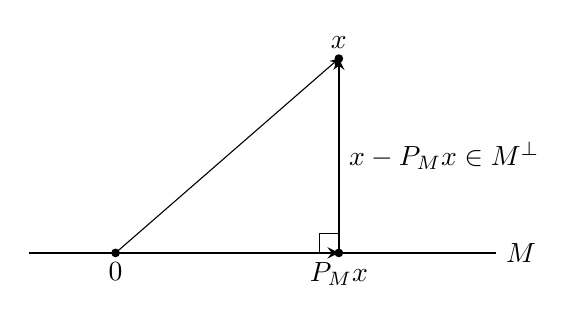
\begin{tikzpicture}[scale=1.05,>=stealth]
    \draw[thick] (-2.4,0)--(3.25,0) node[right] {$M$};
    \coordinate (O) at (-1.35,0);
    \coordinate (P) at (1.35,0);
    \coordinate (X) at (1.35,2.35);
    \fill (O) circle (1.5pt) node[below] {$0$};
    \fill (P) circle (1.5pt) node[below] {$P_Mx$};
    \fill (X) circle (1.5pt) node[above] {$x$};
    \draw[->,thick] (O)--(P);
    \draw[->,thick] (P)--(X) node[midway,right] {$x-P_Mx\in M^\perp$};
    \draw[->] (O)--(X);
    \draw (1.12,0)--(1.12,0.23)--(1.35,0.23);
  \end{tikzpicture}
  \caption[Hilbert 投影]{Hilbert 投影。向量 \(x\) 唯一分解为 \(M\) 内的最佳近似 \(P_Mx\) 与正交误差 \(x-P_Mx\)。}
  \label{b1:fig:hilbert-orthogonal-projection}
\end{figure}

在 \(L^2([0,1])\) 中取常数函数组成的子空间 \(M\)。由于 \(\|1\|_2=1\)，到该直线的投影为 \(P_Mf=\bigl(\int_0^1f(t)\,\mathrm dt\bigr)1\)。例如 \(f(t)=t\) 的最佳常数近似为 \(1/2\)，并有
\[
\int_0^1|t-a|^2\,\mathrm dt=\dfrac1{12}+\left|a-\dfrac12\right|^2.
\]
另一方面，去掉闭性后，\(\ell^2\) 中的 \(c_{00}\) 到向量 \((1/k)\) 的距离为零，却没有最小点；去掉凸性后，实直线中的闭集 \(\{-1,1\}\) 到 \(0\) 有两个最小点。

\ProseParagraphBreak

投影也给出一种具体的线性延拓。若 \(M\) 是 \(H\) 的闭子空间，\(Y\) 是赋范空间，且 \(A\in\mathcal B(M,Y)\)，则 \(\widetilde A=AP_M\) 定义在整个 \(H\) 上，在 \(M\) 上与 \(A\) 相同，并满足 \(\|\widetilde A\|\leq\|A\|\)。反过来，把 \(\widetilde A\) 限制到 \(M\) 的单位球上即得 \(\|A\|\leq\|\widetilde A\|\)，故两者范数相等。这里值域可以不止是一维；能作这种延拓的原因是定义域具有正交投影，而不是每个赋范空间都允许把向量值算子保范延拓。

\subsection{Riesz 表示定理}
\label{b1:subsec:080403}

固定 \(h\in H\)，映射 \(x\mapsto\langle x,h\rangle\) 是连续线性泛函。\term[riesz-biaoshi-hilbert]{Riesz 表示定理}[Riesz representation theorem]断言 Hilbert 空间中的每个连续线性泛函都以这种方式产生。对非零泛函，表示向量的方向由其核的正交补确定，尺度则由泛函的取值确定。

\begin{theorem}[Hilbert 空间的 Riesz 表示]\label{b1:thm:hilbert-riesz}
对实或复 Hilbert 空间 \(H\) 上的每个 \(\ell\in H^*\)，存在唯一 \(h\in H\) 满足 \(\ell(x)=\langle x,h\rangle\)（\(x\in H\)），且 \(\|\ell\|=\|h\|\)。
\end{theorem}
\begin{proof}
当 \(\ell=0\) 时取 \(h=0\)。否则取 \(u\) 使 \(\ell(u)=1\)。连续性保证 \(M=\ker\ell\) 闭。令 \(v=u-P_Mu\)，则 \(v\in M^\perp\)，且 \(\ell(v)=1\)，特别地 \(v\ne0\)。对任意 \(x\)，向量 \(x-\ell(x)v\) 属于 \(M\)，于是
\[
\langle x,v\rangle=\ell(x)\|v\|^2.
\]
取 \(h=v/\|v\|^2\) 就得到所需表示。若 \(h_1,h_2\) 都给出该表示，则 \(\langle x,h_1-h_2\rangle=0\) 对所有 \(x\) 成立；取 \(x=h_1-h_2\) 可知两者相等。

Cauchy--Schwarz 不等式给出 \(\|\ell\|\leq\|h\|\)。当 \(h\ne0\) 时，取单位向量 \(x=h/\|h\|\)，便有 \(|\ell(x)|=\|h\|\)，故范数相等；零向量情形亦成立。
\end{proof}

实空间中，映射 \(h\mapsto\langle\cdot,h\rangle\) 是线性等距满射；复空间中它却是共轭线性的，因为第二变量的系数要取共轭。因而“\(H\) 与 \(H^*\) 自然识别”在复情形下必须带上这一约定。特别地，对任意测度 \(\mu\)，每个 \(L^2(\mu)\) 上的连续线性泛函都唯一写成 \(f\mapsto\int_Xf\overline h\,\mathrm d\mu\)，其中 \(h\in L^2(\mu)\)；不需要额外的 \(\sigma\)-有限性假设。

\ProseParagraphBreak

若空间不完备，表示向量可能落在空间之外。在 \(c_{00}\) 上取从 \(\ell^2\) 限制而来的内积，令 \(\ell(x)=\sum_{n\geq1}x_n/n\)。每个输入只涉及有限和，有限维 Cauchy--Schwarz 不等式给出
\[
|\ell(x)|\leq\left(\sum_{n=1}^{\infty}\dfrac1{n^2}\right)^{1/2}\|x\|_2,
\]
故它连续。假如存在 \(h\in c_{00}\) 表示该泛函，依次代入各个单位坐标向量就会强制 \(\overline{h_n}=1/n\) 对所有 \(n\) 成立，与有限支撑矛盾。在完备空间 \(\ell^2\) 中，这个障碍消失，表示向量正是 \((1/n)\)。

\ProseParagraphBreak

表示定理还可以逐个处理算子的输出测试向量，得到谱理论所需的\term[bansui-suanzi]{伴随算子}[adjoint operator]。%
\footnote{孙炯等《泛函分析》第二版\cite{Sun2018Fanhan}第 5.3 节称为
“共轭算子”\termidx[gonge-suanzi]{共轭算子}。本节专指由 Hilbert 内积定义的伴随，
其值域是原 Hilbert 空间；后面在 Banach 对偶空间上定义的算子须另辨清定义域和值域。}

\begin{proposition}\label{b1:prop:hilbert-adjoint}
取 \(\mathbb K=\mathbb R\) 或 \(\mathbb C\)，各向量空间及线性映射均在同一标量域 \(\mathbb K\) 上。设 \(H,K\) 是同一标量域上的 Hilbert 空间，\(T\in\mathcal B(H,K)\)。存在唯一 \(T^*\in\mathcal B(K,H)\) 使
\[
\langle Tx,y\rangle_K=\langle x,T^*y\rangle_H
\quad(x\in H,\ y\in K).
\]
它满足 \(\|T^*\|=\|T\|\) 与 \((T^*)^*=T\)。这里 \(T^*\) 表示 Hilbert 空间上的伴随。
\end{proposition}
\symidx{\(T^*\)：Hilbert 空间上有界线性算子的伴随}
\begin{proof}
固定 \(y\in K\)，则 \(x\mapsto\langle Tx,y\rangle_K\) 是范数不超过 \(\|T\|\cdot\|y\|\) 的线性泛函。由\cref{b1:thm:hilbert-riesz}，它由唯一向量 \(T^*y\) 表示，且 \(\|T^*y\|\leq\|T\|\cdot\|y\|\)。对 \(a,b\in\mathbb K\)，有
\[
\langle x,T^*(ay+bz)\rangle
=\overline a\langle Tx,y\rangle+\overline b\langle Tx,z\rangle
=\langle x,aT^*y+bT^*z\rangle.
\]
表示的唯一性给出 \(T^*\) 的线性，前面的估计给出其有界性及 \(\|T^*\|\leq\|T\|\)。反向估计来自
\[
\|Tx\|=\sup_{\|y\|\leq1}|\langle Tx,y\rangle|
\leq\|T^*\|\cdot\|x\|;
\]
上确界等式由 Cauchy--Schwarz 不等式及 \(Tx\ne0\) 时取 \(y=Tx/\|Tx\|\) 得到。最后对伴随等式取共轭，便有 \(\langle T^*y,x\rangle=\langle y,Tx\rangle\)，唯一性给出 \((T^*)^*=T\)。
\end{proof}

例如有界可测函数 \(b\) 在 \(L^2(\mu)\) 上定义乘法算子 \(M_bf=bf\)。积分直接给出 \(\langle M_bf,g\rangle=\langle f,M_{\overline b}g\rangle\)，故 \(M_b^*=M_{\overline b}\)。复共轭在这里决定伴随算子的具体形式，不能因为实值例子中它消失就省略。

\subsection{正交系与正交基}
\label{b1:subsec:080404}

有限维空间中，正交坐标同时计算向量和长度。无限维情形还要决定无穷求和的意义，并检查坐标是否遗漏了整个子空间。Axler 的《Measure, Integration \& Real Analysis》\cite[Section 8C]{Axler2020Measure}并行讨论正交展开与最佳逼近；以下不预设空间可分。

\begin{definition}\label{b1:def:orthonormal-system}
取 \(\mathbb K=\mathbb R\) 或 \(\mathbb C\)，各向量空间及线性映射均在同一标量域 \(\mathbb K\) 上。设 \(H\) 是 Hilbert 空间。一族两两正交的非零向量称为\term[zhengjiao-xi]{正交系}[orthogonal system]；若每个向量的范数均为 \(1\)，则称为\term[biaozhun-zhengjiao-xi]{标准正交系}[orthonormal system]。若标准正交系 \((e_\alpha)_{\alpha\in I}\) 满足
\[
\overline{\operatorname{span}\{e_\alpha:\alpha\in I\}}=H,
\]
则称为 \(H\) 的\term[biaozhun-zhengjiao-ji]{标准正交基}[orthonormal basis]。这里的张成空间只含有限线性组合，再对它取范数闭包。%
\footnote{程其襄等《实变函数与泛函分析基础》第四版\cite{Cheng2019ShibianFanhan}%
第 9 章第 3 节使用“规范正交系”\termidx[guifan-zhengjiao-xi]{规范正交系}；
孙炯等《泛函分析》第二版\cite{Sun2018Fanhan}第 3.4.3 小节使用“标准正交基”。
本书采用“标准正交系／基”，单位长度条件不能省略。}
\end{definition}

对任意非负数族，约定 \(\sum_{\alpha\in I}a_\alpha\) 是其有限部分和的上确界。这使下面的\term[bessel]{Bessel 不等式}[Bessel's inequality]也适用于不可数指标集。

\begin{proposition}[Bessel]\label{b1:prop:bessel-inequality}
取 \(\mathbb K=\mathbb R\) 或 \(\mathbb C\)，各向量空间及线性映射均在同一标量域 \(\mathbb K\) 上。设 \(H\) 是 Hilbert 空间。若 \((e_\alpha)_{\alpha\in I}\) 是标准正交系，则每个 \(x\in H\) 满足
\[
\sum_{\alpha\in I}|\langle x,e_\alpha\rangle|^2\leq\|x\|^2.
\]
其中非零系数至多有可数个。
\end{proposition}
\begin{proof}
对有限集 \(F\subseteq I\)，令 \(s_F=\sum_{\alpha\in F}\langle x,e_\alpha\rangle e_\alpha\)。标准正交关系给出 \(x-s_F\) 与每个 \(e_\alpha\)（\(\alpha\in F\)）正交，因此
\[
\|x\|^2=\|x-s_F\|^2+\|s_F\|^2,
\quad
\|s_F\|^2=\sum_{\alpha\in F}|\langle x,e_\alpha\rangle|^2.
\]
取有限部分和的上确界即得不等式。对每个正整数 \(n\)，系数模长至少为 \(1/n\) 的指标只有有限个，否则可选足够大的有限集使平方和超过 \(\|x\|^2\)。非零指标集包含在这些有限集的可数并中。
\end{proof}

向量族的和 \(\sum_{\alpha\in I}x_\alpha=s\) 则按如下意义理解：对每个 \(\varepsilon>0\)，存在有限集 \(F_0\subseteq I\)，使任意包含 \(F_0\) 的有限集 \(F\) 都满足 \(\|s-\sum_{\alpha\in F}x_\alpha\|<\varepsilon\)。这是对有限部分和的要求，不需要给不可数集规定一个枚举次序。

\begin{theorem}[正交展开与 Parseval 恒等式]\label{b1:thm:orthonormal-expansion}
取 \(\mathbb K=\mathbb R\) 或 \(\mathbb C\)，各向量空间及线性映射均在同一标量域 \(\mathbb K\) 上。设 \(H\) 是 Hilbert 空间。设 \((e_\alpha)_{\alpha\in I}\) 是标准正交系，\(M\) 为其闭线性张成空间。则每个 \(x\in H\) 满足
\[
P_Mx=\sum_{\alpha\in I}\langle x,e_\alpha\rangle e_\alpha,
\quad
\|x-P_Mx\|^2=\|x\|^2-\sum_{\alpha\in I}|\langle x,e_\alpha\rangle|^2.
\]
以下条件等价：
\begin{equivalences}
  \item\label{b1:item:orthonormal-total} 该标准正交系是 \(H\) 的标准正交基；
  \item\label{b1:item:orthonormal-zero-complement} 与所有 \(e_\alpha\) 正交的向量只有零向量；
  \item\label{b1:item:orthonormal-parseval} 每个 \(x\in H\) 都满足\term[parseval-hengdengshi]{Parseval 恒等式}[Parseval's identity]，即 \(\|x\|^2=\sum_{\alpha\in I}|\langle x,e_\alpha\rangle|^2\)。
\end{equivalences}
这些条件成立时，\(x=\sum_{\alpha\in I}\langle x,e_\alpha\rangle e_\alpha\)，收敛均为范数收敛。
\end{theorem}
\begin{proof}
记 \(c_\alpha=\langle x,e_\alpha\rangle\)。Bessel 不等式使非零系数至多可数且平方可求和。若有无限多个，将它们列为 \((c_{\alpha_j})\)；相应部分和 \(s_n\) 满足
\[
\|s_m-s_n\|^2=\sum_{j=n+1}^{m}|c_{\alpha_j}|^2\longrightarrow0
\quad(m>n\to\infty).
\]
完备性给出 \(s_n\to s\in M\)，并且 \(\|s\|^2=\sum_{\alpha\in I}|c_\alpha|^2\)。对于任意含前 \(n\) 个非零指标的有限集 \(F\)，取足够大的 \(m\) 包含 \(F\) 中所有非零指标，再令 \(m\to\infty\)，得到
\[
\left\|s-\sum_{\alpha\in F}c_\alpha e_\alpha\right\|^2
=\sum_{\alpha\notin F}|c_\alpha|^2
\leq\sum_{j>n}|c_{\alpha_j}|^2.
\]
这证明了所规定的无序收敛，也说明极限不依赖枚举。有限或没有非零系数时直接取有限和或零即可。

内积连续性给出 \(\langle s,e_\alpha\rangle=c_\alpha\)，所以 \(x-s\) 与所有有限线性组合及其范数极限正交，即 \(x-s\in M^\perp\)。由\cref{b1:thm:hilbert-projection}，\(s=P_Mx\)，正交分解的平方范数等式给出余项公式。

第一项等价于 \(M=H\)。第二项等价于 \(M^\perp=\{0\}\)，由投影分解又等价于 \(M=H\)。余项公式表明第三项等价于每个 \(x\) 都属于 \(M\)。因此三项等价，展开式也随之成立。
\end{proof}

对标准正交基，两向量的内积也可以由坐标计算。Bessel 不等式说明两组坐标各自至多有可数个非零项；有限维 Cauchy--Schwarz 不等式又使坐标乘积族绝对可和。因此，下面右端按任意枚举所得的绝对收敛级数定义，其值与枚举无关：
\[
\langle x,y\rangle
=\sum_{\alpha\in I}\langle x,e_\alpha\rangle\overline{\langle y,e_\alpha\rangle}.
\]
有限部分和的内积具有这个形式，随后由内积连续性取极限即可；对任意有限指标集，坐标绝对值乘积的和均不超过 \(\|x\|\cdot\|y\|\)。若只有标准正交系，坐标则可能遗漏分量：\(\ell^2\) 中所有偶数坐标方向构成标准正交系，但第一单位向量的全部相应系数都为零。

\ProseParagraphBreak

正交展开还给出具体的最小二乘计算。在实空间 \(L^2([0,1])\) 中，\(e_0(t)=1\) 与 \(e_1(t)=\sqrt{12}(t-1/2)\) 构成一次多项式空间的标准正交基。对 \(f(t)=t^2\)，直接积分得
\[
\langle f,e_0\rangle=\dfrac13,
\quad
\langle f,e_1\rangle=\dfrac1{\sqrt{12}},
\quad
P_Mf(t)=t-\dfrac16.
\]
余项公式给出最小平方误差 \(1/5-1/9-1/12=1/180\)。因此投影并不只是存在性结论：一旦找出允许子空间的标准正交基，最佳近似及其误差就由有限个内积决定。

\begin{theorem}[标准正交基的存在]\label{b1:thm:orthonormal-basis-existence}
取 \(\mathbb K=\mathbb R\) 或 \(\mathbb C\)，各向量空间及线性映射均在同一标量域 \(\mathbb K\) 上。每个 Hilbert 空间都有标准正交基；其中任意给定的标准正交系都能扩充为标准正交基。
\end{theorem}
\begin{proof}
把包含给定标准正交系的所有标准正交子集按包含关系排序。任一链的并仍是标准正交集：并集中任意两个向量都属于链中某个共同成员，故保留正交关系与单位长度。空链也有给定集合这个上界。由 Zorn 引理存在极大者 \(E\)。若 \(E^\perp\) 含非零向量 \(u\)，则加入 \(u/\|u\|\) 就得到更大的标准正交集，矛盾。因此 \(E^\perp=\{0\}\)，由\cref{b1:thm:orthonormal-expansion}知 \(E\) 是标准正交基。初始集合取空集便得存在性；\(H=\{0\}\) 时空集本身就是所需基。
\end{proof}

在可分空间中，取可数稠密集 \(\{x_n:n\geq1\}\)。处理 \(x_n\) 时，设已保留的标准正交向量为 \(e_1,\ldots,e_r\)，令
\[
v_n=x_n-\sum_{j=1}^r\langle x_n,e_j\rangle e_j.
\]
若 \(v_n=0\) 就略过；否则加入 \(v_n/\|v_n\|\)。内积计算表明新方向与旧方向正交，而已处理的每个 \(x_n\) 都属于已保留向量的线性张成。因而最后得到的有限或可数标准正交系的闭线性张成包含稠密集，必为整个空间。这就是\term[gram-schmidt-zhengjiaohua]{Gram--Schmidt 正交化}[Gram--Schmidt orthogonalization]，它不替代上面对不可分空间的论证。

\ProseParagraphBreak

例如在任意集合 \(I\) 的幂集上取计数测度，所得 \(L^2\) 记为 \(\ell^2(I)\)，各单点示性函数构成标准正交基：与它们全部正交的函数每个坐标都为零。若 \(I\) 不可数，这些单位向量两两距离为 \(\sqrt2\)，以它们为中心、半径 \(1/3\) 的开球两两不交，可数稠密集不可能同时与所有这些球相交，故空间不可分。

\ProseParagraphBreak

标准正交基的“基”允许范数极限，不是只允许有限展开的代数基。对 \(L^2\) 而言，展开等式也只是等价类之间的平方积分收敛，并不自动给出逐点收敛。这两个区别决定了下一节中谱展开的准确含义。

% !TeX root = ../../Book1.tex
\OptionalSection{紧算子与紧自伴谱理论}{b1:sec:0805}

有限维自伴矩阵可以选取一组标准正交特征向量，使矩阵化为实对角形。
无穷维空间中的有界自伴算子未必有特征向量，更不能直接套用这一结论。
本节增加紧性假设，证明非零特征空间与零特征空间共同给出完整的正交分解；
末尾再把这一分解用于区间上的一个边值问题。


\ProseParagraphBreak

本节及章末带星号的四道习题可留作选读；具体的边值问题展示了特征展开如何帮助求解方程。

\ProseParagraphBreak

关于紧算子的基本运算和紧自伴谱定理，见 Axler 的《Measure, Integration \& Real Analysis》\cite[Sections 10C and 10D]{Axler2020Measure}。

\subsection{紧算子}
\label{b1:subsec:080501}

考虑单位球中的一列向量。如果算子作用以后总能从像中取出一个收敛子列，
那么许多有限维极限论证便有机会继续使用。紧算子把这一要求应用于所有有界列。

\begin{definition}[紧算子]
\label{b1:def:compact-operator}
取 \(\mathbb K=\mathbb R\) 或 \(\mathbb C\)，各向量空间及线性映射均在同一标量域 \(\mathbb K\) 上。设 \(X,Y\) 为赋范空间，\(T:X\to Y\) 为线性算子。若对 \(X\) 中每个有界列 \((x_n)\)，
像列 \((Tx_n)\) 都有在 \(Y\) 中收敛的子列，则称 \(T\) 为%
\term[jin-suanzi]{紧算子}[compact operator]%
\nobreak\mbox{。\footnotemark}
\footnotetext{程其襄等《实变函数与泛函分析基础》第四版\cite{Cheng2019ShibianFanhan}%
第 11 章使用“全连续算子”\termidx[quanlianxu-suanzi]{全连续算子}。
本节固定使用“紧算子”及上述有界列定义；遇到以弱收敛列或非线性映射表述的
“全连续”时，仍须核对其定义，不能仅凭名称直接互换。}
\end{definition}

这个定义已经蕴含有界性：若 \(T\) 在单位球上无界，可以选取%
\(\|x_n\|\leq1\) 而 \(\|Tx_n\|\geq n\)，与定义矛盾。
值域有限维的线性算子称为\term[youxianzhi-suanzi]{有限秩算子}[finite-rank operator]。
有界的有限秩算子是紧算子，因为其像落在有限维子空间内，
而有限维空间的有界列有收敛子列。有限秩本身不能代替有界性：
一个不连续线性泛函的值域也只有一维。

\begin{proposition}[紧算子的运算]
\label{b1:prop:compact-operator-calculus}
取 \(\mathbb K=\mathbb R\) 或 \(\mathbb C\)，各向量空间及线性映射均在同一标量域 \(\mathbb K\) 上。设 \(X,Y,Z\) 是赋范空间。以下线性组合的算子均从 \(X\) 到 \(Y\)，复合的算子具有匹配的定义域和值域。紧算子的线性组合仍为紧算子。紧算子与有界线性算子在任一侧作有意义的复合，
所得算子仍为紧算子。若 \(Y\) 是 Banach 空间，且紧算子列%
\(T_n:X\to Y\) 在算子范数下收敛于 \(T\)，则 \(T\) 紧。
\end{proposition}

\begin{proof}
对有界列先取子列使第一个紧算子的像收敛，再从中取子列使第二个像收敛，
便得到线性组合的结论。右侧的有界算子把有界列送到有界列；
左侧的有界算子保持已经得到的极限，故两种复合都紧。

设 \(\|T_n-T\|\to0\)，且 \(\|x_j\|\leq M\)。
逐次取子列，使 \(T_1x_j,T_2x_j,\ldots\) 依次收敛，再取对角子列 \((x_{j_k})\)。
对每个固定的 \(n\)，\((T_nx_{j_k})_k\) 都是 Cauchy 列，而
\[
 \|Tx_{j_k}-Tx_{j_l}\|
 \leq 2M\|T-T_n\|+\|T_nx_{j_k}-T_nx_{j_l}\|.
\]
先取 \(n\) 使第一项小，再取 \(k,l\) 使第二项小。
由 \(Y\) 完备，\((Tx_{j_k})\) 收敛，故 \(T\) 紧。
\end{proof}

值域的完备性在最后一步发挥作用；只得到 Cauchy 子列还不能代替定义中的收敛子列。
这个命题也给出一种常用的紧性证明方法：用有限秩算子在算子范数下逼近。
本节使用的积分算子都可这样处理，但这里并未断言任意 Banach 空间上的紧算子
都能作这种逼近。

\ProseParagraphBreak

设 \((a_n)\) 为有界标量列，在 \(\ell^2\) 上定义 \(D_ax=(a_nx_n)_n\)。
有 \(\|D_a\|=\sup_n|a_n|\)，并且 \(D_a\) 紧当且仅当 \(a_n\to0\)。
事实上，截断到前 \(N\) 个坐标得到有限秩算子 \(D_a^{(N)}\)，且
\[
 \|D_a-D_a^{(N)}\|=\sup_{n>N}|a_n|.
\]
若 \(a_n\not\to0\)，则存在 \(\varepsilon>0\) 及无穷多个指标满足%
\(|a_n|\geq\varepsilon\)。相应的单位向量 \(e_n\) 的像两两距离至少为%
\(\sqrt2\,\varepsilon\)，没有收敛子列。
特别地，无穷维 Hilbert 空间上的恒等算子不紧：任取一列标准正交向量即可作同样的反证。

\subsection{紧自伴算子}
\label{b1:subsec:080502}

\begin{definition}[自伴算子]
\label{b1:def:self-adjoint-operator}
取 \(\mathbb K=\mathbb R\) 或 \(\mathbb C\)，各向量空间及线性映射均在同一标量域 \(\mathbb K\) 上。设 \(T\) 是 Hilbert 空间 \(H\) 上的有界线性算子。若 \(T=T^*\)，则称 \(T\) 为%
\term[zi-ban-suanzi]{自伴算子}[self-adjoint operator]。%
\footnote{孙炯等《泛函分析》第二版\cite{Sun2018Fanhan}第 5.4 节使用
“自共轭”\termidx[zi-gonge-suanzi]{自共轭算子}这一名称。
这里讨论定义在整个 Hilbert 空间上的有界算子；对一般无界算子，
不能只检查形式上的内积等式而省略定义域条件。}%
按照本章内积对第一变量线性的约定，这等价于
\[
 \langle Tx,y\rangle=\langle x,Ty\rangle\quad(x,y\in H).
\]
\end{definition}

于是 \(\langle Tx,x\rangle\) 总为实数。
若 \(Tx=\lambda x\) 且 \(x\ne0\)，则
\(\lambda\|x\|^2=\langle Tx,x\rangle\)，所以特征值 \(\lambda\) 为实数。
若 \(Ty=\mu y\) 且 \(\lambda\ne\mu\)，自伴性又给出%
\((\lambda-\mu)\langle x,y\rangle=0\)，故不同特征值的特征空间相互正交。

\ProseParagraphBreak

自伴性还不足以保证特征向量存在。例如在 \(L^2(0,1)\) 上令 \(Sf(x)=x\cdot f(x)\)，
由前节的乘法算子计算可知 \(S\) 有界且自伴。
若 \(Sf=\lambda f\)，则 \(f\) 只能在集合 \(\{x:x=\lambda\}\) 上非零；
这个集合的测度为零，故 \(f\) 是零等价类。因此 \(S\) 没有特征值。

\ProseParagraphBreak

还有一个与有限维情形同样重要的事实。若子空间 \(M\) 在 \(T\) 下不变，
则 \(M^\perp\) 也在 \(T\) 下不变：对 \(y\in M^\perp\)、\(x\in M\)，有%
\(\langle Ty,x\rangle=\langle y,Tx\rangle=0\)。
当 \(M\) 闭时，\(T\) 在 \(M^\perp\) 上的限制仍是自伴算子；若原算子紧，这个限制也紧。
因而在找到一些特征向量以后，可以继续研究它们张成的闭子空间的正交补。
首先必须证明：只要限制算子非零，就确实还有特征向量可找。

\begin{lemma}[模最大的特征值]
\label{b1:lem:compact-self-adjoint-extreme}
取 \(\mathbb K=\mathbb R\) 或 \(\mathbb C\)，各向量空间及线性映射均在同一标量域 \(\mathbb K\) 上。设 \(H\) 是 Hilbert 空间。非零紧自伴算子 \(T:H\to H\) 至少有一个特征值 \(\lambda\) 满足%
\(|\lambda|=\|T\|\)。
\end{lemma}

\begin{proof}
记 \(q(x)=\langle Tx,x\rangle\)，以及%
\(m=\sup_{\|x\|=1}|q(x)|\)。先证明 \(m=\|T\|\)。
显然 \(m\leq\|T\|\)。对单位向量 \(x,y\)，利用自伴性和实部的极化关系，
\[
 4\operatorname{Re}\langle Tx,y\rangle=q(x+y)-q(x-y),
\]
从而
\[
 |\operatorname{Re}\langle Tx,y\rangle|
 \leq \frac m4\bigl(\|x+y\|^2+\|x-y\|^2\bigr)=m.
\]
若 \(Tx\ne0\)，取 \(y=Tx/\|Tx\|\)，左边就是 \(\|Tx\|\)，故 \(\|T\|\leq m\)。

取单位向量列，使 \(|q(x_n)|\to\|T\|\)。取子列后，可以设%
\(q(x_n)\to\lambda\)，其中 \(\lambda=\|T\|\) 或 \(-\|T\|\)。
由于 \(\lambda\) 为实数，
\[
 \|Tx_n-\lambda x_n\|^2
 =\|Tx_n\|^2-2\lambda\cdot q(x_n)+\lambda^2
 \leq2\|T\|^2-2\lambda\cdot q(x_n)\longrightarrow0.
\]
紧性给出子列 \(Tx_{n_k}\to v\)。因 \(\lambda\ne0\)，上式又给出%
\(x_{n_k}\to x=v/\lambda\)。于是 \(\|x\|=1\)，且由连续性 \(Tx=\lambda x\)。
\end{proof}

证明中最大值不是事先假设存在的。先用上确界得到近似特征向量，
再用紧性把近似向量变成真正的特征向量，这正是无限维论证需要补上的一步。

\subsection{谱定理}
\label{b1:subsec:080503}

\begin{theorem}[紧自伴谱定理]
\label{b1:thm:compact-self-adjoint-spectral}
取 \(\mathbb K=\mathbb R\) 或 \(\mathbb C\)，各向量空间及线性映射均在同一标量域 \(\mathbb K\) 上。设 \(H\) 是 Hilbert 空间。设 \(T:H\to H\) 是紧自伴算子。存在有限个或可数个标准正交向量 \(e_n\)，
以及相应的非零实特征值 \(\lambda_n\)，使
\[
 H=\ker T\oplus\overline{\operatorname{span}}\{e_n\},\quad
 Tx=\sum_n\lambda_n\langle x,e_n\rangle e_n.
\]
每个非零特征值只有有限重数；若向量列为无穷列，则 \(\lambda_n\to0\)。
级数在 \(H\) 的范数下收敛，而且有限秩算子
\[
 T_Nx=\sum_{n=1}^N\lambda_n\langle x,e_n\rangle e_n
\]
满足 \(\|T-T_N\|=\sup_{n>N}|\lambda_n|\to0\)。
有限列情形中，各个和只遍历实际存在的指标，空尾部的上确界按零处理；
\(T=0\) 时取空列。
\end{theorem}

\begin{proof}
固定 \(\varepsilon>0\)。属于绝对值至少为 \(\varepsilon\) 的特征值的标准正交向量
不可能有无穷多个，因为它们的像两两距离至少为 \(\sqrt2\,\varepsilon\)，违反紧性。
特别地，每个非零特征空间都有限维；对每个正整数 \(k\)，绝对值至少为 \(1/k\)
的非零特征值只有有限个。因此所有非零特征值组成至多可数集。
在各非零特征空间中选取有限标准正交基，合起来记为 \(\{e_n\}\)。
不同特征空间的正交性保证这仍是标准正交系。若它无穷，则对任意%
\(\varepsilon>0\)，至多有限个 \(\lambda_n\) 满足 \(|\lambda_n|\geq\varepsilon\)，
所以 \(\lambda_n\to0\)。

令 \(M=\overline{\operatorname{span}}\{e_n\}\)。
由 \(T\) 连续，\(M\) 在 \(T\) 下不变；因此 \(M^\perp\) 也不变。
若 \(T|_{M^\perp}\ne0\)，则由\cref{b1:lem:compact-self-adjoint-extreme}，
在 \(M^\perp\) 中存在一个非零特征值的特征向量。
但它属于前面已经全部收入 \(M\) 的某个特征空间，矛盾。
于是 \(M^\perp\subseteq\ker T\)。反过来，若 \(Tx=0\)，则
\[
 0=\langle Tx,e_n\rangle=\langle x,Te_n\rangle
   =\lambda_n\langle x,e_n\rangle
\]
对每个 \(n\) 成立，故 \(x\in M^\perp\)。这证明 \(M^\perp=\ker T\)。

将 \(x\) 按此正交直和分解，并应用\cref{b1:thm:orthonormal-expansion}，
再用 \(T\) 的连续性，就得到所述展开。
最后由正交性，
\[
 \|(T-T_N)x\|^2
 =\sum_{n>N}|\lambda_n|^2\cdot|\langle x,e_n\rangle|^2
 \leq\bigl(\sup_{n>N}|\lambda_n|\bigr)^2\|x\|^2.
\]
逐个取 \(x=e_n\)，\(n>N\)，又得到反向的范数下界，故余项范数等式成立。
\end{proof}

定理没有假定 \(H\) 可分。非零特征值对应的部分确实可分，
但 \(\ker T\) 可以不可分；不能由紧性推出整个空间存在可数标准正交基。
如果愿意把核空间也写成坐标形式，可以在其中另选标准正交基，并赋予特征值零。

\ProseParagraphBreak

在复 Hilbert 空间中，通常把使 \(T-zI\) 不可逆的复数 \(z\) 组成的集合称为算子的%
\term[pu]{谱}[spectrum]，记为 \(\sigma(T)\)。
\symidx{\(\sigma(T)\)：有界算子的谱}
这里可逆指存在定义在全空间上的有界逆。
上一定理立即说明：对于紧自伴 \(T\)，每个非零谱点都是特征值。
事实上，若 \(z\ne0\) 且不等于任何 \(\lambda_n\)，则 \(\lambda_n\to0\)
保证它到这些数的距离为正。在分解 \(x=x_0+\sum_n c_ne_n\) 上，
\[
 (T-zI)^{-1}x=-\frac{x_0}{z}+\sum_n\frac{c_n}{\lambda_n-z}e_n
\]
定义了有界的双侧逆。在无穷维空间中，零必在谱内：
否则 \(I=T^{-1}T\) 将是紧算子。
但零未必是特征值，这一点不可与有限维矩阵混同。

\ProseParagraphBreak

在 \(\ell^2\) 上令 \(Te_n=n^{-1}e_n\)。这个算子紧、自伴而且单射，
所以零不是特征值，但由上述论证零在谱内。
向量 \(y=(1/n)_n\) 属于 \(\ell^2\)，却不属于 \(T\) 的值域：
唯一可能的原像是并不属于 \(\ell^2\) 的常数列 \((1)_n\)。
另一方面，\(y\) 的有限截断都在值域内，并趋于 \(y\)。
因此值域不闭。逆映射虽能在值域上定义，却不有界，因为%
\(\|e_n\|/\|Te_n\|=n\)。谱展开中的小特征值，正好刻画了反求原像时误差被放大的原因。

\subsection{Dirichlet Green 算子与正弦展开}
\label{b1:subsec:080504}

考虑最简单的 Dirichlet 边值问题
\[
 -u''=f\quad(0<x<1),\quad u(0)=u(1)=0.
\]
把右端函数映到相应的解，便得到这个方程的解算子。
定义
\[
 K(x,y)=\min(x,y)-xy,\quad
 (Gf)(x)=\int_0^1K(x,y)\cdot f(y)\,\mathrm{d}y.
\]
这个核称为本问题的\term[green-hanshu]{Green 函数}[Green function]。
下文在 \(L^2(0,1)\) 上研究 \(G\)；这个空间的完备性已由%
\cref{b1:thm:l2-hilbert}建立。

\begin{proposition}[Dirichlet 问题的 Green 算子]
\label{b1:prop:dirichlet-green}
取 \(\mathbb K=\mathbb R\) 或 \(\mathbb C\)，各向量空间及线性映射均在同一标量域 \(\mathbb K\) 上。在 \((0,1)\) 的 Lebesgue 测度下定义
\[
 (Gf)(x)=\int_0^1(\min(x,y)-xy)\cdot f(y)\,\mathrm dy.
\]
算子 \(G:L^2(0,1;\mathbb K)\to L^2(0,1;\mathbb K)\) 紧、自伴、单射，且%
\(\langle Gf,f\rangle\geq0\)。
若 \(f\) 连续，则 \(u=Gf\) 是边值问题 \(-u''=f\)（\(0<x<1\)）、\(u(0)=u(1)=0\) 的唯一的经典解。
\end{proposition}

\begin{proof}
对任意平方可积核 \(L\)，Cauchy--Schwarz 不等式给出
\[
 \left\|\int_0^1L(\,\cdot\,,y)\cdot f(y)\,\mathrm{d}y\right\|_2
 \leq \|L\|_{L^2\bigl((0,1)^2\bigr)}\cdot\|f\|_2.
\]
这既证明 \(G\) 有界，也估计了用另一个核替代 \(K\) 所产生的算子范数误差。
将单位正方形细分为网格，在每个小矩形内用一个取值代替 \(K\)。
由 \(K\) 一致连续，所得阶梯核 \(K_N\) 一致收敛于 \(K\)。
每个 \(K_N\) 是有限个形如 \(c\cdot\mathbf1_A(x)\cdot\mathbf1_B(y)\) 的函数之和，
故其积分算子有限秩。上述估计和\cref{b1:prop:compact-operator-calculus}证明 \(G\) 紧。
由 \(K(x,y)=K(y,x)\) 为实数，Fubini 定理给出%
\(\langle Gf,g\rangle=\langle f,Gg\rangle\)。
换序合法，因为 \(f,g\in L^1(0,1)\)，且 \(K\) 有界。

为同时证明非负性和单射性，注意恒等式
\[
 K(x,y)=\int_0^1(\mathbf1_{\{t<x\}}-x)(\mathbf1_{\{t<y\}}-y)\,\mathrm{d}t.
\]
再次应用 Fubini 定理，可得
\[
 \langle Gf,f\rangle=\int_0^1|Af(t)|^2\,\mathrm{d}t,\quad
 Af(t)=\int_t^1 f(y)\,\mathrm{d}y-\int_0^1y\cdot f(y)\,\mathrm{d}y.
\]
因此二次型非负。若 \(Gf=0\)，则 \(Af=0\) 几乎处处。
而 \(|Af(t)-Af(s)|\leq\|f\|_2\cdot|t-s|^{1/2}\)，故 \(Af\) 连续，因而处处为零。
这说明 \(f\) 在每个区间上的积分均为零。
为从这里得到 \(f=0\) 几乎处处，令 \(\nu(E)=\int_E f\,\mathrm{d}y\)。
这是有限复测度；由于 \(\nu\bigl((0,1)\bigr)=0\)，满足 \(\nu(E)=0\) 的 Borel 集构成
包含所有区间的 Dynkin 系。由 \(\pi\)--\(\lambda\) 定理，\(\nu\) 在所有 Borel 集上为零。
Lebesgue 可测集与 Borel 集至多相差零测集，所以同样有 \(\int_E f=0\)。
分别取实部和虚部的正、负水平集，就得到 \(f=0\) 几乎处处。

最后，若 \(f\) 连续，将积分在 \(y=x\) 处分开：
\[
 u(x)=(1-x)\cdot\int_0^x y\cdot f(y)\,\mathrm{d}y
       +x\int_x^1(1-y)\cdot f(y)\,\mathrm{d}y.
\]
由初等微积分直接求导得 \(u''=-f\)，端点值均为零。
任意两个经典解之差的二阶导数为零，因而是仿射函数；
再由两个端点值为零，差只能为零。
\end{proof}

现在可以把抽象谱定理转化为一个熟悉的具体结论，而且不会预先假设正弦系完备。

\begin{corollary}[区间上的正弦展开]
\label{b1:cor:dirichlet-sine-basis}
取 \(\mathbb K=\mathbb R\) 或 \(\mathbb C\)，各向量空间及线性映射均在同一标量域 \(\mathbb K\) 上。在区间 \((0,1)\) 的 Lebesgue 测度下，令 \((Gf)(x)=\int_0^1(\min(x,y)-xy)f(y)\,\mathrm dy\)。函数 \(e_n(x)=\sqrt2\cdot \sin(n\pi x)\)，\(n\geq1\)，组成 \(L^2(0,1)\) 的标准正交基，
且 \(Ge_n=(n\pi)^{-2}e_n\)。对每个 \(f\in L^2(0,1)\)，
\[
 Gf=\sum_{n=1}^{\infty}
       \frac{\langle f,e_n\rangle}{(n\pi)^2}e_n
\]
在 \(L^2\) 范数下成立。
\end{corollary}

\begin{proof}
若 \(Gf=\lambda f\)、\(f\ne0\)、\(\lambda\ne0\)，则由非负性知 \(\lambda>0\)。
连续核的积分 \(Gf\) 是连续函数：核关于 \(x\) 的一致连续性与%
\(f\in L^1\) 保证其连续性。因此可为 \(f=\lambda^{-1}Gf\) 选取连续代表元。
再用\cref{b1:prop:dirichlet-green}的经典解结论，得到
\[
 -f''=\lambda^{-1}f,\quad f(0)=f(1)=0.
\]
解这个常系数微分方程可知，非零解存在当且仅当%
\(\lambda=(n\pi)^{-2}\)，其解空间由 \(\sin(n\pi x)\) 张成。
反过来，利用经典边值问题的唯一性，每个 \(e_n\) 确是所列特征值的特征函数。
直接积分给出 \(\|e_n\|_2=1\)；不同特征值的特征函数相互正交。
由于 \(G\) 单射，紧自伴谱定理中的核空间为零，故这些函数张成的闭子空间就是全部%
\(L^2(0,1)\)。谱定理也同时给出 \(Gf\) 的展开。
\end{proof}

这个例子显示了 Sturm--Liouville 理论的一条基本路径：先解边值问题，
证明解算子紧且自伴，再用谱分解寻找特征函数。
本节只处理常系数、有限区间和齐次 Dirichlet 条件这一模型。
一般系数、奇异端点和无界算子的定义域都需要另外讨论，
不能把上述证明中的连续核和经典求导步骤不加检查地搬过去。
但即使在这个最简单的情形，紧性、投影、正交展开与积分换序已经共同参与了论证。

% 本章小结（不计入编号）
\begin{chaptersummary}
范数、完备性和线性结构承担不同的任务。算子范数把连续性转化成误差估计，
完备性保证误差可求和的逼近列在原空间中收敛；有限维范数等价和闭有界集紧致，
则不能无条件搬到函数空间中。

\ProseParagraphBreak

Hahn--Banach 定理先保证泛函可以保范延拓，再由凸集的 Minkowski 泛函导出分离。
它使对偶范数准确恢复每个向量的长度，却不保证延拓唯一。
Baire 纲定理提供另一种存在性机制：把可数覆盖中的局部信息转为一致控制。
一致有界、开映射和闭图像定理分别据此处理算子族、求解稳定性和连续性检验。

\ProseParagraphBreak

Hilbert 空间的内积增加了正交几何。最近点由平行四边形恒等式得到，
投影又导出 Riesz 表示和正交展开。一般正交基可以不可数，
但每个向量至多具有可数个非零坐标；函数展开的范数收敛也不等于逐点收敛。
在选读部分，紧自伴谱定理进一步把算子本身作有限秩逼近，Green 算子的例子则把这种逼近
落实为正弦特征函数。下一章将研究较弱的收敛方式，
以应对有界列在原范数下通常没有收敛子列这一困难。
\end{chaptersummary}


\BookExercises

% 下列题目按本章证明工具综合组织，非逐字摘录；
% 背景定位：Axler2020Measure 6C--E（完备性、延拓、对偶、算子原理）、
% 8B--C（投影与正交坐标）、10C--D（紧算子和谱分解）。
% 商空间距离公式、极限泛函和Volterra为经典训练主题，补完整题设与解答；
% Green共振题为本章边值模型的继续推导。均不要求未写章节的结果。

% 自拟：把向量嵌入二次对偶，直接训练算子范数与一致有界原理。
\begin{exercise}\label{b1:ex:08-uniform-bounded-vectors}
设 \(X\) 是赋范空间，\((x_n)\subset X\)，并且对每个 \(f\in X^*\)，数列 \((f(x_n))\) 都有界。对 \(n\geq1\)，定义
\[
J_n:X^*\longrightarrow\mathbb K,\qquad J_n(f)=f(x_n).
\]
证明 \(J_n\) 是有界线性泛函且 \(\|J_n\|=\|x_n\|\)，再用一致有界原理证明 \((x_n)\) 在 \(X\) 中范数有界。说明为什么这里不需要假设 \(X\) 完备。
\end{exercise}
\begin{solution}
线性由定义得到，而
\[
|J_n(f)|=|f(x_n)|\leq\|f\|\cdot\|x_n\|
\]
给出 \(\|J_n\|\leq\|x_n\|\)。若 \(x_n\ne0\)，\cref{b1:cor:norming-functional}给出 \(f_n\in X^*\)，使 \(\|f_n\|=1\)、\(|f_n(x_n)|=\|x_n\|\)，故反向不等式成立；\(x_n=0\) 时范数等式直接成立。

题设正是
\[
\sup_n|J_n(f)|<\infty\qquad(f\in X^*).
\]
对 Banach 空间 \(X^*\) 上的算子族 \(\{J_n:n\geq1\}\) 应用一致有界原理，得到
\[
\sup_n\|x_n\|=\sup_n\|J_n\|<\infty.
\]
定义域是 \(X^*\)，而连续对偶总是 Banach 空间；原空间 \(X\) 是否完备不参与这次应用。
\end{solution}

% 自拟：训练有界逆定理给出的下界及其对闭值域的直接作用。
\begin{exercise}\label{b1:ex:08-bounded-below-closed-range}
设 \(X\) 是 Banach 空间，\(Y\) 是赋范空间，\(T\in\mathcal B(X,Y)\)。若存在 \(c>0\)，使
\[
\|Tx\|\geq c\|x\|\qquad(x\in X),
\]
证明 \(T\) 单射、\(T(X)\) 闭，且 \(T^{-1}:T(X)\to X\) 有界。反过来，设 \(X,Y\) 都是非零 Banach 空间且 \(T:X\to Y\) 是有界线性双射；用有界逆定理证明上述下界对某个 \(c>0\) 成立。
\end{exercise}
\begin{solution}
下界立即说明 \(Tx=0\) 只能发生在 \(x=0\)，故 \(T\) 单射。若 \(Tx_n\to y\) 于 \(Y\)，则
\[
c\|x_n-x_m\|\leq\|Tx_n-Tx_m\|,
\]
所以 \((x_n)\) 是 Cauchy 列。由 \(X\) 完备，存在 \(x\in X\) 使 \(x_n\to x\)；再由 \(T\) 连续，\(Tx_n\to Tx\)，从而 \(y=Tx\in T(X)\)。因此值域闭。对 \(y=Tx\in T(X)\)，同一估计给出
\[
\|T^{-1}y\|=\|x\|\leq c^{-1}\|y\|,
\]
故逆算子有界。

反过来，有界逆定理给出 \(T^{-1}\in\mathcal B(Y,X)\)。因为空间非零，\(\|T^{-1}\|>0\)，并且
\[
\|x\|=\|T^{-1}Tx\|\leq\|T^{-1}\|\,\|Tx\|.
\]
取 \(c=\|T^{-1}\|^{-1}\) 即得所需下界。
\end{solution}

% 自拟：用对角乘子把“处处有定义加闭图像”转化为统一系数界。
\begin{exercise}\label{b1:ex:08-closed-graph-diagonal}
设 \((a_n)\) 是任意标量序列，并假设对每个 \(x=(x_n)\in\ell^1\)，序列 \((a_nx_n)\) 仍属于 \(\ell^1\)。定义
\[
D_a:\ell^1\longrightarrow\ell^1,\qquad D_ax=(a_nx_n).
\]
先证明 \(D_a\) 的图像闭，再用闭图像定理证明 \((a_n)\in\ell^\infty\)，并求 \(\|D_a\|\)。最后证明 \((a_n)\in\ell^\infty\) 也足以保证 \(D_a\) 在整个 \(\ell^1\) 上有定义。
\end{exercise}
\begin{solution}
设 \(x^{(k)}\to x\) 且 \(D_ax^{(k)}\to y\) 都在 \(\ell^1\) 中成立。每个坐标泛函在 \(\ell^1\) 上连续，因此对固定 \(n\)，有
\[
x_n^{(k)}\to x_n,\qquad a_nx_n^{(k)}\to y_n.
\]
标量极限唯一性给出 \(y_n=a_nx_n\)。题设保证 \(D_ax\in\ell^1\)，所以 \(y=D_ax\)，图像闭。定义域和值域都是 Banach 空间，闭图像定理因而给出 \(D_a\) 有界。

对第 \(n\) 个单位向量 \(e_n\)，有
\[
|a_n|=\|D_ae_n\|_1\leq\|D_a\|,
\]
故 \(a\in\ell^\infty\)。反过来，若 \(a\in\ell^\infty\)，则
\[
\|D_ax\|_1=\sum_n|a_nx_n|
\leq\|a\|_\infty\|x\|_1,
\]
所以 \(D_a\) 处处有定义且 \(\|D_a\|\leq\|a\|_\infty\)。再用单位向量并对 \(n\) 取上确界，得到 \(\|D_a\|=\|a\|_\infty\)。
\end{solution}

\begin{exercise}\label{b1:ex:08-quotient-dual}
设 \(X\) 是 Banach 空间，\(M\subset X\) 是闭线性子空间，\(Q:X\to X/M\) 是商映射。利用\cref{b1:thm:quotient-banach}与\cref{b1:prop:quotient-dual}证明：对每个 \(x\in X\) 和 \(r>0\)，都有
\[
Q\bigl(B_X(x,r)\bigr)=B_{X/M}(Qx,r),
\]
并且
\[
\operatorname{dist}(x,M)
=\sup\{\,|f(x)|:f\in M^\circ,\ \|f\|\leq1\,\}.
\]
最后指出：若把第一式中的开球改成闭球，同一证明会在哪一步失效。
\end{exercise}
\begin{solution}
若 \(z\in B_X(x,r)\)，则
\[
\|Qz-Qx\|=\|Q(z-x)\|\leq\|z-x\|<r,
\]
所以左边包含于右边。反过来，若 \(u\in B_{X/M}(Qx,r)\)，则 \(\|u-Qx\|<r\)。按商范数的下确界定义，可以为 \(u-Qx\) 选取代表 \(v\in X\)，使 \(Qv=u-Qx\) 且 \(\|v\|<r\)。于是 \(u=Q(x+v)\)，而 \(x+v\in B_X(x,r)\)。这证明开球等式。

商范数定义给出 \(\operatorname{dist}(x,M)=\|Qx\|\)。对 \(X/M\) 中的向量 \(Qx\) 使用\cref{b1:cor:norming-functional}，再由\cref{b1:prop:quotient-dual}把 \((X/M)^*\) 的单位球等距拉回 \(M^\circ\) 的单位球，便得到所述上确界公式。

开球的反向包含使用了严格不等式 \(\|u-Qx\|<r\)，因而能从下确界中选到范数严格小于 \(r\) 的代表。若只有 \(\|u-Qx\|\leq r\)，边界情形会要求这个下确界实际取得；一般闭子空间未必为每个向量提供最佳逼近，所以同一论证不能推出闭球等式。
\end{solution}

\begin{exercise}\label{b1:ex:08-c0-dual}
令 \(c_0\) 为趋于零的标量序列空间，取一致范数；
令 \(\ell^1=\{a:\sum_n|a_n|<\infty\}\)，取范数 \(\|a\|_1=\sum_n|a_n|\)。
证明 \(c_0\) 是 Banach 空间，每个 \(F\in c_0^*\) 都唯一表示为
\[
 F(x)=\sum_{n=1}^\infty a_nx_n,\quad a\in\ell^1,
\]
且 \(\|F\|=\|a\|_1\)。
\end{exercise}
\symidx{\(c_0\)：趋于零的标量序列空间}
\symidx{\(\ell^1\)：绝对可求和的标量序列空间}
\begin{solution}
若 \(x^{(j)}\to x\) 一致且各 \(x^{(j)}\in c_0\)，给定 \(\varepsilon>0\)，
先选 \(j\) 使一致误差小于 \(\varepsilon/2\)，再使 \(x^{(j)}\) 的尾部小于%
\(\varepsilon/2\)，便得 \(x_n\to0\)。所以 \(c_0\) 在 Banach 空间 \(\ell^\infty\) 中闭，
从而完备。

给定 \(F\)，令 \(a_n=F(e_n)\)。对任意 \(N\)，在前 \(N\) 个坐标上取%
\(x_n=\overline{a_n}/|a_n|\)（当 \(a_n=0\) 时取零），其余坐标取零。
所得 \(x\in c_0\)、\(\|x\|_\infty\leq1\)，且%
\(\sum_{n=1}^N|a_n|=F(x)\leq\|F\|\)。
故 \(a\in\ell^1\)。每个 \(x\in c_0\) 的有限截断都在一致范数下趋于 \(x\)，
连续性给出所述级数表示，系数则由各 \(e_n\) 唯一决定。
反过来，任意 \(a\in\ell^1\) 产生绝对收敛级数，并有%
\(|F(x)|\leq\|a\|_1\cdot\|x\|_\infty\)。
前面的有限支撑测试向量又给出 \(\|F\|\geq\sum_{n=1}^N|a_n|\)，
令 \(N\to\infty\) 即得范数等号。
\end{solution}

\begin{exercise}\label{b1:ex:08-positive-limit}
在实序列空间 \(\ell^\infty\) 中，令 \(c\) 为收敛序列子空间。
证明存在 \(L\in(\ell^\infty)^*\)，使 \(Lx=\lim_nx_n\) 对所有 \(x\in c\) 成立，
且 \(\|L\|=1\)。证明任意这样的保范延拓都满足%
\(x_n\geq0\) 对所有 \(n\) 成立时 \(Lx\geq0\)，并满足
\[
 \liminf_nx_n\leq Lx\leq\limsup_nx_n.
\]
再证明这种延拓不唯一。题目不要求延拓具有移位不变性。
\end{exercise}
\begin{solution}
极限泛函在 \(c\) 上线性且范数为一，由 Hahn--Banach 定理取得 \(L\)。
记 \(\mathbf1=(1,1,\ldots)\)，则 \(L\mathbf1=1\)。
若 \(0\leq x_n\leq M\)，则 \(\|M\cdot \mathbf1-x\|_\infty\leq M\)，故
\[
 M-Lx=L(M\cdot \mathbf1-x)\leq M,
\]
从而 \(Lx\geq0\)。这也给出单调性。
有限支撑序列的极限为零，故修改有限个坐标不改变 \(Lx\)。
将 \(x\) 的前 \(N-1\) 项改为任一尾部取值，所得序列的每个坐标都介于%
\(\inf_{n\geq N}x_n\) 与 \(\sup_{n\geq N}x_n\) 之间。
单调性和常数序列的取值得到同样的 \(Lx\) 上下界，再令 \(N\to\infty\) 即可。

固定一个这样的 \(L\)，令
\[
 L_{\mathrm{even}}x=L\bigl((x_{2n})_n\bigr),\quad
 L_{\mathrm{odd}}x=L\bigl((x_{2n-1})_n\bigr).
\]
两者都线性，范数至多为一，又在 \(\mathbf1\) 上取一，故范数恰为一；
它们都延拓普通极限。但在 \(x_n=(-1)^n\) 上，取值分别为 \(1\) 和 \(-1\)，
所以延拓不唯一。
\end{solution}

\begin{exercise}\label{b1:ex:08-positive-cone-projection}
在实 Hilbert 空间 \(L^2(\mu)\) 中，令%
\(C=\{g:g\geq0\text{ 几乎处处}\}\)。
证明 \(C\) 非空、闭、凸，且到 \(C\) 的最近点为%
\(P_Cf=f_+=\max(f,0)\)。直接证明 \(\|f_+-g_+\|_2\leq\|f-g\|_2\)。
如果空间含有一个非零非负函数，说明 \(P_C\) 不是线性映射。
\end{exercise}
\begin{solution}
零函数属于 \(C\)，凸组合保持非负，故 \(C\) 非空且凸。
实数函数 \(t\mapsto\max(t,0)\) 是 \(1\)-Lipschitz 的，
逐点应用再积分就得到所需范数不等式。
同样，负部映射也为 \(1\)-Lipschitz；若 \(g_n\in C\) 且 \(g_n\to g\)，
则 \(\|g_-\|_2\leq\|g-g_n\|_2\to0\)，故 \(g\in C\)，这证明闭性。

对实数 \(a\) 和任意 \(b\geq0\)，有 \(|a-a_+|\leq|a-b|\)；
因此 \(f_+\in C\)，且对 \(g\in C\)，积分给出%
\(\|f-f_+\|_2\leq\|f-g\|_2\)。由闭凸集最小点的唯一性，它就是 \(P_Cf\)。
若 \(h\geq0\)、\(h\ne0\)，则 \(P_Ch=h\) 而 \(P_C(-h)=0\)，不满足线性映射的奇性。
\end{solution}

以下四题对应选读的\secref{b1:sec:0805}，第一次阅读跳过该节时可一并暂缓。

\begin{optionalexercise}\label{b1:ex:08-strong-finite-rank}
在 \(\ell^2\) 上令 \(P_Nx=(x_1,\ldots,x_N,0,\ldots)\)。
证明每个 \(P_N\) 都有限秩且紧，对每个 \(x\) 都有 \(P_Nx\to x\)，
但 \(\|P_N-I\|=1\)。再证明：若 \(K\subset\ell^2\) 是范数紧集，则
\[
 \sup_{x\in K}\|P_Nx-x\|\longrightarrow0.
\]
说明为什么后一结论仍不蕴含算子范数收敛。
\end{optionalexercise}
\begin{solution}
前两项由坐标截断和平方可求和性得到。
尾部平方和不超过 \(\|x\|_2^2\)，故 \(\|I-P_N\|\leq1\)；
取 \(x=e_{N+1}\) 取得等号。

给定 \(\varepsilon>0\)，由紧性取有限个 \(x^{(1)},\ldots,x^{(r)}\in K\)，
使以它们为中心、半径 \(\varepsilon/2\) 的球覆盖 \(K\)。
对这些有限个向量，选同一 \(N_0\)，使 \(N\geq N_0\) 时%
\(\|(I-P_N)x^{(j)}\|<\varepsilon/2\)。
任取 \(x\in K\)，选择相应中心并利用 \(\|I-P_N\|\leq1\)，就有
\[
 \|(I-P_N)x\|
 \leq\|x-x^{(j)}\|+\|(I-P_N)x^{(j)}\|<\varepsilon.
\]
算子范数要求在整个单位球上一致控制；无穷维 Hilbert 空间的闭单位球不紧，
所以紧集上一致收敛不能用于那个集合。
\end{solution}

\begin{optionalexercise}\label{b1:ex:08-compact-closed-range}
设 \(H,K\) 是 Hilbert 空间，\(T:H\to K\) 紧。
证明 \(T(H)\) 闭，当且仅当 \(T\) 有限秩。此处不要求 \(T\) 自伴。
\end{optionalexercise}
\begin{solution}
有限维子空间闭，故只须证明反方向。
因 \(T\) 连续，其核闭。令 \(M=(\ker T)^\perp\)；
正交分解说明 \(S=T|_M:M\to T(H)\) 为有界线性双射。
若值域闭，则两空间都是 Banach 空间，由有界逆定理 \(S^{-1}\) 有界。
限制算子 \(S\) 紧，因而 \(I_M=S^{-1}S\) 紧。
若 \(M\) 无穷维，可递归选取一列标准正交向量，它们没有收敛子列，
与恒等算子紧矛盾。因此 \(M\) 有限维，且 \(T(H)=T(M)\) 也有限维。
\end{solution}

\begin{optionalexercise}\label{b1:ex:08-volterra}
在 \(L^2(0,1)\) 上定义%
\((Vf)(x)=\int_0^x f(y)\,\mathrm{d}y\)。
证明 \(V\) 紧，并求 \(V^*\)；证明 \(V+V^*\) 的值域是常数函数空间。
最后证明 \(V\) 没有任何特征值，说明这一结论为什么不与紧自伴谱定理矛盾。
\end{optionalexercise}
\begin{solution}
核为 \(\mathbf1_{\{y<x\}}\)。
把单位正方形等分为 \(N^2\) 个小方格，在不与对角线相交的方格上保留核值，
在对角线方格内改为零。所得核为矩形阶梯函数，其误差只位于总面积 \(1/N\)
的方格内，故核的 \(L^2\) 误差至多为 \(N^{-1/2}\)。
由\cref{b1:prop:dirichlet-green}证明中的核估计，
相应有限秩算子在算子范数下逼近 \(V\)，故 \(V\) 紧。
Fubini 定理给出
\[
 (V^*g)(y)=\int_y^1g(x)\,\mathrm{d}x,\quad
 (V+V^*)f=\left(\int_0^1f\right)\cdot \mathbf1.
\]
常数函数 \(\mathbf1\) 的积分为一，故该值域恰为常数函数空间。

函数 \(Vf\) 连续，因为其增量绝对值至多为%
\(\|f\|_2\cdot|x-z|^{1/2}\)。
若 \(Vf=0\) 几乎处处，连续性使它处处为零，于是 \(f\) 在每个区间上的积分为零。
按\cref{b1:prop:dirichlet-green}中有限复测度的生成类论证，\(f=0\) 几乎处处。
所以零不是特征值。若 \(Vf=\lambda f\)，\(\lambda\ne0\)，
则可先取 \(f=\lambda^{-1}Vf\) 的连续代表，再由初等微积分得到%
\(\lambda f'=f\)、\(f(0)=0\)。函数 \(e^{-x/\lambda}\cdot f(x)\) 的导数为零，
故 \(f=0\)，也没有非零特征值。
此算子不自伴：\(V\mathbf1=x\) 而 \(V^*\mathbf1=1-x\)。
紧性自身并不能提供紧自伴谱定理中的特征向量。
\end{solution}

\begin{optionalexercise}\label{b1:ex:08-green-resonance}
令 \(G\) 为\cref{b1:prop:dirichlet-green}的算子，\(\alpha\in\mathbb R\)。
利用正弦基，求解 \(L^2(0,1)\) 中的方程%
\((I-\alpha G)u=f\)。
分别讨论 \(\alpha\notin\{(n\pi)^2:n\geq1\}\) 和%
\(\alpha=(k\pi)^2\)；在后一情形给出可解条件及全部解。
\end{optionalexercise}
\begin{solution}
记 \(e_n=\sqrt2\cdot \sin(n\pi x)\)、\(f_n=\langle f,e_n\rangle\)。
对方程逐个取坐标，得到
\[
 \left(1-\frac{\alpha}{(n\pi)^2}\right)u_n=f_n.
\]
若所有系数非零，它们趋于一，故存在 \(\delta>0\) 使所有系数的绝对值至少为%
\(\delta\)。于是
\[
 u=\sum_{n=1}^\infty\frac{f_n}{1-\alpha/(n\pi)^2}e_n
\]
在 \(L^2\) 中收敛，并满足 \(\|u\|_2\leq\delta^{-1}\|f\|_2\)。
坐标计算及正弦基的完备性证明它是唯一解。

若 \(\alpha=(k\pi)^2\)，第 \(k\) 个方程要求 \(f_k=0\)，
这是必要条件。其余系数仍远离零，所以当 \(f_k=0\) 时，全部解恰为
\[
 u=c\,e_k+\sum_{n\ne k}
       \frac{f_n}{1-k^2/n^2}e_n,\quad c\in\mathbb K.
\]
这也证明条件充分。自由项来自齐次方程的非零解，
而可解条件要求数据与那个方向正交；它们是同一个特征值在求解问题中的两种表现。
\end{solution}

% !TeX root = ../../Book1.tex
\chapter{弱拓扑、\WeakStar{}拓扑与紧性}
\label{b1:ch:09}
\BookChapterNumber{b1:ch:09}
% 资料组：Fremlin2016Measure，2A5B--J、3A3I--J、3A5E--G、4A2Bd、4A4E、462A--D。
% 已读有关正文；3A3J、3A5F--G为结果与文献定位，不误称其附有本书所用证明。
% Xu2017Fanhan第8--9章仅核定官方目录、中文异名与伴读范围。
% 证明义务：有限测试与一般拓扑；乘积紧性；对偶球闭条件；Goldstine有限维分离；
% 自反性到可分子空间中的序列结论；凸分离到弱下半连续；极小化列的有界性。
\begin{chapterabstract}
在无穷维空间里，范数有界不能保证存在范数收敛子列。
然而，许多方程和极小化问题并不要求所有误差都以范数趋于零：
只要连续线性测试的结果收敛，就可能先保住方程，再借额外估计恢复更强的性质。
本章从这种测试方式构造弱拓扑和\WeakStar{}拓扑，证明对偶球的紧性，
说明自反性如何把紧性带回原空间，最后研究凸集的弱闭性、泛函的弱下半连续性与极小元的存在。
本章着重考察：采用较弱的收敛方式以后，哪些性质仍能保留，哪些性质需要额外条件？
\end{chapterabstract}

% 本章目标（不计入编号）
\begin{learninggoals}
\begin{itemize}
\item\label{b1:item:09-goal-testing}区分范数收敛、弱收敛与\WeakStar{}收敛，能根据所在空间写出正确的测试对象。
\item\label{b1:item:09-goal-compact}理解 Banach--Alaoglu 证明中的乘积空间与闭条件，知道紧性何时能够转化为收敛子列。
\item\label{b1:item:09-goal-reflexive}从自然嵌入识别自反空间，并能对自反空间中的有界列抽取弱收敛子列。
\item\label{b1:item:09-goal-convex}用凸分离和 Mazur 引理比较强、弱闭包，说明凸性在这种比较中的作用。
\item\label{b1:item:09-goal-minimum}将极小化列、有界性、弱闭约束及弱下半连续性组合成完整的存在性证明。
\end{itemize}
\end{learninggoals}

本章依赖前一章的连续对偶、Hahn--Banach 分离、一致有界原理和 Hilbert 空间表示定理。
初读时不必预先掌握一般局部凸空间理论；弱邻域的有限测试形式会直接给出。
一般拓扑中的紧性与序列紧性需要认真区别，为此正文补入网的闭包判据及乘积紧性证明。
可分空间中的序列版本则有可直接操作的对角抽取过程。

\ProseParagraphBreak

建议先在 \(\ell^2\)、\(c_0\) 和 \(\ell^1\) 上复算两节中的收敛例子，
然后连读\secref{b1:sec:0903}与\secref{b1:sec:0904}。
最后一节的变分应用只需要前面已证的自反空间序列结论，
不依赖选读部分的一般 Eberlein--Šmulian 定理。
这一安排使读者可以先掌握常用的存在性方法，再回头理解一般弱紧性的拓扑特征。

\ProseParagraphBreak

Fremlin 的《Measure Theory》\cite[Appendix to Volume 2, \S2A5; Appendix to Volume 3, \S3A5]{Fremlin2016Measure}在附录中简述本章所用的定义和一般结果。
许全华、马涛、尹智《泛函分析讲义》\cite[第8--9章]{Xu2017Fanhan}有弱拓扑、\WeakStar{}紧性与自反性的中文论述。
一般局部凸空间可继续读 Rudin 的《Functional Analysis》\cite{Rudin1991Functional}；函数空间中的变分方法见 Brézis 的《Functional Analysis, Sobolev Spaces and Partial Differential Equations》\cite{Brezis2011Functional}。

% !TeX root = ../../Book1.tex
\section{弱拓扑}
\label{b1:sec:0901}

% 来源：Fremlin2016Measure，第2卷附录2A，2A5B、2A5D、2A5I，附录第24--27页。
% 实际阅读作者公开分章PDF；将半范数生成拓扑改写成有限测试邻域。
% 弱列的有界性、c0例子及网的闭包判别在此补出证明，不归称为原书的原有陈述。
范数收敛要求误差向量本身变小。由上一章的对偶范数公式，这也等于要求单位球内所有连续线性泛函读出的误差一致变小。然而，在许多极限问题中，我们只能对每个固定泛函分别证明收敛。弱拓扑就是为这种较少的控制量建立的拓扑。本节中 \(X\) 总是标量域 \(\mathbb K=\mathbb R\) 或 \(\mathbb C\) 上的赋范空间，暂不要求完备。

\subsection{弱拓扑}
\label{b1:subsec:090101}

\begin{definition}\label{b1:def:weak-topology}
取 \(\mathbb K=\mathbb R\) 或 \(\mathbb C\)，各向量空间及线性映射均在同一标量域 \(\mathbb K\) 上。设 \(X\) 是赋范空间。对 \(x\in X\)、有限集 \(F\subset X^*\) 及 \(\varepsilon>0\)，令
\[
 U(x;F,\varepsilon)
 \coloneqq\{\,y\in X\mid |f(y-x)|<\varepsilon\text{ 对每个 }f\in F\,\}.
\]
以这些集合为邻域基得到的拓扑称为 \(X\) 的\term[ruo-tuopu]{弱拓扑}[weak topology]，记为 \(\sigma(X,X^*)\)。具体说，集合 \(O\subset X\) 弱开，是指每个 \(x\in O\) 都有某个 \(U(x;F,\varepsilon)\subset O\)。
\end{definition}
\symidx{\(\sigma(X,X^*)\)：赋范空间的弱拓扑}

一个弱邻域只列出有限项测试，但测试泛函可以因邻域而异。取 \(F=\varnothing\) 时约定 \(U(x;F,\varepsilon)=X\)。不同测试使用不同的正误差容许量也给出同一拓扑：把有限个容许量取最小值，即可找到上述形式的更小邻域。

\begin{proposition}\label{b1:prop:weak-topology-properties}
取 \(\mathbb K=\mathbb R\) 或 \(\mathbb C\)，各向量空间及线性映射均在同一标量域 \(\mathbb K\) 上。设 \(X\) 是赋范空间。弱拓扑是使所有 \(f\in X^*\) 连续的最弱拓扑；它是 Hausdorff 拓扑，且不强于范数拓扑。
\end{proposition}
\begin{proof}
先验证邻域定义。有限个同心基本邻域的交包含把测试集合合并、误差取最小值得到的基本邻域。若 \(y\in U(x;F,\varepsilon)\) 且 \(F\ne\varnothing\)，取
\[
 0<\delta<\min_{f\in F}\bigl(\varepsilon-|f(y-x)|\bigr),
\]
三角不等式给出 \(U(y;F,\delta)\subset U(x;F,\varepsilon)\)。空测试集合的情形显然。因此这些集合确实构成所定义拓扑的开邻域基。

固定 \(f\in X^*\)，条件 \(|f(y)-f(x)|<\varepsilon\) 本身就是一个基本邻域条件，故 \(f\) 弱连续。反过来，任何使全部 \(f\) 连续的拓扑，都使这些标量开球反像的有限交开，从而包含弱拓扑。这证明最弱性。

若 \(x\ne y\)，由\cref{b1:cor:norming-functional}可取 \(f\in X^*\) 使 \(d=|f(x-y)|>0\)。邻域 \(U(x;\{f\},d/3)\) 与 \(U(y;\{f\},d/3)\) 不相交，否则三角不等式会给出 \(d<2d/3\)。最后，有限个估计
\[
 |f(y-x)|\leq\|f\|\cdot\|y-x\|
\]
保证每个基本弱邻域都包含同心的范数开球，故每个弱开集也是范数开集。
\end{proof}

加法与数乘在弱拓扑下连续：用任意 \(f\in X^*\) 测试后，它们分别变成标量的加法和数乘；有限项测试的误差可以同时控制。弱连续的线性泛函仍恰好是 \(X^*\)，因为弱连续蕴含范数连续，而反向包含已经由定义保证。

\ProseParagraphBreak

有限维时，选一组基，其坐标泛函均连续；有限个坐标同时变小，就由\cref{b1:prop:finite-dimensional-norms}中的估计迫使范数变小，所以弱拓扑与范数拓扑相同。无穷维时则严格不同。给定有限集 \(F=\{f_1,\ldots,f_m\}\)，线性映射 \(z\mapsto\bigl(f_1(z),\ldots,f_m(z)\bigr)\) 不可能从无穷维空间单射到 \(\mathbb K^m\)，故有非零 \(v\in\bigcap_{f\in F}\ker f\)。整条直线 \(x+\mathbb Rv\) 都包含在 \(U(x;F,\varepsilon)\) 内。因此每个弱邻域都在范数下无界，范数开单位球不可能弱开。

\subsection{弱收敛}
\label{b1:subsec:090102}

\begin{definition}\label{b1:def:weak-convergence}
取 \(\mathbb K=\mathbb R\) 或 \(\mathbb C\)，各向量空间及线性映射均在同一标量域 \(\mathbb K\) 上。设 \(X\) 是赋范空间。设 \((x_n)\subset X\)，\(x\in X\)。若
\[
 f(x_n)\longrightarrow f(x)\quad\text{对每个 }f\in X^*,
\]
则称 \((x_n)\) \term[ruo-shoulian]{弱收敛}[weak convergence]于 \(x\)，记为 \(x_n\rightharpoonup x\)。
\end{definition}
\symidx{\(x_n\rightharpoonup x\)：序列的弱收敛}

这正是序列在弱拓扑下的收敛。逐个泛函收敛时，对一个基本邻域中的有限个泛函分别选取起始指标，再取最大值，序列便最终落入该邻域；反向结论只需使用单个泛函的邻域。弱极限由 Hausdorff 性唯一确定。若 \(T\in\mathcal B(X,Y)\)，则 \(x_n\rightharpoonup x\) 蕴含 \(Tx_n\rightharpoonup Tx\)，因为对任意 \(g\in Y^*\)，复合 \(gT\) 属于 \(X^*\)。

\ProseParagraphBreak

逐项测试的收敛并不直接给出一个对全部测试统一的误差估计，却仍会给出原序列的范数界。

\begin{proposition}\label{b1:prop:weak-sequence-bounded}
取 \(\mathbb K=\mathbb R\) 或 \(\mathbb C\)，各向量空间及线性映射均在同一标量域 \(\mathbb K\) 上。设 \(X\) 是赋范空间。若序列 \((x_n)\subset X\) 满足：对每个 \(f\in X^*\)，标量列 \(\bigl(f(x_n)\bigr)\) 有界，则 \(\sup_n\|x_n\|<\infty\)。特别地，每个弱收敛列都在范数下有界。这里不要求 \(X\) 完备。
\end{proposition}
\begin{proof}
把 \(x_n\) 看成 \(X^*\) 上的泛函 \(J_Xx_n\)，其中 \((J_Xx_n)(f)=f(x_n)\)。由\cref{b1:prop:canonical-embedding}，\(\|J_Xx_n\|=\|x_n\|\)。又由\cref{b1:thm:operator-space-complete}，\(X^*\) 总是 Banach 空间。题设正是算子族 \(\{J_Xx_n\}\) 在 \(X^*\) 上逐点有界，故\cref{b1:thm:uniform-boundedness}给出 \(\sup_n\|J_Xx_n\|<\infty\)。
\end{proof}

本书讨论弱收敛时，首先讨论上述序列。不过，一般拓扑中的闭包和紧致性不能未经证明就用序列代替。为保留必要的区别，我们现在引入一种允许更一般指标的收敛。

\begin{definition}\label{b1:def:net}
设 \(D\) 是非空偏序集。若其中任意两个元素都有共同的上界，则称 \(D\) 为\term[youxiang-ji]{有向集}[directed set]。以 \(D\) 为指标集的点族 \((x_d)_{d\in D}\) 称为\term[wang]{网}[net]。在拓扑空间中，若对 \(x\) 的每个邻域 \(V\)，都存在 \(d_0\in D\)，使 \(d\geq d_0\) 时 \(x_d\in V\)，则称这个网收敛于 \(x\)，记为 \(x_d\to x\)。
\end{definition}

自然数的通常次序是一个有向集，所以序列是网的特例。有向性保证有限多个起始指标有共同上界；因此，网在弱拓扑中收敛仍等价于对每个 \(f\in X^*\) 都有 \(f(x_d)\to f(x)\)。

\begin{proposition}\label{b1:prop:net-closure}
设 \(A\) 是拓扑空间 \(Z\) 的子集。点 \(x\) 属于 \(A\) 的闭包，当且仅当存在一个取值于 \(A\) 的网收敛到 \(x\)。
\end{proposition}
\begin{proof}
若有这样的网，\(x\) 的每个邻域都包含网中的点，因而与 \(A\) 相交。反过来，若 \(x\in\overline A\)，令 \(D\) 为 \(x\) 的全部开邻域，按反包含关系排序，即 \(U\leq V\) 表示 \(V\subset U\)。两邻域的交是共同上界，所以 \(D\) 有向。对每个 \(U\in D\) 选取 \(a_U\in A\cap U\)。给定 \(x\) 的开邻域 \(V\)，当 \(U\geq V\) 时有 \(a_U\in U\subset V\)，故 \(a_U\to x\)。
\end{proof}

度量空间中可以只取半径 \(1/n\) 的球，由此得到闭包的序列判别。弱拓扑未必有这样的可数邻域基，所以上述命题一般必须保留网。还应注意：收敛网的一个起始部分未必有限，不能照搬“收敛序列有界”的论证，把\cref{b1:prop:weak-sequence-bounded}擅自改成关于所有弱收敛网的断言。

\subsection{弱 Cauchy 序列}
\label{b1:subsec:090103}

\begin{definition}\label{b1:def:weak-cauchy}
取 \(\mathbb K=\mathbb R\) 或 \(\mathbb C\)，各向量空间及线性映射均在同一标量域 \(\mathbb K\) 上。设 \(X\) 是赋范空间。设 \((x_n)\subset X\)。若对每个 \(f\in X^*\)，标量列 \(\bigl(f(x_n)\bigr)\) 都是 Cauchy 列，则称 \((x_n)\) 为\term[ruo-cauchy-xulie]{弱 Cauchy 序列}[weakly Cauchy sequence]。
\end{definition}

弱收敛列必为弱 Cauchy 序列。反过来，标量域完备保证每个测试都产生一个极限，但这些极限能否同时由 \(X\) 中的同一个向量产生，是另一个问题。先由\cref{b1:prop:weak-sequence-bounded}取 \(M=\sup_n\|x_n\|<\infty\)，再定义
\[
 \Lambda(f)=\lim_{n\to\infty}f(x_n)\quad(f\in X^*).
\]
标量极限与线性组合交换，且 \(|\Lambda(f)|\leq M\|f\|\)，故 \(\Lambda\in X^{**}\)。原序列在 \(X\) 中弱收敛，当且仅当这个泛函可写成 \(J_Xx\)。这说明障碍并非标量极限不存在，而是极限可能无法在原空间中表示。

\ProseParagraphBreak

下面的例子需要识别 \(c_0\) 的全部连续线性泛函。为使这项事实成为正文中的正式前置，先直接证明所需版本。

\begin{proposition}[\(c_0\) 的连续对偶]\label{b1:prop:c0-dual}
取 \(\mathbb K=\mathbb R\) 或 \(\mathbb C\)，各向量空间及线性映射均在同一标量域 \(\mathbb K\) 上。趋于零的标量序列空间 \(c_0\) 关于一致范数是 Banach 空间。每个 \(f\in c_0^*\) 都唯一表示为
\[
 f(x)=\sum_{k=1}^{\infty}a_kx_k,
 \qquad a\in\ell^1,
\]
并且 \(\|f\|=\|a\|_1\)。
\end{proposition}
\begin{proof}
由\cref{b1:prop:bounded-functions-complete}，\(\ell^\infty\) 是 Banach 空间。若 \(c_0\) 中的序列一致收敛于 \(x\in\ell^\infty\)，先用一致收敛控制误差，再用某个逼近序列的尾部趋零，就得到 \(x_k\to0\)。所以 \(c_0\) 在 \(\ell^\infty\) 中闭，再由\cref{b1:prop:closed-subspace-complete}知它完备。

给定 \(f\in c_0^*\)，令 \(a_k=f(e_k)\)。对每个 \(N\)，选取模不超过一的标量 \(\alpha_k\)，使 \(\alpha_ka_k=|a_k|\)，并令 \(x^{(N)}=\sum_{k=1}^N\alpha_ke_k\)。于是
\[
 \sum_{k=1}^N|a_k|=f(x^{(N)})\leq\|f\|,
\]
故 \(a\in\ell^1\)。任意 \(x\in c_0\) 的有限坐标截断在一致范数下趋于 \(x\)，连续性便给出所述级数表示；系数由各 \(e_k\) 唯一确定。反过来，每个 \(a\in\ell^1\) 都由该级数定义 \(c_0\) 上的连续线性泛函，且范数不超过 \(\|a\|_1\)。再用上述有限支撑向量测试并令 \(N\to\infty\)，得到范数等号。
\end{proof}

即使 \(X\) 是 Banach 空间，也可能出现这一障碍。取配备一致范数的 \(c_0\)，并令
\[
 s_n=(\underbrace{1,\ldots,1}_{n\text{ 项}},0,0,\ldots).
\]
由\cref{b1:prop:c0-dual}，每个 \(f\in c_0^*\) 唯一写成 \(f(x)=\sum_{k\geq1}a_kx_k\)，其中 \(a\in\ell^1\)。于是
\[
 f(s_n)=\sum_{k=1}^n a_k\longrightarrow\sum_{k=1}^{\infty}a_k,
\]
所以 \((s_n)\) 弱 Cauchy。若它弱收敛于 \(x\in c_0\)，逐个使用坐标泛函就得到 \(x_k=1\) 对所有 \(k\) 成立，与 \(x\in c_0\) 矛盾。范数完备性只保证范数 Cauchy 列的极限，不保证这里的较弱条件。

\subsection{范数收敛与弱收敛}
\label{b1:subsec:090104}

由 \(|f(x_n-x)|\leq\|f\|\cdot\|x_n-x\|\)，范数收敛必然蕴含弱收敛；为突出区别，范数收敛也称为\term[qiang-shoulian]{强收敛}[strong convergence]。无穷维空间中，反向蕴含一般失败，而且失败可以发生在最熟悉的 Hilbert 空间里。

\ProseParagraphBreak

设 \((e_n)\) 是 Hilbert 空间 \(H\) 中的正交规范列。对任意 \(h\in H\)，由\cref{b1:prop:bessel-inequality}有
\[
 \sum_{n=1}^{\infty}|\langle e_n,h\rangle|^2\leq\|h\|^2,
\]
因此 \(\langle e_n,h\rangle\to0\)。再由\cref{b1:thm:hilbert-riesz}，全部连续线性泛函都能如此表示，所以 \(e_n\rightharpoonup0\)，但 \(\|e_n\|=1\)。弱收敛允许向量的方向不断改变，使任何一个固定测试最终都看不到它，而并未要求向量长度消失。

\begin{proposition}\label{b1:prop:hilbert-weak-norm-convergence}
取 \(\mathbb K=\mathbb R\) 或 \(\mathbb C\)，各向量空间及线性映射均在同一标量域 \(\mathbb K\) 上。在 Hilbert 空间中，\(x_n\to x\) 强收敛，当且仅当 \(x_n\rightharpoonup x\) 且 \(\|x_n\|\to\|x\|\)。
\end{proposition}
\begin{proof}
正向结论由前述估计及范数的连续性成立。反过来，弱收敛给出 \(\langle x_n,x\rangle\to\langle x,x\rangle\)，故
\[
 \|x_n-x\|^2
 =\|x_n\|^2+\|x\|^2-2\operatorname{Re}\langle x_n,x\rangle
 \longrightarrow0.
\]
\end{proof}

这个结论利用了内积恒等式，不能无条件推广到一般赋范空间。在 \(c_0\) 中取 \(y_n=e_1+e_n\)（\(n\geq2\)）。仍用\cref{b1:prop:c0-dual}的表示，因为 \(a_n\to0\)，有 \(f_a(y_n)=a_1+a_n\to a_1=f_a(e_1)\)，故 \(y_n\rightharpoonup e_1\)。尽管 \(\|y_n\|_\infty=\|e_1\|_\infty=1\)，距离 \(\|y_n-e_1\|_\infty\) 始终等于 \(1\)。因此，弱收敛、范数有界和范数值的收敛是应当分别核对的三件事。

% !TeX root = ../../Book1.tex
\section{\WeakStar{}拓扑}
\label{b1:sec:0902}

% 来源：Fremlin2016Measure，第2卷附录2A5I(g)，附录第27页，实际阅读作者公开PDF。
% 弱*与弱拓扑的有限测试解释据此改写；l1对偶、坐标判别与尾部示性序列在此完整推导。
当向量本身就是泛函时，有一种更直接的测试办法：给定一个输入，观察泛函在该输入上的值。这样的测试只使用原空间的向量，而不使用对偶空间上的全部连续线性泛函，因而产生了另一种拓扑。弱拓扑与\WeakStar{}拓扑的区别，首先是允许使用的测试族不同。

\subsection{对偶空间上的\WeakStar{}拓扑}
\label{b1:subsec:090201}

\begin{definition}\label{b1:def:weak-star-topology}
取 \(\mathbb K=\mathbb R\) 或 \(\mathbb C\)，各向量空间及线性映射均在同一标量域 \(\mathbb K\) 上。设 \(X\) 为赋范空间。对 \(f\in X^*\)、有限集 \(E\subset X\) 与 \(\varepsilon>0\)，令
\[
 V(f;E,\varepsilon)
 \coloneqq\{\,g\in X^*\mid |g(x)-f(x)|<\varepsilon\text{ 对每个 }x\in E\,\}.
\]
以这些集合为邻域基的拓扑称为 \(X^*\) 上的\term[ruo-xing-tuopu]{\WeakStar{}拓扑}[weak-* topology]，也称弱星拓扑，记为 \(\sigma(X^*,X)\)。\footnote{许全华、马涛、尹智的《泛函分析讲义》\cite[第八章]{Xu2017Fanhan}采用“\WeakStar{}拓扑”的写法；“弱星拓扑”的文字写法亦见科学出版社公布的\href{https://www.ecsponline.com/goods.php?id=41308}{《最优控制理论与应用中的若干问题》第2.4.1节目录}。}
\termsee[ruoxing-tuopu]{弱星拓扑}{\WeakStar{}拓扑}
\end{definition}
\symidx{\(\sigma(X^*,X)\)：对偶空间相对于原空间的\WeakStar{}拓扑}

与\cref{b1:prop:weak-topology-properties}中的有限测试论证完全相同，这些集合组成开邻域基，而 \(\sigma(X^*,X)\) 是使所有求值映射
\[
 X^*\longrightarrow\mathbb K,\quad f\longmapsto f(x)\quad(x\in X)
\]
连续的最弱拓扑。若 \(f\ne g\)，总有一个 \(x\in X\) 使 \(f(x)\ne g(x)\)，故两个小求值邻域可将它们分开，\WeakStar{}拓扑也是 Hausdorff 的。估计 \(|(g-f)(x)|\leq\|g-f\|\cdot\|x\|\) 又说明范数拓扑不弱于\WeakStar{}拓扑。这些事实都不要求 \(X\) 完备。

\ProseParagraphBreak

记号中保留 \(X\) 十分重要。这里不是任意给 \(X^*\) 降低一个拓扑，而是明确规定只用来自 \(X\) 的求值泛函作为测试。Fremlin 的《Measure Theory》\cite[Appendix to Volume 2, 2A5I]{Fremlin2016Measure}把弱拓扑与\WeakStar{}拓扑放在同一框架下讨论，适合用来对照这两种测试族；下面则用序列空间把区别具体化。

\subsection{\WeakStar{}收敛}
\label{b1:subsec:090202}

\begin{definition}\label{b1:def:weak-star-convergence}
取 \(\mathbb K=\mathbb R\) 或 \(\mathbb C\)，各向量空间及线性映射均在同一标量域 \(\mathbb K\) 上。设 \(X\) 为赋范空间，\((f_n)\subset X^*\) 且 \(f\in X^*\)。若 \(f_n(x)\to f(x)\) 对每个 \(x\in X\) 都成立，则称它\term[ruo-xing-shoulian]{\WeakStar{}收敛}[weak-* convergence]于 \(f\)，也称弱星收敛，记为 \(f_n\overset{*}{\rightharpoonup}f\)。\footnote{“弱星收敛”的名称亦见香港中文大学（深圳）的\href{https://www.cuhk.edu.cn/zh-hans/course/8198}{泛函分析课程简介}。}
\termsee[ruoxing-shoulian]{弱星收敛}{\WeakStar{}收敛}
\end{definition}
\symidx{\(f_n\overset{*}{\rightharpoonup}f\)：泛函序列的\WeakStar{}收敛}

这就是对偶空间内部的逐点收敛。条件 \(f\in X^*\) 是定义的一部分，不能只从逐点极限公式中省略。事实上，在赋予一致范数的 \(c_{00}\) 上令
\[
 f_n(x)=\sum_{k=1}^n x_k.
\]
每个 \(f_n\) 都连续；对每个有限支撑的 \(x\)，它逐点趋于 \(\sum_{k\geq1}x_k\)，但这个极限泛函在一致范数下不连续，因为它在 \(x^{(N)}=\sum_{k=1}^Ne_k\) 上取值 \(N\)，而 \(\|x^{(N)}\|_\infty=1\)。所以当原空间不完备时，连续泛函的逐点极限未必仍是\WeakStar{}拓扑中的点。

\ProseParagraphBreak

有限多个输入对应的起始指标取最大值，便得到序列在\WeakStar{}拓扑中的收敛；网也有同样的逐点判别，只须把最大值换成有限个指标的共同上界。以下有界性命题则仍明确针对序列。

\begin{proposition}\label{b1:prop:weak-star-sequence-bounded}
取 \(\mathbb K=\mathbb R\) 或 \(\mathbb C\)，各向量空间及线性映射均在同一标量域 \(\mathbb K\) 上。若 \(X\) 是 Banach 空间，且 \(f_n\overset{*}{\rightharpoonup}f\) 于 \(X^*\)，则 \(\sup_n\|f_n\|<\infty\)。
\end{proposition}
\begin{proof}
对每个 \(x\in X\)，收敛的标量列 \(\bigl(f_n(x)\bigr)\) 有界。把 \(f_n\) 看成从 Banach 空间 \(X\) 到 \(\mathbb K\) 的有界线性算子，\cref{b1:thm:uniform-boundedness}直接给出结论。
\end{proof}

这里的一致有界原理作用在 \(X\) 上，而\cref{b1:prop:weak-sequence-bounded}中作用在自动完备的 \(X^*\) 上，故两条命题的假设不同。\subsecref{b1:subsec:080302}中的例子恰好说明完备性不能直接删去：在赋予一致范数的 \(c_{00}\) 上，令 \(f_n(x)=nx_n\)。每个固定输入只有有限个非零坐标，所以 \(f_n(x)\) 最终等于零，即 \(f_n\overset{*}{\rightharpoonup}0\)；但 \(\|f_n\|=n\)。对偶空间 \(c_{00}^*\) 本身完备，并不能补上定义域的这个缺口。

\ProseParagraphBreak

为了把\WeakStar{}收敛写成常见的坐标条件，我们先确定一个具体对偶空间。

\begin{proposition}[\(\ell^1\) 的完备性与连续对偶]\label{b1:prop:l1-dual}
取 \(\mathbb K=\mathbb R\) 或 \(\mathbb C\)，各向量空间及线性映射均在同一标量域 \(\mathbb K\) 上。空间 \(\ell^1\) 关于范数 \(\|a\|_1=\sum_k|a_k|\) 完备。对 \(u\in\ell^\infty\)，公式
\[
 F_u(a)=\sum_{k=1}^{\infty}a_ku_k\quad(a\in\ell^1)
\]
定义 \((\ell^1)^*\) 中的元素。映射 \(u\mapsto F_u\) 是 \(\ell^\infty\) 到 \((\ell^1)^*\) 的线性等距满射。
\end{proposition}
\begin{proof}
先设 \((a^{(j)})\) 是 \(\ell^1\) 中的 Cauchy 列。每个坐标列都是 Cauchy 列，记 \(a_k=\lim_j a_k^{(j)}\)。给定 \(\varepsilon>0\)，取 \(J\) 使 \(j,m\geq J\) 时 \(\|a^{(j)}-a^{(m)}\|_1<\varepsilon\)。固定 \(j\geq J\)，对任意 \(N\) 令 \(m\to\infty\)，得到
\[
 \sum_{k=1}^N|a_k^{(j)}-a_k|\leq\varepsilon.
\]
令 \(N\to\infty\)，可知 \(a-a^{(j)}\in\ell^1\) 且 \(\|a-a^{(j)}\|_1\leq\varepsilon\)。因此 \(a\in\ell^1\) 且 \(a^{(j)}\to a\)，完备性得证。

绝对收敛性和估计 \(|F_u(a)|\leq\|u\|_\infty\cdot\|a\|_1\) 给出 \(\|F_u\|\leq\|u\|_\infty\)。逐个代入单位坐标向量 \(e_k\)，得到 \(\|F_u\|\geq|u_k|\)，取上确界即有范数相等。

反过来，给定 \(F\in(\ell^1)^*\)，令 \(u_k=F(e_k)\)，则 \(|u_k|\leq\|F\|\)，所以 \(u\in\ell^\infty\)。对 \(a\in\ell^1\)，其有限坐标截断 \(a^{(N)}\) 在 \(\ell^1\) 范数下趋于 \(a\)，故
\[
 F(a)=\lim_{N\to\infty}F(a^{(N)})
 =\lim_{N\to\infty}\sum_{k=1}^N a_ku_k=F_u(a).
\]
各坐标 \(u_k\) 已由 \(F(e_k)\) 唯一确定，因而表示唯一。
\end{proof}

上述配对在实、复情形下都不插入共轭；这样，\(a\mapsto F_u(a)\) 与 \(u\mapsto F_u\) 都是线性的。它不同于 Hilbert 空间的内积表示约定。

\begin{corollary}\label{b1:cor:linfty-weak-star-coordinate}
取 \(\mathbb K=\mathbb R\) 或 \(\mathbb C\)，各向量空间及线性映射均在同一标量域 \(\mathbb K\) 上。设 \(u^{(n)},u\in\ell^\infty(\mathbb K)\)。在识别 \(\ell^\infty=(\ell^1)^*\) 后，序列 \((u^{(n)})\) \WeakStar{}收敛于 \(u\)，当且仅当
\[
 \sup_n\|u^{(n)}\|_\infty<\infty,
 \quad u_k^{(n)}\longrightarrow u_k\quad\text{对每个 }k.
\]
\end{corollary}
\begin{proof}
\WeakStar{}收敛时，用 \(e_k\in\ell^1\) 测试便得到坐标收敛。\Cref{b1:prop:l1-dual}已经直接证明 \(\ell^1\) 是 Banach 空间，故\cref{b1:prop:weak-star-sequence-bounded}给出统一界。

反过来，设上述统一界为 \(M\)。坐标极限满足 \(|u_k|\leq M\)，所以 \(u\in\ell^\infty\)。对任意 \(a\in\ell^1\)，分成前 \(N\) 项与尾部可得
\[
 \left|\sum_{k=1}^{\infty}a_k(u_k^{(n)}-u_k)\right|
 \leq\sum_{k=1}^N|a_k|\cdot|u_k^{(n)}-u_k|
      +2M\sum_{k>N}|a_k|.
\]
先选 \(N\) 使尾部任意小，再由有限个坐标的收敛使首项任意小，即得到每个 \(a\) 对应的求值收敛。
\end{proof}

有限个坐标测试本身看不到尾部；统一范数界与测试序列的绝对可和性一起，才把尾部误差控制住。这个先截断再取极限的步骤，也解释了为什么不能只凭坐标收敛就断言\WeakStar{}收敛。

\subsection{弱拓扑与\WeakStar{}拓扑的区别}
\label{b1:subsec:090203}

把 \(X^*\) 当作赋范空间，它自己的弱拓扑是 \(\sigma(X^*,X^{**})\)，允许使用所有 \(\Phi\in X^{**}\) 测试；\WeakStar{}拓扑 \(\sigma(X^*,X)\) 只允许其中形如 \(J_Xx\) 的测试。因此在 \(X^*\) 上有
\[
 \text{范数拓扑}\ \supseteq\ \sigma(X^*,X^{**})
 \ \supseteq\ \sigma(X^*,X).
\]
这里的包含表示开集族的包含，相应地，范数收敛蕴含弱收敛，弱收敛蕴含\WeakStar{}收敛。如果 \(J_X(X)=X^{**}\)，后两种拓扑便相同；一般情况下，缺少的测试确实可能改变收敛性。

\ProseParagraphBreak

自然嵌入本身还有一个拓扑性质，后面把原空间放进二次对偶时会反复使用。

\begin{proposition}\label{b1:prop:canonical-weak-embedding}
取 \(\mathbb K=\mathbb R\) 或 \(\mathbb C\)，各向量空间及线性映射均在同一标量域 \(\mathbb K\) 上。设 \(X\) 是赋范空间。自然嵌入 \(J_X\) 把 \(\bigl(X,\sigma(X,X^*)\bigr)\) 同胚地映到 \(X^{**}\) 中的像 \(J_X(X)\)，其中像空间采用 \(X^{**}\) 上\WeakStar{}拓扑 \(\sigma(X^{**},X^*)\) 的子空间拓扑。
\end{proposition}
\begin{proof}
这里要说明 \(J_X\) 是单射。而 \(X^{**}\) 中以 \(J_Xx\) 为中心、由有限个 \(f_1,\ldots,f_m\in X^*\) 给出的\WeakStar{}基本邻域，在 \(J_X\) 下的反像由
\[
 |(J_Xy-J_Xx)(f_j)|=|f_j(y-x)|<\varepsilon
 \quad(1\leq j\leq m)
\]
刻画。这恰好是 \(X\) 的基本弱邻域，且所有基本弱邻域都如此得到。因此 \(J_X\) 及其在像上的逆映射都连续。
\end{proof}

来看一个\WeakStar{}收敛却不弱收敛的序列。在实空间 \(\ell^\infty=(\ell^1)^*\) 中，令
\[
 u_k^{(n)}=\mathbf1_{\{k\geq n\}}.
\]
它的范数恒等于 \(1\)，每个固定坐标都最终变成零，所以由\cref{b1:cor:linfty-weak-star-coordinate}有 \(u^{(n)}\overset{*}{\rightharpoonup}0\)。另一方面，令 \(c\subset\ell^\infty\) 为实收敛序列组成的子空间。通常极限映射 \(\lambda:c\to\mathbb R\) 是范数为一的连续线性泛函，由\cref{b1:thm:hahn-banach}可将它保范延拓为某个 \(L\in(\ell^\infty)^*\)。对每个固定 \(n\)，序列 \((u_k^{(n)})_{k\geq1}\) 的通常极限为 \(1\)，因此 \(L(u^{(n)})=1\)。这个合法的弱测试不趋于零，故 \((u^{(n)})\) 不弱收敛于零。它也不可能弱收敛于别的向量，因为弱收敛蕴含\WeakStar{}收敛，而\WeakStar{}极限唯一。

\ProseParagraphBreak

这里使用尾部示性序列是有意的：单位坐标向量 \(e_n\) 在 \(\ell^\infty\) 中反而弱收敛于零。事实上，对任意 \(L\in(\ell^\infty)^*\)，在每个有限和中选择模为 \(1\) 的标量 \(\alpha_k\)，使 \(\alpha_k\cdot L(e_k)=|L(e_k)|\)，便有
\[
 \sum_{k=1}^N|L(e_k)|
 =L\left(\sum_{k=1}^N\alpha_ke_k\right)\leq\|L\|.
\]
故 \(L(e_n)\to0\)。相同的坐标外观并不足以判断弱收敛，必须看清所处的空间及它允许的全部泛函。

\ProseParagraphBreak

\WeakStar{}拓扑保留逐点测试，却舍去了一部分弱测试。下一节将说明，这种舍弃换来一个重要的紧致性结论；使用那个结论时，既要记住原空间是谁，也不能把一般拓扑的紧致性预先当作子列收敛性。

% !TeX root = ../../Book1.tex
\section{\WeakStar{}紧性、Banach--Alaoglu 与 Goldstine 定理}
\label{b1:sec:0903}

在范数拓扑中，无穷维空间的闭单位球不紧；换用\WeakStar{}拓扑以后，对偶单位球却总是紧的。
这个结论不要求原空间完备，也不要求可分。证明的起点很具体：
一个范数不超过一的泛函，在每个固定向量上的取值都落在一个紧圆盘内。
困难在于这些向量通常不可数，不能直接用可数次抽取子列处理。

\subsection{对偶单位球}
\label{b1:subsec:090301}

记 \(B_{X^*}=\{f\in X^*:\|f\|\leq1\}\)。对每个 \(x\in X\)，令
\[
 D_x=\{z\in\mathbb K:|z|\leq\|x\|\},
 \quad P=\prod_{x\in X}D_x.
\]
这里 \(\mathbb K=\mathbb R\) 或 \(\mathbb C\)；实情形的 \(D_x\) 是闭区间，复情形是闭圆盘。
把泛函送到它的全部取值，就得到单射
\[
 \Phi:B_{X^*}\longrightarrow P,
 \quad \Phi(f)=\bigl(f(x)\bigr)_{x\in X}.
\]
乘积中的一般元素只是一份取值表，不一定满足线性关系。证明将先得到整份取值表空间的紧性，
再把线性关系作为闭条件加进去。

\ProseParagraphBreak

在乘积空间 \(\prod_{i\in I}K_i\) 上，\term[chengji-tuopu]{乘积拓扑}[product topology]的基本开集只限制有限个坐标：
\[
 \bigcap_{i\in F}\pi_i^{-1}(U_i),
 \quad F\subset I\text{ 有限},\quad U_i\subset K_i\text{ 开},
\]
其中 \(\pi_i\) 是第 \(i\) 个坐标投影。因此 \(\Phi\) 把\WeakStar{}基本邻域变成像空间中的乘积基本邻域。
这正是\WeakStar{}拓扑与逐点测试之间的关系，而不是一种另加的紧性假设。

\ProseParagraphBreak

本节暂时需要一般拓扑中的紧性：每个开覆盖有有限子覆盖。
取补集可知，这等价于每个具有\term[youxian-jiao-xingzhi]{有限交性质}[finite intersection property]的闭集族都有公共点；
有限交性质是指任意有限个成员的交非空。
单个坐标中的紧性怎样在全部坐标上同时成立？下面用有限交性质证明乘积紧性。
乘积拓扑和定理的一般版本可参阅 Fremlin\cite[Volume 3, 3A3I--J]{Fremlin2016Measure}。

\begin{theorem}[Tychonoff]\label{b1:thm:tychonoff}
任意一族紧拓扑空间的乘积，在乘积拓扑下仍然紧。
\end{theorem}
\begin{proof}
若有因子为空，乘积为空，结论成立。以下设各因子 \(K_i\) 非空，记 \(P=\prod_iK_i\)。
本证明使用选择公理及其等价形式 Zorn 引理。
给定 \(P\) 中具有有限交性质的闭集族 \(\mathcal F\)，
把它扩充为具有有限交性质的极大子集族 \(\mathcal U\)。
这样的扩充存在，因为按包含关系排序的一条链的并仍具有有限交性质：
有限多个成员已同时属于链中的某一个族。

极大性给出三个性质。首先，\(\mathcal U\) 对有限交封闭，
因为加入已有成员的有限交不会破坏有限交性质。其次，若 \(A\in\mathcal U\) 且 \(A\subset B\subset P\)，
则 \(B\in\mathcal U\)，理由相同。最后，对任意 \(B\subset P\)，
\(B\) 与 \(P\setminus B\) 中恰有一个属于 \(\mathcal U\)。
若 \(B\notin\mathcal U\)，加入 \(B\) 会破坏有限交性质，因而存在有限多个已有成员，
其交 \(A\) 与 \(B\) 不交；前两个性质便推出 \(P\setminus B\in\mathcal U\)。
二者不能同时属于 \(\mathcal U\)，因为空集不属于这个族。

对每个 \(i\)，闭集族
\[
 \{\overline{\pi_i(A)}:A\in\mathcal U\}
\]
具有有限交性质；任取有限多个 \(A\) 的一个公共点并投影，就能验证这一点。
由 \(K_i\) 紧，可选
\(x_i\in\bigcap_{A\in\mathcal U}\overline{\pi_i(A)}\)，并令 \(x=(x_i)_{i\in I}\)。
若 \(U_i\) 是 \(x_i\) 的开邻域，则 \(\pi_i^{-1}(U_i)\in\mathcal U\)。
否则其补集属于 \(\mathcal U\)，而该补集的投影包含在闭集 \(K_i\setminus U_i\) 中，
与 \(x_i\) 的选取矛盾。

故 \(x\) 的每个乘积基本邻域都属于 \(\mathcal U\)，与每个 \(F\in\mathcal F\) 相交。
这说明 \(x\in\overline F=F\)。于是原闭集族有公共点，\(P\) 紧。
\end{proof}

证明中有限个坐标可以同时控制，是乘积拓扑的决定性特征。
若把“有限”改成“任意多个”，得到的拓扑一般更强，上述邻域论证便不再成立。

\subsection{Banach–Alaoglu 定理}
\label{b1:subsec:090302}

\begin{theorem}[Banach--Alaoglu]\label{b1:thm:banach-alaoglu}
取 \(\mathbb K=\mathbb R\) 或 \(\mathbb C\)，各向量空间及线性映射均在同一标量域 \(\mathbb K\) 上。设 \(X\) 是赋范空间。对偶闭单位球 \(B_{X^*}\) 在\WeakStar{}拓扑 \(\sigma(X^*,X)\) 下是紧的。
\end{theorem}
\begin{proof}
每个 \(D_x\) 紧，由\cref{b1:thm:tychonoff}，\(P\) 紧。
在 \(P\) 中考虑同时满足下列关系的取值表 \(u=(u_x)_{x\in X}\)：
\[
 u_{ax+by}=au_x+bu_y
 \quad(x,y\in X,\ a,b\in\mathbb K).
\]
对固定的 \(x,y,a,b\)，等式两边的差是连续的有限坐标函数，所以该等式定义闭集。
所有等式的公共解集因而是 \(P\) 的闭子集。

每张这样的表定义一个线性泛函 \(f(x)=u_x\)，且 \(|f(x)|\leq\|x\|\)，
故 \(f\in B_{X^*}\)。反过来，\(B_{X^*}\) 中每个泛函的取值表满足全部等式。
公共解集因此恰为 \(\Phi(B_{X^*})\)，它是紧集。
由于 \(\Phi\) 及其到像上的逆都把有限测试邻域对应起来，
\(\Phi\) 是\WeakStar{}拓扑到像的同胚，所求紧性成立。
\end{proof}

\term[banach-alaoglu-dingli]{Banach--Alaoglu 定理}[Banach--Alaoglu theorem]保证的是\WeakStar{}紧性；这里的“\WeakStar{}”不能改成“弱”。
它说的是 \(X^*\) 上由 \(X\) 测试的紧性，而不是由全部 \(X^{**}\) 测试的弱紧性。
闭球与有界性的条件也各有作用：对任意 \(R\geq0\)，半径为 \(R\) 的对偶闭球\WeakStar{}紧，
从而每个范数有界、\WeakStar{}闭的子集\WeakStar{}紧；一般范数闭集却不必\WeakStar{}闭。
Fremlin\cite[Volume 3, 3A5F]{Fremlin2016Measure}采用同一赋范空间版本，亦不要求 \(X\) 完备。

\subsection{Goldstine 定理}
\label{b1:subsec:0903-goldstine}

下一节要把对偶球的紧性传回 \(X\)。为此，还需知道自然嵌入的像在二次对偶球中有多大。
它未必等于整个球，但有限多个泛函不能把球中的点与这个像分开。

\begin{theorem}[Goldstine]\label{b1:thm:goldstine}
取 \(\mathbb K=\mathbb R\) 或 \(\mathbb C\)，各向量空间及线性映射均在同一标量域 \(\mathbb K\) 上。设 \(X\) 是赋范空间。设 \(J_X:X\to X^{**}\) 是自然等距嵌入。则
\[
 \overline{J_X(B_X)}^{\,\sigma(X^{**},X^*)}=B_{X^{**}}.
\]
\end{theorem}
\begin{proof}
右边的球由闭条件 \(|x^{**}(f)|\leq\|f\|\) 描述，故\WeakStar{}闭，并包含左边的闭包。
反过来，固定 \(x^{**}\in B_{X^{**}}\)、\(f_1,\ldots,f_m\in X^*\) 和 \(\varepsilon>0\)。
令
\[
 T:X\to\mathbb K^m,\quad Tx=\bigl(f_1(x),\ldots,f_m(x)\bigr),
 \quad z=\bigl(x^{**}(f_1),\ldots,x^{**}(f_m)\bigr).
\]
我们断言 \(z\in\overline{T(B_X)}\)。若不然，有限维空间中的凸分离定理给出一个实线性泛函，
把 \(z\) 与这个闭凸集严格分离。实情形它写成 \(w\mapsto\sum_i a_iw_i\)；
复情形则写成 \(w\mapsto\operatorname{Re}\sum_i a_iw_i\)。
记 \(g=\sum_i a_if_i\)，两种情形统一给出
\[
 \operatorname{Re}x^{**}(g)>
 \sup_{x\in B_X}\operatorname{Re}g(x)=\|g\|.
\]
最后的等号来自单位球的对称性；复情形还可乘以模为一的标量。
但 \(|x^{**}(g)|\leq\|g\|\)，矛盾。
于是能选 \(x\in B_X\)，使所有 \(|f_i(x)-x^{**}(f_i)|<\varepsilon\)。
这正是 \(x^{**}\) 属于所求\WeakStar{}闭包的邻域判据。
\end{proof}

\term[goldstine-dingli]{Goldstine 定理}[Goldstine theorem]给出的是有限测试意义的逼近，
并不声称 \(J_X(B_X)\) 在二次对偶范数下稠密。
事实上，若 \(X\) 完备，等距像 \(J_X(X)\) 已是范数闭子空间；
除非自然嵌入满射，否则它不可能在 \(X^{**}\) 中范数稠密。

\subsection{可分情形的序列版本}
\label{b1:subsec:090303}

紧性在一般拓扑下不自动提供收敛子列。下面的可分性假设使有界对偶球只需可数个测试，
由此恢复度量空间中熟悉的子列结论。

\begin{theorem}\label{b1:thm:weak-star-metrizable}
取 \(\mathbb K=\mathbb R\) 或 \(\mathbb C\)，各向量空间及线性映射均在同一标量域 \(\mathbb K\) 上。设 \(X\) 是可分赋范空间，\(R>0\)。在 \(RB_{X^*}\) 上，\WeakStar{}拓扑可由一个度量给出。
特别地，每个范数有界的 \(X^*\) 中的序列都有\WeakStar{}收敛子列，其极限仍在 \(X^*\) 中。
\end{theorem}
\begin{proof}
取 \(X\) 的可数稠密集 \(\{x_j:j\geq1\}\)，在 \(RB_{X^*}\) 上定义
\[
 \mathrm{d}(f,g)=\sum_{j=1}^{\infty}2^{-j}\min\{1,|(f-g)(x_j)|\}.
\]
对称性及三角不等式直接来自绝对值和
\(\min\{1,a+b\}\leq\min\{1,a\}+\min\{1,b\}\)。
若 \(\mathrm{d}(f,g)=0\)，则 \(f,g\) 在稠密集上一致，由连续性知 \(f=g\)，所以 \(\mathrm{d}\) 是度量。

先说明它确实给出\WeakStar{}拓扑。给定一个 \(\mathrm{d}\)-球，先使级数尾和小于半个半径，
再限制前面有限多个测试值，就得到包含在球内的\WeakStar{}邻域。
反过来，考虑有限个条件 \(|(g-f)(y_i)|<\varepsilon\)。
分别选 \(x_{j_i}\) 逼近 \(y_i\)，使 \(2R\|y_i-x_{j_i}\|<\varepsilon/2\)。
因为
\[
 |(g-f)(y_i)|\leq |(g-f)(x_{j_i})|+2R\|y_i-x_{j_i}\|,
\]
只需把有限个 \(|(g-f)(x_{j_i})|\) 控制在 \(\varepsilon/2\) 内。
这些条件又包含 \(f\) 的某个 \(\mathrm{d}\)-球：在距离和中分别保留第 \(j_i\) 项即可。
两种邻域系统因此等价。

由 Banach--Alaoglu 定理，这个度量空间紧，故序列紧。
也可以直接看到抽取过程：先逐个在有界标量列 \(\bigl(f_n(x_j)\bigr)_n\) 中抽子列，
再取对角子列。上述逼近估计保证这条子列在每个 \(x\in X\) 上取值都为 Cauchy 列。
令 \(f(x)\) 为逐点极限，线性关系可以逐点取极限，且 \(|f(x)|\leq R\|x\|\)。
于是 \(f\in RB_{X^*}\)，抽出的子列\WeakStar{}收敛到 \(f\)。
\end{proof}

范数有界在这里不可去掉：稠密集上的信息要推广到整个空间，靠的是对所有泛函共同有效的 \(2R\) 估计。
这个证明也说明，抽子列时测试函数不必事先包含空间中的每一个向量。
先在一个可数稠密族上安排收敛，再用一致估计补足其余测试，是后面弱解紧性论证的常用步骤。

\ProseParagraphBreak

不可分情形确实可能没有这样的子列。令 \(I=\mathcal P(\mathbb N)\)，
取 \(X=\ell^1(I)\)，即所有至多可数个非零坐标、绝对可和的族 \(x=(x_A)_{A\in I}\)，
范数为 \(\sum_A|x_A|\)。定义
\[
 f_n(x)=\sum_{A\in I}\mathbf1_A(n)\cdot x_A.
\]
则 \(\|f_n\|\leq1\)。任取子列 \((f_{n_k})\)，令 \(A=\{n_{2j}:j\geq1\}\)，
并以第 \(A\) 个坐标的单位向量 \(e_A\) 测试。
序列 \(f_{n_k}(e_A)\) 在零与一之间交替，不收敛。
所以这一对偶单位球虽然\WeakStar{}紧，却含有无\WeakStar{}收敛子列的序列。
一般紧性与序列紧性之间的区别不能仅凭记号中的收敛箭头消除。

% !TeX root = ../../Book1.tex
\section{自反性与弱紧性}
\label{b1:sec:0904}

\WeakStar{}紧性保证一族有界泛函不会失去全部极限，但把向量看成二次对偶中的泛函之后，极限可能落在原空间之外。自反性排除的正是这种现象。它把上一节的对偶单位球紧性带回原空间，从而为有界近似列提供弱极限。定义及弱紧性判别可参看 Fremlin 的《Measure Theory》\cite[Volume 3, 3A5G]{Fremlin2016Measure}；下面还将说明怎样从弱紧性得到有界序列的弱收敛子列。

% 来源核对：Fremlin2016Measure，卷3附录3A5G；
% 官方全文 https://www1.essex.ac.uk/maths/people/fremlin/chap3a.pdf。
% Eberlein--Smulian：卷2的2A5J明确归属；卷4的462A--D为实际证明，
% https://www1.essex.ac.uk/maths/people/fremlin/chap46.pdf，分章PDF第15--17页。
% 本节自反弱子列路线：闭子空间自反、可分自反空间的对偶范数可分、对角线。
% 不调用末小节一般定理，也不前向调用9.5的闭凸集弱闭或Mazur定理。

\subsection{自反空间}
\label{b1:subsec:090401}

\begin{definition}\label{b1:def:reflexive-space}
取 \(\mathbb K=\mathbb R\) 或 \(\mathbb C\)，各向量空间及线性映射均在同一标量域 \(\mathbb K\) 上。若赋范空间 \(X\) 的自然嵌入 \(J_X:X\rightarrow X^{**}\) 是满射，则称 \(X\) 为\term[zifan-kongjian]{自反空间}[reflexive space]，或称 \(X\) 具有自反性。\termidx[zifanxing]{自反性}%
\footnote{“自反性”的名称与许全华等的《泛函分析讲义》\cite[第9.3节]{Xu2017Fanhan}一致。}
具体说，对每个 \(\Phi\in X^{**}\)，都存在 \(x\in X\)，使
\[
 \Phi(f)=f(x)\quad(f\in X^*).
\]
\end{definition}

由\cref{b1:prop:canonical-embedding}，这种表示中的向量唯一，且 \(\|\Phi\|=\|x\|\)。二次对偶是 Banach 空间，因而自反空间自动完备。定义要求的是指定的自然嵌入满射，不能用一个没有说明如何作用于泛函的空间对应代替它。有限维空间是自反的：自然嵌入单射，而有限维线性代数给出 \(X\) 与 \(X^{**}\) 维数相等，所以它也满射。

\begin{definition}\label{b1:def:weakly-compact-set}
取 \(\mathbb K=\mathbb R\) 或 \(\mathbb C\)，各向量空间及线性映射均在同一标量域 \(\mathbb K\) 上。设 \(X\) 为赋范空间。若子集 \(K\subset X\) 在弱拓扑下紧，则称 \(K\) 为\term[ruo-jin-ji]{弱紧集}[weakly compact set]。若 \(A\subset X\) 的弱闭包是弱紧集，则称 \(A\) 为\term[xiangdui-ruo-jin-ji]{相对弱紧集}[relatively weakly compact set]。
\end{definition}

以下记 \(B_X=\{\,x\in X\mid\|x\|\le1\,\}\) 为闭单位球。自反性的代数定义，与这个球的拓扑性质恰好等价。

\begin{theorem}[自反性的弱紧性判别]\label{b1:thm:reflexive-weak-compact}
取 \(\mathbb K=\mathbb R\) 或 \(\mathbb C\)，各向量空间及线性映射均在同一标量域 \(\mathbb K\) 上。赋范空间 \(X\) 自反，当且仅当 \(B_X\) 弱紧。
\end{theorem}
\begin{proof}
由\cref{b1:prop:canonical-weak-embedding}，\(J_X\) 把 \(X\) 的弱拓扑与其像上的\WeakStar{}子空间拓扑对应起来。若 \(X\) 自反，等距性给出 \(J_X(B_X)=B_{X^{**}}\)。把\cref{b1:thm:banach-alaoglu}用于赋范空间 \(X^*\)，可知 \(B_{X^{**}}\) 在 \(\sigma(X^{**},X^*)\) 下紧，从而 \(B_X\) 弱紧。

反之，若 \(B_X\) 弱紧，则 \(J_X(B_X)\) 是\WeakStar{}紧集。\WeakStar{}拓扑为 Hausdorff 拓扑，故这个紧集闭；而\cref{b1:thm:goldstine}又说明它在 \(B_{X^{**}}\) 中\WeakStar{}稠密。因此
\[
 J_X(B_X)=B_{X^{**}}.
\]
任意 \(\Phi\in X^{**}\) 除以 \(\max\{1,\|\Phi\|\}\) 后落在右边的球中，乘回这个标量便得到 \(\Phi\in J_X(X)\)。所以 \(J_X\) 满射。
\end{proof}

这里两个对偶拓扑必须分清：对 \(X^{**}\) 使用的是由 \(X^*\) 测试的\WeakStar{}拓扑，正好对应 \(X\) 中由 \(X^*\) 测试的弱拓扑。若把二次对偶自身的弱拓扑放进证明，Banach--Alaoglu 定理就不能给出所需的结论。

\ProseParagraphBreak

为了将问题限制到较小空间，先说明子空间上的弱拓扑没有产生新的歧义。

\begin{lemma}\label{b1:lem:weak-topology-subspace}
取 \(\mathbb K=\mathbb R\) 或 \(\mathbb C\)，各向量空间及线性映射均在同一标量域 \(\mathbb K\) 上。设 \(M\) 是赋范空间 \(X\) 的线性子空间。由 \(M^*\) 定义的弱拓扑，等于 \(X\) 的弱拓扑在 \(M\) 上诱导的拓扑。若 \(M\) 在范数下闭，则它也在 \(X\) 中弱闭。
\end{lemma}
\begin{proof}
每个 \(f\in X^*\) 的限制 \(f|_M\) 属于 \(M^*\)。反过来，Hahn--Banach 定理把任意 \(g\in M^*\) 延拓为某个 \(f\in X^*\)，因此两种拓扑使用的是同一族标量测试。

再设 \(M\) 范数闭且 \(x\notin M\)。由\cref{b1:thm:geometric-hahn-banach}，存在 \(f\in X^*\) 使
\[
 \sup_{m\in M}\operatorname{Re}f(m)<\operatorname{Re}f(x).
\]
左边有限迫使 \(f|_M=0\)：若在某个向量上非零，就可取实数倍，复情形下再旋转相位，使实部任意大。于是 \(f(x)\ne0\)，而弱开集
\[
 \{\,z\in X\mid |f(z)-f(x)|<|f(x)|/2\,\}
\]
含 \(x\) 且与 \(M\) 不交。每个 \(M\) 外的点都有这样的邻域，所以 \(M\) 弱闭。
\end{proof}

\begin{corollary}\label{b1:cor:closed-subspace-reflexive}
取 \(\mathbb K=\mathbb R\) 或 \(\mathbb C\)，各向量空间及线性映射均在同一标量域 \(\mathbb K\) 上。自反空间的每个闭线性子空间都自反。
\end{corollary}
\begin{proof}
设 \(M\subset X\) 为闭线性子空间。前一引理说明 \(B_M=M\cap B_X\) 是弱紧集 \(B_X\) 的闭子集，故在 \(M\) 自身的弱拓扑下紧。由\cref{b1:thm:reflexive-weak-compact}，\(M\) 自反。
\end{proof}

同样，在自反空间中，任意弱闭有界集都是某个弱紧闭球的闭子集，因而弱紧。这里只能直接使用弱闭性，不能把任意范数闭集都当成弱闭集；子空间和凸集之所以有更好的闭性，需要线性分离提供理由。

\subsection{有界序列的弱收敛子列}
\label{b1:subsec:090402}

紧空间中的序列总有聚点，却未必能选出收敛子列。前一定理因此尚未完成分析中最常用的任务：给定一列有界近似解，从中选出一列有共同弱极限的近似解。我们先把需要的标量测试变成可数多个。

\begin{lemma}\label{b1:lem:separable-reflexive-dual}
取 \(\mathbb K=\mathbb R\) 或 \(\mathbb C\)，各向量空间及线性映射均在同一标量域 \(\mathbb K\) 上。若 \(X\) 可分且自反，则 \(X^*\) 关于对偶范数可分。
\end{lemma}
\begin{proof}
由\cref{b1:thm:weak-star-metrizable}，\(B_{X^*}\) 在\WeakStar{}拓扑下是紧致可度量空间。对一个相容度量，在每个尺度 \(1/n\) 选有限网，把这些有限网合并，可得\WeakStar{}稠密的可数集 \(D\subset B_{X^*}\)。

令 \(C\) 为 \(D\) 的凸包的范数闭包，故 \(C\subset B_{X^*}\)。若存在 \(f_0\in B_{X^*}\setminus C\)，在赋范空间 \(X^*\) 中使用\cref{b1:thm:geometric-hahn-banach}，得到 \(\Phi\in X^{**}\) 及实数 \(\alpha\)，使
\[
 \sup_{f\in C}\operatorname{Re}\Phi(f)\le\alpha
 <\operatorname{Re}\Phi(f_0).
\]
自反性使 \(\Phi=J_Xx\) 对某个 \(x\in X\) 成立，因而 \(\Phi(f)=f(x)\) \WeakStar{}连续。由于 \(D\) \WeakStar{}稠密，\(f_0\) 不可能被这个连续泛函与 \(D\subset C\) 严格分开。矛盾说明 \(C=B_{X^*}\)。

由 \(D\) 中有限多个点作有理系数凸组合，所得集合可数。每个有限凸组合的非负系数都可在保持和为 \(1\) 的条件下由有理系数逼近，所以这个可数集合在 \(B_{X^*}\) 中范数稠密。最后取它的正整数倍的并，便得到 \(X^*\) 的可数范数稠密子集。
\end{proof}

\WeakStar{}稠密本来只控制有限多个向量上的值，不控制对偶范数。上面的分离步骤把两者接起来；自反性用在分离泛函能否由原空间向量表示这一点，而不只是用来增加一个完备性假设。

\begin{theorem}\label{b1:thm:reflexive-weak-subsequence}
取 \(\mathbb K=\mathbb R\) 或 \(\mathbb C\)，各向量空间及线性映射均在同一标量域 \(\mathbb K\) 上。自反空间 \(X\) 中的任意有界序列，都有在 \(X\) 中弱收敛的子列。
\end{theorem}
\begin{proof}
设 \((x_n)\) 有界，记 \(R=\sup_n\|x_n\|\)。令
\[
 M=\overline{\operatorname{span}\{x_n:n\ge1\}}^{\,\|\cdot\|}.
\]
有限个 \(x_n\) 的有理线性组合构成可数稠密集；复情形取实部、虚部均有理的系数。因此 \(M\) 可分。它又是 \(X\) 的闭线性子空间，所以由\cref{b1:cor:closed-subspace-reflexive}自反。

由前一引理，选 \((f_j)_{j\ge1}\) 在 \(M^*\) 中范数稠密。每列标量 \(f_j(x_n)\) 有界。先为 \(f_1\) 选收敛子列，再在其中为 \(f_2\) 选子列，依次进行；取逐次嵌套子列的对角子列 \((x_{n_k})\)，就使 \(f_j(x_{n_k})\) 对每个固定 \(j\) 都收敛。

给定 \(f\in M^*\)，对任意 \(j,k,l\)，有
\[
 |f(x_{n_k})-f(x_{n_l})|
 \le2R\|f-f_j\|
   +|f_j(x_{n_k})-f_j(x_{n_l})|.
\]
先令 \(f_j\) 在范数上充分接近 \(f\)，再令 \(k,l\) 足够大，可知 \(f(x_{n_k})\) 是 Cauchy 列。于是
\[
 \Phi(f)=\lim_{k\to\infty}f(x_{n_k})
\]
对所有 \(f\in M^*\) 有定义。极限保持线性，且 \(|\Phi(f)|\le R\|f\|\)，所以 \(\Phi\in M^{**}\)。由 \(M\) 自反，存在 \(x\in M\) 使 \(\Phi(f)=f(x)\)。这证明 \(x_{n_k}\rightharpoonup x\) 在 \(M\) 中成立。每个 \(X^*\) 中的泛函限制到 \(M\) 后属于 \(M^*\)，故同一子列也在 \(X\) 中弱收敛。
\end{proof}

全空间可以不可分，因为一个序列只涉及可数多个向量；可分性被安排在由这些向量生成的闭子空间内。另一个不能省掉的条件是统一范数界，它使可数测试上的收敛能够推广到全部连续泛函。

\ProseParagraphBreak

自反性也确实限制了空间。在 \(c_0\) 中令 \(s_n\) 的前 \(n\) 个坐标为 \(1\)，其余为零，则 \(\|s_n\|_\infty=1\)。若它有弱收敛子列，逐坐标评价的连续性就迫使极限的每个坐标都为 \(1\)，但这样的序列不属于 \(c_0\)。因此 \(c_0\) 不是自反空间。这里失败的不是有界性，而是所有坐标都能读到的候选极限离开了原空间。

\subsection{Hilbert 空间中的弱紧性}
\label{b1:subsec:090403}

Hilbert 空间的 Riesz 表示定理为自反性提供了直接证明。复数情形下需要跟踪共轭：本书内积对第一变量线性，表示向量到泛函的对应因而是共轭线性的。

\begin{corollary}\label{b1:cor:hilbert-reflexive}
每个实或复 Hilbert 空间 \(H\) 都自反。因此其闭球弱紧，每个有界序列都有弱收敛子列；这些结论不要求 \(H\) 可分。
\end{corollary}
\begin{proof}
记 \(R:H\rightarrow H^*\) 为 Riesz 对应，
\[
 (Ry)(z)=\langle z,y\rangle.
\]
由\cref{b1:thm:hilbert-riesz}，\(R\) 是等距满射，在复情形满足 \(R(ay)=\overline a\,Ry\)。固定 \(\Phi\in H^{**}\)，令
\[
 F(y)=\overline{\Phi(Ry)}.
\]
在实情形，共轭不改变数值；在复情形，两个共轭互相抵消，使 \(F\) 线性。又有 \(|F(y)|\le\|\Phi\|\cdot\|y\|\)，故再用 Riesz 表示取得 \(h\in H\)，使 \(F(y)=\langle y,h\rangle\)。于是
\[
 \Phi(Ry)=\overline{\langle y,h\rangle}
 =\langle h,y\rangle=(J_Hh)(Ry).
\]
由于 \(R\) 满射，这个等式说明 \(\Phi=J_Hh\)。自然嵌入因此满射，\(H\) 自反。其余结论分别来自\cref{b1:thm:reflexive-weak-compact}与\cref{b1:thm:reflexive-weak-subsequence}。
\end{proof}

Riesz 表示还给出实际检验弱收敛的方法：
\[
 x_n\rightharpoonup x
 \quad\Longleftrightarrow\quad
 \langle x_n,y\rangle\longrightarrow\langle x,y\rangle
 \quad(y\in H).
\]
若已知 \((x_n)\) 有界，只需在一个稠密线性子空间中的 \(y\) 上检验。事实上，用其中的 \(z\) 逼近任意 \(y\)，有
\[
 |\langle x_n-x,y\rangle|
 \le|\langle x_n-x,z\rangle|
   +(\sup_m\|x_m\|+\|x\|)\|y-z\|.
\]
右边第一项随 \(n\) 趋零，第二项由选择 \(z\) 控制。这说明在有界性已经建立之后，可先使用较简单的测试向量。

\ProseParagraphBreak

若没有统一范数界，这种检验就会失效。在 \(\ell^2\) 中取 \(x_n=ne_n\)，则对每个有限支撑向量 \(z\)，\(\langle x_n,z\rangle\) 最终为零；然而取 \(y=(1,1/2,1/3,\ldots)\in\ell^2\)，有 \(\langle x_n,y\rangle=1\)。所以这些向量并不弱收敛到零，尽管在稠密的有限支撑子空间中每个固定测试都给出了零极限。

\ProseParagraphBreak

取得弱收敛子列后，若还能证明范数趋于极限向量的范数，就可由\cref{b1:prop:hilbert-weak-norm-convergence}恢复范数收敛。弱极限只记录固定测试向量所见的极限，范数则还记录向量的整体大小；这两部分信息各有作用。在处理近似解时，取弱子列和证明范数收敛通常是两个不同的步骤。

\OptionalSubsection{Eberlein–Šmulian 定理}{b1:subsec:090404}

前面的自反空间子列定理通过可分闭子空间取得收敛子列。\term[eberlein-smulian]{Eberlein--Šmulian 定理}[Eberlein--Šmulian theorem]进一步说明，对 Banach 空间的弱拓扑，这两种紧性确实一致，甚至无需假定整个空间自反。

\begin{theorem}[Eberlein--Šmulian]\label{b1:thm:eberlein-smulian}
取 \(\mathbb K=\mathbb R\) 或 \(\mathbb C\)，各向量空间及线性映射均在同一标量域 \(\mathbb K\) 上。设 \(X\) 为 Banach 空间，\(K\subset X\)。集合 \(K\) 弱紧，当且仅当 \(K\) 中每个序列都有弱收敛子列，且极限属于 \(K\)。
\end{theorem}

\begin{proofsketch}
先证明弱紧性蕴含所述子列性质。对 \(K\) 中的序列 \((x_n)\)，令 \(M\) 为它的闭线性张成。由\cref{b1:lem:weak-topology-subspace}，\(L=K\cap M\) 弱紧，且 \(M\) 可分。若 \(M=\{0\}\)，结论直接成立；否则在 \(M\) 的单位球面中选可数稠密集 \((u_j)\)，再由 Hahn--Banach 定理选 \(f_j\in M^*\)，使
\[
 \|f_j\|=1,\quad f_j(u_j)=1.
\]
这族泛函分离 \(M\) 的点。因为对任意单位向量 \(u\)，可选 \(\|u-u_j\|<1/2\)，从而 \(|f_j(u)|>1/2\)；将此用于两个不同向量之差即可。

坐标映射
\[
 L\longrightarrow\mathbb K^{\mathbb N},
 \quad x\longmapsto\bigl(f_j(x)\bigr)_{j\ge1}
\]
弱连续且单射。由紧空间到 Hausdorff 空间的连续单射是到其像的同胚，所以 \(L\) 同胚于可数乘积中的紧子集。可数乘积由度量
\[
 \mathrm{d}(a,b)=\sum_{j=1}^{\infty}2^{-j}\min\{1,|a_j-b_j|\}
\]
给出，故这个紧子集是序列紧的。原序列因此有在 \(L\subset K\) 中弱收敛的子列。

逆向，即从所有序列都有 \(K\) 内的弱极限推出 \(K\) 弱紧，在这里省略。一个完整途径是把 \(X\) 的向量作为对偶\WeakStar{}单位球上的连续函数，再证明相应逐点拓扑中可数聚点性质能够产生真正的紧性。所需的逐点紧性论证及其回到弱拓扑的步骤，见 Fremlin 的《Measure Theory》\cite[Volume 4, 462B(c) and 462C--D]{Fremlin2016Measure}。该处以实空间叙述；复空间看成实空间后，每个连续实线性泛函 \(g\) 都是复线性泛函 \(f(x)=g(x)-\mathrm i \cdot g(\mathrm i x)\) 的实部，故两种弱拓扑相同，结论也适用。
\end{proofsketch}

定理中的“极限属于 \(K\)”不能删除。例如 \(\mathbb R\) 中的 \((0,1)\) 内每个序列都有在 \(\mathbb R\) 中收敛的子列，却不构成紧集。若允许极限落在空间中而不必落在原集合，所对应的是相对弱紧性的版本，必须把闭包纳入结论。

\ProseParagraphBreak

这个一般定理还给出自反性的序列判别：Banach 空间自反，当且仅当每个有界序列都有弱收敛子列。反向中，闭单位球内序列的弱极限仍属于该球，因为
\[
 B_X=\bigcap_{\|f\|\le1}\{\,x\in X\mid |f(x)|\le1\,\}
\]
是弱闭集。于是使用上面省略的方向，再应用闭单位球的弱紧性判别即可。对自反空间中的有界近似列，\cref{b1:thm:reflexive-weak-subsequence}直接给出所需的弱收敛子列。

\ProseParagraphBreak

三种收敛都在比较同一列对象，但测试方式和常用紧性工具不同。\cref{b1:tab:norm-weak-weakstar}列出了这些区别，对抽取子列所需的附加条件也作了说明。
% Source fingerprint: faad89a4c1f7b1727df9ae1a549eb15c192ff942cfe36e05f50b4bb4196f8991
% T05: raw TeX cells preserved; no numeric highlighting.
\begin{table}[htbp]
\centering\small\renewcommand{\arraystretch}{1.18}\setlength{\tabcolsep}{4pt}
\caption[线性拓扑中的网、序列与紧性]{线性拓扑中的网、序列与紧性。逐点评值的判据也适用于网。一般紧空间的网抽取不能直接改成序列抽取；Eberlein--Šmulian 定理则把弱紧性与弱序列紧性联系起来。}
\label{b1:tab:norm-weak-weakstar}
\begin{tabularx}{\linewidth}{@{}>{\raggedright\arraybackslash}p{3.1cm}>{\raggedright\arraybackslash}p{4.7cm}>{\raggedright\arraybackslash}X@{}}
\toprule
收敛方式 & 测试判据 & 紧性与序列抽取 \\
\midrule
范数收敛 & \(\|x_n-x\|\to0\) & 在范数度量中，完备加全有界给出紧性；只有完备性不足以抽取子列 \\
弱收敛 & 每个 \(f\in X^*\) 满足 \(f(x_n)\to f(x)\) & 自反 Banach 空间的有界列可抽取弱子列；一般 Banach 情形用 Eberlein--Šmulian \\
\WeakStar{}收敛 & 每个 \(x\in X\) 满足 \(f_n(x)\to f(x)\) & Banach--Alaoglu 给出对偶闭球紧性；原空间可分时可度量化并抽取序列子列 \\
\bottomrule
\end{tabularx}
\end{table}


% !TeX root = ../../Book1.tex
\section{凸性与弱下半连续性}
\label{b1:sec:0905}

上一节保证了自反空间中的有界序列可以抽取弱收敛子列。但在极值问题中，找到弱极限还不够：极限必须满足原来的约束，目标泛函的值也必须受到控制。凸性在这两个问题上都有作用。它使范数闭的凸集仍为弱闭集，又使一大类范数下半连续的凸泛函保持弱下半连续。以下先从凸集的闭包入手，再把集合的结论用于泛函。

\subsection{凸集}
\label{b1:subsec:090501}

回顾\chapref{b1:ch:08}的约定，集合 \(C\) 凸是指它包含任意两点间的线段；在复空间中，线段的参数仍取实数。反复运用这个条件可知，若 \(x_1,\ldots,x_m\in C\)，则
\[
  \sum_{j=1}^{m}\lambda_jx_j\in C,
  \quad \lambda_j\geq0,\quad \sum_{j=1}^{m}\lambda_j=1.
\]
这样的和称为这些点的\term[tu-zuhe]{凸组合}[convex combination]。与线性组合不同，凸组合不允许负系数，且系数之和固定为一。

\ProseParagraphBreak

上述有限点结论可以归纳证明。若 \(\lambda_m=1\)，和就是 \(x_m\)；若 \(\lambda_m<1\)，则先对前 \(m-1\) 个点使用归一化系数 \(\lambda_j/(1-\lambda_m)\)，得到 \(z\in C\)，原来的和便等于 \((1-\lambda_m)z+\lambda_mx_m\)。因此，两点间的线段条件已经包含所有有限平均的稳定性。

\begin{definition}[凸包与闭凸包]
\label{b1:def:convex-hull}
集合 \(A\subset X\) 的\term[tubao]{凸包}[convex hull]记为 \(\operatorname{co}A\)，是 \(A\) 中有限多个点的所有凸组合组成的集合，约定 \(\operatorname{co}\varnothing\coloneqq\varnothing\)。它的范数闭包称为 \(A\) 的\term[bi-tubao]{闭凸包}[closed convex hull]。
\end{definition}

凸包确实是包含 \(A\) 的最小凸集。它包含 \(A\)；两个有限凸组合再取凸组合，仍是原来有限多个点的凸组合，所以它是凸的；任何包含 \(A\) 的凸集又必须包含所有这些组合。范数闭包也保持凸性：若 \(x_n,y_n\in C\) 分别依范数趋于 \(x,y\)，则对固定 \(t\in[0,1]\)，
\[
  (1-t)x_n+ty_n\longrightarrow(1-t)x+ty.
\]
因此，闭凸包是包含 \(A\) 的最小范数闭凸集。这些基本事实也可参见 Fremlin 对凸集与凸包的整理\cite[Volume 2, 2A5E]{Fremlin2016Measure}。

\ProseParagraphBreak

例如，两个不同点 \(u,v\) 的凸包只是线段 \([u,v]\)，而不包括整条仿射直线。接下来使用凸包时，目的是对已知向量作受控的平均，并不需要它们张成的整个线性空间。

\subsection{闭凸集的弱闭性}
\label{b1:subsec:090502}

弱拓扑比范数拓扑粗，故一般集合的弱闭包可能更大。凸集却有特殊之处：连续线性泛函能够把集外的点与整个闭凸集分开。这个几何事实正好能构造出排除该凸集的弱邻域。

\begin{theorem}[凸集的两种闭包]
\label{b1:thm:convex-weak-closure}
设 \(X\) 是赋范空间，\(C\subset X\) 凸。则 \(C\) 范数闭当且仅当 \(C\) 弱闭。进一步，以 \(\overline A^{\,\|\cdot\|}\) 和 \(\overline A^{\,w}\) 分别表示范数闭包与弱闭包，有
\[
  \overline C^{\,\|\cdot\|}=\overline C^{\,w}.
\]
\end{theorem}

\begin{proof}
弱闭集必范数闭，因为弱开集都是范数开集。反过来，设 \(C\) 非空、范数闭且凸。对任意 \(x_0\notin C\)，由\cref{b1:thm:geometric-hahn-banach}，存在 \(f\in X^*\) 及 \(\alpha\in\mathbb R\)，使
\[
  \sup_{z\in C}\operatorname{Re}f(z)
  \leq\alpha<\operatorname{Re}f(x_0).
\]
集合 \(\{x:\operatorname{Re}f(x)>\alpha\}\) 是 \(x_0\) 的弱开邻域，且与 \(C\) 不交。因此 \(X\setminus C\) 弱开，\(C\) 弱闭。空集的情形显然成立。

对任意凸集 \(C\)，它的范数闭包仍然凸，由刚证的结论也是弱闭集。因此 \(\overline C^{\,w}\subset\overline C^{\,\|\cdot\|}\)。反向包含对所有集合都成立，因为弱拓扑较粗。
\end{proof}

在线性子空间的情形下，还可得到后文要用到的双零化子关系。

\begin{proposition}[线性子空间的双零化子]\label{b1:prop:double-annihilator}
设 \(M\subset X\) 是赋范空间的线性子空间，并记
\[
 M^\circ=\{f\in X^*:f|_M=0\}.
\]
则
\[
 \overline M^{\,\|\cdot\|}
 =\overline M^{\,w}
 =\{x\in X:f(x)=0\text{ 对所有 }f\in M^\circ\}.
\]
\end{proposition}
\begin{proof}
记最右侧集合为 \(N\)。每个 \(\ker f\) 都弱闭，故 \(N\) 弱闭并包含 \(M\)，从而 \(\overline M^{\,w}\subset N\)。又因弱拓扑不强于范数拓扑，总有 \(\overline M^{\,\|\cdot\|}\subset\overline M^{\,w}\)。若 \(x\notin\overline M^{\,\|\cdot\|}\)，对闭线性子空间 \(\overline M^{\,\|\cdot\|}\) 与点 \(x\) 使用\cref{b1:thm:geometric-hahn-banach}。分离泛函在这个线性子空间上的实部必须为零，否则沿某个实倍方向无界；复空间中再对 \(\mathrm iM=M\) 使用同一结论，便知整个泛函在 \(M\) 上为零。于是可取 \(f\in M^\circ\) 使 \(f(x)\ne0\)，从而 \(x\notin N\)，反向包含也成立。
\end{proof}

这里无需假设 \(X\) 完备。证明只需凸分离；Fremlin 在更一般的局部凸空间中也以分离定理说明这一点\cite[Volume 4, 4A4Eb and 4A4Ed]{Fremlin2016Measure}。由此还能把弱收敛转化为一种范数逼近，不过必须允许作凸组合。

\ProseParagraphBreak

\term[mazur-yinli]{Mazur 引理}[Mazur's lemma]给出精确的结论。

\begin{theorem}[Mazur 引理]
\label{b1:thm:mazur}
若赋范空间 \(X\) 中的序列 \(x_n\rightharpoonup x\)，则对每个 \(n\) 可以选取 \(N_n\geq n\) 及非负数 \(\lambda_{n,k}\)，使
\[
  \sum_{k=n}^{N_n}\lambda_{n,k}=1,
  \quad y_n=\sum_{k=n}^{N_n}\lambda_{n,k}x_k,
  \quad \|y_n-x\|<\frac1n.
\]
换言之，\(x\) 可以由每个尾部的凸组合依范数逼近。
\end{theorem}

\begin{proof}
固定 \(n\)。由弱收敛，\(x\) 的每个弱邻域都包含某个 \(x_k\)，其中 \(k\geq n\)，因而 \(x\) 属于 \(\{x_k:k\geq n\}\) 的弱闭包，更属于其凸包的弱闭包。对这个凸包应用\cref{b1:thm:convex-weak-closure}，便知 \(x\) 属于它的范数闭包。于是存在距离 \(x\) 小于 \(1/n\) 的有限凸组合。补入系数为零的项即可写成上述形式。
\end{proof}

以 \(\ell^2\) 中的标准单位向量 \(e_n\) 为例。由 Hilbert 空间的 Riesz 表示，每个连续线性泛函在 \(e_n\) 上的值趋于零，故 \(e_n\rightharpoonup0\)，但 \(\|e_n\|=1\)。它没有范数收敛于零的子列，尾部平均却满足
\[
  \left\|\frac1n\sum_{k=n}^{2n-1}e_k\right\|=\frac1{\sqrt n}
  \longrightarrow0.
\]
因此，Mazur 引理提供的是凸组合，而不是强收敛子列。

\subsection{范数的弱下半连续性}
\label{b1:subsec:090503}

极小值问题不要求泛函值沿极限保持相等。若极限点的值比逼近序列更小，反而有利；需要排除的是取极限时向上跳跃。

\begin{definition}[下半连续性]
\label{b1:def:lower-semicontinuity}
设 \(Y\) 是拓扑空间，\(J:Y\to(-\infty,+\infty]\)。若对每个 \(a\in\mathbb R\)，\term[zishui-pingji]{子水平集}[sublevel set]
\[
  \{y\in Y:J(y)\leq a\}
\]
都是闭集，则称 \(J\) 具有\term[xiaban-lianxuxing]{下半连续性}[lower semicontinuity]。在赋范空间上，相对于范数拓扑与弱拓扑的下半连续性分别称为强下半连续性与\term[ruo-xiaban-lianxuxing]{弱下半连续性}[weak lower semicontinuity]。
\end{definition}

这个定义等价于 \(\{y:J(y)>a\}\) 对所有实数 \(a\) 都开。特别地，若 \(J\) 下半连续且 \(y_n\to y\)，则
\begin{equation}
\label{b1:eq:lsc-sequence}
  J(y)\leq\liminf_{n\to\infty}J(y_n).
\end{equation}
事实上，对任意 \(a<J(y)\)，上述开集是 \(y\) 的邻域，故最终 \(J(y_n)>a\)；让 \(a\) 趋近 \(J(y)\) 即得结论，包括 \(J(y)=+\infty\) 的情形。

\ProseParagraphBreak

在度量空间中，序列条件也能反过来推出下半连续性。若某个子水平集不闭，取其闭包中不属于它的点 \(y\)，并在每个半径 \(1/n\) 的球内取该子水平集中的点 \(y_n\)。此时 \(y_n\to y\)，但 \(J(y_n)\leq a<J(y)\)，与\eqref{b1:eq:lsc-sequence}矛盾。这就给出了强下半连续性的序列判别。对于一般弱拓扑，不能未经证明便把这个序列判别当成定义：上述逆推依赖于度量空间的球邻域基。以下仍用子水平集的弱闭性证明弱下半连续性，而只在取弱收敛子列时使用其必然成立的序列不等式。一般拓扑下的相应性质可参见\cite[Volume 4, 4A2Bd]{Fremlin2016Measure}。

\begin{proposition}[范数的弱下半连续性]
\label{b1:prop:norm-weak-lsc}
赋范空间 \(X\) 的范数是弱下半连续函数。因而若 \(x_n\rightharpoonup x\)，则
\[
  \|x\|\leq\liminf_{n\to\infty}\|x_n\|.
\]
\end{proposition}

\begin{proof}
由\cref{b1:cor:norming-functional}，
\[
  \|x\|=\sup_{\substack{f\in X^*\\\|f\|\leq1}}|f(x)|.
\]
对 \(r\geq0\)，相应子水平集可写为
\[
  \{x:\|x\|\leq r\}
  =\bigcap_{\substack{f\in X^*\\\|f\|\leq1}}
    \{x:|f(x)|\leq r\}.
\]
每个 \(f\) 弱连续，右侧各集合弱闭，其交也弱闭；当 \(r<0\) 时子水平集为空。序列不等式于是来自\eqref{b1:eq:lsc-sequence}。
\end{proof}

注意，范数的弱下半连续性并不等于弱连续性。上面的 \(e_n\rightharpoonup0\) 正说明范数可以从恒为一降到零。

\subsection{凸泛函的弱下半连续性}
\label{b1:subsec:090504}

为了把约束也纳入泛函，我们允许它取 \(+\infty\)，但不允许取 \(-\infty\)。约定 \(J:X\to(-\infty,+\infty]\) 不恒等于 \(+\infty\)，即其\term[youxiao-dingyiyu]{有效定义域}[effective domain]
\[
  \operatorname{dom}J=\{x\in X:J(x)<+\infty\}
\]
非空。

\begin{definition}[凸泛函与严格凸泛函]
\label{b1:def:convex-functional}
若对所有 \(x,y\in X\) 及 \(0<t<1\)，有
\[
  J\bigl((1-t)x+ty\bigr)\leq(1-t)\cdot J(x)+t\cdot J(y),
\]
则称 \(J\) 为\term[tu-fanhan]{凸泛函}[convex functional]。若当 \(x,y\in\operatorname{dom}J\) 且 \(x\ne y\) 时总为严格不等式，则称其为\term[yange-tu-fanhan]{严格凸泛函}[strictly convex functional]。
\end{definition}

取 \(0<t<1\) 避免了端点处 \(0\cdot(+\infty)\) 的约定。凸泛函的有效定义域是凸集，每个子水平集也是凸集：若两点的值均不超过 \(a\)，其凸组合的值便不超过 \((1-t)a+ta=a\)。因此，集合的闭性定理可以直接用于泛函。

\ProseParagraphBreak

这些性质还可以用一个集合统一表示：在 \(X\times\mathbb R\) 中令
\[
  G_J=\{(x,r):J(x)\leq r\}.
\]
\(J\) 凸当且仅当 \(G_J\) 凸。一个方向由凸不等式直接给出；另一个方向，对 \(J(x),J(y)\) 都有限的点，把 \(\bigl(x,J(x)\bigr)\) 与 \(\bigl(y,J(y)\bigr)\) 作凸组合即可。若其中一个值为无穷，凸不等式本来就成立。

\ProseParagraphBreak

相对于 \(X\) 上的指定拓扑与 \(\mathbb R\) 的通常拓扑，\(J\) 下半连续也等价于 \(G_J\) 闭。若 \(J\) 下半连续而 \(r<J(x)\)，选择 \(r<a<J(x)\)，则
\[
  \{y:J(y)>a\}\times(-\infty,a)
\]
是 \((x,r)\) 的开邻域，并且避开 \(G_J\)。每个不属于 \(G_J\) 的点都有这样的开邻域，因此 \(X\times\mathbb R\setminus G_J\) 是开集。反之，若 \(G_J\) 闭，则固定 \(a\) 后，连续映射 \(x\mapsto(x,a)\) 下的逆像 \(\{x:J(x)\leq a\}\) 闭。这样看来，凸性与下半连续性分别表达了同一个集合的凸性与闭性。不过下面的证明只需处理子水平集，不必另行研究乘积空间。

\begin{theorem}[凸泛函的两种下半连续性]
\label{b1:thm:convex-weak-lsc}
赋范空间上的凸泛函 \(J:X\to(-\infty,+\infty]\) 强下半连续当且仅当弱下半连续。
\end{theorem}

\begin{proof}
若 \(J\) 强下半连续，则每个子水平集范数闭，又因凸性而由\cref{b1:thm:convex-weak-closure}知其弱闭。这正是弱下半连续性的定义。反之，弱闭集必范数闭，所以弱下半连续总蕴含强下半连续，这个方向甚至不需要凸性。
\end{proof}

一个常用的做法是给非空约束集 \(C\) 配上泛函
\[
  \iota_C(x)=
  \begin{cases}
    0,&x\in C,\\
    +\infty,&x\notin C.
  \end{cases}
\]
它与测度论中的特征函数不同：集外的值是 \(+\infty\)。当 \(C\) 凸时 \(\iota_C\) 凸；当 \(C\) 范数闭时 \(\iota_C\) 强下半连续，因为其子水平集只有空集和 \(C\)。因此，闭凸约束可以用弱下半连续泛函表达。把能量 \(J\) 在 \(C\) 上最小化，也就等同于把 \(J+\iota_C\) 在全空间上最小化。

\ProseParagraphBreak

凸性不能仅凭范数连续性替代。函数 \(J(x)=-\|x\|^2\) 在 \(\ell^2\) 上范数连续，但对 \(e_n\rightharpoonup0\)，有
\[
  J(0)=0>-1=\liminf_{n\to\infty}J(e_n),
\]
所以它并不弱下半连续。

\subsection{变分法中的意义}
\label{b1:subsec:090505}

现在考虑
\[
  m=\inf_{x\in C}J(x).
\]
求解这一问题的第一步通常不是猜出满足某个方程的向量，而是选取使能量趋于 \(m\) 的序列，再设法保留它的极限。由此得到的存在性证明称为\term[bianfen-zhijiefa]{变分直接法}[direct method in the calculus of variations]。

\begin{theorem}[变分直接法]
\label{b1:thm:direct-method}
设 \(X\) 是自反 Banach 空间，\(C\subset X\) 非空且弱闭。设 \(J:C\to(-\infty,+\infty]\) 至少在一点取有限值，并相对于 \(C\) 的弱子空间拓扑下半连续。再设 \(J\) 满足增长条件
\begin{equation}
\label{b1:eq:direct-method-growth}
  J(x)\longrightarrow+\infty
  \quad\text{当 }x\in C,\ \|x\|\longrightarrow\infty.
\end{equation}
则存在 \(u\in C\)，使 \(J(u)=\inf_{x\in C}J(x)\)。若 \(C\) 还是凸集，并且 \(J\) 在 \(C\) 上严格凸，即对任意不同的 \(x,y\in C\) 满足 \(J(x),J(y)<+\infty\)，以及任意 \(0<t<1\)，都有
\[
 J\bigl((1-t)x+ty\bigr)<(1-t)\cdot J(x)+t\cdot J(y),
\]
则此极小点唯一。
\end{theorem}

\begin{proof}
先取 \(x_0\in C\) 使 \(J(x_0)<+\infty\)。由增长条件，可选 \(R>\|x_0\|\)，使
\[
 x\in C,\quad \|x\|>R
 \quad\Longrightarrow\quad J(x)>J(x_0)+1.
\]
闭球 \(RB_X\) 弱紧，而 \(K=C\cap RB_X\) 是其非空弱闭子集，故也弱紧。对每个正整数 \(n\)，集合
\[
 U_n=\{x\in K:J(x)>-n\}
\]
在 \(K\) 中弱开。由于 \(J\) 不取 \(-\infty\)，递增开集族 \((U_n)\) 覆盖 \(K\)。紧性给出某个 \(N\) 使 \(K=U_N\)。因此 \(J>-N\) 于 \(K\)，而球外已有 \(J>J(x_0)+1\)；于是
\[
 -\infty<m=\inf_CJ\leq J(x_0)<+\infty.
\]
对每个 \(n\)，选取 \(x_n\in C\)，使
\[
  m\leq J(x_n)<m+\frac1n.
\]
增长条件等价于每个有限子水平集都有界：对给定 \(a\in\mathbb R\)，存在 \(R\)，使 \(x\in C\) 且 \(\|x\|>R\) 时 \(J(x)>a\)。取 \(a=m+1\)，便知 \((x_n)\) 有界。

由\cref{b1:thm:reflexive-weak-subsequence}，存在子列 \(x_{n_k}\rightharpoonup u\)。由于 \(C\) 弱闭，\(u\in C\)；由于 \(J\) 弱下半连续，
\[
  J(u)\leq\liminf_{k\to\infty}J(x_{n_k})=m.
\]
而 \(m\) 是下确界，所以 \(J(u)=m\)。

若 \(u,v\) 是两个不同的极小点，且 \(C\) 凸、\(J\) 严格凸，则 \((u+v)/2\in C\)，且
\[
  J\left(\frac{u+v}{2}\right)
  <\frac{J(u)+J(v)}2=m,
\]
与下确界的定义矛盾。
\end{proof}

证明实际上只需要某个 \(a>m\) 对应的子水平集有界，因为极小化序列最终落在其中。定理不必另设“\(J\) 有下界”：自反性给出的有界闭球弱紧性、弱下半连续性与增长条件已经共同推出 \(m> -\infty\)。随后，自反性负责提供弱收敛子列，弱闭约束负责保留可行性，下半连续性负责比较能量；增长条件还把极小化序列限制在有界区域内。

\ProseParagraphBreak

以 Hilbert 空间 \(H\) 为例，给定 \(\ell\in H^*\) 及非空闭凸集 \(C\)，考虑能量
\[
  E(x)=\frac12\|x\|^2-\operatorname{Re}\ell(x),
  \quad x\in C.
\]
它是范数连续的，并满足
\[
  E\bigl((1-t)x+ty\bigr)
  =(1-t)\cdot E(x)+t\cdot E(y)-\frac{t(1-t)}2\|x-y\|^2,
\]
故严格凸。由\cref{b1:thm:convex-weak-lsc}，\(E\) 弱下半连续。又有
\[
  E(x)\geq\frac12\|x\|^2-\|\ell\|\cdot\|x\|
  =\frac12(\|x\|-\|\ell\|)^2-\frac12\|\ell\|^2,
\]
所以它有下界，并满足\eqref{b1:eq:direct-method-growth}。由\cref{b1:cor:hilbert-reflexive}，\(H\) 自反；由闭凸集的弱闭性和直接法，\(E\) 在 \(C\) 上有唯一极小点。

\ProseParagraphBreak

这一结论也能与\chapref{b1:ch:08}的投影问题直接对应。写 \(\ell(x)=\langle x,h\rangle\)，则
\[
  E(x)=\frac12\|x-h\|^2-\frac12\|h\|^2.
\]
故极小点就是 \(h\) 在 \(C\) 中的最近点，与\cref{b1:thm:hilbert-convex-minimum}一致。直接法不必预先解出这个点；它先由空间结构与能量性质保证点的存在，随后才可研究其特征方程或近似计算。

\ProseParagraphBreak

具体地，对极小点 \(u\) 和任意 \(v\in C\)，凸性保证 \(u+t(v-u)\in C\)。展开能量差得
\[
  0\leq E\bigl(u+t(v-u)\bigr)-E(u)
  =t\operatorname{Re}\langle u-h,v-u\rangle
    +\frac{t^2}{2}\|v-u\|^2.
\]
除以 \(t>0\) 再令 \(t\downarrow0\)，得到
\[
  \operatorname{Re}\langle u-h,v-u\rangle\geq0
  \quad(v\in C).
\]
反过来，这个不等式与能量差公式在 \(t=1\) 时的表达一起，又能推出 \(E(v)\geq E(u)\)。所以它是极小点的充要条件。无约束时可以取 \(v=h\)，从而得到 \(u=h\)；一般凸约束只允许沿留在 \(C\) 内的方向变化，得到的便是不等式而非任意方向上的等式。

\ProseParagraphBreak

即使在一维，若缺少限制极小化序列的条件，结论也可能失败。在 \(C=\mathbb R\) 上，\(J(t)=e^{-t}\) 连续、严格凸且下界为零，却没有极小点：能量趋于零的序列必向正无穷远离。若约束本身不闭，也有另一种失败方式：\(J(t)=t^2\) 在 \(C=(0,+\infty)\) 上满足上述增长条件，却只能在不属于 \(C\) 的边界点达到下确界。它们分别说明，控制序列的位置与保留极限点的约束是存在性证明中不同的要求。

% 本章小结（不计入编号）
\begin{chaptersummary}
弱收敛测试 \(X^*\) 的全部成员，\WeakStar{}收敛则在一个已经写成对偶的空间上只测试原空间。
两者都把无穷维收敛拆成标量信息，但标量信息不能自动恢复范数，也不能无条件用序列描述整个拓扑。
弱收敛序列必有界。当原空间为 Banach 空间时，一致有界原理保证\WeakStar{}收敛序列范数有界；若原空间不完备，这一一般结论可能失效。

\ProseParagraphBreak

Banach--Alaoglu 定理将对偶单位球放入紧乘积，再以线性关系截出闭子集。
可分性把有界球上的全部测试压缩到可数稠密族，因而得到度量和收敛子列。
Goldstine 定理与自然嵌入进一步把自反性刻画为原空间闭单位球的弱紧性；
自反空间的任意有界序列都有弱收敛子列，不要求整个空间可分。

\ProseParagraphBreak

凸性补偿了拓扑减弱造成的一部分信息损失：凸集的范数闭包与弱闭包相同，
弱收敛序列的尾部凸组合能够范数逼近极限，凸的范数下半连续泛函也是弱下半连续的。
这些性质使极小化列的弱极限仍满足约束，且泛函值不超过原列的下极限。
下一章将在 \(L^p\) 空间中落实对偶与自反性，说明上述方法对哪些函数空间有效，
以及 \(p=1\) 和 \(p=\infty\) 为什么必须分别处理。
\end{chaptersummary}


\BookExercises

% 以下十一题由本章工具组织并给出独立解答，不逐字摘录文献习题。

\begin{exercise}\label{b1:ex:09-basic-convergence}
分别判断下列序列的强收敛、弱收敛或\WeakStar{}收敛，并说明所断言的较强收敛为何成立或失败。
\begin{enumerate}
\item \(\ell^2\) 中的 \(x^{(n)}=e_n/n\)；
\item \(\ell^2\) 中的 \(y^{(n)}=e_n\)；
\item 把 \(\ell^\infty\) 识别为 \((\ell^1)^*\)，并令
\[
 z^{(n)}=(\underbrace{1,\ldots,1}_{n\text{ 项}},0,0,\ldots).
\]
\end{enumerate}
\end{exercise}
\begin{solution}
第一列满足 \(\|x^{(n)}\|_2=1/n\to0\)，故强收敛于零，也弱收敛于零。

第二列的范数恒为一，因而不强收敛于零。对每个 \(h\in\ell^2\)，有
\(\langle e_n,h\rangle=\overline{h_n}\to0\)；由 Riesz 表示定理，\(y^{(n)}\rightharpoonup0\)。

第三列范数恒为一，每个固定坐标最终等于一。由\cref{b1:cor:linfty-weak-star-coordinate}，
\[
 z^{(n)}\overset{*}{\rightharpoonup}\mathbf 1=(1,1,\ldots).
\]
但 \(\|z^{(n)}-\mathbf1\|_\infty=1\) 对每个 \(n\) 都成立，所以它不强收敛于这个\WeakStar{}极限。
\end{solution}

\begin{exercise}\label{b1:ex:09-basic-weak-neighborhood}
设 \(X\) 是赋范空间，\(x_0\in X\)，\(f_1,\ldots,f_m\in X^*\)，且 \(\varepsilon_1,\ldots,\varepsilon_m>0\)。令
\[
 W=\{x\in X:|f_j(x-x_0)|<\varepsilon_j\text{ 对 }1\leq j\leq m\}.
\]
证明 \(W\) 是 \(x_0\) 的弱邻域，并写出一个包含于 \(W\) 的标准基本邻域 \(U(x_0;F,\varepsilon)\)。若 \(X\) 无穷维，再证明 \(W\) 包含一条经过 \(x_0\) 的仿射直线，因而在范数下无界。
\end{exercise}
\begin{solution}
取 \(F=\{f_1,\ldots,f_m\}\) 及 \(\varepsilon=\min_j\varepsilon_j\)，则
\[
 U(x_0;F,\varepsilon)\subset W,
\]
所以 \(W\) 是弱邻域。若 \(X\) 无穷维，线性映射
\[
 T:X\to\mathbb K^m,\qquad Tx=(f_1(x),\ldots,f_m(x))
\]
不可能单射。取非零 \(v\in\ker T\)，便有 \(f_j(tv)=0\) 对所有标量 \(t\) 和全部 \(j\) 成立。因此 \(x_0+tv\in W\) 对每个 \(t\) 成立，而这条直线在范数下无界。
\end{solution}

\begin{exercise}\label{b1:ex:09-weak-star-coordinate-test}
设 \(u^{(n)}=(u_k^{(n)})\in\ell^\infty\)，并假设
\[
 \sup_n\|u^{(n)}\|_\infty\leq M,
 \qquad u_k^{(n)}\longrightarrow u_k\quad(k\geq1).
\]
不用直接引用坐标判别推论，证明 \(u=(u_k)\in\ell^\infty\)，并从 \(\ell^1\) 配对的首项与尾项估计推出 \(u^{(n)}\overset{*}{\rightharpoonup}u\)。再用 \(v^{(n)}=ne_n\) 说明：若删去统一范数界，逐坐标收敛不足以推出\WeakStar{}收敛。
\end{exercise}
\begin{solution}
逐坐标取极限给出 \(|u_k|\leq M\)，故 \(u\in\ell^\infty\)。对任意 \(a\in\ell^1\) 及正整数 \(N\)，有
\[
 \left|\sum_{k=1}^{\infty}a_k(u_k^{(n)}-u_k)\right|
 \leq\sum_{k=1}^N|a_k|\,|u_k^{(n)}-u_k|
     +2M\sum_{k>N}|a_k|.
\]
先选 \(N\) 控制尾和，再对有限个首项取 \(n\to\infty\)，便得到全部 \(\ell^1\) 测试下的收敛。

序列 \(v^{(n)}=ne_n\) 的每个固定坐标都最终为零。令 \(a_{2^j}=2^{-j}\)，其余坐标为零，则 \(a\in\ell^1\)，而
\[
 \sum_k a_kv_k^{(n)}=na_n
\]
在 \(n=2^j\) 时等于一，在其余无限多个 \(n\) 上等于零，故不收敛于零。于是 \(v^{(n)}\) 并不\WeakStar{}收敛于零。
\end{solution}

\begin{exercise}\label{b1:ex:09-varying-tests}
设 \(X\) 是 Banach 空间。若 \(x_n\rightharpoonup x\) 且 \(f_n\to f\) 于 \(X^*\) 的范数，
证明 \(f_n(x_n)\to f(x)\)。若改为 \(x_n\to x\) 于范数而 \(f_n\) \WeakStar{}趋于 \(f\)，结论是否仍成立？
最后说明同时只要求 \(x_n\rightharpoonup x\) 与 \(f_n\) \WeakStar{}趋于 \(f\) 时，结论可以失败。
\end{exercise}
\begin{solution}
第一种情形中 \(M=\sup_n\|x_n\|<\infty\)，且
\[
 |f_n(x_n)-f(x)|\leq M\|f_n-f\|+|f(x_n-x)|\longrightarrow0.
\]
第二种情形中，一致有界原理给出 \(M'=\sup_n\|f_n\|<\infty\)，于是
\[
 |f_n(x_n)-f(x)|\leq M'\|x_n-x\|+|f_n(x)-f(x)|\longrightarrow0.
\]
若两边都只有较弱的收敛，取 \(X=\ell^2\)、\(x_n=e_n\)、\(f_n(y)=y_n\)。
则 \(x_n\rightharpoonup0\)，每个固定 \(y\in\ell^2\) 的坐标 \(y_n\to0\)，故 \(f_n\) \WeakStar{}趋于零；
但 \(f_n(x_n)=1\)。逐个固定测试的极限，不能直接用于随 \(n\) 一同改变的测试对象。
\end{solution}

\begin{exercise}\label{b1:ex:09-sphere-closure}
设 \(H\) 是无穷维 Hilbert 空间。证明其单位球面 \(S_H=\{x:\|x\|=1\}\) 的弱闭包是闭单位球。
并证明闭球中的每一点都可以由球面中的一条序列弱逼近。
\end{exercise}
\begin{solution}
范数弱下半连续，故 \(B_H\) 弱闭，得到 \(\overline{S_H}^{\,w}\subset B_H\)。
固定 \(x\in B_H\)。若 \(\|x\|=1\)，取常值列。
若 \(\|x\|<1\)，则 \(x^\perp\) 仍无穷维，可以逐次选出标准正交序列 \((e_n)\subset x^\perp\)。
由 Bessel 不等式和 Riesz 表示，\(e_n\rightharpoonup0\)。于是
\[
 y_n=x+\sqrt{1-\|x\|^2}\,e_n
\]
满足 \(\|y_n\|=1\) 且 \(y_n\rightharpoonup x\)。这既给出反向包含，也给出所求序列。
球面范数闭而不弱闭；它不是凸集，故不与凸集的闭包定理冲突。
\end{solution}

\begin{exercise}\label{b1:ex:09-weak-cauchy-reflexive}
证明自反 Banach 空间中的每个弱 Cauchy 序列都有弱极限。
指出证明的哪一步不适用于 \(c_0\) 中前 \(n\) 项为一、其余为零的序列。
\end{exercise}
\begin{solution}
设 \((x_n)\) 为弱 Cauchy 列。对每个 \(f\in X^*\)，标量列 \(\bigl(f(x_n)\bigr)\) 有界。
对 Banach 空间 \(X^*\) 上的泛函族 \(\{J_Xx_n\}\) 使用一致有界原理，得 \(\sup_n\|x_n\|<\infty\)。
自反性给出子列 \(x_{n_k}\rightharpoonup x\in X\)。对每个 \(f\)，
原标量列是 Cauchy 列，又有子列趋于 \(f(x)\)，故全列也趋于 \(f(x)\)。因此 \(x_n\rightharpoonup x\)。
在所给 \(c_0\) 例子中，任何弱极限都必须逐坐标等于一，这个向量不在 \(c_0\) 中。
该空间不自反，有界性不能提供所需的弱收敛子列。
\end{solution}

\begin{exercise}\label{b1:ex:09-continuous-evaluation}
设 \(X\) 是赋范空间，\(L:X^*\to\mathbb K\) 为线性泛函。
证明 \(L\) 对 \(\sigma(X^*,X)\) 连续，当且仅当存在 \(x\in X\)，使 \(L(f)=f(x)\) 对所有 \(f\in X^*\) 成立。
\end{exercise}
\begin{solution}
逐点评值按\WeakStar{}拓扑的定义连续，只需证必要性。
由零点连续性，可找 \(x_1,\ldots,x_m\in X\) 及 \(\delta>0\)，使
\[
 \max_i|f(x_i)|<\delta\quad\Longrightarrow\quad |L(f)|<1.
\]
若 \(f(x_i)=0\) 对所有 \(i\) 成立，任意标量倍 \(tf\) 都满足左边条件，
故 \(|t\cdot L(f)|<1\) 对任意 \(t\) 成立，推出 \(L(f)=0\)。
令 \(Tf=\bigl(f(x_1),\ldots,f(x_m)\bigr)\)。上述结论表明 \(L\) 在 \(\ker T\) 上为零，
所以 \(A(Tf)=L(f)\) 定义了 \(T(X^*)\) 上的线性泛函。
将 \(A\) 代数延拓到有限维空间 \(\mathbb K^m\)，写成 \(A(z)=\sum_i a_iz_i\)。
于是 \(L(f)=\sum_i a_i\cdot f(x_i)=f(\sum_i a_ix_i)\)，取 \(x=\sum_i a_ix_i\) 即可。
这个证明说明，一个\WeakStar{}连续的线性测试最终只需有限个原空间向量，合并后就是单点评值。
\end{solution}

\begin{optionalexercise}\label{b1:ex:09-compact-improves}
设 \(X,Y\) 是 Banach 空间，\(T:X\to Y\) 是紧线性算子。
证明 \(x_n\rightharpoonup x\) 蕴含 \(Tx_n\to Tx\) 于范数。
\end{optionalexercise}
\begin{solution}
任意 \(g\in Y^*\) 与 \(T\) 的复合属于 \(X^*\)，故 \(Tx_n\rightharpoonup Tx\)。
同时 \((x_n)\) 范数有界，紧性保证 \((Tx_n)\) 的任意子列都有范数收敛子子列。
假如 \(Tx_n\) 不范数趋于 \(Tx\)，就有 \(\varepsilon>0\) 及子列满足
\(\|Tx_{n_k}-Tx\|\geq\varepsilon\)。再抽范数收敛子子列，设其极限为 \(y\)。
范数收敛蕴含弱收敛，而原弱极限为 \(Tx\)，由弱极限唯一性得 \(y=Tx\)，矛盾。
紧性在这里把原本只有测试意义的收敛提升为统一的范数控制。
\end{solution}

\begin{exercise}\label{b1:ex:09-double-annihilator}
设 \(A\) 是赋范空间 \(X\) 的任意子集，记
\[
 A^\circ=\{f\in X^*:f(a)=0\text{ 对每个 }a\in A\}.
\]
证明 \(A^\circ=(\operatorname{span}A)^\circ\)，并利用\cref{b1:prop:double-annihilator}推出
\[
 \overline{\operatorname{span}A}^{\,\|\cdot\|}
 =\overline{\operatorname{span}A}^{\,w}
 =\{x\in X:f(x)=0\text{ 对所有 }f\in A^\circ\}.
\]
特别地，证明 \(\operatorname{span}A\) 在 \(X\) 中稠密，当且仅当 \(A^\circ=\{0\}\)。
\end{exercise}
\begin{solution}
泛函若在 \(A\) 上为零，由线性性就在 \(\operatorname{span}A\) 上为零；反向包含显然。因此
\(A^\circ=(\operatorname{span}A)^\circ\)。把 \(M=\operatorname{span}A\) 代入\cref{b1:prop:double-annihilator}，再用这个零化子等式，就得到题中的三个集合相等。

若 \(\operatorname{span}A\) 稠密，连续泛函在 \(A\) 上为零便在整个 \(X\) 上为零，所以 \(A^\circ=\{0\}\)。反过来，若 \(A^\circ=\{0\}\)，上述等式最右侧没有任何非零测试条件，等于整个 \(X\)，故 \(\overline{\operatorname{span}A}=X\)。
\end{solution}

\begin{exercise}\label{b1:ex:09-norm-attainment}
设 \(X\ne\{0\}\) 是自反 Banach 空间。证明每个 \(f\in X^*\) 都在闭单位球上取得范数。
再证明 \(c_0\) 上的泛函 \(f(x)=\sum_{n\geq1}2^{-n}x_n\) 范数等于一，
但没有 \(x\in B_{c_0}\) 使 \(|f(x)|=1\)。
\end{exercise}
\begin{solution}
闭单位球弱紧，\(x\mapsto|f(x)|\) 弱连续，故它在球上取得最大值，按范数定义此值就是 \(\|f\|\)。
在第二个例子中，绝对收敛及 \(|f(x)|\leq\|x\|_\infty\) 给出 \(\|f\|\leq1\)。
以头 \(N\) 项为一的有限支撑向量测试，得到 \(\|f\|\geq\sum_{n=1}^N2^{-n}\)，令 \(N\to\infty\) 得到等号。
但对任意 \(x\in B_{c_0}\)，由 \(x_n\to0\) 可选一个 \(j\) 使 \(|x_j|<1\)，从而
\[
 |f(x)|\leq\sum_n2^{-n}|x_n|
 \leq1-2^{-j}(1-|x_j|)<1.
\]
因此对偶范数中的上确界，在一般 Banach 空间中不一定是最大值。
\end{solution}

\begin{exercise}\label{b1:ex:09-noncoercive-quadratic}
在实 Hilbert 空间 \(\ell^2\) 中，令
\[
 C=\left\{x:\sum_{n=1}^{\infty}\frac{x_n}{n}=1\right\},
 \quad F(x)=\sum_{n=1}^{\infty}\frac{x_n^2}{n^2}.
\]
证明 \(C\) 是非空弱闭凸集，\(F\) 是凸的弱下半连续泛函，
但 \(F\) 在 \(C\) 上没有极小点。找出直接法中失效的步骤。
\end{exercise}
\begin{solution}
向量 \((1/n)\in\ell^2\)，故约束是一个连续线性泛函的水平集，弱闭且凸；\(e_1\in C\)，所以非空。
映射 \(T(x_n)=(x_n/n)\) 有界，\(F(x)=\|Tx\|^2\) 范数连续且凸，因而弱下半连续。
也可把 \(F\) 写成有限坐标连续凸函数之上确界，直接得到同一结论。

令 \(x_n^{(N)}=n/N\) 当 \(1\leq n\leq N\)，其余坐标为零。
则 \(x^{(N)}\in C\)，而 \(F(x^{(N)})=1/N\)，故 \(\inf_CF=0\)。
若 \(F(x)=0\)，每个坐标都为零，与约束矛盾，所以该下确界不取到。
这里 \(\|x^{(N)}\|^2=N^{-2}\sum_{n=1}^N n^2\to\infty\)，
极小化列没有从能量得到范数有界性。更一般地，任何极小化列若有有界子列，
自反性、弱闭性和弱下半连续性便会给出极小点，与刚才的结论矛盾。
所以有下界不等于有足够控制无穷远行为的增长条件。
\end{solution}

% !TeX root = ../../Book1.tex
\chapter{\texorpdfstring{\(L^p\)}{Lᵖ} 空间}
\label{b1:ch:10}
\BookChapterNumber{b1:ch:10}
% 资料组：Axler2020Measure 7A--B、9.42；Fremlin2016Measure 246--247；
% BallMurat1989Biting为正式文献定位，未声称实际读到受限全文。
% 证明义务：等价类与零集、p=∞端点、可求和误差的完备性、稠密性的测度范围、
% sigma有限对偶表示的局部RN与密度范数估计、L1中集中/逃逸、Chacon尾部质量构造。
\begin{chapterabstract}
测度论把函数按几乎处处相等归为同一对象，泛函分析则要求为这些对象选定范数和连续测试。
而 \(L^p\) 空间把两种结构连接起来：指数 \(p\) 决定大值受到多强的惩罚，
也决定函数可以与哪些测试函数相乘积分。本章先建立范数、完备性和稠密逼近，
再用 Radon--Nikodym 定理识别对偶空间，把前一章的自反性与弱紧性落实到函数上。
两个端点不能仅靠形式代入处理：\(L^1\) 容许质量集中；在典型的无限维情形中，\(L^\infty\) 的连续对偶通常严格大于由 \(L^1\) 密度产生的积分泛函。
选读部分以一致可积性和 Chacon 引理进一步说明这些边界现象。
\end{chapterabstract}

% 本章目标（不计入编号）
\begin{learninggoals}
\begin{itemize}
\item\label{b1:item:10-goal-norm}在几乎处处等价类上使用 \(L^p\) 范数，掌握 Hölder、Minkowski 不等式和完备性的证明。
\item\label{b1:item:10-goal-density}根据指数和测度条件选择简单函数、截断函数或连续紧支集函数作逼近，不混淆有限 \(p\) 与无穷端点。
\item\label{b1:item:10-goal-duality}用积分配对识别对偶，并理解 Radon--Nikodym 密度为何具有恰好的可积指数。
\item\label{b1:item:10-goal-weak}在 \(1<p<\infty\) 的范围内使用自反性抽取弱子列，识别能量与约束在取极限时的变化。
\item\label{b1:item:10-goal-endpoints}区别 \(L^1\) 中的集中、无穷远处的质量逃逸和普通振荡，理解一致可积性如何补充范数有界性。
\end{itemize}
\end{learninggoals}

前面已经多次使用 \(L^1\) 和 \(L^2\)。本章统一处理整个尺度，把“积分有限”提升为可以求极限、作逼近和识别连续泛函的空间结构。
基础部分允许一般测度空间；对偶表示和自反性的主线证明明确在 \(\sigma\)-有限测度下展开。
选读的一致可积性紧性判别先处理有限测度空间，随后说明非有限空间还缺少哪一种控制。
每次使用结论时，应保留这些测度假设，不能只记住指数范围。

\ProseParagraphBreak

第一遍宜把\secref{b1:sec:1001}、\secref{b1:sec:1002}连读，
再将\secref{b1:sec:1003}的表示证明与\chapref{b1:ch:06}对照：可数可加性负责产生测度，
绝对连续性负责产生密度，最后的测试函数负责确定密度的范数。
\secref{b1:sec:1004}把这些结果代入上一章的抽象工具。
若当前目的只是准备 \(p>1\) 的 Sobolev 空间，可以先略过末节；
处理仅有一次幂积分估计的近似解时，再回来阅读端点紧性。

\ProseParagraphBreak

Sheldon Axler 的《Measure, Integration \& Real Analysis》\cite[Chapter 7; 9.42 dual space of \(L^p(\mu)\) is \(L^{p'}(\mu)\)]{Axler2020Measure}分别讨论等价类、范数不等式与对偶表示。
一致可积性和 \(L^1\) 紧性的较一般形式见 Fremlin 的《Measure Theory》\cite[Volume 2, \S\S246--247]{Fremlin2016Measure}。
许全华等《泛函分析讲义》\cite[第9.5节]{Xu2017Fanhan}的相应内容可供学习对偶理论时查阅。

% !TeX root = ../../Book1.tex
\section{\texorpdfstring{\(L^p\)}{Lᵖ} 的基本结构}
\label{b1:sec:1001}

% 来源：Axler2020Measure，7A第194--199页（7.1--7.14），7B第202--205页（7.15--7.24）。
% 改编：先定义几乎处处相等的等价类；Hölder用Young不等式，Minkowski直接用Hölder证明。
% 完备性采用可和增量子列；补全原书留作习题的p=1、无穷端点与代表选择细节。
积分不仅能给一个函数赋予数值，也能度量两个函数之间的距离。\chapref{b1:ch:05}已经用 \(\int|f-g|\,\mathrm d\mu\) 衡量可积函数的误差；把一次幂换成 \(p\) 次幂，就得到对大幅值误差更加敏感的尺度。本节的测度空间 \((X,\mathcal A,\mu)\) 可以任意选取，不预设有限性、\(\sigma\)-有限性或完备性，标量域仍为 \(\mathbb K=\mathbb R\) 或 \(\mathbb C\)。

\subsection{等价类}
\label{b1:subsec:100101}

\begin{definition}\label{b1:def:lp-space}
设 \((X,\mathcal A,\mu)\) 是测度空间，\(\mathbb K=\mathbb R\) 或 \(\mathbb C\)，各 Lebesgue 空间取值于 \(\mathbb K\)。在全体可测函数 \(X\rightarrow\mathbb K\) 中，规定 \(f\sim g\) 当且仅当 \(f=g\) 几乎处处，并用 \([f]\) 表示 \(f\) 的等价类。对 \(1\leq p<\infty\)，定义
\[
 L^p(\mu)\coloneqq\left\{\,[f]\ \middle|\ \int_X|f|^p\,\mathrm d\mu<\infty\,\right\}.
\]
若可测函数 \(f\) 满足：存在 \(M<\infty\)，使 \(|f|\leq M\) 几乎处处，则称 \(f\) \term[benxing-youjie]{本性有界}[essentially bounded]。令 \(L^\infty(\mu)\) 为全部本性有界可测函数的等价类组成的集合。上述空间统称为\term[lebesgue-kongjian]{Lebesgue 空间}[Lebesgue space]。
\end{definition}
\symidx{\(L^p(\mu)\)：按几乎处处相等取商的Lebesgue空间}

有限个零测集的并仍是零测集，所以
\[
 [f]+[g]=[f+g],\quad a[f]=[af]
\]
不依赖代表的选择。若 \(p<\infty\)，初步估计
\[
 |f+g|^p\leq 2^p\bigl(|f|^p+|g|^p\bigr)
\]
保证加法封闭；齐次性保证数乘封闭。当 \(p=\infty\) 时，在两个本性界同时成立的零集补集上相加即可。因此这些集合都是向量空间。稍后证明的 Minkowski 不等式会把这里粗略的加法估计改进为真正的三角不等式。

\ProseParagraphBreak

以下通常把 \([f]\) 简写为 \(f\)，但空间中的元素始终是等价类。对 Lebesgue 测度，零函数与 \(\mathbf1_{\mathbb Q}\) 代表同一个元素，逐点求值却可能给出不同结果。因此积分和范数可以直接用于等价类，某一点的函数值则不行。在不完备的测度空间上，等价类也只包含可测代表，不能任意修改零集的子集后便省略可测性的核对。

\subsection{\texorpdfstring{\(L^p\)}{Lp} 范数}
\label{b1:subsec:100102}

\begin{definition}\label{b1:def:essential-supremum}
设 \((X,\mathcal A,\mu)\) 是测度空间，\(\mathbb K=\mathbb R\) 或 \(\mathbb C\)，各 Lebesgue 空间取值于 \(\mathbb K\)。对可测函数 \(f\)，定义其模的\term[benxing-shangquejie]{本性上确界}[essential supremum]为
\[
 \operatorname*{ess\,sup}_{X}|f|
 \coloneqq\inf\bigl\{\,M\geq0\mid\mu(\{|f|>M\})=0\,\bigr\},
\]
其中空集的下确界取为 \(+\infty\)。在 \(L^p(\mu)\) 上，令
\[
 \|f\|_p\coloneqq\left(\int_X|f|^p\,\mathrm d\mu\right)^{1/p}
 \quad(1\leq p<\infty),
 \quad \|f\|_\infty\coloneqq\operatorname*{ess\,sup}_{X}|f|.
\]
\end{definition}
\symidx{\(\lVert f\rVert_p\)：Lebesgue空间的范数}
\symidx{\(\operatorname*{ess\,sup}\lvert f\rvert\)：函数模的本性上确界}

当 \(M=\|f\|_\infty<\infty\) 时，实际上 \(|f|\leq M\) 几乎处处。为此记
\[
 \mathcal U=\bigl\{\,a\geq0\mid\mu(\{|f|>a\})=0\,\bigr\}.
\]
集合 \(\mathcal U\) 关于实数大小关系向上封闭：若 \(a\in\mathcal U\)、\(b>a\)，则
\(\{|f|>b\}\subseteq\{|f|>a\}\)，所以 \(b\in\mathcal U\)。又因 \(M=\inf\mathcal U\)，对每个 \(\varepsilon>0\) 都能先取 \(a\in\mathcal U\) 使 \(a<M+\varepsilon\)，再由向上封闭性得到 \(M+\varepsilon\in\mathcal U\)。特别地，每个 \(\{|f|>M+1/k\}\) 都是零测集，而
\[
 \{|f|>M\}=\bigcup_{k=1}^{\infty}\{|f|>M+1/k\}.
\]
所以本性上确界不只是可以任意接近的界，它本身也是一个几乎处处成立的界。这一点将用于端点不等式和 \(L^\infty\) 的完备性。

\ProseParagraphBreak

这些量在更换代表后不变，并满足 \(\|af\|_p=|a|\cdot\|f\|_p\)。当 \(p<\infty\) 时，对 \(|f|^p\) 使用\cref{b1:prop:integral-markov}可知，积分为零当且仅当 \(f=0\) 几乎处处；\(p=\infty\) 时结论由刚才的本性界成立。因此 \(\|f\|_p=0\) 恰好表示 \(f\) 是零等价类。要确认它们都是范数，还差三角不等式。

\ProseParagraphBreak

在 \(\mathbb N\) 上取计数测度时没有非空零测集，\(L^p(\mathbb N,\#)\) 正是通常的序列空间 \(\ell^p\)，且
\[
 \|a\|_p=\left(\sum_{k=1}^{\infty}|a_k|^p\right)^{1/p},
 \quad \|a\|_\infty=\sup_k|a_k|.
\]
这与前两章使用的 \(\ell^1\)、\(\ell^2\)、\(\ell^\infty\) 一致。若 \(E\subset\mathbb R^d\) 为 Lebesgue 可测集，\(L^p(E)\) 则表示限制测度 \(m\llcorner E\) 对应的空间。特别地，\(\|\mathbf1_E\|_p=m(E)^{1/p}\)（\(p<\infty\)），而正测度集的示性函数具有本性上确界 \(1\)，不论该集多么小。

\subsection{Hölder 不等式}
\label{b1:subsec:100103}

\begin{definition}\label{b1:def:conjugate-exponent}
给定 \(p\in[1,\infty]\)，若 \(p'\in[1,\infty]\) 满足
\[
 \frac1p+\frac1{p'}=1
\]
则称 \(p'\) 为 \(p\) 的\term[gonge-zhishu]{共轭指数}[conjugate exponent]，其中约定 \(1/\infty=0\)。于是 \(1'=\infty\)、\(\infty'=1\)，而 \(1<p<\infty\) 时 \(p'=p/(p-1)\)。
\end{definition}
\symidx{\(p'\)：指数\(p\)的共轭指数}

乘积的可积性把两个不同的误差尺度联系起来。证明所需的标量估计是\term[young-budengshi]{Young 不等式}[Young's inequality]。

\begin{lemma}[Young]\label{b1:lem:young-product}
若 \(1<p<\infty\)，则对 \(a,b\geq0\)，有
\[
 ab\leq\frac{a^p}{p}+\frac{b^{p'}}{p'}.
\]
\end{lemma}
\begin{proof}
固定 \(b\geq0\)。函数 \(t\mapsto t^p/p-bt\) 在 \([0,\infty)\) 上的最小值于 \(t=b^{1/(p-1)}\) 取得，因为其导数为 \(t^{p-1}-b\)。代入该点所得最小值为 \(-b^{p'}/p'\)，把这一项移到另一侧即得结论。
\end{proof}

\begin{theorem}[Hölder]\label{b1:thm:lp-holder}
设 \((X,\mathcal A,\mu)\) 是测度空间，\(\mathbb K=\mathbb R\) 或 \(\mathbb C\)，各 Lebesgue 空间取值于 \(\mathbb K\)。记 \(p'\) 为 \(p\) 的共轭指数。若 \(1\leq p\leq\infty\)、\(f\in L^p(\mu)\)、\(g\in L^{p'}(\mu)\)，则 \(fg\in L^1(\mu)\)，并有\term[holder-budengshi]{Hölder 不等式}[Hölder's inequality]
\[
 \|fg\|_1\leq\|f\|_p\cdot\|g\|_{p'}.
\]
\end{theorem}
\begin{proof}
若任一个范数为零，对应函数几乎处处为零，结论成立。设两个范数均为正，先处理 \(1<p<\infty\)。把 Young 不等式用于
\[
 a=\frac{|f(x)|}{\|f\|_p},\quad b=\frac{|g(x)|}{\|g\|_{p'}},
\]
再积分，得到
\[
 \frac{\int_X|fg|\,\mathrm d\mu}{\|f\|_p\cdot\|g\|_{p'}}
 \leq\frac1p\int_X\frac{|f|^p}{\|f\|_p^p}\,\mathrm d\mu
 +\frac1{p'}\int_X\frac{|g|^{p'}}{\|g\|_{p'}^{p'}}\,\mathrm d\mu
 =1.
\]
右端有限，同时证明乘积可积。若 \(p=1\)，直接积分几乎处处成立的 \(|fg|\leq|f|\cdot\|g\|_\infty\)；若 \(p=\infty\)，交换两个函数即可。
\end{proof}

当 \(p=2\) 时，这是积分形式的 Cauchy--Schwarz 不等式。一般指数下，它仍使 \(f\mapsto\int_Xfg\,\mathrm d\mu\) 成为连续线性泛函；但所有泛函是否都如此产生，还需要后面的对偶表示定理，不能仅凭这个上界断言。

\ProseParagraphBreak

Hölder 不等式也解释了有限测度为何会改变不同 \(L^p\) 空间的关系。若 \(0<\mu(X)<\infty\) 且 \(1\leq r<q\leq\infty\)，则
\[
 \|f\|_r\leq\mu(X)^{1/r-1/q}\|f\|_q.
\]
当 \(q<\infty\) 时，对 \(|f|^r\) 与常函数 \(1\) 使用共轭指数 \(q/r\) 和 \(q/(q-r)\)，再取 \(r\) 次方根便得到该式；当 \(q=\infty\) 时直接积分 \(|f|^r\leq\|f\|_\infty^r\)。零测度空间中的结论自然退化为零空间。这里常函数 \(1\) 的可积性不可忽略：在 \(\mathbb R\) 上，局部奇性和远处衰减分别约束不同的指数，并不存在统一的同向包含关系。

知道一个函数在两个指数下的大小，也能控制中间指数；这里不需要测度有限。下面的估计以后会把较弱范数中的收敛与较强范数中的一致有界性结合起来。

\begin{proposition}[指数插值]\label{b1:prop:lp-interpolation}
设 \((X,\mathcal A,\mu)\) 是测度空间，\(\mathbb K=\mathbb R\) 或 \(\mathbb C\)，各 Lebesgue 空间取值于 \(\mathbb K\)。设 \(1\le p<r\le\infty\)、\(0<\theta<1\)，并令
\[
 \frac1q=\frac\theta p+\frac{1-\theta}r.
\]
对任意测度空间上的 \(f\in L^p(\mu)\cap L^r(\mu)\)，有
\[
 \|f\|_q\le\|f\|_p^\theta\cdot\|f\|_r^{1-\theta}.
\]
\end{proposition}
\begin{proof}
若 \(r<\infty\)，则 \(p<q<r\)，且
\(a=p/(\theta q)>1\)、\(b=r/((1-\theta)q)>1\) 满足 \(1/a+1/b=1\)。对因子 \(|f|^{\theta q}\) 和 \(|f|^{(1-\theta)q}\) 使用 Hölder 不等式，得到
\[
 \int_X|f|^q\,\mathrm d\mu
 \le\left(\int_X|f|^p\,\mathrm d\mu\right)^{\theta q/p}
 \left(\int_X|f|^r\,\mathrm d\mu\right)^{(1-\theta)q/r}.
\]
取 \(q\) 次方根即得结论，包括某一范数为零的情形。若 \(r=\infty\)，则 \(\theta=p/q\)。利用几乎处处成立的本性界，直接积分
\[
 |f|^q\le |f|^p\cdot\|f\|_\infty^{q-p},
\]
再取 \(q\) 次方根即可。
\end{proof}

倒数指数 \(1/q\) 是 \(1/p\) 与 \(1/r\) 的加权平均，这正好使上述两个 Hölder 指数互为共轭。特别地，若 \(\|f_n\|_p\to0\) 而 \(\sup_n\|f_n\|_r<\infty\)，则每个严格位于两端之间的 \(q\) 都满足 \(\|f_n\|_q\to0\)；趋零因子保留的幂次是 \(\theta>0\)，端点 \(q=r\) 则没有这一保证。

\subsection{Minkowski 不等式}
\label{b1:subsec:100104}

\begin{theorem}[Minkowski]\label{b1:thm:lp-minkowski}
设 \((X,\mathcal A,\mu)\) 是测度空间，\(\mathbb K=\mathbb R\) 或 \(\mathbb C\)，各 Lebesgue 空间取值于 \(\mathbb K\)。若 \(1\leq p\leq\infty\)，则对 \(f,g\in L^p(\mu)\)，有\term[minkowski-budengshi]{Minkowski 不等式}[Minkowski's inequality]
\[
 \|f+g\|_p\leq\|f\|_p+\|g\|_p.
\]
因此 \(L^p(\mu)\) 是赋范空间。
\end{theorem}
\begin{proof}
\(p=1\) 的情形用积分逐点三角不等式即可。设 \(1<p<\infty\)。本节开头的粗估计已经保证 \(f+g\in L^p\)，所以 \(h=|f+g|^{p-1}\) 属于 \(L^{p'}\)，且
\[
 \|h\|_{p'}=\|f+g\|_p^{p-1}.
\]
对 \(|f|h\) 和 \(|g|h\) 分别使用 Hölder 不等式，得到
\[
 \|f+g\|_p^p
 \leq\int_X(|f|+|g|)|f+g|^{p-1}\,\mathrm d\mu
 \leq(\|f\|_p+\|g\|_p)\|f+g\|_p^{p-1}.
\]
若 \(\|f+g\|_p=0\)，结论显然；否则约去有限的正因子即可。

最后设 \(p=\infty\)。除去两个零测集的并后，\(|f|\leq\|f\|_\infty\) 与 \(|g|\leq\|g\|_\infty\) 同时成立，故 \(|f+g|\leq\|f\|_\infty+\|g\|_\infty\) 几乎处处。这就给出本性上确界的三角不等式。其他范数公理已经验证完毕。
\end{proof}

两条不等式的分工不同：Hölder 处理乘积，把互为共轭指数的两个函数送入 \(L^1\)；Minkowski 处理相加，使同一个 \(L^p\) 内的误差能够累积估计。本章限制 \(p\geq1\) 正是为了保留范数结构。例如在两点计数测度空间上，若 \(0<p<1\)，则 \(\|(1,1)\|_p=2^{1/p}>2=\|(1,0)\|_p+\|(0,1)\|_p\)，三角不等式已经失败。

\subsection{完备性}
\label{b1:subsec:100105}

\term[riesz-fischer-dingli]{Riesz--Fischer 定理}[Riesz--Fischer theorem]说明，上述误差尺度不仅定义了范数，而且不会使范数 Cauchy 列的极限逸出空间。有限指数的证明先把一个子列的增量安排成可和级数，再用积分控制它的逐点总变动。

\begin{theorem}[Riesz--Fischer]\label{b1:thm:lp-complete}
设 \((X,\mathcal A,\mu)\) 是测度空间，\(\mathbb K=\mathbb R\) 或 \(\mathbb C\)，各 Lebesgue 空间取值于 \(\mathbb K\)。对任意测度空间和 \(1\leq p\leq\infty\)，\(L^p(\mu)\) 都是 Banach 空间。
\end{theorem}
\begin{proof}
先设 \(p<\infty\)，取 \(L^p\) 中的 Cauchy 列 \((f_n)\) 并为每项选择可测代表。可递增选取指标 \(n_k\)，使
\[
 \|f_{n_{k+1}}-f_{n_k}\|_p\leq2^{-k}\quad(k\geq1).
\]
令 \(d_k=f_{n_{k+1}}-f_{n_k}\)，并定义
\[
 G_m=|f_{n_1}|+\sum_{k=1}^m|d_k|,\quad
 G=|f_{n_1}|+\sum_{k=1}^{\infty}|d_k|.
\]
Minkowski 不等式给出 \(\|G_m\|_p\leq\|f_{n_1}\|_p+1\)。又因 \(G_m^p\uparrow G^p\)，由\cref{b1:thm:monotone-convergence}，
\[
 \int_XG^p\,\mathrm d\mu
 \leq(\|f_{n_1}\|_p+1)^p<\infty.
\]
因此 \(G\) 在一个可测零集外有限。在该零集之外，级数 \(\sum_kd_k(x)\) 绝对收敛，令
\[
 f(x)=f_{n_1}(x)+\sum_{k=1}^{\infty}d_k(x),
\]
并在例外零集上令 \(f=0\)。这个可测函数满足 \(|f|\leq G\) 几乎处处，所以 \(f\in L^p\)。

还须证明是范数收敛，而不只是几乎处处收敛。对尾部 \(R_k=\sum_{j=k}^{\infty}|d_j|\)，先对有限尾和使用 Minkowski，再用单调收敛，得到
\[
 \|R_k\|_p\leq\sum_{j=k}^{\infty}2^{-j}=2^{1-k}.
\]
由 \(|f-f_{n_k}|\leq R_k\) 几乎处处可知 \(\|f-f_{n_k}\|_p\to0\)。给定 \(\varepsilon>0\)，先取 Cauchy 列的尾部使 \(\|f_n-f_m\|_p<\varepsilon/2\)，再在该尾部选取一个满足 \(\|f_{n_k}-f\|_p<\varepsilon/2\) 的子列项。三角不等式便给出原列 \(f_n\to f\)。

现在设 \(p=\infty\)。Cauchy 性给出 \(M=\sup_n\|f_n\|_\infty<\infty\)。为每个代表及每一对代表分别除去可测零集，使
\[
 |f_n(x)|\leq M,\quad
 |f_n(x)-f_m(x)|\leq\|f_n-f_m\|_\infty
\]
成立。指标对只有可数多个，所以这些例外集的并 \(N\) 仍为零测集。在 \(X\setminus N\) 上，\((f_n)\) 一致 Cauchy，因而逐点收敛于某个函数 \(f\)，且 \(|f|\leq M\)。在 \(N\) 上令 \(f=0\)，所得函数可测且属于 \(L^\infty\)。若 \(n,m\geq n_0\) 时 \(\|f_n-f_m\|_\infty<\varepsilon\)，固定 \(n\geq n_0\) 并令 \(m\to\infty\)，便得 \(|f_n-f|\leq\varepsilon\) 于 \(X\setminus N\)，故 \(\|f_n-f\|_\infty\leq\varepsilon\)。这证明端点情形。
\end{proof}

证明中使用的共同零集来自可数并，与测度空间是否完备无关；有限指数的可和增量也不需要把整个空间预先分成有限测度片。Sheldon Axler 的《Measure, Integration \& Real Analysis》\cite[Sections 7A and 7B]{Axler2020Measure}适合配合本节阅读：其中从不等式到完备性的推进，展示了此前建立的单调收敛工具如何支撑 Banach 空间结构。

范数的指数差异可先在\cref{b1:fig:visual-f06}的二点模型中辨认。
% F06：本书原创矢量示意；依据所在节的定义、证明或明确模型。
\begin{figure}[htbp]
\centering
\begin{tikzpicture}[x=1cm,y=1cm,>=stealth,every node/.style={font=\small},line width=.65pt]
\draw[->,gray] (2.88,1.8)--(6,1.8) node[right] {\(x\)};\draw[->,gray] (3,1.6800000000000002)--(3,3.6);
\node[] at (6.5,3.6) {二点计数测度下的单位球};
\draw[AnalysisBlue,thick] plot coordinates {(4.5500,1.8000) (4.5476,1.8024) (4.5405,1.8095) (4.5286,1.8214) (4.5121,1.8379) (4.4910,1.8590) (4.4655,1.8845) (4.4358,1.9142) (4.4020,1.9480) (4.3643,1.9857) (4.3230,2.0270) (4.2783,2.0717) (4.2305,2.1195) (4.1799,2.1701) (4.1268,2.2232) (4.0716,2.2784) (4.0145,2.3355) (3.9559,2.3941) (3.8962,2.4538) (3.8358,2.5142) (3.7750,2.5750) (3.7142,2.6358) (3.6538,2.6962) (3.5941,2.7559) (3.5355,2.8145) (3.4784,2.8716) (3.4232,2.9268) (3.3701,2.9799) (3.3195,3.0305) (3.2717,3.0783) (3.2270,3.1230) (3.1857,3.1643) (3.1480,3.2020) (3.1142,3.2358) (3.0845,3.2655) (3.0590,3.2910) (3.0379,3.3121) (3.0214,3.3286) (3.0095,3.3405) (3.0024,3.3476) (3.0000,3.3500) (2.9976,3.3476) (2.9905,3.3405) (2.9786,3.3286) (2.9621,3.3121) (2.9410,3.2910) (2.9155,3.2655) (2.8858,3.2358) (2.8520,3.2020) (2.8143,3.1643) (2.7730,3.1230) (2.7283,3.0783) (2.6805,3.0305) (2.6299,2.9799) (2.5768,2.9268) (2.5216,2.8716) (2.4645,2.8145) (2.4059,2.7559) (2.3462,2.6962) (2.2858,2.6358) (2.2250,2.5750) (2.1642,2.5142) (2.1038,2.4538) (2.0441,2.3941) (1.9855,2.3355) (1.9284,2.2784) (1.8732,2.2232) (1.8201,2.1701) (1.7695,2.1195) (1.7217,2.0717) (1.6770,2.0270) (1.6357,1.9857) (1.5980,1.9480) (1.5642,1.9142) (1.5345,1.8845) (1.5090,1.8590) (1.4879,1.8379) (1.4714,1.8214) (1.4595,1.8095) (1.4524,1.8024) (1.4500,1.8000) (1.4524,1.7976) (1.4595,1.7905) (1.4714,1.7786) (1.4879,1.7621) (1.5090,1.7410) (1.5345,1.7155) (1.5642,1.6858) (1.5980,1.6520) (1.6357,1.6143) (1.6770,1.5730) (1.7217,1.5283) (1.7695,1.4805) (1.8201,1.4299) (1.8732,1.3768) (1.9284,1.3216) (1.9855,1.2645) (2.0441,1.2059) (2.1038,1.1462) (2.1642,1.0858) (2.2250,1.0250) (2.2858,0.9642) (2.3462,0.9038) (2.4059,0.8441) (2.4645,0.7855) (2.5216,0.7284) (2.5768,0.6732) (2.6299,0.6201) (2.6805,0.5695) (2.7283,0.5217) (2.7730,0.4770) (2.8143,0.4357) (2.8520,0.3980) (2.8858,0.3642) (2.9155,0.3345) (2.9410,0.3090) (2.9621,0.2879) (2.9786,0.2714) (2.9905,0.2595) (2.9976,0.2524) (3.0000,0.2500) (3.0024,0.2524) (3.0095,0.2595) (3.0214,0.2714) (3.0379,0.2879) (3.0590,0.3090) (3.0845,0.3345) (3.1142,0.3642) (3.1480,0.3980) (3.1857,0.4357) (3.2270,0.4770) (3.2717,0.5217) (3.3195,0.5695) (3.3701,0.6201) (3.4232,0.6732) (3.4784,0.7284) (3.5355,0.7855) (3.5941,0.8441) (3.6538,0.9038) (3.7142,0.9642) (3.7750,1.0250) (3.8358,1.0858) (3.8962,1.1462) (3.9559,1.2059) (4.0145,1.2645) (4.0716,1.3216) (4.1268,1.3768) (4.1799,1.4299) (4.2305,1.4805) (4.2783,1.5283) (4.3230,1.5730) (4.3643,1.6143) (4.4020,1.6520) (4.4358,1.6858) (4.4655,1.7155) (4.4910,1.7410) (4.5121,1.7621) (4.5286,1.7786) (4.5405,1.7905) (4.5476,1.7976) (4.5500,1.8000)};
\node[AnalysisBlue] at (8,2.8) {\(p=1\)};
\draw[orange!80!black,thick] plot coordinates {(4.5500,1.8000) (4.5488,1.8609) (4.5452,1.9216) (4.5393,1.9822) (4.5309,2.0425) (4.5202,2.1024) (4.5072,2.1618) (4.4918,2.2207) (4.4741,2.2790) (4.4542,2.3365) (4.4320,2.3932) (4.4076,2.4489) (4.3811,2.5037) (4.3524,2.5574) (4.3216,2.6099) (4.2888,2.6611) (4.2540,2.7111) (4.2172,2.7596) (4.1786,2.8066) (4.1382,2.8521) (4.0960,2.8960) (4.0521,2.9382) (4.0066,2.9786) (3.9596,3.0172) (3.9111,3.0540) (3.8611,3.0888) (3.8099,3.1216) (3.7574,3.1524) (3.7037,3.1811) (3.6489,3.2076) (3.5932,3.2320) (3.5365,3.2542) (3.4790,3.2741) (3.4207,3.2918) (3.3618,3.3072) (3.3024,3.3202) (3.2425,3.3309) (3.1822,3.3393) (3.1216,3.3452) (3.0609,3.3488) (3.0000,3.3500) (2.9391,3.3488) (2.8784,3.3452) (2.8178,3.3393) (2.7575,3.3309) (2.6976,3.3202) (2.6382,3.3072) (2.5793,3.2918) (2.5210,3.2741) (2.4635,3.2542) (2.4068,3.2320) (2.3511,3.2076) (2.2963,3.1811) (2.2426,3.1524) (2.1901,3.1216) (2.1389,3.0888) (2.0889,3.0540) (2.0404,3.0172) (1.9934,2.9786) (1.9479,2.9382) (1.9040,2.8960) (1.8618,2.8521) (1.8214,2.8066) (1.7828,2.7596) (1.7460,2.7111) (1.7112,2.6611) (1.6784,2.6099) (1.6476,2.5574) (1.6189,2.5037) (1.5924,2.4489) (1.5680,2.3932) (1.5458,2.3365) (1.5259,2.2790) (1.5082,2.2207) (1.4928,2.1618) (1.4798,2.1024) (1.4691,2.0425) (1.4607,1.9822) (1.4548,1.9216) (1.4512,1.8609) (1.4500,1.8000) (1.4512,1.7391) (1.4548,1.6784) (1.4607,1.6178) (1.4691,1.5575) (1.4798,1.4976) (1.4928,1.4382) (1.5082,1.3793) (1.5259,1.3210) (1.5458,1.2635) (1.5680,1.2068) (1.5924,1.1511) (1.6189,1.0963) (1.6476,1.0426) (1.6784,0.9901) (1.7112,0.9389) (1.7460,0.8889) (1.7828,0.8404) (1.8214,0.7934) (1.8618,0.7479) (1.9040,0.7040) (1.9479,0.6618) (1.9934,0.6214) (2.0404,0.5828) (2.0889,0.5460) (2.1389,0.5112) (2.1901,0.4784) (2.2426,0.4476) (2.2963,0.4189) (2.3511,0.3924) (2.4068,0.3680) (2.4635,0.3458) (2.5210,0.3259) (2.5793,0.3082) (2.6382,0.2928) (2.6976,0.2798) (2.7575,0.2691) (2.8178,0.2607) (2.8784,0.2548) (2.9391,0.2512) (3.0000,0.2500) (3.0609,0.2512) (3.1216,0.2548) (3.1822,0.2607) (3.2425,0.2691) (3.3024,0.2798) (3.3618,0.2928) (3.4207,0.3082) (3.4790,0.3259) (3.5365,0.3458) (3.5932,0.3680) (3.6489,0.3924) (3.7037,0.4189) (3.7574,0.4476) (3.8099,0.4784) (3.8611,0.5112) (3.9111,0.5460) (3.9596,0.5828) (4.0066,0.6214) (4.0521,0.6618) (4.0960,0.7040) (4.1382,0.7479) (4.1786,0.7934) (4.2172,0.8404) (4.2540,0.8889) (4.2888,0.9389) (4.3216,0.9901) (4.3524,1.0426) (4.3811,1.0963) (4.4076,1.1511) (4.4320,1.2068) (4.4542,1.2635) (4.4741,1.3210) (4.4918,1.3793) (4.5072,1.4382) (4.5202,1.4976) (4.5309,1.5575) (4.5393,1.6178) (4.5452,1.6784) (4.5488,1.7391) (4.5500,1.8000)};
\node[orange!80!black] at (8,2.1999999999999997) {\(p=2\)};
\draw[black,thick] plot coordinates {(4.5500,1.8000) (4.5494,2.1071) (4.5476,2.2342) (4.5446,2.3314) (4.5404,2.4131) (4.5350,2.4846) (4.5284,2.5489) (4.5206,2.6075) (4.5116,2.6616) (4.5013,2.7119) (4.4898,2.7589) (4.4771,2.8029) (4.4631,2.8444) (4.4478,2.8835) (4.4312,2.9204) (4.4134,2.9553) (4.3942,2.9883) (4.3736,3.0196) (4.3516,3.0491) (4.3282,3.0770) (4.3034,3.1034) (4.2770,3.1282) (4.2491,3.1516) (4.2196,3.1736) (4.1883,3.1942) (4.1553,3.2134) (4.1204,3.2312) (4.0835,3.2478) (4.0444,3.2631) (4.0029,3.2771) (3.9589,3.2898) (3.9119,3.3013) (3.8616,3.3116) (3.8075,3.3206) (3.7489,3.3284) (3.6846,3.3350) (3.6131,3.3404) (3.5314,3.3446) (3.4342,3.3476) (3.3071,3.3494) (3.0000,3.3500) (2.6929,3.3494) (2.5658,3.3476) (2.4686,3.3446) (2.3869,3.3404) (2.3154,3.3350) (2.2511,3.3284) (2.1925,3.3206) (2.1384,3.3116) (2.0881,3.3013) (2.0411,3.2898) (1.9971,3.2771) (1.9556,3.2631) (1.9165,3.2478) (1.8796,3.2312) (1.8447,3.2134) (1.8117,3.1942) (1.7804,3.1736) (1.7509,3.1516) (1.7230,3.1282) (1.6966,3.1034) (1.6718,3.0770) (1.6484,3.0491) (1.6264,3.0196) (1.6058,2.9883) (1.5866,2.9553) (1.5688,2.9204) (1.5522,2.8835) (1.5369,2.8444) (1.5229,2.8029) (1.5102,2.7589) (1.4987,2.7119) (1.4884,2.6616) (1.4794,2.6075) (1.4716,2.5489) (1.4650,2.4846) (1.4596,2.4131) (1.4554,2.3314) (1.4524,2.2342) (1.4506,2.1071) (1.4500,1.8000) (1.4506,1.4929) (1.4524,1.3658) (1.4554,1.2686) (1.4596,1.1869) (1.4650,1.1154) (1.4716,1.0511) (1.4794,0.9925) (1.4884,0.9384) (1.4987,0.8881) (1.5102,0.8411) (1.5229,0.7971) (1.5369,0.7556) (1.5522,0.7165) (1.5688,0.6796) (1.5866,0.6447) (1.6058,0.6117) (1.6264,0.5804) (1.6484,0.5509) (1.6718,0.5230) (1.6966,0.4966) (1.7230,0.4718) (1.7509,0.4484) (1.7804,0.4264) (1.8117,0.4058) (1.8447,0.3866) (1.8796,0.3688) (1.9165,0.3522) (1.9556,0.3369) (1.9971,0.3229) (2.0411,0.3102) (2.0881,0.2987) (2.1384,0.2884) (2.1925,0.2794) (2.2511,0.2716) (2.3154,0.2650) (2.3869,0.2596) (2.4686,0.2554) (2.5658,0.2524) (2.6929,0.2506) (3.0000,0.2500) (3.3071,0.2506) (3.4342,0.2524) (3.5314,0.2554) (3.6131,0.2596) (3.6846,0.2650) (3.7489,0.2716) (3.8075,0.2794) (3.8616,0.2884) (3.9119,0.2987) (3.9589,0.3102) (4.0029,0.3229) (4.0444,0.3369) (4.0835,0.3522) (4.1204,0.3688) (4.1553,0.3866) (4.1883,0.4058) (4.2196,0.4264) (4.2491,0.4484) (4.2770,0.4718) (4.3034,0.4966) (4.3282,0.5230) (4.3516,0.5509) (4.3736,0.5804) (4.3942,0.6117) (4.4134,0.6447) (4.4312,0.6796) (4.4478,0.7165) (4.4631,0.7556) (4.4771,0.7971) (4.4898,0.8411) (4.5013,0.8881) (4.5116,0.9384) (4.5206,0.9925) (4.5284,1.0511) (4.5350,1.1154) (4.5404,1.1869) (4.5446,1.2686) (4.5476,1.3658) (4.5494,1.4929) (4.5500,1.8000)};
\node[black] at (8,1.5999999999999999) {\(p=4\)};
\draw[gray,dashed,thick] (1.45,.25)rectangle(4.55,3.35);\node[gray] at (8,1) {\(p=\infty\)：方形};

\end{tikzpicture}
\caption[二点空间上的 \(L^p\) 单位球]{二点空间上的 \(L^p\) 单位球。二点空间上的 \(L^p\) 范数就是 \(\ell^p\) 范数。单位球分别呈菱形、圆、圆角方形和方形；有限维图不说明一般 \(L^p\) 的弱紧性。}
\label{b1:fig:visual-f06}
\end{figure}


% !TeX root = ../../Book1.tex
\section{稠密性}
\label{b1:sec:1002}

% 来源：Axler2020Measure，7A习题17--19，第200--201页，结合本卷第4章简单逼近与第5章DCT。
% 改编：把实直线上的连续紧支集逼近推广至Rn，用第3章正则性和距离函数完整证明；
% 区分有限p与无穷端点，有限测度非零区域由函数自身选取，不额外假设sigma有限。
完备性保证逼近过程有极限，稠密性则说明可以从哪些容易处理的函数开始逼近。这里依次减少函数的复杂性：先使值域有限，再控制幅值与非零区域，最后在欧氏空间中要求连续性。每次增加限制，都要检查误差仍能在所选的 \(L^p\) 范数下趋于零；有限指数与无穷端点在这一点上有显著差别。

\subsection{简单函数}
\label{b1:subsec:100201}

\begin{proposition}\label{b1:prop:lp-simple-dense}
设 \((X,\mathcal A,\mu)\) 是测度空间，\(\mathbb K=\mathbb R\) 或 \(\mathbb C\)，各 Lebesgue 空间取值于 \(\mathbb K\)。对任意测度空间及 \(1\leq p\leq\infty\)，属于 \(L^p(\mu)\) 的简单函数在 \(L^p(\mu)\) 中稠密。当 \(p<\infty\) 时，这些简单函数还可以取为在某个有限测度集合外恒为零。
\end{proposition}
\begin{proof}
先设 \(p<\infty\)、\(f\geq0\)。由\cref{b1:thm:nonnegative-simple-approximation}，存在非负简单函数 \(s_n\uparrow f\)。因
\[
 |f-s_n|^p\longrightarrow0,\quad |f-s_n|^p\leq f^p\in L^1,
\]
\cref{b1:thm:dominated-convergence}给出 \(\|f-s_n\|_p\to0\)。写出 \(s_n\) 的非零规范表示 \(s_n=\sum_{j=1}^ma_j\cdot\mathbf1_{A_j}\)，其中 \(a_j>0\)。由
\[
 a_j^p\cdot\mu(A_j)\leq\int_Xs_n^p\,\mathrm d\mu
 \leq\int_Xf^p\,\mathrm d\mu<\infty
\]
知每个 \(A_j\) 都有有限测度，其有限并容纳 \(s_n\) 的非零区域。对实函数分别逼近正、负部，对复函数再分别处理实、虚部；各部分的 \(p\) 次幂均受 \(|f|^p\) 控制，Minkowski 不等式保证组合后的误差趋零。有限个非零区域的并仍有有限测度。

若 \(p=\infty\)，先选取处处有界的可测代表：把 \(\{|f|>\|f\|_\infty\}\) 上的值改成零即可。对实、虚部各自按长度 \(2^{-n}\) 的区间向下取整，得到有限值的可测函数 \(s_n\)，并有
\[
 |f-s_n|\leq\sqrt2\,2^{-n}
\]
处处成立；实情形还可去掉 \(\sqrt2\)。所以 \(\|f-s_n\|_\infty\to0\)。这里并未要求 \(s_n\) 的非零区域具有有限测度。
\end{proof}

“简单”限制的是值域中数值的个数，而不是函数非零处的测度。比如 \(\mathbb R^d\) 上的常函数 \(1\) 已经是简单函数，也属于 \(L^\infty\)，却不属于任何有限指数的 \(L^p\)。因此在无限测度空间上，不能把任意简单函数都当作有限 \(p\) 的逼近候选。对有限测度集 \(A,B\)，一个常用的精确公式是
\[
 \|\mathbf1_A-\mathbf1_B\|_p^p
 =\mu(A\mathbin{\triangle}B)\quad(1\leq p<\infty).
\]
这把集合逼近的测度误差，直接转换成函数逼近的范数误差。

\subsection{截断}
\label{b1:subsec:100202}

对实值函数，最熟悉的截断是把过大的正、负值分别压到 \(M\) 与 \(-M\)。为了兼顾复值函数，我们沿每个函数值的方向截短其模，定义
\[
 T_Mf(x)=
 \begin{cases}
 f(x),&|f(x)|\leq M,\\
 M\dfrac{f(x)}{|f(x)|},&|f(x)|>M,
 \end{cases}
 \quad M>0.
\]
这是可测函数，且 \(|T_Mf|\leq|f|\)、\(|T_Mf|\leq M\)。

\begin{proposition}\label{b1:prop:lp-truncation}
设 \((X,\mathcal A,\mu)\) 是测度空间，\(\mathbb K=\mathbb R\) 或 \(\mathbb C\)，各 Lebesgue 空间取值于 \(\mathbb K\)。若 \(1\leq p<\infty\) 且 \(f\in L^p(\mu)\)，对 \(M>0\) 令 \(T_Mf=f\) 于 \(\{|f|\le M\}\)，在其余点令 \(T_Mf=Mf/|f|\)。则当 \(M\to\infty\) 时，\(T_Mf\to f\) 于 \(L^p\)。更一般地，若 \(E_n\in\mathcal A\) 递增，且 \(f=0\) 几乎处处于 \(X\setminus\bigcup_nE_n\)，则 \(f\cdot\mathbf1_{E_n}\to f\) 于 \(L^p\)。
\end{proposition}
\begin{proof}
第一项的误差满足
\[
 |f-T_Mf|^p=(|f|-M)_+^p\longrightarrow0,
 \quad |f-T_Mf|^p\leq|f|^p.
\]
第二项的误差是 \(|f|^p\cdot\mathbf1_{X\setminus E_n}\)，也几乎处处趋零并受 \(|f|^p\) 控制。两次使用\cref{b1:thm:dominated-convergence}即可。
\end{proof}

例如在 \((0,1)\) 上，\(f(x)=x^{-\alpha}\) 属于 \(L^p\) 当且仅当 \(\alpha p<1\)（\(\alpha>0\)）。满足这一条件时，有界截断可以在 \(L^p\) 范数下逼近这个无界函数，尽管每次截断留下的逐点误差仍没有有限上界。积分范数允许极大的误差落在越来越小的区域中，控制收敛正是对这种容许方式的定量依据。

\ProseParagraphBreak

在 \(L^\infty\) 中，幅值截断对给定本性有界函数最终等于该函数，因而没有困难；困难在于区域截断。即使 \(E_n\uparrow X\)，也未必有 \(\|f-f\cdot\mathbf1_{E_n}\|_\infty\to0\)。在 \(\mathbb R\) 上取 \(f=1\)、\(E_n=[-n,n]\)，误差范数始终为 \(1\)。集合尾部虽然在逐点意义下消失，其上保留的误差高度并没有降低。

\subsection{有限测度支集函数}
\label{b1:subsec:100203}

一般可测空间尚无拓扑，因而本小节所说的“有限测度支集函数”，仅指存在 \(E\in\mathcal A\)、\(\mu(E)<\infty\)，使函数在 \(X\setminus E\) 上几乎处处为零。这里不取非零集合的拓扑闭包，也不要求空间本身能被可数个有限测度集覆盖。

\begin{proposition}\label{b1:prop:lp-finite-support-dense}
设 \((X,\mathcal A,\mu)\) 是测度空间，\(\mathbb K=\mathbb R\) 或 \(\mathbb C\)，各 Lebesgue 空间取值于 \(\mathbb K\)。若 \(1\leq p<\infty\)，则有界且在某个有限测度集合外为零的可测函数在 \(L^p(\mu)\) 中稠密。对每个给定的可测代表 \(f\in L^p\)，可具体取
\[
 E_n=\{\,1/n<|f|\leq n\,\},\quad f_n=f\cdot\mathbf1_{E_n}.
\]
\end{proposition}
\begin{proof}
由水平集估计，
\[
 \mu(E_n)\leq\mu(\{|f|>1/n\})
 \leq n^p\int_X|f|^p\,\mathrm d\mu<\infty.
\]
又有 \(|f_n|\leq n\)，且 \(E_n\uparrow\{f\ne0\}\)，所以 \(f_n\to f\) 处处。最后，\(|f-f_n|^p\leq|f|^p\)，控制收敛给出范数逼近。
\end{proof}

这一构造由函数决定局部化区域。即使 \(X\) 的测度非常大，每个 \(L^p\) 函数的非零区域仍包含在可数个有限测度集的并中。不同函数可能需要不同的区域，不能因此反推 \(\mu\) 是 \(\sigma\)-有限测度。例如在不可数集合的计数测度下，每个有限指数的 \(L^p\) 函数至多有可数多个非零值，但整个空间不是 \(\sigma\)-有限的。

\ProseParagraphBreak

有限测度支集也不等于拓扑紧支集。在 \(\mathbb R\) 中，可取分布在各整数附近、总长度有限而整体无界的开区间并；其示性函数属于每个有限指数的 \(L^p\)，非零区域却不在任何紧集内。欧氏空间中的紧支集逼近还要进一步使用测度与拓扑之间的正则性。

\ProseParagraphBreak

上述稠密性不能推广到 \(L^\infty\)。若 \(g\) 在某个有限 Lebesgue 测度集外为零，则 \(\|1-g\|_\infty\geq1\)，因为该集的补集具有正测度。这不仅否定某一个截断序列，而且否定用全部有限测度支集函数去逼近常函数 \(1\) 的可能性。

\subsection{连续紧支集逼近与光滑化预告}
\label{b1:subsec:100204}

现在固定 \(\mathbb R^d\) 上的 Lebesgue 测度。连续函数 \(u\) 的\term[zhiji]{支集}[support]定义为
\[
 \operatorname{supp}u\coloneqq\overline{\{\,x\in\mathbb R^d\mid u(x)\ne0\,\}}.
\]
记 \(C_c(\mathbb R^d)\) 为具有紧支集的连续实值或复值函数空间。紧集有有限测度，而连续函数在紧集上有界，所以 \(C_c\subset L^p\) 对每个 \(1\leq p\leq\infty\) 都成立。
\symidx{\(\operatorname{supp}u\)：连续函数的支集}
\symidx{\(C_c(\mathbb R^d)\)：欧氏空间上的连续紧支集函数空间}

\begin{proposition}\label{b1:prop:lp-continuous-dense}
取 \(\mathbb K=\mathbb R\) 或 \(\mathbb C\)，函数空间取 \(\mathbb K\) 值，\(L^p(\mathbb R^d)\) 使用 Lebesgue 测度。若 \(1\leq p<\infty\)，则 \(C_c(\mathbb R^d)\) 在 \(L^p(\mathbb R^d)\) 中稠密。
\end{proposition}
\begin{proof}
由\cref{b1:prop:lp-simple-dense}和 Minkowski 不等式，只须把有限测度集 \(A\) 的示性函数逼近为连续紧支集函数。给定 \(\eta>0\)，由\cref{b1:thm:inner-regular}取紧集 \(K\subset A\)，使 \(m(A\setminus K)<\eta\)。若 \(K=\varnothing\)，零函数已经满足所需误差估计。否则，由外正则性取包含 \(K\) 的开集，再与一个包含 \(K\) 的大开球相交，可得到有界开集 \(U\supset K\)，满足 \(m(U\setminus K)<\eta\)。

记 \(\mathrm{d}(x,F)=\inf_{y\in F}|x-y|\)。到非空闭集的距离函数连续，因为 \(|\mathrm{d}(x,F)-\mathrm{d}(y,F)|\leq|x-y|\)。定义
\[
 u(x)=\frac{\mathrm{d}(x,U^c)}{\mathrm{d}(x,K)+\mathrm{d}(x,U^c)}.
\]
分母处处为正：若两个距离同时为零，闭性便给出 \(x\in K\cap U^c\)，与 \(K\subset U\) 矛盾。故 \(u\) 连续，\(0\leq u\leq1\)，在 \(K\) 上等于 \(1\)，在 \(U^c\) 上等于 \(0\)，并且 \(\operatorname{supp}u\subset\overline U\) 为紧集。函数 \(u\) 与 \(\mathbf1_A\) 只有在 \((A\setminus K)\cup(U\setminus K)\) 上可能不同，差的模不超过 \(1\)，所以
\[
 \|\mathbf1_A-u\|_p^p
 \leq m(A\setminus K)+m(U\setminus K)<2\eta.
\]
让 \(\eta\) 足够小便可达到任意给定误差。对有限和 \(s=\sum_{j=1}^ra_j\cdot\mathbf1_{A_j}\)，分别选择这些连续逼近，使 \(\sum_j|a_j|\cdot\|\mathbf1_{A_j}-u_j\|_p\) 任意小。有限和 \(\sum_ja_j\cdot u_j\) 仍连续且具有紧支集，Minkowski 不等式完成证明。
\end{proof}

这一证明把正则性用于跳跃发生的边界：连续函数不必逐点复制示性函数，只须把过渡安排在测度很小的区域中。它建立了从可测函数到连续函数的桥，但还没有建立从连续函数到光滑函数的桥。以后引入卷积磨光时，我们将构造具有紧支集的无穷次可微逼近，并证明磨光误差在 \(L^p\) 范数下趋零；本节不把尚未证明的磨光性质用作稠密性依据。

\ProseParagraphBreak

无穷端点仍然有障碍，而且即使没有远处尾部，跳跃也足以阻止逼近。在 \(\mathbb R\) 上令 \(f=\mathbf1_{(0,1)}\)。对任何连续函数 \(g\)，都有 \(\|f-g\|_\infty\geq1/2\)。否则可取 \(a<1/2\)，使 \(|f-g|\leq a\) 几乎处处。于 \(0\) 左侧取趋于 \(0\) 的非例外点，并用连续性，得到 \(|g(0)|\leq a\)；于右侧同样得到 \(|1-g(0)|\leq a\)。三角不等式便给出 \(1\leq2a<1\)，矛盾。因而连续紧支集函数乃至光滑紧支集函数都不可能在整个 \(L^\infty\) 中稠密。

逼近函数能否再要求紧支集、连续或光滑，取决于底空间和指数，见\cref{b1:tab:visual-t06}。
% Source fingerprint: ff5e9a5fcb885efbd83770ad0a51e844e6755106c78767056860332571eeb2b1
% T06: raw TeX cells preserved; no numeric highlighting.
\begin{table}[htbp]
\centering\small\renewcommand{\arraystretch}{1.18}\setlength{\tabcolsep}{4pt}
\caption[\(L^p\) 稠密逼近工具选择]{\(L^p\) 稠密逼近工具选择。无穷端点仍可用简单函数按本性上确界逼近，但连续、紧支集或光滑稠密性不能照搬。}
\label{b1:tab:visual-t06}
\begin{tabularx}{\linewidth}{@{}>{\raggedright\arraybackslash}p{3.1cm}>{\raggedright\arraybackslash}p{4.7cm}>{\raggedright\arraybackslash}X@{}}
\toprule
逼近对象 & 适用范围 & 必须保留的条件 \\
\midrule
简单函数 & 任意测度空间；\(1\le p\le\infty\) & 简单是有限值域，不等于非零区域测度有限 \\
有限测度非零区域的简单函数 & 任意测度空间；\(1\le p<\infty\) & 有限测度区域由待逼近函数本身选择，不要求底测度先为有限 \\
有界截断和空间截断 & 有限 \(p\)；按正文的区域穷竭使用 & 分别控制幅值尾部与空间尾部；无穷测度空间上两者不能混同 \\
\(C_c(\mathbb R^d)\) & Lebesgue 测度；\(1\le p<\infty\) & 先用正则性逼近可测集，再构造连续截断 \\
\(C_c^\infty(\mathbb R^d)\) & Lebesgue 测度；\(1\le p<\infty\) & 继续使用第20章的磨光；不能在一般测度空间凭空要求光滑 \\
\bottomrule
\end{tabularx}
\end{table}


% !TeX root = ../../Book1.tex
\section{\texorpdfstring{\(L^p\)}{Lᵖ} 对偶}
\label{b1:sec:1003}

Hölder 不等式已经说明，一个可积乘积能够产生连续线性泛函。对偶表示要回答反方向的问题：每个连续线性泛函是否都来自这样的积分？本节以 \(\sigma\)-有限正测度为主线，用\chapref{b1:ch:06}的 Radon--Nikodym 定理构造表示密度。有限测度块上的构造可参看 Axler 的《Measure, Integration \& Real Analysis》\cite[Section 7B; 9.42 dual space of \(L^p(\mu)\) is \(L^{p'}(\mu)\)]{Axler2020Measure}。该书还处理了 \(1<p<\infty\) 时更一般的测度；以下只证明所明列的 \(\sigma\)-有限版本，不把本节的证明范围误当成定理成立的必要条件。

% 实读来源：Axler2020Measure，7.25--7.26，印刷 pp.206--207；
% 一般Lp的RN证明不在第7章，而在9.42，有限测度部分为 pp.275--276。
% 本节改写为sigma有限块拼接，另完整证明p=1端点与复数相位测试。

\subsection{积分泛函与对偶表示定理}
\label{b1:subsec:100301}

固定标量域 \(\mathbb K=\mathbb R\) 或 \(\mathbb C\)。设 \(1<p<\infty\)，记 \(q=p'=p/(p-1)\)。给定 \(g\in L^q(\mu;\mathbb K)\)，定义
\[
 \Lambda_g:L^p(\mu;\mathbb K)\longrightarrow\mathbb K,
 \quad \Lambda_g(f)=\int_Xfg\,\mathrm d\mu.
\]
这里不在 \(g\) 上加共轭，因此 \(f\mapsto\Lambda_g(f)\) 和 \(g\mapsto\Lambda_g\) 都线性。若采用 Hilbert 空间的写法 \(\int f\overline h\,\mathrm d\mu\)，对应的密度就是 \(g=\overline h\)，两种表示的数学内容一致，但参数到泛函的线性性质不同。

\begin{proposition}\label{b1:prop:lp-dual-isometry}
设 \((X,\mathcal A,\mu)\) 是测度空间，\(\mathbb K=\mathbb R\) 或 \(\mathbb C\)，各 Lebesgue 空间取值于 \(\mathbb K\)。设 \(\mu\) 为任意正测度，\(1<p<\infty\)。记 \(q=p'\)，\(\Lambda_g(f)=\int_Xfg\,\mathrm d\mu\)。映射
\[
 D_p:L^q(\mu)\longrightarrow \bigl(L^p(\mu)\bigr)^*,
 \quad D_pg=\Lambda_g
\]
是线性等距嵌入。
\end{proposition}
\begin{proof}
由\cref{b1:thm:lp-holder}，乘积属于 \(L^1(\mu)\)，且
\[
 |\Lambda_g(f)|\le\|g\|_q\cdot\|f\|_p.
\]
改变任一个函数的几乎处处代表不改变积分，所以泛函在等价类上良定义。

为得到反向估计，令
\[
 \vartheta_g(x)=
 \begin{cases}
  \overline{g(x)}/|g(x)|,&g(x)\ne0,\\
  0,&g(x)=0.
 \end{cases}
\]
实情形中的共轭不起作用，而两种情形都满足 \(\vartheta_gg=|g|\)。若 \(\|g\|_q>0\)，取
\[
 f_0=\dfrac{\vartheta_g|g|^{q-1}}{\|g\|_q^{q-1}}.
\]
因为 \((q-1)p=q\)，有 \(\|f_0\|_p=1\) 及
\(\Lambda_g(f_0)=\|g\|_q\)。故 \(\|\Lambda_g\|=\|g\|_q\)；\(g=0\) 的情形直接成立。积分的线性性给出 \(D_p\) 线性，等距性则保证单射。
\end{proof}

这一步不要求 \(\sigma\)-有限性，而且给出了达到对偶范数的测试函数。尚未解决的是满射性：一个抽象的连续泛函并没有预先给定密度。

\begin{theorem}[\(L^p\) 对偶表示]\label{b1:thm:lp-dual}
取 \(\mathbb K=\mathbb R\) 或 \(\mathbb C\)。设 \((X,\mathcal A,\mu)\) 为 \(\sigma\)-有限正测度空间，\(1<p<\infty\)，\(q=p'\)。则每个 \(\Lambda\in\bigl(L^p(\mu;\mathbb K)\bigr)^*\) 都唯一表示为
\[
 \Lambda(f)=\int_Xfg\,\mathrm d\mu
 \quad\bigl(f\in L^p(\mu;\mathbb K)\bigr),
\]
其中 \(g\in L^q(\mu;\mathbb K)\)，且 \(\|\Lambda\|=\|g\|_q\)。
\end{theorem}

唯一性及等范数已由前一命题给出。下面用可测集合上的取值制造密度，再从泛函的有界性中读出密度的可积指数。

\subsection{对偶表示的 Radon--Nikodym 证明}
\label{b1:subsec:100302}

若 \(\mu(X)=\infty\)，一般不能写 \(\Lambda(\mathbf1_X)\)，因为 \(\mathbf1_X\) 可能不在 \(L^p\) 中。因此构造首先在有限测度空间上进行；这个局部步骤也将用于 \(p=1\)。

\begin{lemma}\label{b1:lem:lp-functional-local-density}
设 \((X,\mathcal A,\mu)\) 是测度空间，\(\mathbb K=\mathbb R\) 或 \(\mathbb C\)，各 Lebesgue 空间取值于 \(\mathbb K\)。设 \(\mu(X)<\infty\)，\(1\le p<\infty\)，\(\Lambda\in\bigl(L^p(\mu;\mathbb K)\bigr)^*\)。则存在 \(g\in L^1(\mu;\mathbb K)\)，使
\[
 \Lambda(v)=\int_Xvg\,\mathrm d\mu
\]
对每个有界可测函数 \(v\) 成立。
\end{lemma}
\begin{proof}
对 \(E\in\mathcal A\) 定义 \(\nu(E)=\Lambda(\mathbf1_E)\)。若各 \(E_j\) 两两不交，则
\[
 \left\|\mathbf1_{\bigcup_jE_j}-\sum_{j=1}^n\mathbf1_{E_j}\right\|_p^p
 =\mu\left(\bigcup_{j>n}E_j\right)\longrightarrow0.
\]
最后一步使用了有限测度性。因此 \(\Lambda\) 的连续性给出
\(\nu(\bigcup_jE_j)=\sum_j\nu(E_j)\)。又当 \(\mu(E)=0\) 时，\(\mathbf1_E\) 是零等价类，故 \(\nu(E)=0\)。于是 \(\nu\) 是绝对连续于 \(\mu\) 的符号测度或复测度。

实情形由\cref{b1:cor:signed-radon-nikodym}得到 \(g\in L^1(\mu;\mathbb R)\)。复情形分别对 \(\operatorname{Re}\nu\)、\(\operatorname{Im}\nu\) 使用同一结果，得到实密度 \(a,b\in L^1(\mu)\)，令 \(g=a+\mathrm i b\)。两种情形都满足
\[
 \Lambda(\mathbf1_E)=\int_Eg\,\mathrm d\mu.
\]
有限线性组合将等式推广到简单函数。对有界可测 \(v\)，取一致逼近它的简单函数 \(s_n\)。由于
\[
 \|s_n-v\|_p\le\mu(X)^{1/p}\|s_n-v\|_\infty,
 \quad
 \left|\int_X(s_n-v)g\,\mathrm d\mu\right|
 \le\|s_n-v\|_\infty\cdot\|g\|_1,
\]
两边均可取极限，得到结论。
\end{proof}

\begin{proof}[\cref{b1:thm:lp-dual}的证明]
取两两不交的可测集 \(A_j\)，使 \(X=\bigcup_jA_j\)、\(\mu(A_j)<\infty\)，并令 \(E_N=\bigcup_{j=1}^NA_j\)。把 \(L^p(\mu\llcorner A_j)\) 中的函数延拓为 \(A_j\) 外的零函数，就得到 \(L^p(\mu)\) 的子空间；\(\Lambda\) 在其上的限制范数不超过 \(\|\Lambda\|\)。前一引理给出密度 \(g_j\in L^1(\mu\llcorner A_j)\)。在每个 \(A_j\) 上令 \(g=g_j\)，即可得到可测函数 \(g\)，并对每个有界、在某个 \(E_N\) 外为零的 \(v\) 有
\[
 \Lambda(v)=\int_Xvg\,\mathrm d\mu.
\]
这是有限多个局部等式之和，尚未使用 \(g\in L^q(\mu)\)。

选各局部密度的几乎处处有限代表，并在相应零集上置零。令
\[
 B_N=E_N\cap\{\,|g|\le N\,\},
 \quad v_N=\vartheta_g|g|^{q-1}\cdot\mathbf1_{B_N}.
\]
函数 \(v_N\) 有界且支集测度有限，所以刚才的等式适用。记
\(a_N=\int_{B_N}|g|^q\,\mathrm d\mu<\infty\)，则
\[
 a_N=\Lambda(v_N)
 \le\|\Lambda\|\cdot\|v_N\|_p
 =\|\Lambda\|a_N^{1/p}.
\]
若 \(a_N>0\)，相除得到 \(a_N^{1/q}\le\|\Lambda\|\)；若 \(a_N=0\)，这个结论也成立。因为 \(B_N\uparrow X\)，单调收敛定理给出
\[
 \int_X|g|^q\,\mathrm d\mu\le\|\Lambda\|^q.
\]
故 \(g\in L^q(\mu)\)。

最后，对任意 \(f\in L^p(\mu)\)，取
\(f_N=f\cdot\mathbf1_{E_N\cap\{|f|\le N\}}\)。控制收敛给出 \(\|f_N-f\|_p\rightarrow0\)，而 Hölder 不等式给出
\[
 \left|\int_X(f_N-f)g\,\mathrm d\mu\right|
 \le\|f_N-f\|_p\cdot\|g\|_q\longrightarrow0.
\]
在 \(\Lambda(f_N)=\int f_Ng\,\mathrm d\mu\) 中取极限，就得到 \(\Lambda=\Lambda_g\)。\cref{b1:prop:lp-dual-isometry}给出唯一性与等范数。
\end{proof}

证明中的截断有两个不同用途：有限测度支集让指示函数进入 \(L^p\)，幅度截断则让密度所决定的相位测试在尚未知道 \(g\in L^q\) 时也能使用。若直接代入未截断的 \(\vartheta_g|g|^{q-1}\)，就会预先假定正在证明的可积性。

\subsection{\texorpdfstring{\(L^1\)}{L1} 的对偶}
\label{b1:subsec:100303}

当 \(p=1\) 时，共轭指数为无穷。局部密度仍由 Radon--Nikodym 定理产生，但有界性不再表现为某个幂的可积性，而是密度的本质上界。

\begin{theorem}[\(L^1\) 对偶表示]\label{b1:thm:l1-dual-sigma-finite}
设 \((X,\mathcal A,\mu)\) 是测度空间，\(\mathbb K=\mathbb R\) 或 \(\mathbb C\)，各 Lebesgue 空间取值于 \(\mathbb K\)。设 \(\mu\) 为 \(\sigma\)-有限正测度，则
\[
 L^\infty(\mu;\mathbb K)\longrightarrow\bigl(L^1(\mu;\mathbb K)\bigr)^*,
 \quad g\longmapsto\Lambda_g,\quad
 \Lambda_g(f)=\int_Xfg\,\mathrm d\mu
\]
是线性等距满射。
\end{theorem}
\begin{proof}
给定 \(\Lambda\in(L^1)^*\)，取两两不交的有限测度集 \(A_j\)，使 \(X=\bigcup_jA_j\)，并记
\(E_N=\bigcup_{j=1}^NA_j\)。用\cref{b1:lem:lp-functional-local-density}在各个 \(A_j\) 上构造并拼接 \(g\)。所得 \(g\) 在每个 \(E_N\) 上可积，且表示等式对所有有界、在 \(E_N\) 外为零的测试成立。

固定 \(t>\|\Lambda\|\)，令 \(B=E_N\cap\{|g|>t\}\)。若 \(\mu(B)>0\)，取 \(v=\vartheta_g\cdot\mathbf1_B\)，便有
\[
 t\cdot\mu(B)\le\int_B|g|\,\mathrm d\mu
 =\Lambda(v)\le\|\Lambda\|\cdot\mu(B),
\]
矛盾。因此 \(\mu(E_N\cap\{|g|>t\})=0\) 对所有 \(N\) 成立。先合并这些零集，再取 \(t=\|\Lambda\|+1/k\)，可得 \(|g|\le\|\Lambda\|\) 几乎处处。故 \(g\in L^\infty\)。对任意 \(f\in L^1(\mu)\)，令
\[
 f_N=f\cdot\mathbf1_{E_N\cap\{|f|\leq N\}}.
\]
则 \(|f-f_N|\leq|f|\)，且 \(f_N\to f\) 几乎处处，所以控制收敛定理给出 \(\|f_N-f\|_1\to0\)。每个 \(f_N\) 都是有界且在 \(E_N\) 外为零的测试函数，故已有的表示等式适用；又有
\[
 \left|\int_X(f_N-f)g\,\mathrm d\mu\right|
 \le\|f_N-f\|_1\cdot\|g\|_\infty
\]
并且右端趋于零。令 \(N\to\infty\)，便把表示推广到所有 \(f\in L^1\)。

对给定 \(g\in L^\infty\)，积分估计给出 \(\|\Lambda_g\|\le\|g\|_\infty\)。若 \(0<t<\|g\|_\infty\)，集合 \(\{|g|>t\}\) 测度为正；由 \(\sigma\)-有限性，其中有一个可测子集 \(A\) 满足 \(0<\mu(A)<\infty\)。取 \(f=\vartheta_g\cdot\mathbf1_A/\mu(A)\)，便有 \(\|f\|_1=1\) 和 \(\Lambda_g(f)\ge t\)。令 \(t\uparrow\|g\|_\infty\)，得到等范数；零范数情形直接成立。等距性给出唯一性。
\end{proof}

这里的有限测度测试不能无条件找到。例如在单点空间 \(\{a\}\) 上令 \(\mu(\{a\})=\infty\)，则 \(L^1(\mu)=\{0\}\)，而 \(L^\infty(\mu)=\mathbb K\)。所有密度都在零空间上诱导零泛函，积分映射并非等距单射。这说明删除测度假设后，不能照抄端点的表示结论。

\subsection{\texorpdfstring{\(L^\infty\)}{L∞} 的特殊性}
\label{b1:subsec:100304}

对任意正测度，\(g\in L^1(\mu)\) 仍产生 \(L^\infty(\mu)\) 上的泛函，而且
\[
 \|\Lambda_g\|=\|g\|_1.
\]
上界由积分估计得到，下界由测试函数 \(\vartheta_g\in L^\infty\)、\(\|\vartheta_g\|_\infty\le1\) 得到。然而这个等距嵌入通常不满射，即使测度已经 \(\sigma\)-有限。

\ProseParagraphBreak

在 \(\mathbb N\) 上取计数测度，则 \(L^\infty=\ell^\infty\)、\(L^1=\ell^1\)。令 \(c\) 为收敛序列组成的子空间，其上的极限泛函 \(x\mapsto\lim_nx_n\) 连续且范数为 \(1\)。由 Hahn--Banach 定理取得保范延拓 \(L\in(\ell^\infty)^*\)；实情形的进一步性质见\cref{b1:ex:08-positive-limit}，复情形使用复线性保范延拓即可。

\ProseParagraphBreak

这个 \(L\) 不能由某个 \(a\in\ell^1\) 表示。否则假设
\[
 L(x)=\sum_{n=1}^{\infty}a_nx_n.
\]
代入每个单位向量 \(e_n\)，由其通常极限为零可得 \(a_n=L(e_n)=0\)；但代入常数序列 \(\mathbf1\)，又有 \(L(\mathbf1)=1\)，矛盾。

\ProseParagraphBreak

这一例子也指出 Radon--Nikodym 方法在这里的断点。令 \(\nu(E)=L(\mathbf1_E)\)，则 \(\nu\) 有限可加，却有
\[
 \nu(\mathbb N)=1,\quad \nu(\{n\})=0\quad(n\ge1),
\]
所以不可数可加。部分和 \(\sum_{n=1}^N e_n\) 并不在 \(\ell^\infty\) 范数下趋于 \(\mathbf1\)，泛函连续性因而不能提供前面构造测度时的极限等式。这里使用的只是通常极限泛函的延拓，没有额外要求移位不变性。

% !TeX root = ../../Book1.tex
\section{自反性与弱收敛}
\label{b1:sec:1004}

对偶表示把 \(L^p\) 上抽象的连续泛函变成了乘以函数再积分的操作。将这个表示使用两次，就能判断自然嵌入是否满射；\chapref{b1:ch:09}的弱紧性理论也随之适用。以下除明确放宽条件的命题外，均设 \((X,\mathcal A,\mu)\) 为 \(\sigma\)-有限正测度空间，并固定 \(1<p<\infty\)、\(q=p'\)。

% 来源：Axler2020Measure，7B习题19及9B习题17提出双对偶自反性；
% 本节用已证sigma有限对偶表示完整展开自然嵌入计算。
% 弱子列与凸泛函方法调用本书第9章，不把一般测度对偶版本当作已证。

\subsection{\texorpdfstring{\(1<p<\infty\)}{1<p<∞} 的自反性}
\label{b1:subsec:100401}

“对偶的对偶又是原来的函数空间”还不足以单独证明自反性；必须核对两次表示的复合确实是自然嵌入。上一节采用的双线性积分配对使这个核对十分直接。

\begin{theorem}\label{b1:thm:lp-reflexive}
设 \((X,\mathcal A,\mu)\) 是测度空间，\(\mathbb K=\mathbb R\) 或 \(\mathbb C\)，各 Lebesgue 空间取值于 \(\mathbb K\)。设 \(\mu\) 为 \(\sigma\)-有限正测度，\(1<p<\infty\)。则实或复空间 \(L^p(\mu)\) 自反。
\end{theorem}
\begin{proof}
由\cref{b1:thm:lp-dual}，映射 \(D_p:g\mapsto\Lambda_g\) 是从 \(L^q(\mu)\) 到 \(\bigl(L^p(\mu)\bigr)^*\) 的线性等距满射。任取
\(\Phi\in\bigl(L^p(\mu)\bigr)^{**}\)，令
\[
 \Psi(g)=\Phi(D_pg)\quad\bigl(g\in L^q(\mu)\bigr).
\]
因为 \(|\Psi(g)|\le\|\Phi\|\cdot\|g\|_q\)，所以 \(\Psi\in\bigl(L^q(\mu)\bigr)^*\)。指数 \(q\) 也在 \((1,\infty)\) 中，其共轭指数为 \(p\)。再次应用对偶表示，取得 \(f\in L^p(\mu)\)，使
\[
 \Phi(D_pg)=\Psi(g)=\int_Xgf\,\mathrm d\mu
 =(D_pg)(f)\quad\bigl(g\in L^q(\mu)\bigr).
\]
由于每个 \(L^p\) 上的连续泛函都等于某个 \(D_pg\)，上式就是
\(\Phi(\Lambda)=\Lambda(f)\) 对所有 \(\Lambda\in(L^p)^*\) 成立。因此 \(\Phi=J_{L^p}f\)，自然嵌入满射。
\end{proof}

指数范围在第二次使用对偶表示时至关重要。若从 \(p=1\) 出发，第一次得到 \(L^\infty\)，第二次便遇到上一节的额外泛函，不能再写回 \(L^1\)。具体地，\((\ell^1)^*=\ell^\infty\)，而极限延拓泛函 \(L\in(\ell^\infty)^*\) 不由任何 \(\ell^1\) 元素表示，故不在 \(J_{\ell^1}(\ell^1)\) 中。因此 \(\ell^1\) 不自反。

\ProseParagraphBreak

同样，\(\ell^\infty\) 含有闭线性子空间 \(c_0\)，而\secref{b1:sec:0904}已说明 \(c_0\) 不自反；由\cref{b1:cor:closed-subspace-reflexive}，\(\ell^\infty\) 也不自反。这不意味着每个 \(L^1\) 或 \(L^\infty\) 空间都不自反：有限集合上各点质量为正且有限时，它们都有限维。端点所缺少的是对一般测度空间统一成立的自反性结论。

\subsection{有界序列的弱收敛子列}
\label{b1:subsec:100402}

\begin{corollary}\label{b1:cor:lp-weak-subsequence}
设 \((X,\mathcal A,\mu)\) 是测度空间，\(\mathbb K=\mathbb R\) 或 \(\mathbb C\)，各 Lebesgue 空间取值于 \(\mathbb K\)。设 \(\mu\) 为 \(\sigma\)-有限正测度，\(1<p<\infty\)、\(q=p'\)，\((f_n)\subset L^p(\mu;\mathbb K)\)，且 \(\sup_n\|f_n\|_p<\infty\)。则存在子列 \((f_{n_k})\) 及 \(f\in L^p(\mu)\)，使
\[
 \int_X f_{n_k}g\,\mathrm d\mu
 \longrightarrow\int_Xfg\,\mathrm d\mu
 \quad\bigl(g\in L^q(\mu)\bigr).
\]
这等价于 \(f_{n_k}\rightharpoonup f\) 在 \(L^p(\mu)\) 中成立。
\end{corollary}
\begin{proof}
\cref{b1:thm:lp-reflexive}与\cref{b1:thm:reflexive-weak-subsequence}给出弱收敛子列；\cref{b1:thm:lp-dual}说明全部连续线性泛函恰是所列积分，所以弱收敛等价于这些积分收敛。
\end{proof}

此结论不要求 \(L^p(\mu)\) 可分，也没有断言函数值逐点收敛。它适合已知范数估计、却尚未找到点态控制的近似过程。由范数的弱下半连续性，还能保留估计
\[
 \|f\|_p\le\liminf_{k\to\infty}\|f_{n_k}\|_p.
\]

\begin{proposition}\label{b1:prop:lp-weak-finite-set-tests}
设 \((X,\mathcal A,\mu)\) 是测度空间，\(\mathbb K=\mathbb R\) 或 \(\mathbb C\)，各 Lebesgue 空间取值于 \(\mathbb K\)。设 \(\mu\) 为 \(\sigma\)-有限正测度，\(1<p<\infty\)、\(q=p'\)。设 \(f_n,f\in L^p(\mu)\)，且 \(\sup_n\|f_n\|_p<\infty\)。则 \(f_n\rightharpoonup f\)，当且仅当对每个有限测度可测集 \(E\)，有
\[
 \int_E f_n\,\mathrm d\mu\longrightarrow\int_E f\,\mathrm d\mu.
\]
\end{proposition}
\begin{proof}
若弱收敛成立，取测试函数 \(\mathbf1_E\in L^q(\mu)\) 即得结论。

反之，给定条件及有限线性组合说明积分收敛对所有有限测度支集简单函数成立。由\cref{b1:prop:lp-simple-dense}，这些函数在 \(L^q(\mu)\) 中稠密。记 \(C=\sup_n\|f_n\|_p+\|f\|_p\)。对 \(g\in L^q\) 和这样的简单函数 \(s\)，Hölder 不等式给出
\[
 \left|\int_X(f_n-f)g\,\mathrm d\mu\right|
 \le\left|\int_X(f_n-f)s\,\mathrm d\mu\right|
   +C\|g-s\|_q.
\]
先选择 \(s\) 使第二项足够小，再令 \(n\) 足够大，即得所有 \(g\) 上的收敛。
\end{proof}

这个判别仍需要统一范数界。它把测试函数从整个 \(L^q\) 简化为集合的指示函数，并没有仅凭集合积分的逐点收敛制造范数估计。

\ProseParagraphBreak

作为对照，在 \(\ell^p\) 中，单位向量 \(e_n\) 对每个 \(g\in\ell^q\) 满足
\(\Lambda_g(e_n)=g_n\rightarrow0\)，因为 \(q<\infty\) 保证 \(\ell^q\) 序列的各项趋零。所以 \(e_n\rightharpoonup0\)，尽管 \(\|e_n\|_p=1\)，任意两个不同单位向量的距离都是 \(2^{1/p}\)。弱紧性因此不会恢复范数紧性。

\ProseParagraphBreak

若换成 \(\ell^1\)，所有坐标评价仍使 \(e_n\) 趋向零，但对偶中的常数序列 \(\mathbf1\in\ell^\infty\) 给出 \(\Lambda_{\mathbf1}(e_n)=1\)。任何弱收敛子列的极限又都会被坐标评价强制为零，因此这里根本没有弱收敛子列。对偶指数从有限变为无穷，使有限支撑测试不再足以逼近所有测试函数。

\subsection{凸泛函与弱下半连续性}
\label{b1:subsec:100403}

对积分能量，先在范数收敛下使用逐点工具，再借凸性转到弱拓扑，往往比直接处理弱收敛函数值更方便。

\begin{proposition}[凸积分泛函的弱下半连续性]\label{b1:prop:convex-integral-weak-lsc}
设 \((X,\mathcal A,\mu)\) 是测度空间，\(\mathbb K=\mathbb R\) 或 \(\mathbb C\)，各 Lebesgue 空间取值于 \(\mathbb K\)。设 \(\mu\) 为任意正测度，\(1\le r<\infty\)。设
\(\phi:\mathbb K\rightarrow[0,\infty]\) 下半连续、凸，且 \(\phi(0)=0\)；复情形把 \(\mathbb C\) 看作实平面理解凸性。则
\[
 \mathcal F(f)=\int_X\phi\bigl(f(x)\bigr)\,\mathrm d\mu(x)
 \quad\bigl(f\in L^r(\mu;\mathbb K)\bigr)
\]
是强下半连续、弱下半连续的凸泛函。
\end{proposition}
\begin{proof}
下半连续函数 \(\phi\) 可测，所以非负积分有定义，且不随 \(f\) 的几乎处处代表改变。而 \(\phi(0)=0\) 保证 \(\mathcal F(0)=0\)，故泛函不恒等于无穷。逐点凸不等式经积分得到 \(\mathcal F\) 的凸性。

设 \(f_n\rightarrow f\) 在 \(L^r\) 范数下成立。若 \(\liminf_n\mathcal F(f_n)=\infty\)，所需不等式直接成立。否则先选子列，使其能量趋于这个有限下极限，再取更稀的子列 \((f_{n_k})\)，使
\[
 \sum_{k=1}^{\infty}\|f_{n_k}-f\|_r^r<\infty.
\]
由非负积分的单调收敛定理，
\[
 \int_X\sum_{k=1}^{\infty}|f_{n_k}-f|^r\,\mathrm d\mu
 =\sum_{k=1}^{\infty}\|f_{n_k}-f\|_r^r<\infty.
\]
因此逐点级数几乎处处有限，特别地 \(f_{n_k}\rightarrow f\) 几乎处处。下半连续性与 Fatou 引理给出
\[
 \mathcal F(f)\le
 \int_X\liminf_k\phi(f_{n_k})\,\mathrm d\mu
 \le\liminf_k\mathcal F(f_{n_k})
 =\liminf_n\mathcal F(f_n).
\]
这证明了范数拓扑下的下半连续性。再由\cref{b1:thm:convex-weak-lsc}，它也是弱下半连续的。
\end{proof}

例如取 \(\phi(z)=|z|^s\)、\(1\le s<\infty\)，可知即使在所讨论的 \(L^r\) 上积分可能为无穷，这个 \(s\) 次能量仍弱下半连续。这里没有把弱收敛误作几乎处处收敛：逐点子列只用于证明强下半连续，转到弱拓扑时另用了凸性。

\ProseParagraphBreak

回到本节的 \(\sigma\)-有限测度与 \(1<p<\infty\)，取 \(g_1,\ldots,g_m\in L^q\) 及标量 \(a_1,\ldots,a_m\)，假设约束集
\[
 \mathcal C=\left\{\,f\in L^p\ \middle|\
   \int_Xfg_j\,\mathrm d\mu=a_j,\ 1\le j\le m\,\right\}
\]
非空。每个约束都是弱连续泛函的水平集，所以 \(\mathcal C\) 弱闭。选取 \(\|f\|_p^p\) 在 \(\mathcal C\) 上的极小化序列，其范数有界；由\cref{b1:cor:lp-weak-subsequence}取得弱收敛子列。极限仍满足全部约束，而弱下半连续性保证它达到下确界。这是\cref{b1:thm:direct-method}在积分约束下的具体实现。

\ProseParagraphBreak

单个非零约束函数 \(g\in L^q\) 时，答案还可以直接计算。若要求 \(\int fg\,\mathrm d\mu=a\)，Hölder 不等式给出 \(\|f\|_p\ge |a|/\|g\|_q\)；而
\[
 f_0=\dfrac{a\,\vartheta_g|g|^{q-1}}{\|g\|_q^q}
\]
满足约束，并有 \(\|f_0\|_p=|a|/\|g\|_q\)。抽象的存在性过程与对偶范数中达到等号的相位测试，在这个例子中给出同一个极小点。

\ProseParagraphBreak

本章各项结构结论在端点处并不对称。\cref{b1:tab:lp-exponent-structure}集中列出后文应用中需要注意的差别；对偶一栏按本章的 \(\sigma\)-有限框架理解，而“非自反”只表示一般情形，有限维退化情形除外。
\begin{table}[htbp]
  \centering
  \caption[\(L^p\) 的指数边界]{\(L^p\) 的指数边界。可分性、对偶与自反性在两个端点处呈现不同障碍。}
  \label{b1:tab:lp-exponent-structure}
  \begin{tabularx}{\textwidth}{@{}p{2.3cm}p{3.6cm}p{4.3cm}X@{}}
    \toprule
    指数 & 可分性 & 对偶表示 & 自反性 \\
    \midrule
    \(p=1\) & 一般不一定；模零可数生成时可分 & \((L^1)^*=L^\infty\) & 一般不自反 \\
    \(1<p<\infty\) & 一般不一定；模零可数生成时可分 & \((L^p)^*=L^q\) & 自反 \\
    \(p=\infty\) & 一般不可分 & \((L^\infty)^*\) 通常严格大于 \(L^1\) & 一般不自反 \\
    \bottomrule
  \end{tabularx}
\end{table}

这里的“模零可数生成”是指存在可数族 \(\mathcal G\subseteq\mathcal A\)，使每个 \(A\in\mathcal A\) 都与某个 \(B\in\sigma(\mathcal G)\) 只相差一个 \(\mu\)-零集。在这一条件与 \(\sigma\)-有限性下，\(1\leq p<\infty\) 时 \(L^p(\mu)\) 可分；欧氏空间上的 Lebesgue \(L^p\) 是典型情形。单有 \(\sigma\)-有限性并不足以推出可分性。

% !TeX root = ../../Book1.tex
\OptionalSection{\texorpdfstring{\(L^1\)}{L¹} 的弱紧性：一致可积性与 Chacon 引理}{b1:sec:1005}

在 \(1<p<\infty\) 时，有界性足以保证从 \(L^p\) 序列中抽取弱收敛子列。端点 \(p=1\) 的困难在于集中：积分总量可以保持有界，甚至恒定，而越来越多的质量落入越来越小的集合。\chapref{b1:ch:05}的一致可积性正是对这种现象的限制。本节说明它如何补足 \(L^1\) 的弱紧性，并在只有有界性时保留一个较弱的子列结论。

\ProseParagraphBreak

除专门讨论无穷测度的段落外，本节固定有限测度空间 \((\Omega,\mathcal A,\mu)\)，即 \(\mu(\Omega)<\infty\)。函数可取实值或复值；涉及点值时选取有限值可测代表。

% 来源：Fremlin2016Measure，卷2，246A、246G(iii)、247C及247E，
% 已读取作者官网 chap24.pdf 的相应正文。充分性用双对偶弱*闭包和RN重述；
% 必要性明确保留proofsketch，不把互不相交化与滑动选择装成完整证明。
% BallMurat1989Biting：已核作者出版清单、正式元数据与作者公开摘要，
% 未读取原文证明；下文标量证明自行展开幅值尾部的对角构造。

\subsection{一致可积性再论}
\label{b1:subsec:100501}

沿用\cref{b1:def:uniform-integrability}，非空族 \(\mathcal F\subset L^1(\mu)\) 一致可积是指
\[
  \lim_{M\to\infty}\sup_{f\in\mathcal F}
  \int_{\{|f|>M\}}|f|\,\mathrm d\mu=0.
\]
由\cref{b1:prop:uniform-integrability-criterion}，在当前有限测度假设下，这等价于 \(L^1\) 范数一致有界与积分的一致绝对连续性同时成立。为便于后文使用，记
\[
  B=\sup_{f\in\mathcal F}\|f\|_1,
  \quad
  \omega(\delta)=\sup_{\substack{f\in\mathcal F,\ A\in\mathcal A\\
                               \mu(A)\leq\delta}}
                 \int_A|f|\,\mathrm d\mu.
\]
于是上述等价条件就是 \(B<\infty\) 且 \(\omega(\delta)\to0\) 当 \(\delta\downarrow0\)。这里的 \(\omega\) 控制所有小集合，而不只控制某个预先选定的集中位置。

\ProseParagraphBreak

一个稍强的可积性估计往往能给出这种控制。若 \(1<p<\infty\)，且 \(\sup_{f\in\mathcal F}\|f\|_p\leq C\)，则
\[
  \int_{\{|f|>M\}}|f|\,\mathrm d\mu
  \leq M^{1-p}\int_\Omega|f|^p\,\mathrm d\mu
  \leq C^pM^{1-p}\longrightarrow0
\]
一致地对 \(f\) 成立。有限测度又保证这些函数属于 \(L^1\)。不过，一致可积性比“存在某个统一的 \(p>1\) 上界”更灵活：它只要求幅值尾部能够统一趋零，不指定幂次速度。

\ProseParagraphBreak

有限测度这一限定不能在引用定理时略去。在一般 \(\sigma\)-有限空间上，本书的幅值尾部条件还须补上空间尾部条件
\begin{equation}
\label{b1:eq:l1-no-escape}
  \text{对每个 }\varepsilon>0\text{，存在 }E\in\mathcal A,
  \quad\mu(E)<\infty,\quad
  \sup_{f\in\mathcal F}\int_{\Omega\setminus E}|f|\,\mathrm d\mu
  <\varepsilon.
\end{equation}
例如，在 \(\mathbb R\) 上令 \(f_n=\mathbf1_{[n,n+1)}\)。它们有统一幅值上界和 \(L^1\) 范数，却不满足\eqref{b1:eq:l1-no-escape}：对任意有限测度集 \(E\)，由这些半开区间两两不交可知 \(\mu(E\cap[n,n+1))\to0\)。所以集外积分趋于一，质量没有集中在小集合上，而是向无穷远移动。

\ProseParagraphBreak

本书的幅值尾部条件与\eqref{b1:eq:l1-no-escape}合起来，等价于 Fremlin 在一般测度空间上的一致可积性定义\cite[Volume 2, 246A]{Fremlin2016Measure}。一个方向由
\[
  \int_\Omega\bigl(|f|-M\cdot\mathbf1_E\bigr)_+\,\mathrm d\mu
  \leq\int_{\{|f|>M\}}|f|\,\mathrm d\mu
       +\int_{\Omega\setminus E}|f|\,\mathrm d\mu
\]
给出；反向用 \(|f|\leq2(|f|-M)_+\) 在 \(\{|f|>2M\}\) 上成立，以及集外部分原封不动地出现在左侧积分中。两项控制也给出 \(L^1\) 有界性，因为剩余部分的积分不超过 \(M\cdot\mu(E)\)。以下主定理先只在有限测度空间陈述，避免混用定义。

\subsection{Dunford–Pettis 定理}
\label{b1:subsec:100502}

回顾\cref{b1:def:weakly-compact-set}，相对弱紧要求弱闭包是紧集，并不要求原集合本身闭。\term[dunford-pettis]{Dunford--Pettis 定理}[Dunford--Pettis theorem]把这个拓扑条件化为积分条件。

\begin{theorem}[Dunford--Pettis，有限测度情形]
\label{b1:thm:dunford-pettis}
设 \((\Omega,\mathcal A,\mu)\) 是测度空间，\(\mathbb K=\mathbb R\) 或 \(\mathbb C\)，各 Lebesgue 空间取值于 \(\mathbb K\)。设 \(\mu(\Omega)<\infty\)，\(\mathcal F\subset L^1(\mu)\) 非空。则 \(\mathcal F\) 相对弱紧，当且仅当 \(\mathcal F\) 一致可积；等价地，当且仅当它 \(L^1\) 有界且积分一致绝对连续。
\end{theorem}

下面完整证明从一致可积性到相对弱紧性。反向所需的集合选择较长，将另列证明概要。一般测度空间的正式表述及完整证明见 Fremlin 的《Measure Theory》\cite[Volume 2, 247C; complex case, 247E]{Fremlin2016Measure}；使用其一般版本时应采用上一小节说明的两项尾部条件。

\begin{proof}[充分性的证明]
设 \(\mathcal F\) 一致可积，取前述 \(B\) 与 \(\omega\)。每个 \(f\in L^1\) 定义 \(L^\infty\) 上的连续线性泛函
\[
  T_f(h)=\int_\Omega fh\,\mathrm d\mu,
  \quad h\in L^\infty.
\]
有 \(\|T_f\|\leq\|f\|_1\)。反向在 \(f\ne0\) 处取 \(h=\overline f/|f|\)，在其余点取零，即得 \(\|T_f\|=\|f\|_1\)。由\cref{b1:thm:banach-alaoglu}，\(\{T_f:f\in\mathcal F\}\) 在 \((L^\infty)^*\) 中的\WeakStar{}闭包 \(K\) 是紧集，且其中每个泛函的范数不超过 \(B\)。

关键是证明 \(K\) 不会新增无法由 \(L^1\) 函数表示的泛函。固定 \(T\in K\)，令
\[
  \nu(A)=T(\mathbf1_A),\quad A\in\mathcal A.
\]
由线性性，\(\nu\) 有限可加。对固定的 \(A\)，泛函的取值映射在\WeakStar{}拓扑下连续，所以
\begin{equation}
\label{b1:eq:dp-limit-measure-control}
  |\nu(A)|\leq\sup_{f\in\mathcal F}
                  \int_A|f|\,\mathrm d\mu
              \leq\omega\bigl(\mu(A)\bigr).
\end{equation}
若 \(A_n\downarrow\varnothing\)，有限测度保证 \(\mu(A_n)\to0\)，从而 \(\nu(A_n)\to0\)。有限可加性与这个从上连续性合起来给出可数可加性：对互不相交的 \(A_j\)，把并集减去前 \(n\) 项所余的集合递减到空集即可。

此外，\(\nu\) 的全变差有限。对任意有限可测分割 \((A_j)\)，选取 \(|c_j|\leq1\) 使 \(c_j\cdot\nu(A_j)=|\nu(A_j)|\)，便有
\[
  \sum_j|\nu(A_j)|
  =T\left(\sum_jc_j\cdot\mathbf1_{A_j}\right)\leq B.
\]
因此 \(|\nu|(\Omega)\leq B\)。由\eqref{b1:eq:dp-limit-measure-control}还知 \(\nu\ll\mu\)。实值情形可用\cref{b1:cor:signed-radon-nikodym}；复值情形分别对 \(\operatorname{Re}\nu\) 与 \(\operatorname{Im}\nu\) 使用该结论。于是存在 \(g\in L^1(\mu)\)，使 \(\nu(A)=\int_Ag\,\mathrm d\mu\)。

从示性函数到简单函数用线性性，再用简单函数在 \(L^\infty\) 范数下的逼近，得到
\[
  T(h)=\int_\Omega gh\,\mathrm d\mu\quad(h\in L^\infty).
\]
故 \(T=T_g\)，即 \(K\) 中每个点仍来自 \(L^1\)。最后由\cref{b1:thm:l1-dual-sigma-finite}，映射 \(f\mapsto T_f\) 把 \(L^1\) 的弱拓扑恰好变为像上的\WeakStar{}拓扑，因为两边都由全部积分 \(\int fh\,\mathrm d\mu\)、\(h\in L^\infty\) 决定。紧集 \(K\) 因而对应于 \(L^1\) 中包含 \(\mathcal F\) 的弱紧集。这证明了相对弱紧性。
\end{proof}

\begin{proofsketch}
必要性先看实值情形。记 \(K\) 为 \(\mathcal F\) 的弱闭包。对每个 \(\Lambda\in(L^1)^*\)，连续函数 \(f\mapsto\Lambda(f)\) 在弱紧集 \(K\) 上有界。因此，把每个 \(f\in K\) 看成自然嵌入
\[
 Jf:(L^1)^*\longrightarrow\mathbb K,
 \qquad Jf(\Lambda)=\Lambda(f),
\]
便得到 Banach 空间 \((L^1)^*\) 上逐点有界的泛函族 \(\{Jf:f\in K\}\)。一致有界性原理和 \(\|Jf\|=\|f\|_1\) 给出 \(\sup_{f\in\mathcal F}\|f\|_1<\infty\)。余下的实质是排除积分在互不相交的集合上持续保留同等大小的质量。

所需的集合判据为：一个 \(L^1\) 有界族一致可积，当且仅当对每列互不相交的可测集 \((A_n)\)，都有
\[
  \sup_{f\in\mathcal F}\left|\int_{A_n}f\,\mathrm d\mu\right|
  \longrightarrow0.
\]
这里绝对值放在积分外；把这个条件转回 \(\int_A|f|\) 的一致小量，需要实质性的递归选集论证，见\cite[Volume 2, 246G(iii)]{Fremlin2016Measure}。

若上述条件失败，便可取 \(f_n\in\mathcal F\) 与互不相交的 \(A_n\)，使相应积分的绝对值均不小于某个 \(\varepsilon>0\)。弱紧性提供聚点。依次抽取函数和集合，可以使每个新函数在先前选定集合上的积分接近聚点的积分，同时使先前函数在以后选定集合上的积分总量很小。将选出的集合取并，就得到一个固定的有界测试函数；它在所选函数上的积分与任何候选聚点上的积分相冲突，从而否定弱紧性。这一选择及误差求和的完整步骤见\cite[Volume 2, 247C(a)]{Fremlin2016Measure}。本概要不代替上述两处的递归证明。

复值情形可以直接处理。对每个实值 \(h\in L^\infty\)，都有
\[
 \int_\Omega(\operatorname{Re}f)h\,\mathrm d\mu
 =\operatorname{Re}\int_\Omega fh\,\mathrm d\mu,
 \qquad
 \int_\Omega(\operatorname{Im}f)h\,\mathrm d\mu
 =\operatorname{Im}\int_\Omega fh\,\mathrm d\mu.
\]
所以实部与虚部的每个实弱测试都由原来的复弱测试控制，两个像族仍相对弱紧。对它们应用实值结论，再用 \(|f|\leq|\operatorname{Re}f|+|\operatorname{Im}f|\) 和一致绝对连续性判据，即得原族一致可积。
\end{proofsketch}

\subsection{\texorpdfstring{\(L^1\)}{L1} 弱紧性}
\label{b1:subsec:100503}

\begin{corollary}[一致可积列的弱收敛子列]
\label{b1:cor:l1-ui-weak-subsequence}
设 \((\Omega,\mathcal A,\mu)\) 是测度空间，\(\mathbb K=\mathbb R\) 或 \(\mathbb C\)，各 Lebesgue 空间取值于 \(\mathbb K\)。若 \(\mu(\Omega)<\infty\)，且 \((f_n)\subset L^1(\mu)\) 一致可积，则存在子列 \((f_{n_j})\) 与 \(f\in L^1(\mu)\)，使
\[
  \int_\Omega f_{n_j}h\,\mathrm d\mu
  \longrightarrow\int_\Omega fh\,\mathrm d\mu
  \quad\bigl(h\in L^\infty(\mu)\bigr).
\]
\end{corollary}
\begin{proof}
由刚证的充分性，\(\{f_n:n\geq1\}\) 的弱闭包紧。应用\cref{b1:thm:eberlein-smulian}中弱紧性蕴含子列性质的方向，再用 \(L^1\) 对偶表示即可。
\end{proof}

因此，若 \(C\subset L^1\) 非空、凸、范数闭且一致可积，则 \(C\) 弱紧：闭凸性给出弱闭性，Dunford--Pettis 定理给出相对弱紧性。这使\chapref{b1:ch:09}的直接法仍有用武之地。对于 \(C\) 上有下界且至少在一点有限的弱下半连续泛函，选取极小化序列，抽取弱收敛子列，再比较极限处的泛函值，就能得到极小点。这里不需要假设整个 \(L^1\) 空间自反；提供弱紧性的是具体可行族的一致可积性。

\ProseParagraphBreak

\chapref{b1:ch:05}的集中尖峰 \(f_n=n\cdot\mathbf1_{(0,1/n)}\) 没有弱收敛子列。事实上，若某个子列弱收敛于 \(f\)，则对任意 \(\delta>0\) 及可测集 \(A\subset(\delta,1)\)，测试 \(\mathbf1_A\) 得到 \(\int_Af=0\)，故 \(f=0\) 几乎处处于 \((\delta,1)\)。让 \(\delta\downarrow0\) 得 \(f=0\)，但测试常函数一又给出 \(\int_0^1f=1\)，矛盾。这也说明，不能把单位球有界当作 \(L^1\) 中的弱紧性证明。

\ProseParagraphBreak

另一方面，弱紧性仍不等于范数紧性。在 \((0,1)\) 上令
\[
  r_n(x)=(-1)^{\lfloor2^nx\rfloor},\quad n\geq1.
\]
这些函数均只有 \(\pm1\) 两个值，故一致可积。它们在 \(L^2(0,1)\) 中构成标准正交系：当 \(m>n\) 时，在 \(r_n\) 为常数的每个二进分割区间内，\(r_m\) 取正负值的长度相等。因此，对每个 \(h\in L^\infty(0,1)\subset L^2(0,1)\)，Bessel 不等式给出 \(\int r_nh\to0\)，即 \(r_n\rightharpoonup0\) 于 \(L^1\)。复值 \(h\) 时对 \(\overline h\) 使用 Bessel 不等式，或分别处理其实部与虚部。然而对 \(m\ne n\)，
\[
  \|r_m-r_n\|_1=1,
\]
所以不存在范数收敛子列。一致可积性排除了质量集中，并没有排除这样的振荡。

\subsection{Chacon 引理}
\label{b1:subsec:100504}

若只能得到 \(L^1\) 有界性，未必能在整个空间上取得弱极限。不过可以先去掉测度任意小的坏集。\term[chacon-yinli]{Chacon 引理}[Chacon's biting lemma]说明，经过抽取子列，这些坏集可以选成一个递减的族，并使每个固定坏集之外都恢复一致可积性。有关标准表述及向量值推广，可参见 Ball 与 Murat 的论文\cite{BallMurat1989Biting}。下面给出实值与复值函数均适用的尾部构造。

\begin{theorem}[Chacon 引理，有限测度情形]
\label{b1:thm:chacon-biting}
设 \((\Omega,\mathcal A,\mu)\) 是测度空间，\(\mathbb K=\mathbb R\) 或 \(\mathbb C\)，各 Lebesgue 空间取值于 \(\mathbb K\)。设 \(\mu(\Omega)<\infty\)，\((f_n)\subset L^1(\mu)\)，且 \(\sup_n\|f_n\|_1\leq B<\infty\)。则存在子列 \((f_{n_j})\) 和递减的可测集 \(E_k\)，使
\[
  \mu(E_k)\longrightarrow0,
  \quad
  \{f_{n_j}\cdot\mathbf1_{\Omega\setminus E_k}:j\geq1\}
  \text{ 对每个固定的 }k\text{ 一致可积}.
\]
还可以进一步抽取子列并找到 \(f\in L^1(\mu)\)，使对每个固定的 \(k\)，
\[
  f_{n_j}\cdot\mathbf1_{\Omega\setminus E_k}
  \rightharpoonup f\cdot\mathbf1_{\Omega\setminus E_k}
  \quad\text{于 }L^1(\mu).
\]
\end{theorem}

\begin{proof}
对正整数 \(m\) 记
\[
  a_n(m)=\int_{\{|f_n|>m\}}|f_n|\,\mathrm d\mu.
\]
每个数列 \(\bigl(a_n(m)\bigr)_n\) 都位于 \([0,B]\)。逐个 \(m\) 抽取子列，再取对角子列，可以假定对所有正整数 \(m\)，都有 \(a_n(m)\to a(m)\)。由于 \(a(m)\) 随 \(m\) 递减且非负，存在
\[
  \alpha=\lim_{m\to\infty}a(m)\in[0,B].
\]

选取严格递增的正整数 \(M_j\geq2^j(B+1)\)，再选取严格递增的指标 \(n_j\)，使
\[
  |a_{n_j}(m)-a(m)|<\frac1j
  \quad(1\leq m\leq M_j).
\]
每一步只有有限多个收敛条件，故这样的选择总能完成。于是 \(a_{n_j}(M_j)\to\alpha\)。令
\[
  A_j=\{|f_{n_j}|>M_j\},\quad
  g_j=f_{n_j}\cdot\mathbf1_{\Omega\setminus A_j}.
\]
我们先证明 \((g_j)\) 一致可积。固定正整数 \(m\)，当 \(j\) 充分大而 \(M_j\geq m\) 时，有
\[
  \int_{\{|g_j|>m\}}|g_j|\,\mathrm d\mu
  =a_{n_j}(m)-a_{n_j}(M_j)
  \longrightarrow a(m)-\alpha.
\]
给定 \(\varepsilon>0\)，先取 \(m\) 使 \(a(m)-\alpha<\varepsilon/2\)，上述收敛便保证除有限多个 \(j\) 外，尾部积分都小于 \(\varepsilon\)。对余下的有限多个可积函数再增大截断高度，使它们的尾部积分也小于 \(\varepsilon\)。增大高度不会破坏已经得到的估计，所以全族一致可积。

现在令
\[
  E_k=\bigcup_{j\geq k}A_j.
\]
由 Markov 不等式，
\[
  \mu(E_k)\leq\sum_{j\geq k}\frac{B}{M_j}
  \leq\sum_{j\geq k}2^{-j}=2^{1-k}\longrightarrow0.
\]
对固定的 \(k\) 与所有 \(j\geq k\)，\(A_j\subset E_k\)，因而
\[
  f_{n_j}\cdot\mathbf1_{\Omega\setminus E_k}
  =g_j\cdot\mathbf1_{\Omega\setminus E_k}.
\]
限制到一个可测集不会增加幅值尾部积分，故右侧构成一致可积族。再加上 \(j<k\) 的有限多个函数，仍一致可积，第一部分得证。

最后证明可取相容的弱极限。记 \(F_k=\Omega\setminus E_k\)，则 \(F_k\) 递增，且其并覆盖 \(\Omega\) 除去一个零集。对 \(k=1,2,\ldots\) 依次应用\cref{b1:cor:l1-ui-weak-subsequence}，再抽取对角子列，便可假定对每个固定的 \(k\)，\(f_{n_j}\cdot\mathbf1_{F_k}\) 弱收敛于某个 \(h_k\in L^1\)。

乘以 \(\mathbf1_{F_k}\) 是弱连续的有界线性算子，因为每个测试函数 \(h\in L^\infty\) 仍被变为 \(h\cdot\mathbf1_{F_k}\in L^\infty\)。所以 \(h_k=0\) 几乎处处于 \(\Omega\setminus F_k\)，且当 \(k<\ell\) 时，弱极限的唯一性给出 \(h_\ell\cdot\mathbf1_{F_k}=h_k\)。在去掉可数个例外零集后，可以把它们拼成一个可测函数 \(f\)，使 \(f\cdot\mathbf1_{F_k}=h_k\)。范数的弱下半连续性给出
\[
  \int_{F_k}|f|\,\mathrm d\mu=\|h_k\|_1
  \leq\liminf_{j\to\infty}\|f_{n_j}\cdot\mathbf1_{F_k}\|_1\leq B.
\]
令 \(k\to\infty\)，单调收敛定理便给出 \(\|f\|_1\leq B\)。这证明了所需的弱收敛结论。
\end{proof}

这里固定坏集和改变坏集是两回事。结论说的是：先固定 \(k\)，再令子列指标 \(j\to\infty\)。它并不保证 \(\int_{E_k}|f_{n_j}|\) 随 \(k\) 一致趋零，也就不能直接把坏集补回去。对集中尖峰 \(f_n=n\cdot\mathbf1_{(0,1/n)}\)，取 \(E_k=(0,1/k)\)，则每个 \(E_k\) 外的序列最终恒为零；但全空间积分始终等于一。Chacon 引理恢复了坏集外的弱极限，可能丢失的集中质量仍须由问题本身提供额外估计。

% 本章小结（不计入编号）
\begin{chaptersummary}
\(L^p\) 的元素是几乎处处等价类。Hölder 不等式控制乘积积分，
Minkowski 不等式保证范数的三角关系，可求和的误差列则把积分估计转成空间的完备性。
有限 \(p\) 时可以丢掉很高的值以及很小的非零值，再作简单函数逼近；
\(p=\infty\) 时误差按本性上确界衡量，丢掉小测度集合不一定使误差变小。

\ProseParagraphBreak

对偶表示把连续线性泛函写成积分测试。对 \(1<p<\infty\)，
共轭指数再次取共轭后返回原指数，因此自然嵌入成为满射，自反性随之成立。
这为有界列提供弱收敛子列，并使闭凸约束上的极小化方法能够直接用于函数空间。
在本章采用的 \(\sigma\)-有限假设下，\((L^1)^*\) 可等距识别为 \(L^\infty\)，二次对偶却不再自动回到原空间。

\ProseParagraphBreak

而 \(L^1\) 有界只控制总质量，不能排除质量集中在越来越小的集合上。
有限测度空间中，一致可积性正是相对弱紧性的额外条件；
空间非有限时，还要防止质量整体移向无穷远。
Chacon 引理则允许从一般有界列中抽取子列，并移去测度趋零的递减坏集，
在其外恢复一致可积性。这些结论控制的仍是相应的弱极限或局部化极限，
不能据此直接宣称原函数列在范数下收敛。
\end{chaptersummary}


\BookExercises

% 习题以本章工具独立组织。幂函数、p趋∞和指数插值参考Axler 7A的训练主题；
% 以下解答自行推导，不逐字摘录。变分题使用本章与第9章的已证结果。

\begin{exercise}[基础运算]\label{b1:ex:10-basic-norm-tools}
设 \((X,\mathcal A,\mu)\) 为测度空间。

\ProseParagraphBreak

（1）对可测函数 \(f\) 和 \(M\geq0\)，证明
\[
 \|f\|_\infty\leq M
 \quad\Longleftrightarrow\quad
 |f|\leq M\quad\mu\text{-几乎处处}.
\]

（2）若 \(1\leq p\leq\infty\)、\(q=p'\)，证明 \(f\in L^p\)、\(g\in L^q\) 时 \(fg\in L^1\)，并写出相应范数估计；又证明 \(u,v\in L^p\) 时 \(u+v\in L^p\)。指出两步分别使用哪一个不等式。

\ProseParagraphBreak

（3）若 \(1\leq p<\infty\)、\(f\in L^p\)，对\subsecref{b1:subsec:100202}的幅值截断 \(T_Mf\) 证明
\[
 \|f-T_Mf\|_p^p
 =\int_{\{|f|>M\}}(|f|-M)^p\,\mathrm d\mu
 \longrightarrow0.
\]

（4）仍设 \(1\leq p<\infty\)、\(f\in L^p\)。若 \(E_n\uparrow X\)，证明 \(f\cdot\mathbf1_{E_n}\to f\) 于 \(L^p\)；再在 \(L^\infty(\mathbb R)\) 中给出同一结论失败的例子。
\end{exercise}
\begin{solution}
（1）若 \(|f|\leq M\) 几乎处处，则 \(M\) 属于本性上界的定义集合，所以 \(\|f\|_\infty\leq M\)。反之，记该向上封闭的定义集合为 \(\mathcal U\)。由 \(\inf\mathcal U\leq M<M+1/k\)，可取 \(a_k\in\mathcal U\) 使 \(a_k<M+1/k\)，再由向上封闭性得到 \(M+1/k\in\mathcal U\)。因此
\(\mu(\{|f|>M+1/k\})=0\)。取可数并得到 \(\mu(\{|f|>M\})=0\)。

（2）Hölder 不等式给出
\[
 \|fg\|_1\leq\|f\|_p\cdot\|g\|_q,
\]
所以乘积可积；端点 \((p,q)=(1,\infty)\) 与 \((\infty,1)\) 也包含在内。Minkowski 不等式给出
\[
 \|u+v\|_p\leq\|u\|_p+\|v\|_p<\infty,
\]
所以和仍属于 \(L^p\)。

（3）在 \(\{|f|\leq M\}\) 上误差为零，在其补集上误差的模等于 \(|f|-M\)，故等式成立。被积函数随 \(M\to\infty\) 逐点趋于零，并由 \(|f|^p\in L^1\) 控制；控制收敛定理给出所述极限。

（4）误差的 \(p\) 次方为 \(|f|^p\cdot\mathbf1_{X\setminus E_n}\)，它逐点趋于零且由 \(|f|^p\) 控制，故再次由控制收敛定理得到范数收敛。在 \(\mathbb R\) 上取 \(f=1\)、\(E_n=[-n,n]\)，则 \(E_n\uparrow\mathbb R\)，但
\(\|f-f\cdot\mathbf1_{E_n}\|_\infty=1\) 对所有 \(n\) 成立。
\end{solution}

\begin{exercise}\label{b1:ex:10-power-ranges}
在 Lebesgue 测度下，分别判定 \(x^{-\alpha}\cdot\mathbf1_{(0,1)}(x)\) 和
\(x^{-\beta}\cdot\mathbf1_{(1,\infty)}(x)\) 属于 \(L^p(\mathbb R)\) 的条件，其中 \(\alpha,\beta>0\)、\(1\leq p<\infty\)。
由此证明，若 \(1\leq p<q<\infty\)，则 \(L^p(\mathbb R)\) 与 \(L^q(\mathbb R)\) 互不包含。
\end{exercise}
\begin{solution}
直接计算广义积分得
\[
 \int_0^1x^{-\alpha p}\,\mathrm{d}x<\infty\iff\alpha p<1,
 \quad \int_1^\infty x^{-\beta p}\,\mathrm{d}x<\infty\iff\beta p>1.
\]
临界指数等于一时均按对数发散。
取 \(1/q\leq\alpha<1/p\)，第一种函数属于 \(L^p\) 而不属于 \(L^q\)；
取 \(1/q<\beta\leq1/p\)，第二种函数属于 \(L^q\) 而不属于 \(L^p\)。
局部奇异性与无穷远衰减给出的限制方向不同，不能把有限测度空间中的包含关系原样搬到整条实轴上。
\end{solution}

\begin{exercise}\label{b1:ex:10-p-to-infinity}
设 \(0<\mu(\Omega)<\infty\)，\(f\) 可测。允许范数取无穷值，证明
\(\lim_{p\to\infty}\|f\|_p=\|f\|_\infty\)。
\end{exercise}
\begin{solution}
若 \(M=\|f\|_\infty<\infty\)，则 \(\|f\|_p\leq M\cdot\mu(\Omega)^{1/p}\)，故上极限不超过 \(M\)。
对任意 \(0<c<M\)，集合 \(A_c=\{|f|>c\}\) 有正测度，且
\[
 \|f\|_p\geq c\cdot\mu(A_c)^{1/p}.
\]
取下极限得到至少为 \(c\)，再令 \(c\uparrow M\)。若 \(M=0\)，结论直接成立；
若 \(M=\infty\)，同一估计对所有 \(c>0\) 成立，故下极限为无穷。
这里不必假设每个有限 \(p\) 的范数均有限；允许无穷值正好覆盖本性无界函数。
\end{solution}

\begin{exercise}\label{b1:ex:10-interpolation}
固定 \(1\le p<q<r\le\infty\)，令 \(1/q=\theta/p+(1-\theta)/r\)。在 \(\mathbb R\) 上，给定 \(0<\varepsilon<1\)，构造一个常数倍的区间示性函数 \(f_\varepsilon\)，使
\[
 \|f_\varepsilon\|_p=\varepsilon,\quad
 \|f_\varepsilon\|_r=1,\quad
 \|f_\varepsilon\|_q=\varepsilon^\theta.
\]
由此说明，\cref{b1:prop:lp-interpolation}的趋零幂次 \(\theta\) 不能统一改为更大的数，即使两个端点范数已固定；同时说明 \(L^p\) 收敛与 \(L^r\) 有界不能保证 \(L^r\) 收敛。
\end{exercise}
% 来源：自拟；用区间长度同时归一化两个端点，训练插值幂次及严格余量的必要性。
\begin{solution}
约定 \(1/\infty=0\)，记 \(a=1/p-1/r>0\)，取
\[
 \ell=\varepsilon^{1/a},\quad
 f_\varepsilon=\ell^{-1/r}\cdot\mathbf1_{(0,\ell)}.
\]
当 \(r=\infty\) 时系数为 \(1\)。对每个有限指数 \(t\)，有
\(\|f_\varepsilon\|_t=\ell^{1/t-1/r}\)，而 \(r\) 端点的范数总为 \(1\)。于是 \(p\) 端点为 \(\ell^a=\varepsilon\)；由 \(1/q-1/r=\theta a\)，中间范数为 \(\varepsilon^\theta\)。

若存在与 \(\varepsilon\) 无关的 \(C\) 和 \(\gamma>\theta\)，使这些函数都满足 \(\|f_\varepsilon\|_q\le C\cdot\|f_\varepsilon\|_p^\gamma\)，则 \(\varepsilon^{\theta-\gamma}\le C\)，与 \(\varepsilon\downarrow0\) 矛盾。最后沿任意 \(\varepsilon_n\downarrow0\) 取列，\(p\) 范数趋零而 \(r\) 范数恒为 \(1\)，故没有 \(L^r\) 收敛到零。它也不可能收敛到别的 \(L^r\) 函数：所有支集均在 \((0,1)\) 内，若在 \(L^r\) 中收敛，其极限在区间外为零；在 \((0,1)\) 上，有限测度的 Hölder 估计又蕴含 \(L^p\) 收敛，已知的 \(L^p\) 极限只能是零。
\end{solution}

\begin{exercise}[对偶范数]\label{b1:ex:10-dual-norm-test}
设 \(\mu\) 为 \(\sigma\)-有限正测度，\(1\leq p<\infty\)、\(q=p'\)，且 \(g\in L^q(\mu;\mathbb K)\)。定义
\[
 \Lambda_g(f)=\int_Xfg\,\mathrm d\mu,
 \qquad f\in L^p(\mu;\mathbb K).
\]
不用对偶表示定理的满射部分，直接证明 \(\Lambda_g\in(L^p)^*\) 且
\[
 \|\Lambda_g\|=\|g\|_q.
\]
当 \(1<p<\infty\) 时找出达到该范数的单位测试函数；当 \(p=1\) 时构造一族使泛函值趋近范数的单位测试函数，并说明 \(\sigma\)-有限性在何处使用。
\end{exercise}
\begin{solution}
Hölder 不等式先给出 \(\|\Lambda_g\|\leq\|g\|_q\)。若 \(g=0\)，结论已经成立。以下设 \(g\ne0\)，并令
\[
 \vartheta_g=
 \begin{cases}
  \overline g/|g|,&g\ne0,\\
  0,&g=0.
 \end{cases}
\]
当 \(1<p<\infty\) 时，取
\[
 f_0=\frac{\vartheta_g|g|^{q-1}}{\|g\|_q^{q-1}}.
\]
由 \((q-1)p=q\) 可知 \(\|f_0\|_p=1\)，而
\(\Lambda_g(f_0)=\|g\|_q\)，所以范数在 \(f_0\) 处达到。

当 \(p=1\)、\(q=\infty\) 时，任取 \(0<t<\|g\|_\infty\)。集合 \(B_t=\{|g|>t\}\) 有正测度。把 \(X\) 写成可数个有限测度集的并后，至少有一个交集给出可测集 \(A_t\subset B_t\)，满足
\(0<\mu(A_t)<\infty\)。令
\[
 f_t=\frac{\vartheta_g\cdot\mathbf1_{A_t}}{\mu(A_t)}.
\]
则 \(\|f_t\|_1=1\)，且
\[
 \Lambda_g(f_t)=\frac1{\mu(A_t)}\int_{A_t}|g|\,\mathrm d\mu>t.
\]
令 \(t\uparrow\|g\|_\infty\)，得到反向范数估计。这里 \(\sigma\)-有限性只用于从正测度集合 \(B_t\) 中找到正而有限测度的测试集；有限指数情形的显式测试不需要这一假设。
\end{solution}

\begin{exercise}\label{b1:ex:10-measure-to-weak}
设 \(\mu(\Omega)<\infty\)、\(1<p<\infty\)，且 \(\sup_n\|f_n\|_p<\infty\)。
若 \(f_n\) 依测度趋于有限值可测函数 \(f\)，证明 \(f\in L^p\) 且 \(f_n\rightharpoonup f\) 于 \(L^p\)。
说明把 \(p>1\) 改成 \(p=1\) 后结论可以失败。
\end{exercise}
\begin{solution}
由\cref{b1:lem:measure-convergence-subsequence}可抽取几乎处处收敛子列，
Fatou 引理给出 \(\|f\|_p\leq M=\sup_n\|f_n\|_p\)。
对任意可测 \(E\)，Hölder 不等式给出
\[
 \int_E|f_n|\,\mathrm{d}\mu\leq M\cdot\mu(E)^{1-1/p}.
\]
由于测度有限，\(L^1\) 范数也一致有界，所以 \((f_n)\) 一致可积。
由\cref{b1:thm:vitali-convergence}，\(\|f_n-f\|_1\to0\)。

令 \(q=p/(p-1)\)。对任意 \(g\in L^q\)，取有界截断 \(g_k=g\cdot\mathbf1_{\{|g|\leq k\}}\)，则
\[
 \left|\int(f_n-f)g\,\mathrm{d}\mu\right|
 \leq k\|f_n-f\|_1+2M\|g-g_k\|_q.
\]
先固定 \(k\) 令 \(n\to\infty\)，再令 \(k\to\infty\)，得到积分测试收敛。
对偶表示证明这就是弱收敛。
在 \((0,1)\) 上取 \(f_n=n\cdot\mathbf1_{(0,1/n)}\)，则 \(f_n\to0\) 依测度且 \(\|f_n\|_1=1\)，
但用常数函数一测试，积分始终为一，故不弱趋于零。
\end{solution}

\begin{exercise}\label{b1:ex:10-multiplication}
设 \(0<\mu(\Omega)<\infty\)、\(a\in L^\infty(\mu)\)。证明乘法算子
\(M_a:L^p\to L^p\)、\(M_af=af\) 对每个 \(1\leq p\leq\infty\) 都有界，且 \(\|M_a\|=\|a\|_\infty\)。
\end{exercise}
\begin{solution}
由几乎处处估计 \(|af|\leq\|a\|_\infty\cdot|f|\)，得 \(\|M_a\|\leq\|a\|_\infty\)。
若 \(0<c<\|a\|_\infty\)，则 \(E=\{|a|>c\}\) 有正的有限测度。
在有限 \(p\) 时用 \(f=\mu(E)^{-1/p}\cdot\mathbf1_E\) 测试，有 \(\|f\|_p=1\) 且 \(\|af\|_p\geq c\)。
在 \(p=\infty\) 时则用 \(f=\mathbf1_E\)，同样得到下界。
令 \(c\uparrow\|a\|_\infty\) 即得等号；\(a=0\) 的情形直接成立。
有限测度保证这些集合的特征函数都是合法测试，而不只是形式上的试代。
\end{solution}

\begin{exercise}\label{b1:ex:10-translation-continuity}
设 \(1\leq p<\infty\)、\(f\in L^p(\mathbb R^d)\)，令 \(\tau_hf(x)=f(x-h)\)。
证明 \(\|\tau_hf-f\|_p\to0\) 当 \(h\to0\)。举例说明这在 \(L^\infty\) 中一般不成立。
\end{exercise}
\begin{solution}
先设 \(g\in C_c(\mathbb R^d)\)。当 \(|h|\leq1\) 时，\(g\) 与 \(\tau_hg\) 的支集落在同一个有界集合中；
由一致连续性，\(\|\tau_hg-g\|_\infty\to0\)，乘上该集合测度的 \(1/p\) 次方，得 \(L^p\) 收敛。
对一般 \(f\)，选 \(g\in C_c\) 使 \(\|f-g\|_p<\varepsilon\)。
Lebesgue 测度的平移不变性给出 \(\|\tau_h(f-g)\|_p=\|f-g\|_p\)，因而
\[
 \|\tau_hf-f\|_p\leq2\varepsilon+\|\tau_hg-g\|_p.
\]
先令 \(h\to0\)，再令 \(\varepsilon\downarrow0\)。
另一方面，对 \(f=\mathbf1_{(0,1)}\)，任意 \(0<|h|<1\) 都有 \(\|\tau_hf-f\|_\infty=1\)。
跳跃附近的集合虽越来越小，本性上确界仍看得见完整的跳跃高度。
\end{solution}

\begin{exercise}\label{b1:ex:10-minimal-norm}
设 \(\mu\) 为 \(\sigma\)-有限测度、\(1<p<\infty\)，且 \(C\subset L^p(\mu)\) 是非空范数闭凸集。
证明 \(C\) 中存在唯一的最小范数元素。给出 \(\ell^1\) 和 \(\ell^\infty\) 中唯一性失败的有限维例子。
\end{exercise}
\begin{solution}
选 \(f_n\in C\) 使 \(\|f_n\|_p\to\inf_C\|f\|_p\)。该列有界，自反性给出弱收敛子列。
闭凸集弱闭，故极限 \(f\in C\)；范数弱下半连续，故 \(f\) 取得下确界。

若 \(u\ne v\) 于 \(L^p\)，则 \(u,v\) 在一个正测度集合上不同。
对不同的实数或复数 \(a,b\)，由标量三角不等式及 \(t\mapsto t^p\) 的严格凸性，有
\[
 \left|\frac{a+b}{2}\right|^p<\frac{|a|^p+|b|^p}{2}.
\]
若模不同，严格性来自后者；若模相同而数不同，来自前者。
逐点积分可知 \(\|(u+v)/2\|_p^p<(\|u\|_p^p+\|v\|_p^p)/2\)。
两个不同极小元的中点因而会有更小范数，矛盾。

在 \(\mathbb R^2\) 的 \(\ell^1\) 范数下，连接 \((1,0)\) 与 \((0,1)\) 的整个线段范数恒为一。
在 \(\ell^\infty\) 范数下，连接 \((1,-1)\) 与 \((1,1)\) 的线段亦如此。
将它们嵌入相应序列空间，就得到闭凸约束下极小元不唯一的例子。
\end{solution}

\begin{optionalexercise}[集中、逃逸与振荡]\label{b1:ex:10-endpoint-three-mechanisms}
分别考虑
\[
 c_n=n\cdot\mathbf1_{(0,1/n)}\quad\text{于 }(0,1),
 \qquad
 e_n=\mathbf1_{[n,n+1)}\quad\text{于 }\mathbb R,
\]
以及 \(r_n(x)=(-1)^{\lfloor2^nx\rfloor}\) 于 \((0,1)\)。

\ProseParagraphBreak

（1）验证三列都在 \(L^1\) 中有界，并判断它们是否满足本书定义的幅值尾部一致可积性。

\ProseParagraphBreak

（2）利用 Dunford--Pettis 定理和有界测试函数，说明 \((c_n)\)、\((e_n)\)、\((r_n)\) 分别表现为质量集中、向无穷远逃逸与振荡；具体判断各列是否有弱收敛子列，并说明 \((e_n)\) 还缺少哪一项空间控制。

\ProseParagraphBreak

（3）对集中列取 \(E_k=(0,1/k)\)，验证它们可作为 Chacon 引理中的递减坏集，并指出坏集外的极限为何没有保留原列的总积分。
\end{optionalexercise}
\begin{solution}
三列的 \(L^1\) 范数都等于一。若 \(M>1\)，则 \(\{|e_n|>M\}\) 与 \(\{|r_n|>M\}\) 均为空，所以后两列满足幅值尾部条件。对任意 \(M>0\)，选 \(n>M\)，便有
\[
 \int_{\{|c_n|>M\}}|c_n|\,\mathrm dx=1,
\]
所以集中列不一致可积。

在有限测度空间 \((0,1)\) 上，Dunford--Pettis 定理立即说明 \(\{c_n:n\geq1\}\) 不相对弱紧。还可直接看出它没有弱收敛子列：若某子列弱收敛于 \(c\)，则对每个 \(\delta>0\) 以及支集包含在 \((\delta,1)\) 中的有界测试函数，积分最终为零，故 \(c=0\) 几乎处处；但用常函数一测试又会得到 \(\int_0^1c=1\)，矛盾。

函数 \(r_n\) 在 \(L^2(0,1)\) 中构成标准正交系。对每个 \(h\in L^\infty(0,1)\subset L^2(0,1)\)，Bessel 不等式给出 \(\int_0^1r_nh\,\mathrm dx\to0\)；复值 \(h\) 时对 \(\overline h\) 使用同一论证。因此 \(r_n\rightharpoonup0\) 于 \(L^1\)，集合 \(\{r_n:n\geq1\}\cup\{0\}\) 是弱紧的。另一方面，\(m\ne n\) 时 \(\|r_m-r_n\|_1=1\)，所以这只是弱收敛，不是范数紧性。

逃逸列虽满足幅值尾部条件，却不满足\eqref{b1:eq:l1-no-escape}。事实上，对每个有限测度集 \(E\subset\mathbb R\)，半开区间两两不交给出
\[
 \sum_{n=1}^\infty m\bigl(E\cap[n,n+1)\bigr)\leq m(E)<\infty,
\]
故这些交集的测度趋于零，而 \(\int_{\mathbb R\setminus E}|e_n|\to1\)。若某个子列弱收敛于 \(e\)，用任意有界支集的 \(L^\infty\) 函数测试可知 \(e=0\) 几乎处处；再用常函数一测试则得到 \(0=1\)，矛盾。因此它也没有弱收敛子列，缺少的正是空间尾部控制。

最后，\(E_k\downarrow\varnothing\) 且 \(m(E_k)=1/k\to0\)。固定 \(k\) 后，只要 \(n\geq k\)，便有 \(c_n\cdot\mathbf1_{(0,1)\setminus E_k}=0\)，所以坏集外的整族只含有限多个非零函数，因而一致可积并弱趋于零。然而
\(\int_{E_k}c_n=1\) 对所有 \(n\geq k\) 成立；全部质量都留在被删去的坏集内，故局部化弱极限不保留原列恒为一的总积分。
\end{solution}

\begin{exercise}\label{b1:ex:10-separability}
证明 \(L^p(\mathbb R^d)\) 在 \(1\leq p<\infty\) 时可分，而 \(L^\infty(0,1)\) 不可分。
\end{exercise}
\begin{solution}
取有限多个端点坐标为有理数的有界半开长方体的特征函数，以有理系数作线性组合；
复情形允许实部、虚部均为有理数的系数。所得函数族可数。
它在 \(C_c\) 中关于 \(L^p\) 范数稠密：把给定连续紧支集函数的支集放在一个有理长方体内，
用足够细的有理网格分割它，按一致连续性在每格选近似常值，再把这些常值换成有理系数。
网格边界为零测集，统一误差乘以固定长方体测度的 \(1/p\) 次方即给出 \(L^p\) 误差。
结合 \(C_c\) 的稠密性，得到全空间可分。

反之，令 \(u_t=\mathbf1_{(0,t)}\)、\(0<t<1\)。当 \(s\ne t\) 时，\(\|u_s-u_t\|_\infty=1\)。
任意半径 \(1/3\) 的球至多包含一个这样的函数。
若存在可数稠密集，以其成员为中心的半径 \(1/3\) 的球应覆盖全空间，却不能覆盖不可数族 \(\{u_t\}\)，矛盾。
这也说明本性上确界拓扑中不能照搬有限 \(p\) 的可数逼近方案。
\end{solution}

% !TeX root = ../../Book1.tex
\chapter{Radon 测度与 Riesz–Markov 表示}
\label{b1:ch:11}
\BookChapterNumber{b1:ch:11}
% 资料组：Fremlin2016Measure 4A2Fd/Ge、411B/H、416E--F、436J--K、437I；
% Xu2017Fanhan 第10章只实际核验官方目录，用于名称与伴读，不承担证明。
% 证明义务：紧邻域缩小与连续截断、Cc到C0和Lp的稠密性、两种正则性的范围、
% 正泛函局部界、开集候选值到Borel外测度、紧内正则化及积分等式、
% 实泛函正负分解/复泛函合成、变差范数的连续相位逼近与唯一性。
\begin{chapterabstract}
前一章固定一个测度，再研究由它形成的函数空间。本章从连续函数出发，反过来寻找测度。
一个积分应当线性，并把非负函数送到非负实数；Riesz--Markov 表示定理说明，
在局部紧 Hausdorff 空间上，这些条件足以在连续紧支集函数上恢复一个 Radon 测度。
若泛函定义在 \(C_0(X)\) 上并且有界，则表示测度具有有限全变差，
而且测度的全变差范数恰好等于泛函范数。
连续截断负责把拓扑邻域转成测试函数，正则性负责把测试结果转回集合的质量。
证明中需要分别处理局部与整体、正测度与抵消，以及无穷质量下两种正则性的差别。
\end{chapterabstract}

% 本章目标（不计入编号）
\begin{learninggoals}
\begin{itemize}
\item\label{b1:item:11-goal-cutoff}从局部紧性构造连续紧支集截断，区别 \(C_c(X)\)、\(C_0(X)\) 及固定支集空间。
\item\label{b1:item:11-goal-regularity}掌握紧内正则与开外正则的具体用法，并保留它们成立所需的条件。
\item\label{b1:item:11-goal-construction}沿着开集候选值、外测度和紧内正则化的顺序，从正泛函完整构造表示测度。
\item\label{b1:item:11-goal-duality}以正负分解和连续相位逼近识别 \(C_0(X)^*\)，理解为何点质量与密度都自然出现在同一个对偶空间内。
\end{itemize}
\end{learninggoals}

从函数的积分值推回集合的质量，可以先尝试逼近示性函数：在紧集上取值为 \(1\)，在稍大的开集之外取值为 \(0\)，中间保持连续。\secref{b1:sec:1101}构造这样的截断函数；它们把拓扑中的邻域关系转成正泛函能够识别的不等式。

\ProseParagraphBreak

阅读时可以先以 \(X=\mathbb R^d\) 为模型，把开集中的连续截断想成带有过渡区域的示性函数。
进入\secref{b1:sec:1103}后，暂时不再假设测度存在，只保留泛函给出的数值，
看这些数值怎样决定开集和紧集的质量。\secref{b1:sec:1104}则回到对偶空间，
把前面的构造组织成一个线性等距同构。若只想先了解表示结论，可在读完前两节后先看
\secref{b1:sec:1104}的两个定理，再返回构造证明。

\ProseParagraphBreak

许全华等《泛函分析讲义》\cite[第10章]{Xu2017Fanhan}依次讨论连续划分、正泛函表示、测度正则性和复测度表示。
较一般的拓扑测度约定与表示定理见 D.~H. Fremlin 的《Measure Theory》\cite[Volume 4, \S\S411, 416, and 436--437; Appendix, \S4A2]{Fremlin2016Measure}。
本书在 Borel 集上讨论 Radon 测度，不预设空间 \(\sigma\)-紧，因此全局开外正则性还需要额外条件。

% !TeX root = ../../Book1.tex
\section{局部紧 Hausdorff 空间}
\label{b1:sec:1101}

在欧氏空间上，距离函数和有界闭集为连续逼近提供了方便。换到一般拓扑空间后，
距离未必存在，有界也未必有意义。本章保留真正需要的条件：每个点附近都有一块紧的区域，
而不同点可以用不相交的开集分开。由这两个条件仍能构造连续截断函数。

\begin{definition}\label{b1:def:lch-space}
设 \(X\) 为 Hausdorff 空间。若每个点都有一个紧邻域，即存在紧集 \(N\) 使该点属于
\(N\) 的内部，则称 \(X\) 为\term[jubu-jin-kongjian]{局部紧空间}[locally compact space]。
若一个集合的闭包紧，则称它\term[xiangdui-jin]{相对紧}[relatively compact]。
以下各节除另行说明外，\(X\) 始终为局部紧 Hausdorff 空间。
\end{definition}

欧氏空间、欧氏空间的开子集、紧 Hausdorff 空间和离散空间均满足这一条件。
这里不预设可度量、第二可数或 \(\sigma\)-紧；需要可数穷竭时会另加假设。

\subsection{\texorpdfstring{\(C_c(X)\)}{Cc(X)}}
\label{b1:subsec:110101}

沿用\secref{b1:sec:1002}的支集记号，令
\[
 C_c(X;\mathbb K)\coloneqq\{\,f\in C(X;\mathbb K):\operatorname{supp}f\text{ 为紧集}\,\},
 \quad \mathbb K=\mathbb R\text{ 或 }\mathbb C.
\]
标量域明确时简写为 \(C_c(X)\)。其中的函数在整个空间上有界；
有限个紧集的并仍紧，故此集合对加法和数乘封闭，也对逐点乘法封闭。
不过，在一致范数下它通常不是完备空间。
\symidx{\(C_c(X)\)：局部紧空间上的连续紧支集函数空间}

\ProseParagraphBreak

先建立后文反复使用的连续截断。它同时说明 \(C_c(X)\) 足以辨认点和开集。

\begin{lemma}\label{b1:lem:lch-shrink}
设 \(X\) 是局部紧 Hausdorff 空间。若 \(x\in U\subset X\) 且 \(U\) 开，则存在开集 \(V\)，使
\(x\in V\subset\overline V\subset U\)，并且 \(\overline V\) 紧。
若将点 \(x\) 换为紧集 \(K\subset U\)，也可使 \(K\subset V\)。
\end{lemma}
\begin{proof}
取 \(x\) 的紧邻域 \(N\)。集合 \(N\setminus U\) 紧，且不含 \(x\)。
对其中每一点 \(y\)，由 Hausdorff 性选择分别包含 \(x,y\) 的不相交开集
\(A_y,B_y\)。有限个 \(B_y\) 已覆盖 \(N\setminus U\)。
把相应的 \(A_y\) 相交，再与 \(\operatorname{int}N\) 相交，得到开邻域 \(V\)。
其闭包包含在 \(N\) 内，并且与那些 \(B_y\) 不交，故 \(\overline V\subset U\)。
闭包是紧集 \(N\) 的闭子集，因而紧。若 \(N\setminus U\) 为空，直接用
\(\operatorname{int}N\) 即可。对紧集 \(K\)，逐点取这样的开邻域，再取有限子覆盖的并。
\end{proof}

\begin{lemma}[Urysohn，紧支集形式]\label{b1:lem:lch-cutoff}
设 \(X\) 是局部紧 Hausdorff 空间。若 \(K\subset U\subset X\)，其中 \(K\) 紧、\(U\) 开，则存在 \(h\in C_c(X;\mathbb R)\)，满足
\[
 0\leq h\leq1,\quad h|_K=1,\quad \operatorname{supp}h\subset U.
\]
\end{lemma}
\begin{proof}
先说明所需的拓扑分离构造。紧 Hausdorff 空间 \(L\) 中，不相交闭集 \(A,B\)
可以用不相交开集分开。事实上，对固定 \(a\in A\)，用 Hausdorff 性及 \(B\) 的紧性，
可得到包含 \(a\) 的开集 \(P_a\) 和包含整个 \(B\) 的开集 \(Q_a\)，使两者不交。
再用 \(A\) 的紧性，取有限个 \(P_a\) 的并及相应 \(Q_a\) 的交即可。
特别地，若闭集 \(A\) 包含在开集 \(G\) 中，可找到开集 \(H\)，使
\(A\subset H\subset\overline H\subset G\)。

利用最后这个缩小性质，可以在 \(L\) 上构造分离 \(A,B\) 的连续函数。
设 \(D\) 是 \([0,1]\) 中的二进有理数，先令 \(G_1=L\setminus B\)，
选择 \(A\subset G_0\subset\overline{G_0}\subset G_1\)。
逐层在每对已经相邻的指标之间插入开集，便得到
\(\overline{G_r}\subset G_s\) 对所有 \(r<s\) 成立的开集族。
令
\[
 u(x)=\inf\{\,r\in D:x\in G_r\,\},
\]
并约定空集的下确界在这里取为 \(1\)。于是 \(u=0\) 于 \(A\)，\(u=1\) 于 \(B\)。
对 \(0<a<1\)，有
\[
 \{u<a\}=\bigcup_{r<a}G_r,
 \quad
 \{u>a\}=\bigcup_{r>a}\bigl(L\setminus\overline{G_r}\bigr).
\]
两式由嵌套关系直接得到，端点的原像同样处理，故 \(u\) 连续。

现在回到 \(X\)。由前一引理选开集 \(V,W\)，使
\[
 K\subset V\subset\overline V\subset W\subset\overline W\subset U,
\]
且 \(L=\overline W\) 紧。在紧空间 \(L\) 中对闭集 \(K\) 与 \(L\setminus V\)
使用上述构造，得到连续函数 \(h=1-u\)。将它在 \(X\setminus L\) 上补成零。
它在 \(L\setminus V\) 上已经为零，而 \(\overline V\subset\operatorname{int}L\)，
故补零后在边界处仍连续。其支集包含在紧集 \(\overline V\subset U\) 中。
\end{proof}

这就是本章采用的\term[urysohn-yinli]{Urysohn 引理}[Urysohn's lemma]。
若 \(x\ne y\)，取不含 \(y\) 的开邻域并令 \(K=\{x\}\)，即可得到
\(h(x)=1,h(y)=0\)。若 \(x\in U\)，还可使 \(\{h>1/2\}\subset U\)。
因此连续紧支集函数既能区别点，也能在指定开集内部留下一个连续的局部标记。

\subsection{\texorpdfstring{\(C_0(X)\)}{C0(X)}}
\label{b1:subsec:110102}

\begin{definition}\label{b1:def:c0-space}
设 \(X\) 是局部紧 Hausdorff 空间。取 \(\mathbb K=\mathbb R\) 或 \(\mathbb C\)，函数与泛函在该域上。设 \(f\in C(X;\mathbb K)\)。若对每个 \(\varepsilon>0\)，集合
\(\{\,x:|f(x)|\geq\varepsilon\,\}\) 都紧，则称 \(f\) 在无穷远处消失。
这些函数组成的空间记为 \(C_0(X;\mathbb K)\)，简记 \(C_0(X)\)，赋予范数
\(\|f\|_\infty\coloneqq\sup_{x\in X}|f(x)|\)（\(X=\varnothing\) 时约定为零）。
\end{definition}
\symidx{\(C_0(X)\)：在无穷远处消失的连续函数空间}

“无穷远处”在这里不是某个指定的点，也不要求 \(X\) 有距离。
它的意思是：给定误差后，可以舍去一个紧集，此后函数的绝对值始终小于该误差。
这样的函数必有界，因为在 \(\{|f|\geq1\}\) 上由紧性有界，在其余部分又小于 \(1\)。
若 \(X\) 紧，则 \(C_c(X)=C_0(X)=C(X)\)；若 \(X\) 非紧，常函数 \(1\) 不属于 \(C_0(X)\)。

\begin{proposition}\label{b1:prop:cc-dense-c0}
设 \(X\) 是局部紧 Hausdorff 空间。取 \(\mathbb K=\mathbb R\) 或 \(\mathbb C\)，函数与泛函在该域上。空间 \(C_0(X)\) 在一致范数下是 Banach 空间，且 \(C_c(X)\) 在其中稠密。
\end{proposition}
\begin{proof}
有界连续函数空间 \(C_b(X)\) 完备：一致 Cauchy 列逐点有极限，Cauchy 估计使收敛一致，
而一致极限连续。若 \(f_n\in C_0(X)\) 且 \(f_n\to f\) 一致，给定 \(\varepsilon>0\)，
选择 \(n\) 使 \(\|f-f_n\|_\infty<\varepsilon/2\)。则
\[
 \{\,|f|\geq\varepsilon\,\}
 \subset\{\,|f_n|\geq\varepsilon/2\,\}.
\]
左侧闭，右侧紧，故左侧紧；这证明 \(C_0(X)\) 是闭子空间。

对 \(f\in C_0(X)\)，令 \(K=\{|f|\geq\varepsilon\}\)，由截断引理取
\(0\leq h\leq1\)，使 \(h\in C_c(X)\) 且 \(h|_K=1\)。
函数 \(hf\) 属于 \(C_c(X)\)，在 \(K\) 上与 \(f\) 相等，在其余部分满足
\(|f-hf|\leq|f|<\varepsilon\)。于是 \(\|f-hf\|_\infty\leq\varepsilon\)。
\end{proof}

在 \(\mathbb R\) 上，\(f(x)=e^{-|x|}\) 属于 \(C_0\) 而不属于 \(C_c\)。
取等于 \(1\) 于 \([-n,n]\)、等于零于 \(\mathbb R\setminus(-n-1,n+1)\) 的连续截断 \(h_n\)，
便有 \(\|f-h_nf\|_\infty\leq e^{-n}\)。这个例子同时给出 \(C_c\) 不完备的一个 Cauchy 列。
表示有界泛函时，先在 \(C_c\) 上得到积分，再通过这里的稠密性延拓到 \(C_0\)，
就不必把无穷远处的尾部另行放进测度构造。

\subsection{支集}
\label{b1:subsec:110103}

连续函数的支集是 \(\operatorname{supp}f=\overline{\{x:f(x)\ne0\}}\)，
而不只是非零点的集合。闭包不能省略。例如 \(f(x)=\max(1-|x|,0)\) 的非零集为
\((-1,1)\)，支集却为 \([-1,1]\)。在局部论证中，条件
\(\operatorname{supp}f\subset U\) 比“\(f\) 在 \(X\setminus U\) 上为零”更强：
后一个条件还允许支集碰到 \(U\) 的边界。

\ProseParagraphBreak

支集满足
\[
 \operatorname{supp}(f+g)\subset\operatorname{supp}f\cup\operatorname{supp}g,
 \quad
 \operatorname{supp}(fg)\subset\operatorname{supp}f\cap\operatorname{supp}g.
\]
第一个包含关系可以是严格的，例如 \(g=-f\)；第二个关系使乘以截断函数成为限制支集的工具。
给定紧集 \(K\)，规定 \(C_K(X)\coloneqq\{f\in C(X):\operatorname{supp}f\subset K\}\)。
它在一致范数下完备，因为一致极限仍在 \(X\setminus K\) 上为零。
\symidx{\(C_K(X)\)：支集包含在固定紧集内的连续函数空间}

\ProseParagraphBreak

还须区别连续函数的支集和 \(L^p\) 等价类的零集约定。
本章的连续测试函数是逐点定义的对象，不先按某个测度取商；
同一个函数将在尚待构造的不同测度下积分。
例如点质量 \(\delta_0\) 的测试值是 \(f(0)\)，不能用 Lebesgue 几乎处处相等的任意代表元代替它。

\subsection{有限连续分解与紧穷竭}
\label{b1:subsec:110104}

紧性把任意开覆盖化为有限开覆盖，连续截断则把这有限覆盖转成函数的分解。
下面只需紧集附近的有限版本，不需要假设整个空间有局部有限的单位分解。
许全华等《泛函分析讲义》\cite[第10.1节]{Xu2017Fanhan}以“连续划分”为题介绍这一类工具；
这里使用的有限构造如下。

\begin{lemma}\label{b1:lem:cc-finite-decomposition}
设 \(X\) 是局部紧 Hausdorff 空间。设 \(f\in C_c(X;\mathbb R)\)、\(f\geq0\)，且开集 \(U_1,\ldots,U_m\) 覆盖
\(\operatorname{supp}f\)。则存在 \(f_j\in C_c(X;\mathbb R)\)，使
\[
 f=\sum_{j=1}^m f_j,\quad 0\leq f_j\leq f,
 \quad\operatorname{supp}f_j\subset U_j.
\]
\end{lemma}
\begin{proof}
记 \(K=\operatorname{supp}f\)。对每个 \(x\in K\)，选一个包含它的 \(U_j\)，
再由缩小引理选开邻域 \(V_x\)，使 \(\overline{V_x}\) 紧且包含于该 \(U_j\)。
有限个 \(V_x\) 覆盖 \(K\)。按对应的 \(j\) 分组，把每组的闭包相并为紧集 \(K_j\subset U_j\)。
由截断引理选 \(h_j\in C_c(X)\)，使 \(0\leq h_j\leq1\)、\(h_j=1\) 于 \(K_j\)，
支集包含于 \(U_j\)；空组取零。置 \(s=\sum_jh_j\)，则 \(s\geq1\) 于 \(K\)。
在 \(s>0\) 处令 \(f_j=fh_j/s\)，在 \(s=0\) 处令 \(f_j=0\)。
后者附近若 \(s<1\)，便不在 \(K\) 中，因而 \(f\) 恒为零；这保证补零后连续。
支集包含在 \(K\cap\operatorname{supp}h_j\) 中，其余各式由定义得到。
\end{proof}

若 \(X\) 还为 \(\sigma\)-紧，即可写成可数个紧集的并，则可选紧集列 \(K_n\)，满足
\[
 K_n\subset\operatorname{int}K_{n+1},\quad X=\bigcup_{n=1}^\infty K_n.
\]
具体地，从任一紧覆盖 \((L_n)\) 出发，依次对 \(K_n\cup L_{n+1}\) 使用缩小引理，
取包含它的相对紧开集并取闭包，便得到上述列。
于是每个紧集都包含在某个 \(K_n\) 内，证明只需对开覆盖
\((\operatorname{int}K_n)\) 取有限子覆盖。
第二可数的局部紧空间自动 \(\sigma\)-紧：相对紧开集构成开覆盖，第二可数性使它有可数子覆盖。
最后这一步可从一个可数基中，为每个包含在覆盖成员内的基元素选择一个相应成员来实现。

\ProseParagraphBreak

局部紧性也有清楚的适用边界。无限维 Hilbert 空间的闭单位球含一列标准正交向量，
任意两项距离为 \(\sqrt2\)，所以不紧。平移和伸缩说明其中任何点都没有紧邻域。
事实上，若连续函数 \(f\) 在某点不为零，则一个足够小的闭球包含在
\(\{|f|\geq\varepsilon\}\) 中；这排除了该集合紧的可能性。
因此这样的空间上 \(C_0\) 甚至只有零函数。下一章讨论一般完备可分度量空间上的概率测度时，
需要改用有界连续函数，不能不加区别地沿用 \(C_c\) 测试。

% !TeX root = ../../Book1.tex
\section{Radon 测度}
\label{b1:sec:1102}

\chapref{b1:ch:03}已经用紧集和开集逼近 Lebesgue 可测集。
本节把这种逼近与欧氏空间的坐标分开，直接作为测度和拓扑之间的相容条件。
所需区别有两个：测度是否在每个局部区域内有限，以及可测集的质量能否由其中的紧集探测出来。

\subsection{局部有限 Borel 测度}
\label{b1:subsec:110201}

\begin{definition}\label{b1:def:locally-finite-borel}
设 \(X\) 是拓扑空间。设 \(\mu\) 是 \(\mathcal B(X)\) 上的正测度。若每个点都有开邻域 \(U\)，使
\(\mu(U)<\infty\)，则称 \(\mu\) \term[jubu-youxian-cedu]{局部有限}[locally finite]。
这里始终把 Borel 测度理解为以 \(\mathcal B(X)\) 为定义域的测度，不默认完备化。
\end{definition}

\begin{proposition}\label{b1:prop:lch-compact-finite}
在局部紧 Hausdorff 空间上，Borel 测度局部有限，当且仅当每个紧集的测度有限。
\end{proposition}
\begin{proof}
局部有限时，用有限测度开邻域覆盖一个紧集，取有限子覆盖并使用次可加性即可。
反过来，每个点有一个紧邻域，其内部就是所需的有限测度开邻域。
\end{proof}

因此，每个 \(f\in C_c(X)\) 都对局部有限测度可积，因为
\[
 \int_X|f|\,\mathrm d\mu
 \leq\|f\|_\infty\cdot \mu(\operatorname{supp}f)<\infty.
\]
局部有限不等于总质量有限：\(\mathbb R^d\) 上的 Lebesgue 测度是最基本的例子。
它也不等于 \(\sigma\)-有限：不可数离散空间上的计数测度局部有限，
但可数个有限测度集合只能覆盖可数个点。
只有空间本身 \(\sigma\)-紧时，前一命题才会自动给出测度的 \(\sigma\)-有限性。

\subsection{内正则性}
\label{b1:subsec:110202}

\begin{definition}\label{b1:def:radon-measure}
设 \(X\) 是 Hausdorff 空间。设 \(\mu\) 为局部有限 Borel 测度。若对每个 Borel 集 \(E\) 都有
\[
 \mu(E)=\sup\{\,\mu(K):K\subset E,\ K\text{ 紧}\,\},
\]
则称 \(\mu\) 为\term[radon-cedu]{Radon 测度}[Radon measure]。
上式所规定的性质称为关于紧集的\term[nei-zhengzexing]{内正则性}[inner regularity]。
当 \(\mu(E)=\infty\) 时，上式指 \(E\) 中紧集的测度没有有限上界，而不是要求一个紧集已有无穷测度。
\end{definition}

本书采用 Borel 测度版本的 Radon 约定，不把完备性列入定义。
Fremlin 的《Measure Theory》\cite[411B, 411H, and notes to \S411]{Fremlin2016Measure}
讨论了几种相邻约定；其中正式定义还要求完备性等条件。
在比较书中的定理时，应先检查定义域和正则性的范围，再判断结论是否相同。
Lebesgue 测度限制在 Borel 集上是本定义的例子，通常的完备 Lebesgue 测度则是它的完备化。

\ProseParagraphBreak

Dirac 点质量 \(\delta_x\) 是 Radon 测度：含 \(x\) 的集合有紧子集 \(\{x\}\)，
不含 \(x\) 的集合质量为零。离散空间中的紧集恰为有限集，
故在任意离散空间上，按各点非负有限权重求和所得的测度也是 Radon 测度；
无穷和解释为所有有限部分和的上确界。
这些例子不要求测度有关于 Lebesgue 测度的密度。Radon 性描述的是逼近方式，不是绝对连续性。

\ProseParagraphBreak

内正则性对有限质量集合给出可以直接使用的误差估计：
若 \(\mu(E)<\infty\)，则给定 \(\varepsilon>0\)，可选紧集 \(K\subset E\) 使
\(\mu(E\setminus K)<\varepsilon\)。若质量无穷，则可以先指定任意 \(M>0\)，
再取 \(K\subset E\) 使 \(\mu(K)>M\)。这两种用法分别服务于误差控制和发散判别。

\subsection{外正则性}
\label{b1:subsec:110203}

\begin{definition}\label{b1:def:outer-regular-borel}
设 \(X\) 是拓扑空间。若 Borel 测度 \(\mu\) 在 Borel 集 \(E\) 上满足
\[
 \mu(E)=\inf\{\,\mu(U):E\subset U,\ U\text{ 开}\,\},
\]
则称它在 \(E\) 上\term[wai-zhengze-xing]{外正则}[outer regular]。
若一个 Borel 测度在所有 Borel 集上同时具有紧内正则性和开外正则性，
则称其为\term[zhengze-borel-cedu]{正则 Borel 测度}[regular Borel measure]。
\end{definition}

中文教材中的“正则 Borel 测度”可见许全华等《泛函分析讲义》%
\cite[第10章]{Xu2017Fanhan}。本书在此明确采用两个方向均对所有 Borel 集成立的约定；
若某个版本只要求开集内正则，则须保留它原有的范围，不能只凭“正则”二字互换定义。

\begin{proposition}\label{b1:prop:radon-outer-regularity}
设 \(X\) 是局部紧 Hausdorff 空间。设 \(\mu\) 为 \(X\) 上的 Radon 测度，则下列结论成立。
\begin{enumerate}
\item\label{b1:item:radon-outer-compact}每个紧集都可由开集从外逼近。
\item\label{b1:item:radon-outer-local}若 \(E\) 为包含在某个紧集内的 Borel 集，则 \(\mu\) 在 \(E\) 上外正则。
\item\label{b1:item:radon-outer-finite}若 \(\mu(X)<\infty\)，或 \(X\) 为 \(\sigma\)-紧，则 \(\mu\) 是正则 Borel 测度。
\end{enumerate}
\end{proposition}
\begin{proof}
给定紧集 \(K\)，取包含它的相对紧开集 \(W\)，于是 \(\mu(W)<\infty\)。
由 \(W\setminus K\) 的内正则性，取紧集 \(L\subset W\setminus K\)，使
\(\mu\bigl((W\setminus K)\setminus L\bigr)<\varepsilon\)。
开集 \(W\setminus L\) 包含 \(K\)，且多出的测度小于 \(\varepsilon\)，得到第一项。

现在设 \(E\subset K\)。对 \(W\setminus E\) 重复上述做法，得到紧集
\(L\subset W\setminus E\)，使开集 \(G=W\setminus L\) 包含 \(E\)，且
\(\mu(G\setminus E)<\varepsilon\)。这证明第二项。

若 \(\mu(X)<\infty\)，直接对 \(X\setminus E\) 使用内正则性，取紧集
\(L\subset X\setminus E\) 使 \(\mu\bigl((X\setminus E)\setminus L\bigr)<\varepsilon\)，
则 \(X\setminus L\) 就是所需开集。
若 \(X\) 为 \(\sigma\)-紧，取紧穷竭 \((K_n)\)。由第二项，对 \(E\cap K_n\)
取开集 \(G_n\supset E\cap K_n\)，使
\(\mu\bigl(G_n\setminus(E\cap K_n)\bigr)<\varepsilon2^{-n}\)。
于是 \(G=\bigcup_nG_n\) 开且包含 \(E\)，并有
\[
 \mu(G\setminus E)
 \leq\sum_{n=1}^\infty\mu\bigl(G_n\setminus(E\cap K_n)\bigr)<\varepsilon.
\]
有限测度 \(E\) 的外正则性由此得到；无穷测度 \(E\) 的任意开超集也有无穷测度。
\end{proof}

不能把最后一项中的条件全部去掉。取不可数离散空间 \(I\)，令 \(X=I\times\mathbb R\)，
并对 Borel 集 \(E\) 定义
\[
 \mu(E)=\sum_{i\in I}m(E_i),\quad E_i=\{\,t:(i,t)\in E\,\},
\]
其中 \(m\) 是直线上的 Borel Lebesgue 测度，和仍解释为有限部分和的上确界。
这定义了测度：非负的可数求和与有限部分和上确界可以互换，因而互不相交 Borel 集的可数可加性
由各截面上的可数可加性得到。每条纤维上的有界开区间都有有限测度，所以它局部有限。
任意紧集只与有限条纤维相交，因为纤维本身形成一个开覆盖。
反过来，先取有限条纤维，再在每条纤维内用 Lebesgue 内正则性取紧集，
便能使所得紧集的测度逼近任何给定的有限部分和。因此 \(\mu\) 是 Radon 测度。

\ProseParagraphBreak

闭集 \(N=I\times\{0\}\) 的测度为零，但每个包含它的开集在每条纤维中都包含非空开区间。
不可数个严格正数的和为无穷：若其和有限，则对每个正整数 \(n\)，大于 \(1/n\) 的项只能有有限个，
所有正项便至多可数。故此处任意开超集的测度都是无穷，\(N\) 不满足外正则性。
这也说明“\(\mu(E)<\infty\)”不能代替命题中的“\(\mu(X)<\infty\)”。
后面的表示构造会先产生一个外正则版本，再作紧内正则化，正是为了兼顾一般空间的这一边界。

\subsection{Radon 测度的基本性质}
\label{b1:subsec:110204}

测度与连续测试之间的第一座桥，是对开集的逼近公式。

\begin{proposition}\label{b1:prop:radon-open-test}
设 \(X\) 是局部紧 Hausdorff 空间。若 \(\mu\) 为 Radon 测度，\(U\subset X\) 开，则
\[
 \mu(U)=\sup\left\{\,\int_X h\,\mathrm d\mu:
 h\in C_c(X;\mathbb R),\ 0\leq h\leq1,\ \operatorname{supp}h\subset U\,\right\}.
\]
对紧集 \(K\)，还有
\[
 \mu(K)=\inf\left\{\,\int_X h\,\mathrm d\mu:
 h\in C_c(X;\mathbb R),\ h\geq0,\ h|_K\geq1\,\right\}.
\]
\end{proposition}
\begin{proof}
第一式右侧不超过 \(\mu(U)\)。若 \(K\subset U\) 紧，用截断引理取 \(h=1\) 于 \(K\)，
则该上确界至少为 \(\mu(K)\)。对 \(K\) 取上确界，再用内正则性即可，包括 \(\mu(U)=\infty\) 的情况。
第二式右侧不小于 \(\mu(K)\)。紧集的外正则性给出开集 \(U\supset K\)，使
\(\mu(U)<\mu(K)+\varepsilon\)，再取支集包含于 \(U\) 的截断函数，就得到反向估计。
\end{proof}

这两式分别用连续函数从下测试开集、从上测试紧集。
下一节将反转这一过程：先给出所有连续测试的数值，然后以第一式作为开集测度的定义。
在进行构造前，再把上一章的稠密性推广到这里的拓扑背景。

\begin{proposition}\label{b1:prop:radon-cc-dense-lp}
设 \(X\) 是局部紧 Hausdorff 空间。取 \(\mathbb K=\mathbb R\) 或 \(\mathbb C\)，函数与泛函在该域上。若 \(\mu\) 为 Radon 测度，\(1\leq p<\infty\)，则 \(C_c(X)\) 的像在 \(L^p(\mu)\) 中稠密。
此处既可使用 Borel 测度，也可使用它的完备化。
\end{proposition}
\begin{proof}
由\secref{b1:sec:1002}的简单函数逼近，只须处理有限测度 Borel 集 \(E\) 的示性函数。
给定 \(\eta>0\)，内正则性给出紧集 \(K\subset E\)，使 \(\mu(E\setminus K)<\eta\)。
再用紧集的外正则性取开集 \(U\supset K\)，使 \(\mu(U\setminus K)<\eta\)，
并用截断引理取 \(0\leq h\leq1\)，使 \(h=1\) 于 \(K\)、\(\operatorname{supp}h\subset U\)。
函数 \(\mathbf1_E-h\) 在 \(K\) 上为零，其非零点包含在
\((E\setminus K)\cup(U\setminus K)\) 内，故
\[
 \|\mathbf1_E-h\|_p^p\leq\mu(E\setminus K)+\mu(U\setminus K)<2\eta.
\]
对有限个示性函数分别作逼近，再用 Minkowski 不等式，便得到简单函数的逼近。
若使用完备化，每个可测集都与一个 Borel 集只差零测集，所以 \(L^p\) 等价类不增加新的障碍。
\end{proof}

这里没有要求 \(E\) 自身外正则。先把 \(E\) 从内缩到紧集，再只在这个紧集外安排过渡，
已经足以控制 \(L^p\) 误差。有限 \(p\) 的积分范数允许舍去小测度部分，
而 \(p=\infty\) 仍受上一章中跳跃函数的反例限制。

\ProseParagraphBreak

Radon 性还有一个方便的稳定性质。若正 Borel 测度 \(\nu\leq\mu\) 且 \(\mu\) 是有限 Radon 测度，
则 \(\nu\) 也是有限 Radon 测度：对 \(E\) 选 \(K\subset E\)，有
\(\nu(E\setminus K)\leq\mu(E\setminus K)\)，右侧可任意小。
若 \(g\geq0\) 为 \(\mu\)-可积 Borel 函数，则 \(g\mu\) 同样是有限 Radon 测度。
为此先取 \(M\) 使 \(\int_{\{g>M\}}g\,\mathrm d\mu<\varepsilon\)，
再用 \(\mu\) 的内正则性逼近所需的有限测度部分；若 \(\mu\) 不有限，
可先把 \(g\) 限制在 \(\{1/n\leq g\leq n\}\) 上，这些集合由可积性具有有限测度。
具体地，对 Borel 集 \(E\) 取 \(n\) 使该限制损失的积分小于 \(\varepsilon\)，
再在其与 \(E\) 的交中取紧集 \(K\)，使遗漏的 \(\mu\)-测度小于 \(\varepsilon/n\)，
于是 \(\int_{E\setminus K}g\,\mathrm d\mu<2\varepsilon\)。
这些稳定性将用于符号测度和复测度的表示。

局部有限、内正则、外正则和完备性不应由一个名称包办，见\cref{b1:tab:visual-t07}。
% Source fingerprint: d5311f1d77379e8582918b971818f50970a556f7480201a3a8a9e519ce628a85
% T07: raw TeX cells preserved; no numeric highlighting.
\begin{table}[htbp]
\centering\small\renewcommand{\arraystretch}{1.18}\setlength{\tabcolsep}{4pt}
\caption[Radon 与正则性的约定]{Radon 与正则性的约定。局部紧空间上的正则性须按正文条件证明。Fremlin 的完备、局部确定版本与本书 Borel 版本的差别仍以本节说明为准。}
\label{b1:tab:visual-t07}
\begin{tabularx}{\linewidth}{@{}>{\raggedright\arraybackslash}p{3.1cm}>{\raggedright\arraybackslash}p{4.7cm}>{\raggedright\arraybackslash}X@{}}
\toprule
条件或名称 & 本书的具体要求 & 未自动包含的性质 \\
\midrule
局部有限 & 每个点有有限测度的邻域 & 总质量有限、全空间可数穷竭 \\
紧内正则 & 每个 Borel 集的测度是其紧子集测度的上确界 & 开外正则、测度完备 \\
开外正则 & 每个 Borel 集的测度是其开超集测度的下确界 & 紧内正则 \\
Radon 测度 & 局部有限的 Borel 测度，且对全部 Borel 集紧内正则 & 不在定义中要求完备化或全局开外正则 \\
正则 Borel 测度 & 按本章约定同时具有紧内正则与开外正则 & 不同资料中同名用语可能要求较少或额外条件 \\
完备化 & 加入零测 Borel 集的任意子集，并延拓测度 & 它改变定义域；不能只因两测度在 Borel 集上一致便忽略此差别 \\
\bottomrule
\end{tabularx}
\end{table}


% !TeX root = ../../Book1.tex
\section{正线性泛函}
\label{b1:sec:1103}

积分把函数的逐点次序变成实数的次序：非负函数的积分非负。本节反过来问，若只知道一个线性泛函具有这种性质，能否从它恢复测度？答案中的关键条件是正性，而不是关于整个 \(C_c(X)\) 的统一范数估计。正性先在每个紧集上给出控制，再借助连续截断把控制转化为集合的质量。

\ProseParagraphBreak

以下 \(X\) 为局部紧 Hausdorff 空间，\(\mathbb K=\mathbb R\) 或 \(\mathbb C\)。记 \(C_c^+(X)\) 为 \(C_c(X;\mathbb R)\) 中的非负函数全体。

\subsection{\texorpdfstring{\(C_c(X)\)}{Cc(X)} 上的正泛函}
\label{b1:subsec:110301}

\begin{definition}\label{b1:def:positive-functional}
设 \(X\) 是局部紧 Hausdorff 空间。取 \(\mathbb K=\mathbb R\) 或 \(\mathbb C\)，函数与泛函在该域上。给定线性泛函 \(\Lambda:C_c(X;\mathbb K)\rightarrow\mathbb K\)，若对每个 \(f\in C_c^+(X)\) 都有 \(\Lambda(f)\in[0,\infty)\)，则称 \(\Lambda\) 为\term[zheng-xianxing-fanhan]{正线性泛函}[positive linear functional]，简称正泛函。
\end{definition}

例如，若 \(x_1,\ldots,x_N\in X\) 且 \(a_1,\ldots,a_N\geq0\)，则 \(\Lambda(f)=\sum_{j=1}^N a_j\cdot f(x_j)\) 是正泛函。更一般地，对局部有限 Borel 测度积分便给出正泛函：紧支集函数有界，支集又有有限测度，故积分一定有限。表示问题所要证明的是，每个正泛函都能写成后一种形式，并且可以要求表示测度满足前一节的紧内正则性。

\ProseParagraphBreak

先记录正性的两个直接后果。对实函数 \(u=u_+-u_-\)，两个正负部分仍在 \(C_c^+(X)\) 中，所以 \(\Lambda(u)\) 是实数；若 \(u\leq v\)，则 \(\Lambda(u)\leq\Lambda(v)\)。实、复两种情形还统一满足
\begin{equation}\label{b1:eq:positive-functional-modulus}
 \bigl|\Lambda(f)\bigr|\leq\Lambda\bigl(|f|\bigr).
\end{equation}
当 \(\Lambda(f)\ne0\) 时，取模为 \(1\) 的标量 \(a\)，使 \(a\cdot \Lambda(f)=|\Lambda(f)|\)。实情形只需 \(a=1\) 或 \(-1\)；复情形中，由实函数的像为实数及复线性可得
\[
 \bigl|\Lambda(f)\bigr|
 =\operatorname{Re}\bigl(a\cdot \Lambda(f)\bigr)
 =\Lambda\bigl(\operatorname{Re}(af)\bigr)
 \leq\Lambda\bigl(|f|\bigr).
\]
若 \(\Lambda(f)=0\)，结论由正性直接成立。这也说明，构造测度时只处理非负实函数已经足够，最后再用线性恢复一般函数。

\subsection{局部有界性}
\label{b1:subsec:110302}

\begin{lemma}\label{b1:lem:positive-functional-local-bound}
设 \(X\) 是局部紧 Hausdorff 空间。取 \(\mathbb K=\mathbb R\) 或 \(\mathbb C\)，函数与泛函在该域上。设 \(\Lambda:C_c(X;\mathbb K)\to\mathbb K\) 为正线性泛函。对每个紧集 \(K\subseteq X\)，存在有限常数 \(C_K\geq0\)，使所有满足 \(\operatorname{supp}f\subseteq K\) 的 \(f\in C_c(X)\) 都有
\[
 \bigl|\Lambda(f)\bigr|\leq C_K\|f\|_\infty.
\]
因而，在支集均包含于同一紧集的函数族上，一致收敛可以通过 \(\Lambda\)。
\end{lemma}
\begin{proof}
由\cref{b1:lem:lch-cutoff}取 \(h\in C_c^+(X)\)，使 \(h=1\) 于 \(K\)。对上述 \(f\)，有 \(|f|\leq\|f\|_\infty h\)，于是
\[
 \bigl|\Lambda(f)\bigr|
 \leq\Lambda\bigl(|f|\bigr)
 \leq\|f\|_\infty\cdot \Lambda(h).
\]
取 \(C_K=\Lambda(h)\) 即得估计。再将它用于 \(f_n-f\)，便得到所述连续性。
\end{proof}

这项局部估计还蕴含一个单调连续性结论。若 \(f_n\in C_c^+(X)\) 且 \(f_n\downarrow0\)，则所有支集均包含在 \(K=\operatorname{supp}f_1\) 中。对任意 \(\varepsilon>0\)，紧集中的闭集 \(\{x\in K:f_n(x)\geq\varepsilon\}\) 递减且交为空，故其中某一个已经为空。因此 \(f_n\) 一致趋于零，局部估计给出 \(\Lambda(f_n)\downarrow0\)。紧性在这里把逐点单调收敛提升为一致收敛，局部范数估计再将收敛传给泛函。

\ProseParagraphBreak

局部估计通常不能换成一个与 \(K\) 无关的常数。在 \(C_c(\mathbb R)\) 上取 Lebesgue 积分泛函，并取 \(0\leq h_n\leq1\)、在 \([-n,n]\) 上等于 \(1\) 的连续紧支集函数，则 \(\|h_n\|_\infty=1\)，而 \(\Lambda(h_n)\geq2n\)。所以这个正泛函关于一致范数无界。只有在 \(X\) 紧时，常数函数 \(1\) 本身才属于 \(C_c(X)\)，此时上述证明才直接给出全局界 \(\Lambda(1)\)。

\subsection{从正泛函构造 Radon 测度}
\label{b1:subsec:110303}

本小节的存在性证明分为四步：
\[
 a(U)\longrightarrow\mu_0^*\longrightarrow\mu_0
 \longrightarrow\mu\longrightarrow\text{积分表示}.
\]
先从泛函定义开集的候选质量 \(a(U)\)，再由开覆盖得到外测度 \(\mu_0^*\) 及其 Borel 限制 \(\mu_0\)；
这里的 \(\mu_0\) 负责外部逼近。随后只保留 \(\mu_0\) 在紧集上看到的质量，构造满足本书 Radon 约定的 \(\mu\)；
最后才证明 \(\Lambda(f)=\int f\,\mathrm d\mu\)。两层测度各有任务，并非重复构造。

\ProseParagraphBreak

\cref{b1:fig:riesz-markov-construction}概括了从泛函到测度的构造：开集中的连续截断给出候选质量，再由外测度与正则逼近扩展到 Borel 集。
\begin{figure}[htbp]
  \centering
  \begin{tikzpicture}[
      >=stealth,
      process/.style={draw,rounded corners,align=center,fill=gray!5,
        text width=2.4cm,minimum height=1cm,inner sep=4pt,font=\small},
      result/.style={process,text width=3.2cm},
      flowlabel/.style={font=\footnotesize,fill=white,inner sep=1.5pt},
      flow/.style={->,thick}
    ]
    \node[process] (a) at (-3.6,1.2) {$a(U)$\\开集质量};
    \node[process] (os) at (0,1.2) {$\mu_0^*$\\外测度};
    \node[process] (m0) at (3.6,1.2) {$\mu_0$\\Borel 测度};
    \node[process] (m) at (3.6,-1.2) {$\mu$\\Radon 测度};
    \node[result] (rep) at (-0.5,-1.2)
      {$\Lambda(f)=\displaystyle\int f\,\mathrm d\mu$\\积分表示};
    \draw[flow] (a)--node[flowlabel,above]{开覆盖} (os);
    \draw[flow] (os)--node[flowlabel,above]{限制} (m0);
    \draw[flow] (m0)--node[flowlabel,right]{紧内正则化} (m);
    \draw[flow] (m)--node[flowlabel,above]{识别} (rep);
  \end{tikzpicture}
  \caption[表示测度的构造]{表示测度的构造。从开集候选质量到积分表示，中间的 \(\mu_0\) 与 \(\mu\) 分别承担外逼近和紧内正则化。}
  \label{b1:fig:riesz-markov-construction}
\end{figure}

第一步是在开集上定义候选值。若连续函数只在开集 \(U\) 内活动，且取值不超过 \(1\)，它的泛函值不应超过 \(U\) 的质量。因此令
\[
 \mathcal T(U)=\{\,h\in C_c^+(X):0\leq h\leq1,
                       \ \operatorname{supp}h\subseteq U\,\},
 \quad
 a(U)=\sup_{h\in\mathcal T(U)}\Lambda(h).
\]
这里允许 \(a(U)=\infty\)，但 \(0\in\mathcal T(U)\)，所以上确界总有意义。

\ProseParagraphBreak

% 实读来源：Fremlin, Measure Theory, vol.4, 436J，印刷 pp.47--48，
% 官方 https://www1.essex.ac.uk/maths/people/fremlin/chap43.pdf；
% 416E--F，印刷 pp.67--69，及 416 notes，印刷 p.81，
% 官方 https://www1.essex.ac.uk/maths/people/fremlin/chap41.pdf。
% 436J用于核实任意LCH上的定理范围；其证明经Riesz格，并非下文的外测度路线。
% 下文独立展开开集候选值、外测度与紧内正则化，不逐句翻译原文。
% Fremlin采用完备且局部确定的Radon约定；本书只取全部Borel集紧内正则的版本。
一般局部紧空间上的表示定理可参读 D.~H. Fremlin 的《Measure Theory》\cite[436J]{Fremlin2016Measure}。以下直接从开集候选值构造测度。构造中将暂时出现一个外正则测度 \(\mu_0\)，随后还要作紧内正则化；在未假设 \(\sigma\)-紧的一般空间上，这一步不能省略。

\begin{lemma}\label{b1:lem:positive-functional-open-content}
设 \(X\) 是局部紧 Hausdorff 空间。取 \(\mathbb K=\mathbb R\) 或 \(\mathbb C\)，函数与泛函在该域上。设 \(\Lambda:C_c(X;\mathbb K)\to\mathbb K\) 为正线性泛函，对开集 \(U\subseteq X\) 定义 \(a(U)=\sup\{\Lambda(f):f\in C_c(X;\mathbb R),\ 0\le f\le1,\ \operatorname{supp}f\subset U\}\)。开集函数 \(a\) 单调，满足 \(a(\varnothing)=0\)，并对任意开集列 \((U_n)\) 有
\[
 a\biggl(\bigcup_{n=1}^{\infty}U_n\biggr)
 \leq\sum_{n=1}^{\infty}a(U_n).
\]
若 \(U,V\) 是不相交的开集，则 \(a(U\cup V)=a(U)+a(V)\)。若 \(U\) 相对紧，则 \(a(U)<\infty\)。
\end{lemma}
\begin{proof}
单调性与空集等式直接来自定义。给定 \(h\in\mathcal T\bigl(\bigcup_nU_n\bigr)\)，其紧支集被有限个 \(U_n\) 覆盖。由\cref{b1:lem:cc-finite-decomposition}，可将 \(h\) 写成相应有限个非负连续紧支集函数之和，每一项不超过 \(h\)，且支集包含在对应开集中。因此 \(\Lambda(h)\leq\sum_na(U_n)\)；对 \(h\) 取上确界即得次可加性。

若 \(U\cap V=\varnothing\)，则对任意 \(h\in\mathcal T(U)\)、\(g\in\mathcal T(V)\)，两函数不会在同一点同时非零，故 \(h+g\in\mathcal T(U\cup V)\)。于是 \(a(U\cup V)\geq\Lambda(h)+\Lambda(g)\)。分别取上确界，再结合次可加性，得到等式；即使一个上确界为无穷，任取大的有限泛函值也得到同一结论。

若 \(\overline U\) 紧，取 \(h_0\in C_c^+(X)\) 在 \(\overline U\) 上等于 \(1\)。每个 \(h\in\mathcal T(U)\) 都满足 \(h\leq h_0\)，所以 \(a(U)\leq\Lambda(h_0)<\infty\)。
\end{proof}

下一步将开集的候选值延伸到所有子集。证明中先求出紧集的质量，再用紧集分离检验 Borel 可测性；这避免了在没有距离函数时误用度量外测度的判据。

\begin{lemma}\label{b1:lem:positive-functional-outer-measure}
设 \(X\) 是局部紧 Hausdorff 空间。取 \(\mathbb K=\mathbb R\) 或 \(\mathbb C\)，函数与泛函在该域上。设 \(\Lambda:C_c(X;\mathbb K)\to\mathbb K\) 为正线性泛函，对开集 \(U\subseteq X\) 定义 \(a(U)=\sup\{\Lambda(f):f\in C_c(X;\mathbb R),\ 0\le f\le1,\ \operatorname{supp}f\subset U\}\)。对任意 \(A\subseteq X\)，令
\[
 \mu_0^*(A)=\inf\{\,a(U):A\subseteq U,\ U\text{ 开}\,\}.
\]
则 \(\mu_0^*\) 是外测度，所有 Borel 集都对它可测。其 Borel 限制 \(\mu_0\) 局部有限且外正则，并且对开集 \(U\) 和紧集 \(K\) 分别有
\begin{align}
 \mu_0(U)&=a(U)=\sup\{\,\mu_0(K):K\subseteq U,\ K\text{ 紧}\,\},
 \label{b1:eq:positive-functional-open-inner}\\
 \mu_0(K)&=\inf\{\,\Lambda(h):h\in C_c^+(X),\ h\geq1\text{ 于 }K\,\}.
 \label{b1:eq:positive-functional-compact-price}
\end{align}
此外，每个有限 \(\mu_0\) 测度的 Borel 集都能从内部用紧集逼近。
\end{lemma}
\begin{proof}
首先，\(\mu_0^*(\varnothing)=0\)，且 \(\mu_0^*\) 单调。为证可数次可加性，只需考虑 \(\sum_n\mu_0^*(A_n)<\infty\) 的情形。给定 \(\varepsilon>0\)，逐个选择开集 \(U_n\supseteq A_n\)，使 \(a(U_n)<\mu_0^*(A_n)+\varepsilon2^{-n}\)。由前一引理，
\[
 \mu_0^*\biggl(\bigcup_n A_n\biggr)
 \leq a\biggl(\bigcup_n U_n\biggr)
 \leq\sum_n\mu_0^*(A_n)+\varepsilon.
\]
令 \(\varepsilon\downarrow0\)，得到外测度性质。开集的单调性还立即给出 \(\mu_0^*(U)=a(U)\)。

暂时不预设紧集可测，将\eqref{b1:eq:positive-functional-compact-price}右端记为 \(c(K)\)。连续截断保证 \(c(K)<\infty\)。对每个开集 \(U\supseteq K\)，可取 \(h\in\mathcal T(U)\) 在 \(K\) 上等于 \(1\)，故 \(c(K)\leq a(U)\)，进而 \(c(K)\leq\mu_0^*(K)\)。反之，若 \(h\in C_c^+(X)\) 在 \(K\) 上至少为 \(1\)，则对 \(0<t<1\)，开集 \(U_t=\{h>t\}\) 包含 \(K\)。任取 \(v\in\mathcal T(U_t)\)，有 \(tv\leq h\)，从而
\[
 \mu_0^*(K)\leq a(U_t)\leq t^{-1}\cdot \Lambda(h).
\]
先令 \(t\uparrow1\)，再对 \(h\) 取下确界，得到 \(\mu_0^*(K)=c(K)\)。特别地，若 \(0\leq v\leq1\) 且 \(\operatorname{supp}v\subseteq K\)，则 \(v\leq h\) 对每个上述 \(h\) 成立，所以
\begin{equation}\label{b1:eq:positive-functional-compact-test}
 \Lambda(v)\leq\mu_0^*(K).
\end{equation}
给定 \(v\in\mathcal T(U)\)，将此式用于 \(K=\operatorname{supp}v\subseteq U\)，再取上确界，便得到
\[
 a(U)=\sup\{\,\mu_0^*(K):K\subseteq U,\ K\text{ 紧}\,\}.
\]
其中反向不等式仅用外测度的单调性。

现在检验闭集的 Carath\'eodory 可测性。设 \(F\) 闭，\(A\subseteq X\)。次可加性已经给出所需等式的一个方向；另一个方向在 \(\mu_0^*(A)=\infty\) 时自动成立。因此设 \(\mu_0^*(A)<\infty\)，并选开集 \(U\supseteq A\)，使 \(a(U)<\mu_0^*(A)+\varepsilon\)。由于 \(U\setminus F\) 开，由刚证明的紧内逼近可取紧集 \(K\subseteq U\setminus F\)，满足
\[
 a(U\setminus F)<\mu_0^*(K)+\varepsilon.
\]
再由\cref{b1:lem:lch-shrink}取开集 \(V\)，使 \(K\subseteq V\subseteq\overline V\subseteq U\setminus F\) 且 \(\overline V\) 紧；若 \(K=\varnothing\)，可取 \(V=\varnothing\)。开集 \(V\) 与 \(U\setminus\overline V\) 不交，而 \(A\cap F\subseteq U\setminus\overline V\)，故
\begin{align*}
 \mu_0^*(A\cap F)+\mu_0^*(A\setminus F)
 &\leq a(U\setminus\overline V)+a(U\setminus F)\\
 &\leq a(U\setminus\overline V)+\mu_0^*(K)+\varepsilon\\
 &\leq a(U\setminus\overline V)+a(V)+\varepsilon\\
 &\leq a(U)+\varepsilon
 <\mu_0^*(A)+2\varepsilon.
\end{align*}
令 \(\varepsilon\downarrow0\)，得到可测性。闭集生成 Borel \(\sigma\)-代数，由\cref{b1:thm:caratheodory}，\(\mu_0^*\) 在 Borel 集上限制为测度 \(\mu_0\)。每个点都有相对紧的开邻域，前一引理说明这种邻域有有限测度，故 \(\mu_0\) 局部有限。其外正则性来自定义，开集与紧集的两个公式也随之成立。

最后设 \(A\) 为 Borel 集且 \(\mu_0(A)<\infty\)。给定 \(\varepsilon>0\)，由外正则性选有限测度开集 \(U\supseteq A\)，使 \(\mu_0(U\setminus A)<\varepsilon\)。再由开集的紧内正则性选紧集 \(K\subseteq U\)，使 \(\mu_0(U\setminus K)<\varepsilon\)。对 Borel 集 \(U\setminus A\) 再用外正则性，取开集 \(G\supseteq U\setminus A\)，使 \(\mu_0(G)<2\varepsilon\)。于是 \(C=K\setminus G\) 是包含在 \(A\) 中的紧集，且
\[
 \mu_0(A\setminus C)
 \leq\mu_0(U\setminus K)+\mu_0(G)<3\varepsilon.
\]
这证明了有限测度 Borel 集的紧内正则性。
\end{proof}

至此得到的 \(\mu_0\) 是局部有限、外正则的 Borel 测度，并在开集及有限测度 Borel 集上紧内正则；
它还不一定是本书定义下的 Radon 测度。若一个无限测度 Borel 集没有可数的有限测度覆盖，不能据此直接宣称它也紧内正则。
下面用紧集上的限制重新定义测度。这个正则化不会改变有限 \(\mu_0\) 测度的 Borel 集，也不会改变开集和紧集；
只有某些无限质量 Borel 集可能改变。

\begin{theorem}[正泛函表示测度的存在性]\label{b1:thm:positive-radon-construction}
设 \(X\) 是局部紧 Hausdorff 空间。取 \(\mathbb K=\mathbb R\) 或 \(\mathbb C\)，函数与泛函在该域上。每个正线性泛函 \(\Lambda:C_c(X;\mathbb K)\rightarrow\mathbb K\) 都由一个正 Radon 测度 \(\mu\) 表示，即
\[
 \Lambda(f)=\int_X f\,\mathrm d\mu
 \quad\bigl(f\in C_c(X;\mathbb K)\bigr).
\]
记 \(a(U)=\sup\{\Lambda(f):f\in C_c(X;\mathbb R),\ 0\le f\le1,\ \operatorname{supp}f\subset U\}\)。此测度在开集上满足 \(\mu(U)=a(U)\)，在紧集上满足\eqref{b1:eq:positive-functional-compact-price}中以 \(\mu\) 代替 \(\mu_0\) 的公式。
\end{theorem}
\begin{proof}
对每个 Borel 集 \(A\)，定义
\[
 \mu(A)=\sup\{\,\mu_0(A\cap K):K\subseteq X,\ K\text{ 紧}\,\}.
\]
先证明这确实是测度。若 \(A_n\) 两两不交，则
\[
 \mu\biggl(\bigcup_n A_n\biggr)
 =\sup_{K\text{ 紧}}\sum_n\mu_0(A_n\cap K)
 \leq\sum_n\mu(A_n).
\]
反之，固定 \(N\) 及紧集 \(K_1,\ldots,K_N\)，其并 \(K\) 仍紧，所以
\[
 \mu\biggl(\bigcup_n A_n\biggr)
 \geq\sum_{n=1}^N\mu_0(A_n\cap K)
 \geq\sum_{n=1}^N\mu_0(A_n\cap K_n).
\]
分别对每个 \(K_n\) 取上确界，再令 \(N\uparrow\infty\)，得到反向不等式。结合 \(\mu(\varnothing)=0\)，可知 \(\mu\) 是 Borel 测度。

定义立即给出 \(\mu(A)\leq\mu_0(A)\)。若 \(\mu_0(A)<\infty\)，则前一引理允许在 \(A\) 内取紧集 \(C\)，使 \(\mu_0(C)\) 任意接近 \(\mu_0(A)\)；
而定义中取 \(K=C\) 便有 \(\mu(A)\geq\mu_0(C)\)。因此两测度在所有有限 \(\mu_0\) 测度的 Borel 集上相同，特别地在紧集及紧集内的 Borel 子集上相同。
对开集 \(U\)，一方面 \(\mu(U)\leq\mu_0(U)\)，另一方面由\eqref{b1:eq:positive-functional-open-inner}，
\[
 \mu(U)\geq\sup_{K\subseteq U,\ K\text{ 紧}}\mu_0(K)=\mu_0(U),
\]
故它们也在开集上相同，\(\mu\) 因而局部有限。对一般 Borel 集 \(A\) 及紧集 \(K\)，集合 \(A\cap K\) 有有限 \(\mu_0\) 测度，前一引理给出
\[
 \mu_0(A\cap K)
 =\sup\{\,\mu_0(C):C\subseteq A\cap K,\ C\text{ 紧}\,\}.
\]
再对 \(K\) 取上确界，并使用紧集上两测度相同，可得
\[
 \mu(A)=\sup\{\,\mu(C):C\subseteq A,\ C\text{ 紧}\,\}.
\]
因此 \(\mu\) 满足本书的 Radon 测度定义。

现在表示测度已经构造完毕；余下只需识别它确实表示 \(\Lambda\)。先设 \(f\in C_c^+(X)\)，令 \(K=\operatorname{supp}f\)、\(M=\|f\|_\infty\)。当 \(M=0\) 时无须证明，以下设 \(M>0\)。给定正整数 \(n\)，令 \(\delta=M/n\)，并对 \(1\leq j\leq n\) 置 \(U_j=\{f>j\delta\}\)。若分别取 \(h_j\in\mathcal T(U_j)\)，则逐点有 \(\delta\cdot\sum_{j=1}^n h_j\leq f\)。由正性，分别对有限个 \(h_j\) 取上确界，得到
\[
 \delta\cdot\sum_{j=1}^n\mu_0(U_j)\leq\Lambda(f).
\]
简单函数 \(s=\delta\cdot\sum_{j=1}^n\mathbf1_{U_j}\) 满足 \(0\leq f-s\leq\delta\cdot\mathbf1_K\)，故
\begin{equation}\label{b1:eq:positive-functional-integral-lower}
 \int_X f\,\mathrm d\mu_0-\delta\cdot\mu_0(K)\leq\Lambda(f).
\end{equation}

为得到另一方向，将 \(f\) 分解为连续的薄层
\[
 v_j=\min\bigl\{\delta,(f-j\delta)_+\bigr\},
 \quad 0\leq j\leq n-1,
 \quad f=\sum_{j=0}^{n-1}v_j.
\]
其中 \(\operatorname{supp}v_0\subseteq K\)，而当 \(j\geq1\) 时，\(\operatorname{supp}v_j\subseteq K_j=\{f\geq j\delta\}\)；后者是包含在 \(K\) 中的紧集。将\eqref{b1:eq:positive-functional-compact-test}用于 \(v_j/\delta\)，得到
\[
 \Lambda(f)\leq\delta\cdot\mu_0(K)
                 +\delta\cdot\sum_{j=1}^{n-1}\mu_0(K_j).
\]
右端是简单函数 \(\delta\cdot\mathbf1_K+\delta\cdot\sum_{j=1}^{n-1}\mathbf1_{K_j}\) 的积分，而这个函数不超过 \(f+\delta\cdot\mathbf1_K\)。因此
\[
 \Lambda(f)\leq\int_X f\,\mathrm d\mu_0+\delta\cdot\mu_0(K).
\]
与\eqref{b1:eq:positive-functional-integral-lower}合并，再令 \(n\rightarrow\infty\)，便有 \(\Lambda(f)=\int_X f\,\mathrm d\mu_0\)。由于 \(\mu\) 与 \(\mu_0\) 在紧集 \(K\) 的所有 Borel 子集上相同，这一积分也等于 \(\int_X f\,\mathrm d\mu\)。最后将实函数分成正负部分、复函数分成实虚部分，利用线性即得一般情形；这些部分仍有紧支集，所有积分均有限。
\end{proof}

构造中的两个测度承担不同的任务：\(\mu_0\) 由开集从外部逼近而来，\(\mu\) 则在全部 Borel 集上由紧集从内部逼近。它们在开集、紧集及紧集内的 Borel 子集上相同，因而连续紧支集函数的积分无法将它们区分；但在一般局部紧空间上，不能由此推出两者处处相同。本书选择紧内正则的 \(\mu\) 作为表示测度。下一节将证明，在这一约定下表示确实唯一，并讨论定义域换成 \(C_0(X)\) 后的一致范数对偶。

% !TeX root = ../../Book1.tex
\section{Riesz–Markov 表示定理}
\label{b1:sec:1104}

上一节从正泛函构造了测度。本节先说明为什么表示唯一，再把正性换成一致范数下的有界性。后一步并不是对构造中的不等号作形式修改：一般泛函会发生抵消，须先分出正的部分，最后用全变差记录实际的大小。

\ProseParagraphBreak

以下始终设 \(X\) 为局部紧 Hausdorff 空间，\(\mathbb K=\mathbb R\) 或 \(\mathbb C\)。Radon 测度沿用本章的 Borel 约定，不额外要求完备或全局外正则。D.~H. Fremlin 的《Measure Theory》\cite[416F, 436J--K, and 437I]{Fremlin2016Measure}分别讨论了这一 Borel 约定与完备版本的联系、正泛函表示，以及实连续函数空间的对偶；下面的复值推广直接使用\chapref{b1:ch:06}的全变差与极分解。

% 实读来源：Fremlin 官方 chap41.pdf，411B/F/H、416E/F，印刷 pp.3--5、67--69；
% chap43.pdf，436I--K、437I(a)，印刷 pp.47--48、59。
% 采用本书的紧内正则Borel约定，不直接搬用Fremlin的完备、局部确定约定。
% 正泛函存在性由1103的外测度构造与紧内正则化给出；
% 下文自行展开实泛函正负分解、复数合成及相位的连续逼近，不调用Banach格理论。

\subsection{正泛函版本}
\label{b1:subsec:110401}

将构造结果与唯一性合在一起，便得到\term[riesz-markov-biaoshi]{Riesz--Markov 表示定理}[Riesz--Markov representation theorem]。

\begin{theorem}[Riesz--Markov：正泛函版本]\label{b1:thm:riesz-markov-positive}
设 \(X\) 是局部紧 Hausdorff 空间。取 \(\mathbb K=\mathbb R\) 或 \(\mathbb C\)，函数与泛函在该域上。设 \(\Lambda:C_c(X;\mathbb K)\rightarrow\mathbb K\) 是正线性泛函。则存在唯一的正 Radon 测度 \(\mu\)，使
\[
 \Lambda(f)=\int_X f\,\mathrm d\mu
 \quad\bigl(f\in C_c(X;\mathbb K)\bigr).
\]
此处不要求 \(\Lambda\) 关于全空间的一致范数有界，也不要求 \(\mu(X)<\infty\)。
这里的 Radon 测度按\cref{b1:def:radon-measure}理解：它是局部有限且在全部 Borel 集上紧内正则的 Borel 测度；
不额外要求完备性或全局外正则性。
\end{theorem}
\begin{proof}
存在性是\cref{b1:thm:positive-radon-construction}。若 \(\mu,\eta\) 都给出上述积分，则由\cref{b1:prop:radon-open-test}，它们在每个开集上相等。

还须从测试函数回到所有 Borel 集，不能在没有可数有限测度覆盖时直接套用有限测度的唯一性定理。同一命题的紧集公式给出
\[
 \mu(K)=\inf\{\,\Lambda(h)\mid h\in C_c(X;\mathbb R),\ h\geq0,\ h|_K\geq1\,\}
 =\eta(K).
\]
因此两测度在每个紧集上相等。最后对任意 Borel 集从内部取紧集上确界，得到 \(\mu=\eta\)。
\end{proof}

这里的局部条件不能换成一个统一常数，上一节的 Lebesgue 积分例子已经说明这一点。

\ProseParagraphBreak

把定义域扩大到 \(C_0(X)\) 后，正性反而自动给出有界性。

\begin{corollary}[Riesz--Markov：正 \(C_0\) 泛函]\label{b1:cor:positive-c0-representation}
设 \(X\) 是局部紧 Hausdorff 空间。取 \(\mathbb K=\mathbb R\) 或 \(\mathbb C\)，函数与泛函在该域上。每个正线性泛函 \(\Lambda:C_0(X;\mathbb K)\rightarrow\mathbb K\) 都有界，并由唯一的有限正 Radon 测度表示。其范数为
\[
 \|\Lambda\|=\mu(X)
 =\sup\{\,\Lambda(h)\mid h\in C_c(X;\mathbb R),\ 0\leq h\leq1\,\}.
\]
\end{corollary}
\begin{proof}
正泛函对实函数取实值，并满足 \(|\Lambda(f)|\leq\Lambda(|f|)\)。实情形由 \(-|f|\leq f\leq|f|\) 得到；复情形选取单位复数 \(c\)，使 \(c\cdot \Lambda(f)=|\Lambda(f)|\)，再对 \(\operatorname{Re}(cf)\leq|f|\) 使用正性。

假若 \(\Lambda\) 无界，可以对每个 \(n\geq1\) 选取非负 \(h_n\in C_0(X)\)，使
\[
 \|h_n\|_\infty\leq2^{-n},\quad \Lambda(h_n)\geq1.
\]
这里先在单位球中取泛函值任意大的函数，再取绝对值并缩放。由\cref{b1:prop:cc-dense-c0}中的完备性，级数 \(h=\sum_nh_n\) 一致收敛，且其和仍属于 \(C_0(X)\)。由于 \(h\geq\sum_{n=1}^Nh_n\)，正性给出 \(\Lambda(h)\geq N\)，这与 \(\Lambda(h)\) 是有限数矛盾。

将 \(\Lambda\) 限制到 \(C_c(X)\)，由前一定理得到 \(\mu\)。开集测试公式用于 \(X\) 本身，给出 \(\mu(X)\leq\|\Lambda\|<\infty\)。于是积分定义了 \(C_0(X)\) 上的有界泛函，范数至多为 \(\mu(X)\)。由\cref{b1:prop:cc-dense-c0}，它与 \(\Lambda\) 在稠密子空间上一致，故处处一致。合并两个范数估计及开集测试公式，即得全部等式。唯一性仍由 \(C_c(X)\) 上的唯一性得到。
\end{proof}

\subsection{有界泛函版本}
\label{b1:subsec:110402}

先处理实泛函。关键是连续函数的最小值仍连续，从而一个受 \(f+g\) 控制的非负函数，能够分成分别受 \(f\)、\(g\) 控制的两部分。

\begin{lemma}\label{b1:lem:c0-functional-positive-parts}
设 \(X\) 是局部紧 Hausdorff 空间。设 \(L:C_0(X;\mathbb R)\rightarrow\mathbb R\) 是有界线性泛函。则存在有界正线性泛函 \(L^+,L^-\)，满足 \(L=L^+-L^-\)。对于 \(f\geq0\)，可取
\[
 L^+(f)=\sup\{\,L(g)\mid g\in C_0(X;\mathbb R),\ 0\leq g\leq f\,\},
 \quad L^-(f)=L^+(f)-L(f).
\]
\end{lemma}
\begin{proof}
先把右端的上确界记为 \(P(f)\)。候选集合含零，且
\[
 0\leq P(f)\leq\|L\|\cdot\|f\|_\infty.
\]
若 \(f_1,f_2\geq0\)，把任意两个候选函数相加，便得
\(P(f_1+f_2)\geq P(f_1)+P(f_2)\)；这里可先分别选取距各自上确界小于 \(\varepsilon\) 的函数，再令 \(\varepsilon\) 趋零。反过来，对 \(0\leq g\leq f_1+f_2\)，置
\[
 g_1=\min\{g,f_1\},\quad g_2=g-g_1.
\]
两函数均属于 \(C_0(X)\)，且 \(0\leq g_i\leq f_i\)，所以
\(L(g)\leq P(f_1)+P(f_2)\)。对 \(g\) 取上确界，得到 \(P\) 的可加性。对正数作缩放也给出 \(P(af)=a\cdot P(f)\)，零倍数的情形直接成立。

对一般实函数 \(f=a-b\)，其中 \(a,b\in C_0(X)\) 非负，定义
\(L^+(f)=P(a)-P(b)\)。若另有 \(f=c-d\)，则 \(a+d=b+c\)，由 \(P\) 的可加性知此定义与分解无关。
可加性由两个差的对应分解直接得到。对 \(\lambda\geq0\)，\(P\) 的齐次性给出 \(L^+(\lambda f)=\lambda \cdot L^+(f)\)；
若 \(\lambda<0\)，则
\[
 \lambda f=(-\lambda)b-(-\lambda)a,
\]
从而
\[
 L^+(\lambda f)=(-\lambda)\cdot P(b)-(-\lambda)\cdot P(a)
 =\lambda\bigl(P(a)-P(b)\bigr)=\lambda \cdot L^+(f).
\]
故 \(L^+\) 是实线性泛函。它为正泛函，而且
\[
 |L^+(f)|\leq L^+(|f|)=P(|f|)
 \leq\|L\|\cdot\|f\|_\infty.
\]
定义 \(L^-=L^+-L\)。因为 \(f\) 本身是 \(P(f)\) 的候选，\(L^-(f)\geq0\) 对 \(f\geq0\) 成立；两有界泛函之差仍有界，故结论成立。
\end{proof}

对于一般测度，正负部是集合上的分解；这里先在函数的正锥上作分解，才能使用已经建立的正泛函表示。所得测度是否还具有 Radon 性，也必须单独说明。

\begin{definition}\label{b1:def:finite-signed-complex-radon}
设 \(X\) 是 Hausdorff 空间。设 \(\nu\) 是 \(\mathcal B(X)\) 上的符号测度或复测度。若全变差 \(|\nu|\) 是有限正 Radon 测度，则分别称 \(\nu\) 为\term[youxian-radon-fuhao-cedu]{有限 Radon 符号测度}[finite signed Radon measure]或\term[youxian-radon-fu-cedu]{有限 Radon 复测度}[finite complex Radon measure]。
\end{definition}

\begin{proposition}\label{b1:prop:bounded-c0-measure-existence}
设 \(X\) 是局部紧 Hausdorff 空间。取 \(\mathbb K=\mathbb R\) 或 \(\mathbb C\)，函数与泛函在该域上。每个 \(\Lambda\in C_0(X;\mathbb K)^*\) 都由一个有限 Radon 符号测度或复测度 \(\nu\) 表示：
\[
 \Lambda(f)=\int_X f\,\mathrm d\nu
 \quad\bigl(f\in C_0(X;\mathbb K)\bigr).
\]
\end{proposition}
\begin{proof}
在实情形中，对前一引理的 \(L^+,L^-\) 应用\cref{b1:cor:positive-c0-representation}，得到有限正 Radon 测度 \(\mu_+,\mu_-\)。令 \(\nu=\mu_+-\mu_-\)，即得到所需积分等式。

在复情形中，先只对实函数 \(f\) 定义
\[
 A(f)=\operatorname{Re}\Lambda(f),\quad
 B(f)=\operatorname{Im}\Lambda(f).
\]
它们是有界实线性泛函，分别由实情形得到符号测度 \(\alpha,\beta\)。令 \(\nu=\alpha+i\beta\)。对 \(f=g+ih\)，其中 \(g,h\) 实值，复线性性给出
\[
 \Lambda(f)=A(g)-B(h)+i\bigl(B(g)+A(h)\bigr)
 =\int_X f\,\mathrm d(\alpha+i\beta).
\]
这也明确了本书采用的线性配对：积分中不对 \(f\) 或 \(\nu\) 加共轭。

最后核对正则性。上述实构造给出 \(|\nu|\leq\mu_++\mu_-\)；复构造中，则用组成 \(\alpha,\beta\) 的四个有限正 Radon 测度之和控制 \(|\nu|\)。这些控制来自\chapref{b1:ch:06}的全变差分割公式。有限个有限正 Radon 测度之和 \(\lambda\) 仍为 Radon 测度：对每个 Borel 集分别取紧集逼近，再取这些紧集的有限并即可。

更一般地，若正测度 \(\rho\leq\lambda\)，则对 Borel 集 \(E\) 和 \(\varepsilon>0\)，可取紧集 \(K\subseteq E\)，使 \(\lambda(E\setminus K)<\varepsilon\)，从而
\[
 0\leq\rho(E)-\rho(K)=\rho(E\setminus K)<\varepsilon.
\]
所以 \(\rho\) 也紧内正则，并且有限。用于 \(\rho=|\nu|\)，便说明这里构造的 \(\nu\) 确实属于定义中的测度类别。
\end{proof}

\subsection{\texorpdfstring{\(C_0(X)^*\)}{C0(X)*}}
\label{b1:subsec:110403}

记全体上述有限 Radon 测度组成的空间为 \(\mathcal M(X;\mathbb K)\)，赋予全变差范数
\[
 \|\nu\|_{\mathrm{TV}}\coloneqq|\nu|(X).
\]
\symidx{\(\mathcal M(X;\mathbb K)\)：有限 Radon 符号测度或复测度空间}
这确实是一个线性空间。全变差的三角不等式和齐次性给出
\[
 |a\nu+b\eta|\leq|a|\cdot|\nu|+|b|\cdot|\eta|,
\]
右端是有限 Radon 测度，因而前一证明中的支配论证也适用于任意线性组合。

\begin{theorem}[Riesz--Markov：有界泛函版本]\label{b1:thm:riesz-markov-c0}
设 \(X\) 是局部紧 Hausdorff 空间。取 \(\mathbb K=\mathbb R\) 或 \(\mathbb C\)，函数与泛函在该域上。记 \(\mathcal M(X;\mathbb K)\) 为全变差是有限正 Radon 测度的 \(\mathbb K\) 值 Borel 测度空间，范数为 \(\|\nu\|_{\mathrm{TV}}=|\nu|(X)\)。映射
\[
 T:\mathcal M(X;\mathbb K)\longrightarrow C_0(X;\mathbb K)^*,
 \quad (T\nu)(f)=\int_X f\,\mathrm d\nu
\]
是线性等距同构。特别地，表示测度唯一，并且
\[
 \|\nu\|_{\mathrm{TV}}
 =\sup_{\substack{f\in C_0(X;\mathbb K)\\ \|f\|_\infty\leq1}}
       \left|\int_Xf\,\mathrm d\nu\right|
 =\sup_{\substack{f\in C_c(X;\mathbb K)\\ \|f\|_\infty\leq1}}
       \left|\int_Xf\,\mathrm d\nu\right|.
\]
\end{theorem}
\begin{proof}
积分三角不等式给出
\[
 |(T\nu)(f)|\leq\int_X|f|\,\mathrm d|\nu|
 \leq\|f\|_\infty\cdot\|\nu\|_{\mathrm{TV}},
\]
所以 \(T\) 良定义、有界且线性。满射性已由\cref{b1:prop:bounded-c0-measure-existence}证明。剩下的核心是反向范数估计；达到最佳相位的可测函数不一定连续，因此不能直接拿它作 \(C_0(X)\) 中的测试函数。

由\cref{b1:thm:complex-polar-decomposition}，写 \(\mathrm d\nu=u\,\mathrm d|\nu|\)，其中 \(|u|=1\) 几乎处处。实情形取 Hahn 分解给出的实符号函数 \(u\)。令 \(v=\overline u\)；在实情形中即为 \(v=u\)。由于 \(|\nu|(X)<\infty\)，函数 \(v\) 属于 \(L^1(|\nu|)\)，且
\[
 \int_Xv\,\mathrm d\nu=|\nu|(X).
\]
给定 \(\varepsilon>0\)，由\cref{b1:prop:radon-cc-dense-lp}取 \(g\in C_c(X;\mathbb K)\)，满足 \(\int_X|g-v|\,\mathrm d|\nu|<\varepsilon\)。为使测试函数仍在单位球内，定义
\[
 R(z)=\frac{z}{\max\{1,|z|\}},\quad f=R\circ g.
\]
映射 \(R\) 连续、\(R(0)=0\)，故 \(f\in C_c(X;\mathbb K)\)，且 \(\|f\|_\infty\leq1\)。对 \(|w|\leq1\)，若 \(|z|\leq1\)，则 \(R(z)=z\)；若 \(|z|>1\)，则
\[
 |R(z)-w|
 \leq |R(z)-z|+|z-w|
 =|z|-1+|z-w|\leq2|z-w|.
\]
因而 \(\int_X|f-v|\,\mathrm d|\nu|<2\varepsilon\)，进而
\[
 \left|\int_Xf\,\mathrm d\nu-|\nu|(X)\right|
 \leq\int_X|f-v|\,\mathrm d|\nu|<2\varepsilon.
\]
让 \(\varepsilon\) 趋零，得到所述两个上确界均不小于 \(|\nu|(X)\)；先前的估计给出反向不等式。于是 \(T\) 等距。若两测度表示同一泛函，它们之差在 \(T\) 下为零，等距性使其全变差范数为零，故两测度相等。
\end{proof}

因此 \(\mathcal M(X;\mathbb K)\) 是 Banach 空间：通过 \(T\)，其中的 Cauchy 列对应到完备的对偶空间，极限泛函再由定理对应回一个测度。若 \(X\) 紧，则 \(C_0(X)=C(X)\)，正泛函的范数简化为 \(\Lambda(1)\)。在非紧空间中，常函数 \(1\) 通常不属于 \(C_0(X)\)，上述范数公式必须使用上确界，而不能一律写成对 \(1\) 的取值。

\ProseParagraphBreak

例如在 \(\mathbb R\) 上，\(\Lambda(f)=\int_{\mathbb R}f(x)e^{-|x|}\,\mathrm dx\) 的范数为 \(2\)，但在 \(C_0(\mathbb R)\) 的单位球上不达到这个值。若达到，积分三角不等式中的等号迫使 \(f\) 几乎处处等于同一个模为 \(1\) 的常数；连续性及密度处处为正又使它处处为该常数，这与在无穷远消失矛盾。紧支集截断函数的积分却能任意接近 \(2\)。

\subsection{符号测度及复测度版本}
\label{b1:subsec:110404}

表示定理中的正性和分解与\chapref{b1:ch:06}完全相容，但现在多了一项拓扑约束。

\begin{proposition}\label{b1:prop:radon-jordan-polar}
设 \(X\) 是局部紧 Hausdorff 空间。记 \(\mathcal M(X;\mathbb K)\) 为全变差是有限正 Radon 测度的 \(\mathbb K\) 值 Borel 测度空间，范数为 \(\|\nu\|_{\mathrm{TV}}=|\nu|(X)\)。设 \(\nu\in\mathcal M(X;\mathbb R)\)。则 Jordan 分解的 \(\nu^+,\nu^-\) 都是有限正 Radon 测度，而且
\[
 \|\nu\|_{\mathrm{TV}}=\nu^+(X)+\nu^-(X).
\]
若 \(\nu\in\mathcal M(X;\mathbb C)\)，则其实部、虚部都是有限 Radon 符号测度，其极分解的控制测度 \(|\nu|\) 是有限正 Radon 测度。表示泛函 \(T\nu\) 为正，当且仅当 \(\nu\) 是正测度。
\end{proposition}
\begin{proof}
实情形有 \(0\leq\nu^\pm\leq|\nu|\)，故两部分的 Radon 性来自前面的支配论证；质量等式就是 \(|\nu|=\nu^++\nu^-\) 在全集上的取值。复情形中，
\[
 |\operatorname{Re}\nu|\leq|\nu|,\quad
 |\operatorname{Im}\nu|\leq|\nu|,
\]
所以同一论证适用；极分解则直接使用\chapref{b1:ch:06}的结果。

正测度产生正泛函。反过来，若 \(T\nu\) 为正，由\cref{b1:cor:positive-c0-representation}，它也有一个有限正 Radon 表示测度 \(\mu\)。有界泛函版本的唯一性给出 \(\nu=\mu\)，故 \(\nu\) 为正。
\end{proof}

测度在此不只是对偶空间中的抽象坐标。例如，取非负 Lebesgue 可积函数 \(w\)，实数 \(a\)，以及复数 \(c\)，则
\[
 \Lambda(f)=\int_{\mathbb R}f(x)\cdot w(x)\,\mathrm dx+c\cdot f(a)
\]
由测度 \(\nu=w\,m+c\delta_a\) 表示。两部分分别集中在 \(\mathbb R\setminus\{a\}\) 和 \(\{a\}\)，互不抵消，故
\[
 |\nu|=w\,m+|c|\delta_a,\quad
 \|\Lambda\|=\int_{\mathbb R}w\,\mathrm dm+|c|.
\]
其中 \(w\,m\) 的紧内正则性可由 Lebesgue 测度的紧内正则性与积分的绝对连续性得到：先把积分局部化到有限测度的有界区间，再在该区间中取紧集逼近。点质量的正则性则直接由单点紧性得到。

\ProseParagraphBreak

这个例子也说明，不能预先要求所有连续泛函都由某个固定参考测度的密度表示。点值泛函 \(f\mapsto f(a)\) 在 \(C_0(\mathbb R)\) 上有界，却不能写成某个 Lebesgue 可积密度的积分；若能如此，唯一性将使该绝对连续测度等于 \(\delta_a\)，在单点 \(\{a\}\) 上便产生矛盾。允许表示测度同时包含连续分布与集中质量，是这一表示定理比固定测度下的 \(L^p\) 对偶表示更灵活的地方。

% 本章小结（不计入编号）
\begin{chaptersummary}
局部紧性保证指定紧集的附近存在连续截断，因而 \(C_c(X)\) 能辨认开集，
并在一致范数下稠密于 \(C_0(X)\)。Radon 测度的紧内正则性进一步使这些测试函数
在有限指数的 \(L^p\) 空间中稠密。所用的逼近方式不同，误差的衡量也不同，
但每次都先把问题限制到可控制的紧区域。

\ProseParagraphBreak

正泛函不必在整个 \(C_c(X)\) 上有一个统一的范数界，却在固定紧支集上自动有界。
由此定义开集的候选质量，再构造外测度和紧内正则化，便得到表示它的 Radon 测度。
从 \(C_c\) 到 \(C_0\) 的有界延拓对应于总质量有限；从正泛函到一般有界泛函的扩展，
则对应于允许符号或复数质量，并用全变差衡量抵消前的大小。

\ProseParagraphBreak

等距表示把有限测度放进一个具体的对偶空间。
研究测度列的极限时，用 \(C_c\) 或 \(C_0\) 测试可能看不见逃往无穷远处的质量；
例如质量恒为 \(1\) 的 \(\delta_n\) 在 \(C_0(\mathbb R)^*\) 中仍\WeakStar{}收敛到零。
若缺少一致质量控制，这种现象不能作无条件概括；而用全部有界连续函数测试还能观察总质量。
要从有界的测度族中取得合适的收敛子列，就必须分清这些测试空间，并补上防止质量逃逸的条件。
\end{chaptersummary}


\BookExercises

% 每题及其解答紧随其后；题源与改编说明在题前后注释登记。
% \chapref{b1:ch:11}习题候选；由主线程合入 Chapter11.tex，不另建习题标题或书签。
% 十题均为自拟，解答独立组织，不冒称来自某书某题。
% 截断工具实读：Fremlin2016Measure，4A2Ge(i)--(ii)，本地 ch11-fremlin4a.tex。
% 其余工具调用本书第六、九、十、十一章已建立的结果；各题另记组合目的。
% Radon 约定：局部有限，全部 Borel 集紧内正则；不擅加全局外正则性。

\begin{exercise}[基础构造：开集与紧集测试]\label{b1:ex:11-euclidean-testing}
设 \(\mu\) 为 \(\mathbb R^d\) 上的正 Radon 测度，\(U\subseteq\mathbb R^d\) 为开集，\(K\subseteq\mathbb R^d\) 为非空紧集。
\begin{enumerate}
\item\label{b1:item:11-euclidean-cutoff}
若 \(K\subseteq U\)，请只用距离函数写出 \(h\in C_c(\mathbb R^d)\)，使
\[
 0\leq h\leq1,\qquad h|_K=1,\qquad \operatorname{supp}h\subseteq U.
\]
\item\label{b1:item:11-euclidean-tests}
利用上一问证明
\[
 \mu(U)=\sup_{\substack{h\in C_c(\mathbb R^d)\\0\leq h\leq1,\ \operatorname{supp}h\subseteq U}}
              \int h\,\mathrm d\mu,
 \qquad
 \mu(K)=\inf_{\substack{h\in C_c(\mathbb R^d)\\h\geq0,\ h|_K\geq1}}
              \int h\,\mathrm d\mu.
\]
说明第一式怎样从积分泛函 \(\Lambda_\mu(f)=\int f\,\mathrm d\mu\) 恢复开集质量 \(a(U)\)。
\end{enumerate}
\end{exercise}
% 来源：自拟；把正文的一般拓扑截断与开集、紧集测试公式放回欧氏距离模型，
% 要求显式构造测试函数，并同时使用紧内正则与开外正则，不是重述正文命题。
\begin{solution}
若 \(U=\mathbb R^d\)，任选 \(r>0\)；否则令
\[
 \delta=\operatorname{dist}\bigl(K,\mathbb R^d\setminus U\bigr)>0
\]
并取 \(r=\delta/2\)。在前一种情形中仍记所选正数为 \(r\)。定义
\[
 h(x)=\max\left\{0,1-\frac{\operatorname{dist}(x,K)}{r}\right\}.
\]
距离函数连续，故 \(h\) 连续；它在 \(K\) 上等于 \(1\)，并满足 \(0\leq h\leq1\)。其支集包含在 \(K\) 的闭 \(r\)-邻域中，因而紧；当 \(U\ne\mathbb R^d\) 时，这个闭邻域包含在 \(U\) 中。于是得到所需截断。

对第一式右端的任一测试函数，\(0\leq h\leq\mathbf1_U\)，故其积分不超过 \(\mu(U)\)。
反过来，对每个非空紧集 \(K'\subseteq U\)，上一问给出的截断满足
\[
 \int h\,\mathrm d\mu\geq\mu(K').
\]
对 \(K'\) 取上确界，再用紧内正则性，便得到反向不等式；若 \(U\) 不含非空紧集，则内正则性已迫使 \(\mu(U)=0\)，零函数给出等号。
其右端正是把 \(\Lambda_\mu\) 代入正文 \(a(U)\) 定义所得的上确界。

对第二式中的任一测试函数，\(h\geq\mathbf1_K\)，所以积分不小于 \(\mu(K)\)。由\cref{b1:prop:radon-outer-regularity}，给定 \(\varepsilon>0\)，可取开集 \(U'\supseteq K\)，使 \(\mu(U')<\mu(K)+\varepsilon\)。上一问给出支集包含于 \(U'\) 的 \(0\leq h\leq1\)，故
\[
 \int h\,\mathrm d\mu\leq\mu(U')<\mu(K)+\varepsilon.
\]
令 \(\varepsilon\downarrow0\) 即得所述下确界公式。
\end{solution}

\begin{exercise}[离散空间上的测度表示]\label{b1:ex:11-discrete-construction}
给 \(\mathbb N\) 配备离散拓扑，设 \(\Lambda:C_c(\mathbb N;\mathbb R)\to\mathbb R\) 为正线性泛函，并令
\[
 w_n=\Lambda(\mathbf1_{\{n\}}).
\]
证明 \(w_n\geq0\)，且对每个有限支集函数 \(f\) 都有
\[
 \Lambda(f)=\sum_{n\in\mathbb N}f(n)w_n.
\]
再按正文定义 \(\mathcal T(U)\) 与 \(a(U)\)，证明
\[
 a(U)=\sum_{n\in U}w_n
 \coloneqq\sup_{\substack{F\subseteq U\\F\text{ 有限}}}\sum_{n\in F}w_n.
\]
最后说明在这个模型中，\(\mu_0^*\)、\(\mu_0\) 与紧内正则化后的 \(\mu\) 都等于
\(A\mapsto\sum_{n\in A}w_n\)，并验证它表示 \(\Lambda\)。
\end{exercise}
% 来源：自拟；在可逐点计算的离散模型中重走 a(U) 到表示测度的完整构造链，
% 作为后一道任意离散空间及 C0 对偶综合题的基础版本。
\begin{solution}
每个单点示性函数非负，故 \(w_n\geq0\)。若 \(f\) 的支集为有限集 \(F\)，则
\[
 f=\sum_{n\in F}f(n)\cdot\mathbf1_{\{n\}},
\]
线性性给出所述积分和公式。

若 \(h\in\mathcal T(U)\)，则其支集 \(F\subseteq U\) 有限，且
\[
 \Lambda(h)=\sum_{n\in F}h(n)w_n\leq\sum_{n\in F}w_n
 \leq\sup_{E\subseteq U,\ E\text{ 有限}}\sum_{n\in E}w_n.
\]
反过来，每个有限集 \(F\subseteq U\) 的示性函数都属于 \(\mathcal T(U)\)，并给出泛函值 \(\sum_{n\in F}w_n\)。因此两边相等。

离散空间的每个子集都开，故
\[
 \mu_0^*(A)=\inf_{U\supseteq A}a(U)=a(A)=\sum_{n\in A}w_n.
\]
对两两不交的集合 \(A_j\)，任一有限集 \(F\subseteq\bigcup_jA_j\) 可按所属的 \(A_j\) 分开，
而有限多个 \(A_j\) 中选出的有限子集也可合并；对两边取有限部分和的上确界，便得
\(\sum_{n\in\cup_jA_j}w_n=\sum_j\sum_{n\in A_j}w_n\)。因此这个集合函数可数可加。
每个点的质量 \(w_n\) 有限，所以它局部有限。离散空间中的紧集恰好是有限集，因而上式本身就是所有 Borel 集上的紧内正则公式。于是 \(\mu_0^*=\mu_0=\mu\)，不需要再改变无限质量集合。对有限支集的 \(f\)，第一段已经给出
\[
 \Lambda(f)=\sum_n f(n)w_n=\int_{\mathbb N}f\,\mathrm d\mu.
\]
\end{solution}

\begin{exercise}\label{b1:ex:11-positive-c0}
设 \(X\) 为局部紧 Hausdorff 空间。
\begin{enumerate}
\item\label{b1:item:11-positive-c0-sigma}
证明：\(X\) 为 \(\sigma\)-紧空间，当且仅当存在实函数 \(h\in C_0(X)\)，使每个 \(x\in X\) 都满足 \(h(x)>0\)。
\item\label{b1:item:11-positive-c0-separable}
证明：若 \(C_0(X)\) 关于一致范数可分，则 \(X\) 必为 \(\sigma\)-紧空间。
\end{enumerate}
\end{exercise}
% 来源：自拟；把 Fremlin 4A2Ge 的紧集截断与本章 C0 的一致闭性结合，
% 训练可数拓扑条件与单个函数之间的转换，不重复 Cc 稠密性的主证明。
\begin{solution}
若 \(h\) 满足题设，则
\[
 X=\bigcup_{n=1}^{\infty}\{\,x\in X\mid h(x)\ge 1/n\,\}.
\]
由 \(C_0(X)\) 的定义，右边每个集合都紧，故 \(X\) 为 \(\sigma\)-紧空间。
反过来，设 \(X=\bigcup_nK_n\)，其中各 \(K_n\) 紧。由\cref{b1:lem:lch-cutoff}，可取 \(\varphi_n\in C_c(X)\)，满足 \(0\le\varphi_n\le1\) 且 \(\varphi_n=1\) 于 \(K_n\)。级数
\[
 h=\sum_{n=1}^{\infty}2^{-n}\varphi_n
\]
一致收敛。其部分和属于 \(C_0(X)\)，故由\cref{b1:prop:cc-dense-c0}所述的完备性，\(h\in C_0(X)\)。每个点至少属于某个 \(K_n\)，从而 \(h\) 处处为正。

再设 \((f_n)\) 是 \(C_0(X)\) 的可数稠密子集。对每个 \(x\in X\)，先取满足 \(\psi(x)=1\) 的 \(\psi\in C_c(X)\)，再取 \(\|f_n-\psi\|_\infty<1/2\)，便有 \(f_n(x)\ne0\)。因此一致收敛的级数
\[
 h=\sum_{n=1}^{\infty}2^{-n}\frac{|f_n|}{1+\|f_n\|_\infty}
\]
给出 \(C_0(X)\) 中处处为正的实函数。应用第一问即可。空空间的情形也满足两项结论。
\end{solution}

\begin{exercise}\label{b1:ex:11-discrete-radon}
给任意集合 \(\Gamma\) 配备离散拓扑。对非负数族 \((a_\gamma)_{\gamma\in\Gamma}\)，约定
\[
 \sum_{\gamma\in A}a_\gamma
 =\sup_{\substack{F\subset A\\F\text{ 有限}}}\sum_{\gamma\in F}a_\gamma.
\]
\begin{enumerate}
\item\label{b1:item:11-discrete-functions}
描述 \(C_c(\Gamma)\) 和 \(C_0(\Gamma)\)，并证明每个 \(C_0(\Gamma)\) 函数至多在可数多个点非零。
\item\label{b1:item:11-discrete-positive}
证明 \(\Gamma\) 上的正 Radon 测度恰好是
\[
 \mu(A)=\sum_{\gamma\in A}a_\gamma,
 \quad a_\gamma\in[0,\infty),\quad A\subset\Gamma.
\]
这里每个 \(a_\gamma\) 有限，但不要求总和有限。
\item\label{b1:item:11-discrete-dual}
令
\[
 \ell^1(\Gamma)=\Bigl\{\,b:\Gamma\rightarrow\mathbb C
 \Bigm|\sum_{\gamma\in\Gamma}|b_\gamma|<\infty\,\Bigr\}.
\]
证明有限复 Radon 测度恰好由 \(b\in\ell^1(\Gamma)\) 给出，且
\[
 \nu_b(A)=\sum_{\gamma\in A}b_\gamma,
 \quad \|\nu_b\|_{\mathrm{TV}}=\sum_{\gamma\in\Gamma}|b_\gamma|.
\]
由此识别 \(C_0(\Gamma)^*\)。
\end{enumerate}
\end{exercise}
% 来源：自拟；把\chapref{b1:ch:08}可数 c0 的对偶训练推广到任意离散空间，
% 新增 Radon 内正则性排除非原子质量的作用，而非仅重复序列空间证明。
\begin{solution}
离散空间的紧集恰好是有限集：无限集的单点开覆盖没有有限子覆盖。因此 \(C_c(\Gamma)\) 是有限支集函数空间，而
\[
 C_0(\Gamma)=\Bigl\{\,f:\Gamma\rightarrow\mathbb C
 \Bigm|\text{对每个 }\varepsilon>0,\ \{|f|\ge\varepsilon\}\text{ 有限}\,\Bigr\}.
\]
这个空间通常记作 \(c_0(\Gamma)\)。集合 \(\{f\ne0\}\) 是有限集 \(\{|f|\ge1/n\}\) 的可数并，因而至多可数。

若 \(\mu\) 为正 Radon 测度，则 \(a_\gamma=\mu(\{\gamma\})<\infty\)。每个子集都是 Borel 集，紧内正则性和有限可加性给出题设公式。反过来，该公式定义可数可加测度。事实上，对两两不交的 \(A_n\)，有限多个 \(A_n\) 中的有限子集可合并，得到 \(\mu(\bigcup_nA_n)\ge\sum_n\mu(A_n)\)；而 \(\bigcup_nA_n\) 的每个有限子集按所属的 \(A_n\) 分开后，其质量和不超过 \(\sum_n\mu(A_n)\)，得到反向不等式。单点为有限测度开邻域，紧内正则性则直接包含在定义中。

若 \(\sum_\gamma|b_\gamma|<\infty\)，则对每个正整数 \(n\)，满足 \(|b_\gamma|\ge1/n\) 的点只有有限多个。因此 \(b\) 至多有可数个非零项，\(\nu_b\) 由绝对收敛级数定义。\chapref{b1:ch:06}的密度变差公式，或对有限个单点的分割，给出
\[
 |\nu_b|(A)=\sum_{\gamma\in A}|b_\gamma|.
\]
第二问说明 \(|\nu_b|\) 为 Radon 测度。反过来，若 \(\nu\) 为有限复 Radon 测度，则 \(|\nu|\) 为有限正 Radon 测度，故
\[
 |\nu|(\Gamma)=\sum_{\gamma\in\Gamma}|\nu|(\{\gamma\})
 =\sum_{\gamma\in\Gamma}|\nu(\{\gamma\})|.
\]
令 \(b_\gamma=\nu(\{\gamma\})\)。非零系数所在的可数集之外全变差为零，故可数可加性给出 \(\nu=\nu_b\)。最后由本章的 \(C_0\) 对偶表示，得到线性等距同构
\[
 \ell^1(\Gamma)\longrightarrow C_0(\Gamma)^*,
 \quad b\longmapsto\Bigl(f\longmapsto\sum_{\gamma\in\Gamma}b_\gamma \cdot f(\gamma)\Bigr).
\]
这一求和不需要给不可数集合选取次序，因为每个系数族的非零部分已经至多可数。
\end{solution}

\begin{exercise}\label{b1:ex:11-positive-unbounded}
在 \(C_c(\mathbb R;\mathbb R)\) 上令
\[
 \Lambda(f)=\int_{\mathbb R}f(x)\,\mathrm dx.
\]
证明 \(\Lambda\) 为正线性泛函，并在每个固定紧支集的子空间上关于一致范数有界，但在整个 \(C_c(\mathbb R)\) 上并不有界。请构造 \(f_n\in C_c(\mathbb R)\)，使 \(\|f_n\|_\infty\rightarrow0\) 而 \(\Lambda(f_n)=1\)。进一步证明，\(\Lambda\) 甚至不能延拓为整个 \(C_0(\mathbb R;\mathbb R)\) 上取有限实值的正线性泛函。
\end{exercise}
% 来源：自拟；Lebesgue 积分为基本模型，新增缩放序列和不可正延拓的具体障碍。
\begin{solution}
正性与线性来自积分。若 \(\operatorname{supp}f\subset K\)，其中 \(K\) 紧，则
\[
 |\Lambda(f)|\le m(K)\|f\|_\infty.
\]
令 \(\varphi(x)=\max\{1-|x|,0\}\)，则 \(\int\varphi=1\)。取
\[
 f_n(x)=\frac1n\cdot \varphi(x/n).
\]
由一维变量代换，\(\Lambda(f_n)=1\)，而 \(\|f_n\|_\infty=1/n\)，所以不存在全局有界常数。这里支集随 \(n\) 增大，因而不与固定支集上的估计矛盾。

若存在题设的正延拓 \(\widetilde\Lambda\)，令 \(h(x)=1/(1+|x|)\in C_0(\mathbb R)\)。对每个 \(n\)，取 \(0\le\chi_n\le1\)、\(\chi_n\in C_c(\mathbb R)\)，并使 \(\chi_n=1\) 于 \([-n,n]\)。则 \(0\le h\cdot \chi_n\le h\)，正性给出
\[
 \widetilde\Lambda(h)\ge\Lambda(h\cdot \chi_n)
 \ge\int_{-n}^n\frac{\mathrm dx}{1+|x|}
 =2\cdot \log(1+n).
\]
右边趋于无穷，与 \(\widetilde\Lambda(h)\) 为有限实数矛盾。这个结论不需要预先假设延拓连续。
\end{solution}

\begin{exercise}\label{b1:ex:11-dirac-topologies}
设 \(X\) 为局部紧 Hausdorff 空间，并把有限 Radon 测度看成 \(C_0(X)^*\) 的元素。
\begin{enumerate}
\item\label{b1:item:11-dirac-tv}
对不同的 \(x,y\in X\)，求 \(\|\delta_x-\delta_y\|_{\mathrm{TV}}\)，并在 \(C_c(X)\) 的一致单位球内构造达到该对偶范数的实函数。
\item\label{b1:item:11-dirac-limit}
若 \(x_n\rightarrow x\)，证明 \(\delta_{x_n}\) \WeakStar{}收敛到 \(\delta_x\)。据此给出\WeakStar{}收敛但不按全变差范数收敛的例子。
\item\label{b1:item:11-dirac-escape}
证明 \(\mathbb R\) 上的 \(\delta_n\) 在 \(C_0(\mathbb R)^*\) 中\WeakStar{}收敛到零，尽管每个测度的总质量均为 \(1\)。说明若把测试函数扩大到全部有界连续函数，这个结论为何不再成立。
\end{enumerate}
\end{exercise}
% 来源：自拟；用点质量比较\chapref{b1:ch:06}全变差和第九章指定原空间的弱*拓扑，
% 不调用第十二章的弱收敛、Portmanteau 定理或紧性判据。
\begin{solution}
两个单点分开形成的可测分割给出下界 \(2\)，三角不等式给出上界 \(2\)，故范数等于 \(2\)。取 \(x,y\) 的不交开邻域 \(U,V\)，再用紧集截断取 \(0\le u,v\le1\)，使
\[
 u(x)=v(y)=1,\quad \operatorname{supp}u\subset U,
 \quad \operatorname{supp}v\subset V.
\]
则 \(f=u-v\) 属于 \(C_c(X)\)，\(\|f\|_\infty=1\)，且 \(\int f\,\mathrm d(\delta_x-\delta_y)=2\)。

对每个 \(f\in C_0(X)\)，连续性给出
\[
 \int_Xf\,\mathrm d\delta_{x_n}=f(x_n)\longrightarrow f(x)
 =\int_Xf\,\mathrm d\delta_x.
\]
这正是指定原空间为 \(C_0(X)\) 的\WeakStar{}收敛。在 \(X=\mathbb R\) 中取 \(x_n=1/n\)、\(x=0\)，全变差距离却始终为 \(2\)。

最后，对 \(f\in C_0(\mathbb R)\)，无穷远处消失保证 \(f(n)\rightarrow0\)，故 \(\delta_n\) \WeakStar{}趋于零。常数函数 \(1\) 不属于 \(C_0(\mathbb R)\)，但属于有界连续函数空间，且 \(\int1\,\mathrm d\delta_n=1\)。因此总质量并不是此处\WeakStar{}拓扑下的连续测试。
\end{solution}

\begin{exercise}\label{b1:ex:11-lp-measure-density}
设 \(\mu\) 为 \(X\) 上的有限正 Radon 测度，\(\nu\) 为有限符号 Radon 测度或复 Radon 测度。取 \(1\le p<\infty\)，并令 \(q\) 为共轭指数。证明：存在常数 \(C\ge0\)，使
\[
 \left|\int_Xf\,\mathrm d\nu\right|\le C\|f\|_{L^p(\mu)}
 \quad\bigl(f\in C_c(X)\bigr),
\]
当且仅当存在 \(g\in L^q(\mu)\)，使 \(\mathrm d\nu=g\,\mathrm d\mu\)。证明最佳常数为 \(\|g\|_q\)。最后说明：若改为 \(p=\infty\)，上述估计一般不再推出绝对连续性。
\end{exercise}
% 来源：自拟；联接本章 Cc 的 Lp 稠密性、测度唯一性与\chapref{b1:ch:10} Lp 对偶。
% 不把只在 Cc 上有估计直接当成已在 Lp 等价类上定义的泛函。
\begin{solution}
先设估计成立。若 \(f\in C_c(X)\) 在 \(\mu\)-几乎处处意义下为零，则估计迫使 \(\int f\,\mathrm d\nu=0\)。所以该积分确实给出 \(C_c(X)\) 在 \(L^p(\mu)\) 中的像上的有界泛函，而不依赖代表。由\cref{b1:prop:radon-cc-dense-lp}，这个像稠密，故泛函唯一连续延拓到 \(L^p(\mu)\)，范数不超过 \(C\)。当 \(p>1\) 时用\cref{b1:thm:lp-dual}，当 \(p=1\) 时用\cref{b1:thm:l1-dual-sigma-finite}，得到 \(g\in L^q(\mu)\)，使
\[
 \int_Xf\,\mathrm d\nu=\int_Xfg\,\mathrm d\mu
 \quad\bigl(f\in C_c(X)\bigr).
\]

有限测度性保证 \(g\in L^1(\mu)\)，因而 \(\eta(A)=\int_Ag\,\mathrm d\mu\) 是有限符号测度或复测度。还须确认它是 Radon 测度，才能使用本章的唯一性。由\cref{b1:lem:complex-density-variation}，\(|\eta|=|g|\mu\)。给定 Borel 集 \(A\) 和 \(\varepsilon>0\)，先选 \(M>0\) 使
\[
 \int_{\{|g|>M\}}|g|\,\mathrm d\mu<\varepsilon/2,
\]
再由 \(\mu\) 的内正则性选紧集 \(K\subset A\)，使 \(\mu(A\setminus K)<\varepsilon/(2M)\)。于是
\[
 |\eta|(A\setminus K)
 \le\int_{\{|g|>M\}}|g|\,\mathrm d\mu+M\cdot\mu(A\setminus K)
 <\varepsilon.
\]
因此 \(|\eta|\) 紧内正则，而其有限性保证局部有限。又 \(\nu\) 与 \(\eta\) 在全部 \(C_c\) 测试上相同，故由本章的唯一性判据，\(\nu=\eta\)。

反过来，若 \(\mathrm d\nu=g\,\mathrm d\mu\) 且 \(g\in L^q(\mu)\)，Hölder 不等式直接给出估计，常数可取 \(\|g\|_q\)。稠密子空间上的泛函与其延拓具有相同范数，\chapref{b1:ch:10}的等距对偶表示又给出延拓范数为 \(\|g\|_q\)，故此常数最佳。

取 \(X=[0,1]\)、\(\mu=m\)、\(\nu=\delta_0\)。对连续函数，\(\|f\|_{L^\infty(m)}=\|f\|_\infty\)：若某点超过一个给定阈值，连续性使相应的相对开邻域具有正 Lebesgue 测度。因此
\[
 \left|\int f\,\mathrm d\delta_0\right|=|f(0)|
 \le\|f\|_{L^\infty(m)},
\]
但 \(m(\{0\})=0\)、\(\delta_0(\{0\})=1\)，绝对连续性失败。
\end{solution}

\begin{exercise}\label{b1:ex:11-proper-pushforward}
设 \(X,Y\) 为局部紧 Hausdorff 空间，\(T:X\rightarrow Y\) 连续。
\begin{enumerate}
\item\label{b1:item:11-proper-pullback}
证明以下两个条件等价：\(Y\) 中每个紧集的原像均紧；对每个 \(g\in C_0(Y)\)，都有 \(g\circ T\in C_0(X)\)。
\item\label{b1:item:11-proper-radon}
在上述条件成立时，设 \(\mu\) 为 \(X\) 上的正 Radon 测度，证明
\[
 (T_\#\mu)(A)=\mu\bigl(T^{-1}(A)\bigr),\quad A\in\mathcal B(Y),
\]
是 \(Y\) 上的正 Radon 测度，并对每个 \(g\in C_c(Y)\) 证明
\[
 \int_Yg\,\mathrm d(T_\#\mu)=\int_Xg\circ T\,\mathrm d\mu.
\]
\item\label{b1:item:11-proper-failure}
给出连续映射的例子，说明删去紧集原像条件后，局部有限测度的推前可能不再局部有限。
\end{enumerate}
\end{exercise}
% 来源：自拟；紧集原像条件即通常的 proper 条件，题面直接列出条件，
% 不另立未经本轮中文文献核定的译名。推前证明仅使用全 Borel 紧内正则。
\begin{solution}
若紧集原像均紧，则对 \(g\in C_0(Y)\) 和 \(\varepsilon>0\)，
\[
 \{\,x\mid |(g\circ T)(x)|\ge\varepsilon\,\}
 =T^{-1}\bigl(\{\,y\mid |g(y)|\ge\varepsilon\,\}\bigr)
\]
紧，故 \(g\circ T\in C_0(X)\)。反过来，给定紧集 \(K\subset Y\)，取 \(0\le g\le1\)、\(g\in C_c(Y)\)，使 \(g=1\) 于 \(K\)。则 \(T^{-1}(K)\) 是紧集 \(\{g\circ T\ge1/2\}\) 的闭子集，因而紧。

连续映射的 Borel 原像为 Borel 集，且原像保持可数不交并，所以 \(T_\#\mu\) 是 Borel 测度。每个 \(y\in Y\) 有紧闭包的开邻域 \(V\)，于是
\[
 (T_\#\mu)(V)\le\mu\bigl(T^{-1}(\overline V)\bigr)<\infty.
\]
这证明局部有限性。对 Borel 集 \(A\subset Y\)，\(\mu\) 的内正则性给出
\[
 (T_\#\mu)(A)
 =\sup_{\substack{K\subset T^{-1}(A)\\K\text{ 紧}}}\mu(K).
\]
每个这样的 \(K\) 都使 \(T(K)\) 成为 \(A\) 的紧子集，且
\(\mu(K)\le(T_\#\mu)\bigl(T(K)\bigr)\)。因此 \((T_\#\mu)(A)\) 不超过 \(A\) 的紧子集质量的上确界；另一方向由单调性成立，得到紧内正则性。这一论证允许两边为无穷。

积分等式对示性函数直接来自推前的定义，对非负简单函数由线性性成立，再由单调收敛推广到非负 Borel 函数。若 \(g\in C_c(Y)\)，则 \(g\circ T\) 的支集包含于紧集 \(T^{-1}(\operatorname{supp}g)\)，两边均绝对可积，故拆分实部、虚部的正负部分即可。

最后取 \(X=\mathbb R\)、\(Y=\{a\}\)，令 \(T\) 为常值映射，\(\mu=m\)。此时 \((T_\#m)(\{a\})=\infty\)，而单点是 \(a\) 唯一的非空邻域，故推前不局部有限。
\end{solution}

\begin{optionalexercise}\label{b1:ex:11-extreme-states}
设 \(K\) 为非空紧 Hausdorff 空间，令 \(\mathcal S\) 为 \(C(K;\mathbb R)\) 上满足 \(\Lambda(1)=1\) 的正线性泛函组成的集合。证明 \(\mathcal S\) 是 \(C(K;\mathbb R)^*\) 单位球中的凸集，并证明以下条件等价：
\begin{enumerate}
\item\label{b1:item:11-state-extreme}
若 \(\Lambda=t\cdot \Lambda_1+(1-t)\cdot \Lambda_2\)，其中 \(0<t<1\)、\(\Lambda_1,\Lambda_2\in\mathcal S\)，则必有 \(\Lambda_1=\Lambda_2=\Lambda\)。
\item\label{b1:item:11-state-point}
存在 \(x\in K\)，使 \(\Lambda(f)=f(x)\) 对所有 \(f\in C(K;\mathbb R)\) 成立。
\end{enumerate}
\end{optionalexercise}
% 来源：自拟；紧空间正归一化泛函的极点问题。
% 证明用紧空间有限交性质寻找非零方差，再作有界密度扰动，不调用 Krein--Milman。
\begin{solution}
由 \(-\|f\|_\infty1\le f\le\|f\|_\infty1\) 和正性，\(|\Lambda(f)|\le\|f\|_\infty\)，而 \(\Lambda(1)=1\) 给出 \(\|\Lambda\|=1\)。正性与归一化在凸组合下保持，故 \(\mathcal S\) 为单位球中的凸集。本章的正泛函表示将其元素与 \(K\) 上的 Radon 概率测度一一对应。

先设 \(\Lambda(f)=f(x)\)，并有第一问中的分解。令 \(\mu_i\) 为 \(\Lambda_i\) 的表示概率测度。对任意实连续函数 \(f\)，令 \(h=f-f(x)\)。由
\[
 0=h(x)^2=t\int_Kh^2\,\mathrm d\mu_1
 +(1-t)\int_Kh^2\,\mathrm d\mu_2
\]
及非负性，两项积分均为零。Cauchy--Schwarz 不等式给出 \(\int h\,\mathrm d\mu_i=0\)，故 \(\Lambda_i(f)=f(x)\)，证明第二项蕴涵第一项。

反过来，设 \(\Lambda\) 不等于任何点值泛函，记其表示测度为 \(\mu\)。必有实连续函数 \(f\) 满足
\[
 \int_K\bigl(f-\Lambda(f)\bigr)^2\,\mathrm d\mu>0.
\]
否则，对每个 \(f\)，闭集 \(F_f=\{\,x\mid f(x)=\Lambda(f)\,\}\) 都有全测度。有限多个这样的闭集之交仍有测度 \(1\)，因而非空。由紧性，所有 \(F_f\) 有公共点 \(x\)，这会给出 \(\Lambda(f)=f(x)\) 对每个 \(f\) 成立，与假设矛盾。

选取上述 \(f\)，令 \(h=f-\Lambda(f)\)，并取 \(\varepsilon>0\) 使 \(\varepsilon\|h\|_\infty\le1/2\)。定义
\[
 \Lambda_\pm(v)=\int_Kv(1\pm\varepsilon h)\,\mathrm d\mu.
\]
密度非负且积分为 \(1\)，所以 \(\Lambda_\pm\in\mathcal S\)，而 \(\Lambda=(\Lambda_++\Lambda_-)/2\)。又
\[
 \Lambda_+(h)-\Lambda_-(h)
 =2\varepsilon\int_Kh^2\,\mathrm d\mu>0,
\]
故两个泛函不同，第一项不成立。这样便证得等价性。
\end{solution}

\begin{optionalexercise}\label{b1:ex:11-norm-attainment}
\begin{enumerate}
\item\label{b1:item:11-positive-attainment}
设 \(\mu\) 为局部紧 Hausdorff 空间 \(X\) 上的非零有限正 Radon 测度，\(\Lambda_\mu(f)=\int_Xf\,\mathrm d\mu\)。证明：存在 \(f\in C_0(X)\)，满足 \(\|f\|_\infty=1\) 及 \(|\Lambda_\mu(f)|=\|\Lambda_\mu\|\)，当且仅当存在紧集 \(K\subset X\)，使 \(\mu(X\setminus K)=0\)。
\item\label{b1:item:11-signed-nonattainment}
在 \(X=[-1,1]\) 上令 \(\mathrm d\nu=\operatorname{sgn}(x)\,\mathrm dx\)。证明 \(\|\Lambda_\nu\|=2\)，但没有一致单位球中的连续实函数或复函数使 \(|\Lambda_\nu(f)|=2\)。构造一列单位球中的实连续函数，使积分趋于 \(2\)。
\end{enumerate}
\end{optionalexercise}
% 来源：自拟；把对偶范数的上确界与范数达到区分开，
% 并以符号密度的连续相位障碍说明“有限紧支集”在复/符号情形不充分。
\begin{solution}
由本章的等范数表示，\(\|\Lambda_\mu\|=\mu(X)\)。若 \(f\) 达到范数，则
\[
 \mu(X)=\left|\int_Xf\,\mathrm d\mu\right|
 \le\int_X|f|\,\mathrm d\mu\le\mu(X).
\]
所以 \(\int_X(1-|f|)\,\mathrm d\mu=0\)，即 \(|f|=1\) 几乎处处。集合 \(K=\{|f|\ge1/2\}\) 紧，且其补集为零测集。反过来，若质量集中于紧集 \(K\)，取 \(\varphi\in C_c(X)\)，满足 \(0\le\varphi\le1\)、\(\varphi=1\) 于 \(K\)，便有 \(\|\varphi\|_\infty=1\) 和 \(\Lambda_\mu(\varphi)=\mu(X)\)。

第二问中，\(|\nu|\) 为 \([-1,1]\) 上的 Lebesgue 测度，故 \(\|\Lambda_\nu\|=2\)。假设连续 \(f\) 满足 \(\|f\|_\infty\le1\) 且积分的模为 \(2\)，选单位复数 \(c\)，使
\[
 \operatorname{Re}\left(c\int_{-1}^1f(x)\operatorname{sgn}(x)\,\mathrm dx\right)=2.
\]
被积函数 \(\operatorname{Re}\bigl(c\cdot f(x)\operatorname{sgn}(x)\bigr)\le1\)，所以它几乎处处等于 \(1\)。由 \(|cf|\le1\)，这迫使 \(cf=1\) 几乎处处于 \((0,1)\)，\(cf=-1\) 几乎处处于 \((-1,0)\)。连续性把两侧的几乎处处等式提升为处处等式：若某点不等，相邻开区间上也不等，而该区间有正测度。因此 \(cf\) 在零点两侧的极限分别为 \(1\) 和 \(-1\)，矛盾。

不过，实连续函数
\[
 f_n(x)=\max\bigl\{-1,\min\{1,nx\}\bigr\}
\]
满足 \(\|f_n\|_\infty=1\)，并有
\[
 \int_{-1}^1 f_n(x)\operatorname{sgn}(x)\,\mathrm dx
 =2\left(\int_0^{1/n}nx\,\mathrm dx+\int_{1/n}^1 1\,\mathrm dx\right)
 =2-\frac1n\longrightarrow2.
\]
因此上确界确实为 \(2\)，只是没有连续测试函数达到它。
\end{solution}

% !TeX root = ../../Book1.tex
\OptionalChapter{测度的弱收敛与紧性}{b1:ch:12}
\BookChapterNumber{b1:ch:12}

% 资料组：Billingsley1999Convergence 为已核验出版信息/目录的后续伴读，
% Yan2004Cedulun 第二版第6.2--6.5节为中文目录与名称对照，不承担未读证明；
% Fremlin2016Measure 卷四437J--P、437U--V用于拓扑约定与一般紧性版本。
% Fremlin 的 vague 使用 Cb 测试，且原书 Radon 约定涉及完备化；
% 本书淡收敛固定 Cc 测试，弱收敛固定 Cb 测试，测度先定义于 Borel 集。
% 证明义务：测试空间比较、集合边界与弱极限、共同紧集控制、概率弱拓扑度量化、
% 紧立方体中的极限拉回、Radon与Prokhorov条件以及拓扑/序列紧性的边界。
\begin{chapterabstract}
上一章用连续函数上的积分恢复测度，本章进一步让测度本身随序列变化。
只观察每个固定紧区域，可能看不到逐渐远去的质量；把测试范围扩大到所有有界连续函数，
则连总质量也必须参与极限。我们据此区别淡收敛与弱收敛，
用 Portmanteau 定理把连续测试改写成开集、闭集及边界零测集上的判据，
再用紧族条件控制整列测度的尾部。
在波兰空间上，Prokhorov 定理说明这种共同的紧集控制恰好对应相对弱紧性，
从而提供抽取收敛子列的方法。极限的存在与辨认仍是两项不同的工作：
前者依赖紧性，后者依赖测试函数、边缘分布或其他具体结构。
\end{chapterabstract}

\begin{learninggoals}
\begin{itemize}
\item\label{b1:item:12-goal-tests}区别 \(C_c\)、\(C_0\) 与 \(C_b\) 测试，以及测度弱收敛和 Banach 空间弱拓扑的不同含义。
\item\label{b1:item:12-goal-portmanteau}由连续测试推导开闭集不等式，正确使用边界零测集与几乎处处连续测试的判据。
\item\label{b1:item:12-goal-tightness}构造对整族有效的紧集，说明淡收敛在何种条件下保留总质量并提升为弱收敛。
\item\label{b1:item:12-goal-prokhorov}掌握波兰空间上的 Prokhorov 定理，分清 Radon 正则性、相对紧性与收敛子列各自所需的条件。
\item\label{b1:item:12-goal-applications}用矩估计、有限原子逼近和具体函数空间中的紧集处理分布极限，并检验无界测试的尾部条件。
\end{itemize}
\end{learninggoals}

本章需要\chapref{b1:ch:05}的积分极限定理、\chapref{b1:ch:09}的\WeakStar{}紧性与度量化思想，
以及\chapref{b1:ch:11}的连续截断和 Riesz--Markov 表示。
关于乘积测度的习题还要用到\chapref{b1:ch:07}的 Fubini 定理。
概率测度在这里首先只是总质量为 \(1\) 的正测度；谈论分布时使用可测映射的推前，
不预设随机过程课程。拓扑方面需要熟悉紧集、可分性及完备度量，
本章所需的有限测度正则性和概率测度空间的度量化均在正文中建立。

\ProseParagraphBreak

首次阅读可先以实轴上的概率分布为模型。
\secref{b1:sec:1201}决定哪些测试参与收敛；\secref{b1:sec:1202}回答这些测试怎样控制集合的质量。
随后在\secref{b1:sec:1203}观察统一截断的作用，特别留意“每个测度都紧”与“整族是紧族”的量词差别。
\secref{b1:sec:1204}不再要求局部紧性，而是在波兰空间上通过紧立方体与测度表示取得聚点，
再把它拉回原空间。最后一个小节的一般拓扑版本可以留待第二遍阅读；
其中保留的是 Radon 概率测度族的拓扑紧性，不能自动改写为序列结论。

\ProseParagraphBreak

概率分布的极限理论可继续读 Patrick Billingsley 的《Convergence of Probability Measures》\cite[Second Edition]{Billingsley1999Convergence}。
严加安的《测度论讲义》第二版\cite[第6.2--6.5节]{Yan2004Cedulun}按弱收敛、测度族的紧性与淡收敛的次序讨论这些问题。

\ProseParagraphBreak

较一般的拓扑测度空间可参阅 D.~H. Fremlin 的《Measure Theory》%
\cite[Volume 4, 437J--P and 437U--V]{Fremlin2016Measure}。
该书区分不同的测度拓扑并讨论 Prokhorov 空间，适合核对一般版本的条件。
阅读时须先对齐约定：该书的 vague 使用 \(C_b\) 测试，本书的淡收敛则使用 \(C_c\)；
其 Radon 测度的完备性约定也不同于本书先在 Borel 集上讨论测度的方式。
后文引用相应结论时，均以具体测试类和测度范围为准。

% !TeX root = ../../Book1.tex
\section{淡收敛与弱收敛}
\label{b1:sec:1201}

把一个测度看成积分泛函以后，测度列的收敛便可以通过积分值来定义。
不过，测试函数的范围不能省略。同一列概率测度，用紧支集函数测试可能趋于零，
用常函数测试却始终得到一。这里的差别不是记号上的习惯，而是是否保留整体质量。

\ProseParagraphBreak

本节先在局部紧 Hausdorff 空间上接续前一章的表示定理，再转到度量空间上的概率测度。
本章未特别说明时，测度均为正 Borel 测度；需要符号或复测度时会另行指出。

\subsection{测试函数}
\label{b1:subsec:120101}

对拓扑空间 \(X\)，记
\[
 C_b(X)\coloneqq\{\,f:X\to\mathbb R:f\text{ 连续且有界}\,\},
 \quad \|f\|_\infty\coloneqq\sup_{x\in X}|f(x)|.
\]
\symidx{\(C_b(X)\)：有界连续函数空间}
它在一致范数下是 Banach 空间。一致 Cauchy 列的逐点极限仍有界，且收敛一致，
因而极限连续。以下用实值函数测试已经足够；若要使用复值函数，分别测试实部和虚部即可。

\ProseParagraphBreak

当 \(X\) 局部紧 Hausdorff 时，有
\[
 C_c(X)\subset C_0(X)\subset C_b(X).
\]
三个空间分别允许我们观察紧区域、无穷远处逐渐减弱的区域，以及整个空间。
若 \(X\) 紧，三者相同；若 \(X\) 非紧，常函数 \(1\) 属于 \(C_b(X)\)，
却不属于 \(C_0(X)\)。对局部有限的测度，\(C_c(X)\) 上的积分总是有限的；
要让全部有界测试函数都可积，则必须要求测度有限。

\ProseParagraphBreak

有限符号或复 Radon 测度与 \(C_0(X)^*\) 的等距对应已在%
\cref{b1:thm:riesz-markov-c0}中建立。它给出了一种现成的\WeakStar{}收敛：
对每个 \(f\in C_0(X)\)，积分 \(\int f\,\mathrm{d}\mu_n\) 收敛。
但本章还要使用 \(C_c(X)\) 和 \(C_b(X)\)。每当比较两种收敛时，
应先写出测试空间，再判断哪个包含关系或逼近结论能够发挥作用。

\subsection{淡收敛}
\label{b1:subsec:120102}

\begin{definition}\label{b1:def:vague-convergence}
设 \(X\) 为局部紧 Hausdorff 空间，\(\mu_n,\mu\) 为其上的 Radon 测度。
若对每个 \(f\in C_c(X)\) 都有
\[
 \lim_{n\to\infty}\int_X f\,\mathrm{d}\mu_n=\int_X f\,\mathrm{d}\mu,
\]
则称 \(\mu_n\) \term[danshoulian]{淡收敛}[vague convergence]于 \(\mu\)，
记为 \(\mu_n\xrightarrow{v}\mu\)。
\end{definition}
\symidx{\(\mu_n\xrightarrow{v}\mu\)：由连续紧支集函数测试的淡收敛}

中文名称采用严加安的《测度论讲义》\cite[第6.5节]{Yan2004Cedulun}。
不同文献对 vague 的测试空间并不一致；例如 Fremlin 的《Measure Theory》%
\cite[437J(c)]{Fremlin2016Measure}使用 \(C_b(X)\) 定义该名称。
本书始终按上面的 \(C_c(X)\) 约定，不凭相同的外文名称移用结论。

\ProseParagraphBreak

淡极限若存在便唯一：两个候选极限在全部 \(C_c(X)\) 上有相同积分，
由正测度表示的唯一性即相等。它还自动控制每一块固定紧集上的质量。

\begin{proposition}\label{b1:prop:vague-local-bound}
设 \(X\) 是局部紧 Hausdorff 空间，\(\mu_n,\mu\) 是其上的正 Radon 测度。若 \(\mu_n\xrightarrow{v}\mu\)，则对每个紧集 \(K\subset X\)，
有 \(\sup_n\mu_n(K)<\infty\)。
\end{proposition}
\begin{proof}
由\cref{b1:lem:lch-cutoff}取 \(h\in C_c(X)\)，使 \(0\leq h\leq1\)、
\(h|_K=1\)。于是
\[
 \mu_n(K)\leq\int_X h\,\mathrm{d}\mu_n\longrightarrow\int_X h\,\mathrm{d}\mu<\infty.
\]
收敛数列有界，结论随之成立。
\end{proof}

此处的界依赖 \(K\)，不能直接对所有紧集取上确界。例如在 \(\mathbb R\) 上令
\(\mu_n=n\delta_n\)。每个紧支集测试函数最终在点 \(n\) 处为零，
所以 \(\mu_n\xrightarrow{v}0\)，但 \(\mu_n(\mathbb R)=n\)。
甚至 \(C_0(\mathbb R)\) 中的函数 \(f(x)=(1+|x|)^{-1/2}\) 也满足
\(\int f\,\mathrm{d}\mu_n=n/\sqrt{1+n}\to\infty\)。
因此没有整体界时，不能把紧支集测试悄悄改为无穷远消失的测试。

\begin{proposition}\label{b1:prop:vague-c0-bounded}
设 \(\mu_n,\mu\) 为局部紧 Hausdorff 空间上的有限正 Radon 测度，并且
\(M=\sup_n\mu_n(X)<\infty\)。则 \(\mu_n\xrightarrow{v}\mu\) 当且仅当
它们在 \(C_0(X)^*\) 中\WeakStar{}收敛于 \(\mu\)。
对有限符号或复 Radon 测度，若改用 \(\sup_n|\mu_n|(X)<\infty\)，结论仍成立。
\end{proposition}
\begin{proof}
\WeakStar{}收敛蕴含淡收敛，因为 \(C_c(X)\subset C_0(X)\)。反过来，给定
\(f\in C_0(X)\) 和 \(\varepsilon>0\)，由\cref{b1:prop:cc-dense-c0}%
选 \(g\in C_c(X)\)，使 \(\|f-g\|_\infty<\varepsilon\)。于是
\[
 \left|\int_X f\,\mathrm{d}\mu_n-\int_X f\,\mathrm{d}\mu\right|
 \leq\left|\int_X g\,\mathrm{d}\mu_n-\int_X g\,\mathrm{d}\mu\right|
       +\varepsilon\bigl(M+\mu(X)\bigr).
\]
先令 \(n\to\infty\)，再令 \(\varepsilon\downarrow0\)，便得到所需收敛。
一般标量测度的证明相同，把两个质量替换为全变差质量即可。
\end{proof}

上式中的统一界有明确用途：同一个一致逼近误差，必须对所有 \(n\) 同时有效。
前一例正是在这一步失去控制。另一方面，若已知在 \(C_0(X)^*\) 中\WeakStar{}收敛，
一致有界原理又保证范数一致有界，因此对于收敛的序列，\WeakStar{}条件本身包含了全变差界。

\subsection{弱收敛}
\label{b1:subsec:120103}

\begin{definition}\label{b1:def:measure-weak-convergence}
设 \(X\) 为拓扑空间，\(\mu_n,\mu\) 为其上的有限正 Borel 测度。
若对每个 \(f\in C_b(X)\) 都有
\[
 \lim_{n\to\infty}\int_X f\,\mathrm{d}\mu_n=\int_X f\,\mathrm{d}\mu,
\]
则称 \(\mu_n\) \term[cedu-ruoshoulian]{弱收敛}[weak convergence of measures]于 \(\mu\)，
记为 \(\mu_n\Rightarrow\mu\)。测度空间上使所有映射
\(\nu\mapsto\int f\,\mathrm{d}\nu\)、\(f\in C_b(X)\) 连续的最弱拓扑，称为这里的弱拓扑。
\end{definition}
\symidx{\(\mu_n\Rightarrow\mu\)：由有界连续函数测试的测度弱收敛}

这个拓扑在 \(\mu\) 处的基本邻域可写成
\[
 \left\{\nu:
 \left|\int_X f_j\,\mathrm{d}\nu-\int_X f_j\,\mathrm{d}\mu\right|<\varepsilon,
 \quad 1\leq j\leq m\right\},
\]
其中只选有限多个测试函数。对于一般拓扑空间，连续函数未必足以区别测度；
后文主要使用度量空间，或局部紧空间上的 Radon 测度，这两个场合没有这样的歧义。

\begin{proposition}\label{b1:prop:weak-mass-uniqueness}
设 \(X\) 是拓扑空间，\(\mu_n,\mu\) 是其上的有限正 Borel 测度。若 \(\mu_n\Rightarrow\mu\)，则 \(\mu_n(X)\to\mu(X)\)。
在度量空间上，有限正 Borel 测度由其在 \(C_b(X)\) 上的积分唯一确定；
在局部紧 Hausdorff 空间上，有限正 Radon 测度也具有此性质。
\end{proposition}
\begin{proof}
第一点取 \(f=1\)。在度量空间上，对非空闭集 \(F\) 定义
\[
 h_k(x)=\max\{1-k\cdot \mathrm{d}(x,F),0\}.
\]
这些函数有界连续，且 \(h_k\downarrow\mathbf1_F\)。若两个有限测度的连续测试积分相同，
由支配收敛定理，它们在 \(F\) 上的值也相同。空集的值当然相同。
所有闭集构成包含 \(X\) 的 \(\pi\)-系并生成 Borel \(\sigma\)-代数，
故有限测度的唯一性定理给出两测度相同。局部紧情形则直接使用
\(C_c(X)\subset C_b(X)\) 及前一章的 Radon 表示唯一性。
\end{proof}

这里的测度弱收敛，不是把测度 Banach 空间 \(\mathcal M(X;\mathbb K)=C_0(X;\mathbb K)^*\) 的整个对偶再拿来测试。
后者对应 \(\sigma\bigl(\mathcal M(X;\mathbb K),\mathcal M(X;\mathbb K)^*\bigr)\)，是\chapref{b1:ch:09}意义下 Banach 空间的弱拓扑。
本章固定 \(C_b(X)\) 测试，不能仅因名称中都有“弱”字便将它们等同。
即使 \(X\) 紧，测度弱拓扑对应的也是 \(C(X)^*\) 的\WeakStar{}拓扑，而非一般的弱拓扑。

\subsection{概率测度情形}
\label{b1:subsec:120104}

记 \(\mathcal P(X)\) 为 \(X\) 上所有 Borel 概率测度构成的集合，赋予刚定义的弱拓扑。
\symidx{\(\mathcal P(X)\)：Borel 概率测度空间}
若有限正测度列的每一项都有质量一，那么任何弱极限仍有质量一。
但淡极限不一定如此；缺少的质量可能已经离开每一个固定的紧区域。
\secref{b1:sec:1203}将用紧族把这种现象精确表述出来。

\ProseParagraphBreak

先看与质量逃逸不同的集中现象。在 \(\mathbb R\) 上令
\(\mathrm{d}\mu_n(x)=n\cdot\mathbf1_{[0,1/n]}(x)\,\mathrm{d}x\)。对任意 \(f\in C_b(\mathbb R)\)，有
\[
 \left|\int_{\mathbb R}f\,\mathrm{d}\mu_n-f(0)\right|
 \leq\sup_{0\leq x\leq1/n}|f(x)-f(0)|\longrightarrow0.
\]
所以 \(\mu_n\Rightarrow\delta_0\)。每个 \(\mu_n\) 都由密度给出，极限却是点质量。
此外，\(\mu_n(\{0\})=0\) 而 \(\delta_0(\{0\})=1\)，说明弱收敛不要求逐个
Borel 集的测度值收敛。下一节会指出哪些集合仍能保留这一结论。

\begin{proposition}[连续映射原理]\label{b1:prop:weak-continuous-mapping}
设 \(X,Y\) 是拓扑空间。设 \(T:X\to Y\) 连续，\(\mu_n,\mu\) 为 \(X\) 上的有限正 Borel 测度。
若 \(\mu_n\Rightarrow\mu\)，则推前测度满足 \(T_\#\mu_n\Rightarrow T_\#\mu\)。
事实上，\(\mu\mapsto T_\#\mu\) 关于两边的弱拓扑连续。
\end{proposition}
\begin{proof}
对 \(g\in C_b(Y)\)，复合函数 \(g\circ T\) 属于 \(C_b(X)\)。由推前积分公式，
\[
 \int_Y g\,\mathrm{d}(T_\#\mu_n)=\int_X g\circ T\,\mathrm{d}\mu_n
 \longrightarrow\int_X g\circ T\,\mathrm{d}\mu=\int_Y g\,\mathrm{d}(T_\#\mu).
\]
拓扑连续性也由同一等式给出：目标空间中每个测试积分与推前映射的复合，
都是源空间中的连续测试积分。
\end{proof}

称拓扑空间之间的连续映射 \(T:X\to Y\) 为\term[zhen-yingshe]{真映射}[proper map]，
若 \(Y\) 中每个紧集的原像都是 \(X\) 中的紧集。上面的连续映射原理不要求
\(T\) 具有这一性质，因为有界连续函数的复合仍有界连续；若改用 \(C_c(Y)\) 中的
紧支集测试，则 \(g\circ T\) 的支集一般未必紧。因而用淡收敛讨论推前测度时，
通常需要真映射或其他能够控制复合函数支集的条件；\chapref{b1:ch:11}的相应习题采用的正是这一条件。
在概率论中，若随机变量 \(Z_n\) 的分布为 \(\mu_n\)，它们分布的弱收敛也称为%
\term[yifenbu-shoulian]{依分布收敛}[convergence in distribution]，通常记作
\(Z_n\xrightarrow{d}Z\)，其中 \(Z\) 的分布为 \(\mu\)。
这一说法只比较分布，不要求随机变量处在同一个概率空间上。

\ProseParagraphBreak

后面的概率论版本允许 \(X\) 为无限维度量空间。在无限维 Hilbert 空间中，
连续紧支集函数可能只有零函数，\chapref{b1:ch:11}已说明其原因。
因此不能先用 \(C_c(X)\) 定义所有概率测度的收敛，再期待局部紧情形的论证自动推广。
而 \(C_b(X)\) 测试则在这一情形仍有充分的区分能力。

\ProseParagraphBreak

\cref{b1:tab:vague-weak-measures}概括两种收敛最直接的分界。淡收敛只测试局部可见的质量；弱收敛还用常函数 \(1\) 测试总质量，因此概率测度的弱极限不会丢失质量。
\begin{table}[htbp]
  \centering
  \caption[淡收敛与弱收敛]{淡收敛与弱收敛。表中淡收敛一行以局部紧 Hausdorff 空间上的 Radon 测度为背景。}
  \label{b1:tab:vague-weak-measures}
  \begin{tabularx}{\textwidth}{@{}p{2.4cm}p{4.0cm}X@{}}
    \toprule
    收敛方式 & 测试函数 & 对逃向无穷远质量的反应 \\
    \midrule
    淡收敛 & \(C_c(X)\) & 只观察固定紧区域，因而可能看不见逃逸质量 \\
    弱收敛 & \(C_b(X)\) & 常函数 \(1\) 同时控制总质量；概率极限仍是概率测度 \\
    \bottomrule
  \end{tabularx}
\end{table}

\cref{b1:fig:visual-f07}以原子位置说明测试类与紧族条件的作用。
% F07：本书原创矢量示意；依据所在节的定义、证明或明确模型。
\begin{figure}[htbp]
\centering
\begin{tikzpicture}[x=1cm,y=1cm,>=stealth,every node/.style={font=\small},line width=.65pt]

\draw[->,gray](0,0)--(5.7,0)node[right]{\(x\)};
\foreach \x/\n in {3/1,1.5/2,.75/4}{\draw[->,very thick,AnalysisBlue](\x,0)--(\x,1.8);\node[above]at(\x,1.8){\(1/\n\)};}
\draw[->,orange!80!black](2.8,2.6)--(.3,2.6);
\node at(2.5,3.25){\(\delta_{1/n}\Rightarrow\delta_0\)};
\draw[->,gray](7,0)--(12.7,0)node[right]{\(x\)};
\fill[AnalysisBlue!10](7,0)rectangle(9.3,1.4);
\node at(8.15,.65){固定紧区间};
\foreach \x in {8,10,12}{\draw[->,very thick,AnalysisBlue](\x,0)--(\x,1.8);}
\draw[->,orange!80!black](9,2.6)--(12.5,2.6);
\node at(9.8,3.25){\(\delta_n\) 淡收敛到零};
\node at(9.8,-.65){总质量始终为 \(1\)};

\end{tikzpicture}
\caption[原子测度的汇聚与质量逃逸]{原子测度的汇聚与质量逃逸。每根箭头都代表单位质量。逃逸族的紧支集测试趋零，但常函数一的积分不变，因此它不弱收敛到零测度。}
\label{b1:fig:visual-f07}
\end{figure}


% !TeX root = ../../Book1.tex
\section{弱收敛的等价刻画}
\label{b1:sec:1202}

弱收敛的定义要求逐个测试有界连续函数，但在具体问题中，集合的质量常常更容易计算。
从函数回到集合时，开集和闭集给出的不是同一个方向的不等式。
例如 \(\delta_{1/n}\Rightarrow\delta_0\)，而开集 \((0,1)\) 的质量从 \(1\) 降到 \(0\)，
闭集 \(\{0\}\) 的质量却从 \(0\) 升到 \(1\)。
这两种现象并不违背弱收敛；它们说明不能要求所有示性函数的积分都收敛。

\ProseParagraphBreak

本节固定度量空间 \((X,\mathrm{d})\)，并以概率测度为主要对象。
距离函数提供连续逼近，有限测度的收敛定理把这种逼近转化为集合与积分的极限关系；这里的度量空间可以不局部紧，也可以不完备。
半连续积分与测度拓扑的关系可对照 Fremlin 的《Measure Theory》%
\cite[437J(f)--(g) and 437K]{Fremlin2016Measure}；其中拓扑命名与本书的区别已在上一节说明。
% 实际阅读：Fremlin 官方 chap43.pdf 437J(c)--(g)、437K。
% 以下度量概率版本独立展开：距离逼近开闭集、分层积分与 Fatou、边界控制。
% Billingsley 仅作章首伴读建议，不声称本证明取自未阅读全文的版本。

\subsection{连续测试函数判据}
\label{b1:subsec:120201}

\begin{definition}\label{b1:def:measure-continuity-set}
设 \(X\) 是拓扑空间。设 \(\mu\) 为 \(X\) 上的 Borel 测度，\(A\) 为 Borel 集。
若 \(\mu(\partial A)=0\)，则称 \(A\) 为 \(\mu\) 的%
\term[cedu-lianxuji]{连续集}[continuity set]。
这里 \(\partial A=\overline A\setminus A^\circ\) 是相对于 \(X\) 的边界。
\end{definition}

定义中的连续不是说集合本身是一条曲线或一个连续像，而是说在这个集合的边界上，
极限测度没有质量。连续测试函数对示性函数的逼近误差便可以集中在越来越小的边界邻域中。

\begin{theorem}[Portmanteau]\label{b1:thm:portmanteau}
设 \(X\) 是度量空间，\(\mathcal P(X)\) 表示 \(X\) 上全部 Borel 概率测度。设 \(\mu_n,\mu\in\mathcal P(X)\)。下列条件等价：
\begin{equivalences}
\item\label{b1:item:portmanteau-continuous}
\(\mu_n\Rightarrow\mu\)，即所有有界连续函数的积分收敛。
\item\label{b1:item:portmanteau-open}
对每个开集 \(G\subset X\)，有 \(\mu(G)\leq\liminf_n\mu_n(G)\)。
\item\label{b1:item:portmanteau-closed}
对每个闭集 \(F\subset X\)，有 \(\limsup_n\mu_n(F)\leq\mu(F)\)。
\item\label{b1:item:portmanteau-continuity-set}
对每个 \(\mu\) 的连续集 \(A\)，有 \(\mu_n(A)\to\mu(A)\)。
\end{equivalences}
\end{theorem}
\begin{proof}
先设弱收敛成立。对非空闭集 \(F\)，令
\(h_k(x)=\max\{1-k\cdot \mathrm{d}(x,F),0\}\)。这些函数属于 \(C_b(X)\)，并递减到 \(\mathbf1_F\)。
固定 \(k\)，由 \(\mathbf1_F\leq h_k\) 得
\[
 \limsup_{n\to\infty}\mu_n(F)
 \leq\lim_{n\to\infty}\int_X h_k\,\mathrm{d}\mu_n
 =\int_X h_k\,\mathrm{d}\mu.
\]
再令 \(k\to\infty\)，支配收敛定理给出闭集判据。空闭集另直接处理。
由于所有测度的总质量均为 \(1\)，对 \(G=X\setminus F\) 取补集可知，
开集判据与闭集判据等价。

现在只假设开集判据成立。若 \(f\in C_b(X)\) 且 \(0\leq f\leq1\)，
则 \(\{f>t\}\) 对每个 \(t\) 都开。由分层积分公式和 Fatou 引理，
\[
 \begin{aligned}
 \int_X f\,\mathrm{d}\mu
 &=\int_0^1\mu(\{f>t\})\,\mathrm{d}t\\
 &\leq\int_0^1\liminf_{n\to\infty}\mu_n(\{f>t\})\,\mathrm{d}t
 \leq\liminf_{n\to\infty}\int_X f\,\mathrm{d}\mu_n.
 \end{aligned}
\]
同样把这个结论用于 \(1-f\)，便得到反向的上极限不等式，故积分收敛。
任意实值有界连续函数经过平移和正数倍缩放可以落在 \([0,1]\) 中，
常函数的积分又都相同，因此得到弱收敛。

开闭集判据还给出：对任意 Borel 集 \(A\)，
\[
 \mu(A^\circ)\leq\liminf_n\mu_n(A)
 \leq\limsup_n\mu_n(A)\leq\mu(\overline A).
\]
若 \(\mu(\partial A)=0\)，左右两端都等于 \(\mu(A)\)，所以连续集判据成立。

最后假设连续集判据成立，取实值 \(f\in C_b(X)\)。集合
\(\{t:\mu(\{f=t\})>0\}\) 至多可数：对每个正整数 \(k\)，
其中质量不小于 \(1/k\) 的互不相交水平集至多有 \(k\) 个。
给定 \(\varepsilon>0\)，可选有限分点
\[
 t_0<\inf_X f\leq\sup_X f<t_m,
 \quad t_{j+1}-t_j<\varepsilon,
 \quad \mu(\{f=t_j\})=0.
\]
因为 \(f\) 连续，集合 \(A_j=\{t_j<f\leq t_{j+1}\}\) 的边界包含于
\(\{f=t_j\}\cup\{f=t_{j+1}\}\)，所以各 \(A_j\) 都是连续集。
令 \(s=\sum_{j=0}^{m-1}t_j\cdot\mathbf1_{A_j}\)，则 \(\|f-s\|_\infty<\varepsilon\)，且
\[
 \int_X s\,\mathrm{d}\mu_n
 =\sum_{j=0}^{m-1}t_j\cdot\mu_n(A_j)
 \longrightarrow\sum_{j=0}^{m-1}t_j\cdot\mu(A_j)=\int_X s\,\mathrm{d}\mu.
\]
两个概率测度下的一致逼近误差各小于 \(\varepsilon\)。先取积分差的上极限，
再令 \(\varepsilon\downarrow0\)，便得到 \(\int f\,\mathrm{d}\mu_n\to\int f\,\mathrm{d}\mu\)。
\end{proof}

这组等价判据通常称为\term[portmanteau-dingli]{Portmanteau 定理}[Portmanteau theorem]。
证明中两类逼近各有用途：距离函数从外逼近闭集，取值区间上的阶梯函数则逼近测试函数。
后一种逼近不是在空间 \(X\) 中划分成许多小区域，而是在函数的值域中分层。
因此即使 \(X\) 不紧，仍能用有限个水平集处理一个有界函数。

\subsection{开集判据与下半连续测试}
\label{b1:subsec:120202}

开集判据只给出下界。若极限测度在一个开集内有质量，
那么这部分质量不能在近似测度中一直缺失；但近似测度中的额外质量可以靠近边界，
最终落到开集之外。为避免记反方向，可以先用 \(\delta_{1/n}\Rightarrow\delta_0\)
和开集 \((0,1)\) 检查一遍。

\ProseParagraphBreak

集合判据还有一个直接的函数版本。

\begin{proposition}\label{b1:prop:weak-lower-semicontinuity}
设 \(X\) 是度量空间，\(\mathcal P(X)\) 表示 \(X\) 上全部 Borel 概率测度。设 \(\mu_n,\mu\in\mathcal P(X)\)。若 \(\mu_n\Rightarrow\mu\)，且 \(f:X\to[0,+\infty]\) 下半连续，则
\[
 \int_X f\,\mathrm{d}\mu\leq\liminf_{n\to\infty}\int_X f\,\mathrm{d}\mu_n.
\]
若 \(f\) 为有统一有限下界的实值或扩展实值下半连续函数，结论同样成立。
\end{proposition}
\begin{proof}
下半连续性正是说 \(\{f>t\}\) 对每个实数 \(t\) 都开。
对非负 \(f\)，重复前一定理中的分层积分与 Fatou 论证，只需把积分区间换为
\([0,+\infty)\)。即使某个积分为无穷，非负函数的这两个定理仍适用。
若 \(f\geq a> -\infty\)，先对 \(f-a\) 应用结论，再利用所有测度质量均为一，
把常数 \(a\) 加回即可。
\end{proof}

例如在 \(\mathbb R^d\) 上，\(x\mapsto|x|^p\) 对 \(p>0\) 连续且非负，故
\[
 \int_{\mathbb R^d}|x|^p\,\mathrm{d}\mu
 \leq\liminf_n\int_{\mathbb R^d}|x|^p\,\mathrm{d}\mu_n.
\]
因此统一的矩上界会传给弱极限，但矩本身未必收敛。
对 \(\mu_n=(1-1/n)\delta_0+(1/n)\delta_n\)，任意有界连续测试的积分趋于 \(f(0)\)，
而一阶绝对矩始终为 \(1\)，极限 \(\delta_0\) 的一阶绝对矩却为 \(0\)。
趋于零的质量仍可能带着不趋于零的矩，这与有界测试的定义相容。

\ProseParagraphBreak

后面谈弱紧集时，还需要拓扑形式，而不只是序列形式。对开集 \(G\ne X\)，令
\[
 g_k(x)=\min\{1,k\cdot \mathrm{d}(x,X\setminus G)\}.
\]
有 \(g_k\uparrow\mathbf1_G\)，从而
\[
 \nu(G)=\sup_{k\geq1}\int_X g_k\,\mathrm{d}\nu.
\]
右侧是弱连续函数的上确界，故 \(\nu\mapsto\nu(G)\) 在 \(\mathcal P(X)\) 上下半连续。
当 \(G=X\) 时该映射恒为 \(1\)，结论仍成立。特别地，
\(\{\nu:\nu(G)>a\}\) 是弱开集。这一表述能直接用于开覆盖与有限子覆盖的论证，
不必先假设测度空间的拓扑可由序列刻画。

\subsection{闭集判据与上半连续测试}
\label{b1:subsec:120203}

若 \(F\) 闭，映射 \(\nu\mapsto\nu(F)\) 上半连续，
因为它等于 \(1-\nu(X\setminus F)\)。因此 \(\{\nu:\nu(F)\geq a\}\) 弱闭。
这说明“至少有给定质量留在一个闭集内”的条件能够传给极限。
相反，“质量恰好落在一个开集内”的条件不一定封闭。

\begin{proposition}\label{b1:prop:weak-closed-support}
设 \(X\) 是度量空间，\(\mathcal P(X)\) 表示 \(X\) 上全部 Borel 概率测度。设 \(F\subset X\) 闭。所有满足 \(\nu(F)=1\) 的概率测度构成 \(\mathcal P(X)\) 的弱闭子集。
若 \(\mu_n\Rightarrow\mu\)，且 \(\mu_n(F)=1\) 对每个 \(n\) 成立，则 \(\mu(F)=1\)。
\end{proposition}
\begin{proof}
由上一段的上半连续性，集合 \(\{\nu:\nu(F)\geq1\}\) 弱闭。
概率测度的值不超过一，所以该集合恰好是题述集合。序列结论是其直接后果。
\end{proof}

闭性在这里不能去掉：\(\delta_{1/n}\) 全部集中在开集 \((0,+\infty)\) 内，
弱极限却集中在其边界。也不能仅凭每一项分别集中在某个紧集内，就推出存在一个
对全列有效的紧集；紧集随 \(n\) 远移，仍会发生质量逃逸。

\ProseParagraphBreak

闭集方向也对应上半连续测试函数。
若 \(g:X\to[-\infty,+\infty)\) 上半连续且有有限上界 \(b\)，则
\(b-g\) 非负下半连续，前一命题给出
\[
 \limsup_{n\to\infty}\int_X g\,\mathrm{d}\mu_n\leq\int_X g\,\mathrm{d}\mu.
\]
这里允许积分为 \(-\infty\)，因为正部有界，不会出现未定义的
\(+\infty-\infty\)。若测试函数既无上界也无下界，则不能直接使用这两个不等式，
必须先解决可积性和尾部控制。

\ProseParagraphBreak

对于有限正测度，Portmanteau 判据需同时保留总质量收敛。
若 \(m_n=\mu_n(X)\to m=\mu(X)>0\)，把充分靠后的测度除以各自质量，
便归约为概率测度版本。若 \(m=0\)，则 \(\mu=0\)，且
\(\left|\int f\,\mathrm{d}\mu_n\right|\leq\|f\|_\infty m_n\to0\)。
因此开集下界与总质量收敛合在一起，或闭集上界与总质量收敛合在一起，
都刻画有限正测度的弱收敛。单有开集下界或闭集上界则不够：
常值列 \(2\delta_0\) 与候选极限 \(\delta_0\) 满足前者，
常值列 \(\delta_0\) 与候选极限 \(2\delta_0\) 满足后者，但都不弱收敛。

\subsection{边界零测集判据}
\label{b1:subsec:120204}

连续集判据把开闭集的两个不等式合成了等式，但条件取决于极限测度，而不是近似测度。
在实轴上，\((a,b]\) 的边界是 \(\{a,b\}\)；
只要 \(\mu(\{a\})=\mu(\{b\})=0\)，就有
\(\mu_n\bigl((a,b]\bigr)\to\mu\bigl((a,b]\bigr)\)。
同样对边界为 \(\{b\}\) 的半直线 \(( -\infty,b]\) 使用判据，
便得到分布函数在极限分布连续点处的收敛。
反向要把半直线质量接回任意有界连续测试：先控制两端尾部，再在中间的紧区间上作有限划分。

\begin{proposition}[实轴上的分布函数判据]\label{b1:prop:cdf-weak-convergence}
设 \(\mu_n,\mu\) 为 \(\mathbb R\) 上的 Borel 概率测度，记
\[
 F_n(t)=\mu_n\bigl((-\infty,t]\bigr),\qquad
 F(t)=\mu\bigl((-\infty,t]\bigr).
\]
则 \(\mu_n\Rightarrow\mu\) 当且仅当 \(F_n(t)\to F(t)\) 对 \(F\) 的每个连续点 \(t\) 成立。
\end{proposition}
\begin{proof}
有限测度对递减集合列的连续性给出 \(F\) 的右连续性；对递增集合列则有
\[
 F(t-)=\mu\bigl((-\infty,t)\bigr),\qquad
 F(t)-F(t-)=\mu(\{t\}).
\]
所以 \(F\) 在 \(t\) 连续恰好等价于 \(\mu(\{t\})=0\)。弱收敛成立时，
对边界为 \(\{t\}\) 的半直线应用\cref{b1:thm:portmanteau}，就得到必要性。

现在假设连续点处的收敛成立。对每个正整数 \(k\)，质量不小于 \(1/k\) 的单点至多有 \(k\) 个；
所有正质量单点因而至多可数，\(F\) 的连续点稠密。
又因 \(F(t)\to0\) 于 \(t\to-\infty\)、\(F(t)\to1\) 于 \(t\to+\infty\)，
给定 \(0<\varepsilon<1\)，可选连续点 \(a<b\)，使
\(F(a)<\varepsilon\)、\(1-F(b)<\varepsilon\)。有限个端点上的收敛给出，对充分大的 \(n\)，
\[
 \mu_n\bigl(\mathbb R\setminus(a,b]\bigr)
 =F_n(a)+1-F_n(b)<4\varepsilon,\qquad
 \mu\bigl(\mathbb R\setminus(a,b]\bigr)<2\varepsilon.
\]
这一步用总质量为 \(1\) 控制了两端尚未参与划分的质量。

任取实值 \(f\in C_b(\mathbb R)\)。它在 \([a,b]\) 上一致连续，故可选有限划分
\[
 a=t_0<t_1<\cdots<t_m=b,
\]
使所有分点都是 \(F\) 的连续点，而且 \(f\) 在每个小区间上的振幅小于 \(\varepsilon\)。
这里先选足够小的网格尺度，再利用连续点的稠密性选择分点即可。
定义
\[
 s=\sum_{j=1}^m f(t_j)\cdot\mathbf1_{(t_{j-1},t_j]}.
\]
各小区间的质量满足
\[
 \mu_n\bigl((t_{j-1},t_j]\bigr)
 =F_n(t_j)-F_n(t_{j-1})
 \longrightarrow F(t_j)-F(t_{j-1}),
\]
所以有限和给出 \(\int s\,\mathrm d\mu_n\to\int s\,\mathrm d\mu\)。
在 \((a,b]\) 内，\(|f-s|<\varepsilon\)；在其外，\(s=0\)。因此
\[
 \limsup_{n\to\infty}
 \left|\int f\,\mathrm d\mu_n-\int f\,\mathrm d\mu\right|
 \le 2\varepsilon+6\|f\|_\infty\varepsilon.
\]
令 \(\varepsilon\downarrow0\)，便得到所有有界连续测试的积分收敛。
复值测试分别处理实部、虚部即可。
\end{proof}

半直线的次序结构在证明中提供了两种控制：端点质量估计尾部，有限差分给出网格小区间的质量。
仅凭半直线生成 Borel \(\sigma\)-代数，不能直接宣布弱收敛；还需要上述对连续测试函数的逼近。

\ProseParagraphBreak

回到一般度量空间 \(X\)，连续集还允许把测试函数适当放宽：函数可以不处处连续，只要不连续点不承载极限质量。

\begin{proposition}\label{b1:prop:weak-ae-continuous-test}
设 \(X\) 是度量空间，\(\mathcal P(X)\) 表示 \(X\) 上全部 Borel 概率测度。设 \(\mu_n,\mu\in\mathcal P(X)\)。设 \(\mu_n\Rightarrow\mu\)，\(f:X\to\mathbb R\) 为有界 Borel 函数，
其不连续点集记为 \(D_f\)。若 \(\mu(D_f)=0\)，则
\[
 \int_X f\,\mathrm{d}\mu_n\longrightarrow\int_X f\,\mathrm{d}\mu.
\]
\end{proposition}
\begin{proof}
先说明零测条件的可测性。定义振幅
\[
 \omega_f(x)=\inf_{r>0}\sup\{\,|f(y)-f(z)|:y,z\in B(x,r)\,\}.
\]
若 \(\omega_f(x)<a\)，可选一个小球，使其中的振幅小于 \(a\)；
该球内充分靠近 \(x\) 的点也有同样性质。因此 \(\{\omega_f<a\}\) 开，
而 \(D_f=\bigcup_{k\geq1}\{\omega_f\geq1/k\}\) 是 Borel 集。

若 \(x\notin D_f\) 且 \(f(x)\ne t\)，连续性使 \(x\) 附近的函数值始终位于 \(t\) 的同一侧，
所以
\[
 \partial\{f\leq t\}\subseteq D_f\cup\{f=t\}.
\]
除去至多可数个具有正质量的水平值之后，\(\{f\leq t\}\) 便是 \(\mu\) 的连续集。
按\cref{b1:thm:portmanteau}证明中的方法，在 \(f\) 的有界值域两侧选端点，
并在内部选间隔小于 \(\varepsilon\) 的有限分点，使各分点都避开这些水平值。
每个集合 \(\{t_j<f\leq t_{j+1}\}\) 的边界包含于两端水平集与 \(D_f\) 的并，
因而同样是连续集。相应阶梯函数的积分收敛，且它对 \(f\) 的一致误差小于
\(\varepsilon\)。两次积分误差均小于 \(\varepsilon\)，令其趋于零即可。
\end{proof}

取 \(f=\mathbf1_A\)，其不连续点集正是 \(\partial A\)，便回到连续集判据。
取一个分段连续的有界函数，则只需检查分段边界上的极限质量。
例如 \(\mu_n\Rightarrow\mu\) 且 \(\mu(\{0\})=0\) 时，
\(\int\operatorname{sgn}(x)\,\mathrm{d}\mu_n\to\int\operatorname{sgn}(x)\,\mathrm{d}\mu\)。
若极限在零点有原子，这个结论可能失败。

\ProseParagraphBreak

至此我们已有定义、集合判据和半连续函数判据，但还没有保证任意给定的测度列存在弱极限。
下一节转向这个存在性问题所需的质量控制；在最后一节，紧族条件才会与测度空间中的紧性联系起来。

% !TeX root = ../../Book1.tex
\section{紧族条件与质量逃逸}
\label{b1:sec:1203}

淡收敛只用紧支集函数观察测度。若质量逐渐移到每个固定紧集之外，这些测试函数就可能看不到它。要把局部测试推广到全部有界连续函数，需要控制被截断部分的质量，而且这种控制必须对整族测度一致。本节先定义这种条件，再说明它怎样补足淡收敛与弱收敛之间的差别。

\subsection{紧族}
\label{b1:subsec:120301}

\begin{definition}\label{b1:def:tight-family}
设 \(X\) 为 Hausdorff 空间，\(\mathcal F\) 是其上的一族有限正 Borel 测度。若对每个 \(\varepsilon>0\)，都存在紧集 \(K\subseteq X\)，使
\[
 \sup_{\mu\in\mathcal F}\mu(X\setminus K)<\varepsilon,
\]
则称 \(\mathcal F\) 为\term[jinzu]{紧族}[tight family]。%
\footnote{严加安的《测度论讲义》第二版\cite[第6.3节]{Yan2004Cedulun}使用“胎紧”\termidx[taijin]{胎紧}这一名称。本书在测度族的语境中固定使用“紧族”。}
若单元素族 \(\{\mu\}\) 满足此条件，则称测度 \(\mu\) 是紧的。
\end{definition}

定义中的量词顺序是先给误差，再为所有测度选同一个紧集；不能让这个紧集随 \(\mu\) 改变。每个有限 Radon 测度都是紧的，因为其总质量可以用紧集从内逼近。有限个这样的测度也组成紧族：对同一误差分别取紧集，再取它们的有限并。对无限族，这个论证便不再适用。

\ProseParagraphBreak

紧族条件不包含总质量一致有界。例如，在 \(\mathbb R\) 上，\(\{n\delta_0:n\geq1\}\) 的全部质量都在紧集 \(\{0\}\) 中，因此它是紧族，但总质量没有上界。概率测度的总质量固定为 \(1\)，才使这一额外问题自动消失。

\ProseParagraphBreak

“紧族”也不直接表示测度空间中的拓扑紧集。在 \(\mathbb R\) 上，族 \(\mathcal F=\{\delta_{1/n}:n\geq1\}\) 的支集都包含在紧集 \(\{0\}\cup\{1/n:n\geq1\}\) 中，因此是紧族。可是连续测试函数 \(f(x)=x/(1+|x|)\) 所给映射 \(\mu\mapsto\int f\,\mathrm d\mu\) 把 \(\mathcal F\) 映为 \(\{1/(n+1):n\geq1\}\)，后者不是 \(\mathbb R\) 中的紧集。故 \(\mathcal F\) 不是弱拓扑下的紧集。这里缺少的是极限 \(\delta_0\)；后面的相对紧性结论会涉及测度族的闭包，不能把闭包二字略去。

\ProseParagraphBreak

实际验证紧族时，常用一个函数惩罚远处的质量。该函数的低值区域必须真正紧，而不只是有界。

\begin{proposition}\label{b1:prop:tight-coercive-bound}
设 \(X\) 为 Hausdorff 空间，\(\Phi:X\rightarrow[0,\infty]\) 是 Borel 可测函数，且对每个 \(R>0\)，下水平集
\[
 K_R=\{\,x\in X\mid\Phi(x)\leq R\,\}
\]
都紧。若有限正 Borel 测度族 \(\mathcal F\) 满足
\[
 C=\sup_{\mu\in\mathcal F}\int_X\Phi\,\mathrm d\mu<\infty,
\]
则 \(\mathcal F\) 是紧族，并且 \(\sup_{\mu\in\mathcal F}\mu(X\setminus K_R)\leq C/R\)。
\end{proposition}
\begin{proof}
逐点不等式 \(R\cdot\mathbf1_{\{\Phi>R\}}\leq\Phi\) 给出
\[
 R\cdot\mu(X\setminus K_R)
 \leq\int_X\Phi\,\mathrm d\mu\leq C.
\]
对 \(\mu\) 取上确界，再选 \(R>C/\varepsilon\)，便得到定义中的紧集及严格小于 \(\varepsilon\) 的尾部界。若 \(C=0\)，任取 \(R>0\) 即可。
\end{proof}

在 \(\mathbb R^d\) 上，取 \(\Phi(x)=|x|^p\)，其中 \(p>0\)。其下水平集是闭球，故任何满足一致 \(p\) 阶矩界 \(\int|x|^p\,\mathrm d\mu\leq C\) 的测度族都是紧族，具体估计为
\[
 \mu\bigl(\{\,x:|x|>r\,\}\bigr)\leq Cr^{-p}
 \quad(r>0).
\]
这给出了可计算的紧集半径。不过，矩界是充分条件，不是紧性的必要条件。例如，实线上密度为 \(1/\bigl(\pi(1+x^2)\bigr)\) 的概率测度满足
\[
 \mu\bigl(\mathbb R\setminus[-R,R]\bigr)
 \leq\frac{2}{\pi R}
 \quad(R>0),
\]
因为在 \(x>R\) 上 \((1+x^2)^{-1}\leq x^{-2}\)。所以它是紧的，而一阶绝对矩发散：对 \(x\geq1\)，有 \(x/(1+x^2)\geq1/(2x)\)。

\ProseParagraphBreak

紧下水平集这一假设也不能删去。在 \(\ell^2\) 中取标准正交向量 \(e_n\) 及点质量 \(\delta_{e_n}\)。虽然 \(\int\|x\|^2\,\mathrm d\delta_{e_n}=1\)，这些测度不组成紧族。任一紧集至多包含有限个 \(e_n\)：否则，由 \(\|e_n-e_m\|=\sqrt2\) 可知其中不存在 Cauchy 子列，与紧度量空间的序列紧性矛盾。于是每个紧集之外都有某个 \(\delta_{e_n}\) 的全部质量。有限维中可用的“矩控制尾部”仍成立，但其尾部是球外部分；无限维闭球一般不紧。

\subsection{质量逃逸}
\label{b1:subsec:120302}

质量逃逸既可能来自支集整体平移，也可能来自质量不断摊薄。后一种情形中，支集甚至始终包含原点。令实线上的概率测度
\[
 \lambda_n=\left(\frac1{2n}\cdot\mathbf1_{[-n,n]}\right)m,
\]
其中 \(m\) 是 Lebesgue 测度。给定 \(f\in C_c(\mathbb R)\)，取 \(R>0\) 使 \(\operatorname{supp}f\subseteq[-R,R]\)。当 \(n\geq R\) 时，
\[
 \left|\int_{\mathbb R}f\,\mathrm d\lambda_n\right|
 \leq\frac{R}{n}\|f\|_\infty\longrightarrow0.
\]
因此 \(\lambda_n\xrightarrow{v}0\)，但不可能弱收敛到零测度，因为常函数 \(1\) 的积分始终为 \(1\)。对任何紧集 \(K\subseteq[-R,R]\)，还有
\[
 \lambda_n(\mathbb R\setminus K)\geq1-\frac{R}{n}
 \quad(n\geq R),
\]
故紧族条件失败。每个固定观察区域中的质量都趋于零，而总质量没有消失，只是不再停留在任何统一的紧区域内。

\ProseParagraphBreak

这一例子也可以只让一部分质量逃逸。固定 \(0<\alpha<1\)，令
\[
 \mu_n=(1-\alpha)\delta_0+\alpha\lambda_n.
\]
对每个紧支集测试函数直接积分，得到 \(\mu_n\xrightarrow{v}(1-\alpha)\delta_0\)。所有 \(\mu_n\) 都是概率测度，极限却只有质量 \(1-\alpha\)。因而问题不只是“极限是不是零”，而是极限是否保留了原来的全部质量。

\ProseParagraphBreak

反过来，支集无界增长本身不妨碍紧族条件。令
\[
 \eta_n=\left(1-\frac1n\right)\delta_0+\frac1n\delta_n.
\]
给定 \(\varepsilon>0\)，选 \(N\) 使 \(1/N<\varepsilon\)，并取紧集 \(K=\{0,1,\ldots,N\}\)。当 \(n\leq N\) 时尾部质量为零，当 \(n>N\) 时尾部质量为 \(1/n<\varepsilon\)。因此 \(\{\eta_n:n\geq1\}\) 是紧族。实际上，对任意 \(f\in C_b(\mathbb R)\)，
\[
 \left|\int f\,\mathrm d\eta_n-f(0)\right|
 =\frac1n\bigl|f(n)-f(0)\bigr|
 \leq\frac2n\|f\|_\infty,
\]
所以 \(\eta_n\Rightarrow\delta_0\)。可以远去的是支集中的点；紧族条件约束的是这些点所携带的质量。

\subsection{淡收敛与弱收敛的差别}
\label{b1:subsec:120303}

以下回到局部紧 Hausdorff 空间，并采用\cref{b1:def:vague-convergence}的 \(C_c(X)\) 测试和\cref{b1:def:measure-weak-convergence}的 \(C_b(X)\) 测试。有限性与正性在本小节中各有作用：前者使常数函数可积，后者使总质量减去局部质量能够控制尾部。

\ProseParagraphBreak

% 实读来源：Fremlin, Measure Theory, vol.4，官方 chap43.pdf，
% 437O--P，印刷 pp.66--67：一致紧性定义及其与相对紧性的关系；
% 437J(c)--(d)，印刷 p.61：vague/narrow 拓扑的原书约定。
% https://www1.essex.ac.uk/maths/people/fremlin/chap43.pdf
% Fremlin的vague以Cb测试，不等于本书以Cc测试的淡收敛。
% 下述LCH序列比较直接用第11章截断引理证明，不借437P或后节Prokhorov。
% 能量判据、摊薄/部分逃逸及符号相消例由定义和积分估计自行组织。
测度族的一致紧性及其与拓扑紧性的关系，可参读 D.~H. Fremlin 的《Measure Theory》\cite[437O--P]{Fremlin2016Measure}。比较该书与本章时须留意，它在 437J 中把由 \(C_b(X)\) 测试生成的拓扑称为 vague topology，并非本书的淡收敛约定。下面的结论直接用连续截断证明。

\begin{theorem}\label{b1:thm:vague-tight-weak}
设 \(X\) 为局部紧 Hausdorff 空间，\(\mu_n,\mu\) 均为有限正 Radon 测度，且 \(\mu_n\xrightarrow{v}\mu\)。则下列条件等价：
\begin{equivalences}
\item\label{b1:item:vague-tight-family}\(\{\mu_n:n\geq1\}\) 是紧族；
\item\label{b1:item:vague-total-mass}\(\mu_n(X)\rightarrow\mu(X)\)；
\item\label{b1:item:vague-to-weak}\(\mu_n\Rightarrow\mu\)。
\end{equivalences}
\end{theorem}
\begin{proof}
先由\itemref{b1:item:vague-tight-family}推出\itemref{b1:item:vague-to-weak}。固定 \(f\in C_b(X)\) 及 \(\varepsilon>0\)。由紧族条件及 \(\mu\) 的有限 Radon 性，可以选同一个紧集 \(K\)，使
\[
 \sup_n\mu_n(X\setminus K)<\varepsilon,
 \quad \mu(X\setminus K)<\varepsilon.
\]
由\cref{b1:lem:lch-cutoff}取 \(h\in C_c(X)\)，满足 \(0\leq h\leq1\) 且 \(h=1\) 于 \(K\)。函数 \(fh\) 有紧支集，故其积分由淡收敛控制；其余部分满足
\begin{align*}
 \left|\int_X f\,\mathrm d\mu_n-\int_X f\,\mathrm d\mu\right|
 &\leq\left|\int_X fh\,\mathrm d\mu_n-\int_X fh\,\mathrm d\mu\right|\\
 &\quad+\|f\|_\infty\bigl(\mu_n(X\setminus K)+\mu(X\setminus K)\bigr).
\end{align*}
先令 \(n\rightarrow\infty\)，再令 \(\varepsilon\downarrow0\)，右端趋于零，得到弱收敛。由\itemref{b1:item:vague-to-weak}推出\itemref{b1:item:vague-total-mass}只需取测试函数 \(f=1\)。

最后假设\itemref{b1:item:vague-total-mass}成立。给定 \(\varepsilon>0\)，先取紧集 \(K\)，使 \(\mu(X\setminus K)<\varepsilon/4\)，再取上述截断 \(h\)，令 \(L=\operatorname{supp}h\)。由 \(h=1\) 于 \(K\) 及 \(0\leq h\leq1\)，
\[
 0\leq\mu(X)-\int_Xh\,\mathrm d\mu<\frac{\varepsilon}{4}.
\]
总质量收敛与淡收敛一起给出
\[
 \mu_n(X)-\int_Xh\,\mathrm d\mu_n
 \longrightarrow\mu(X)-\int_Xh\,\mathrm d\mu.
\]
由于 \(h=0\) 于 \(X\setminus L\)，存在 \(N\)，使所有 \(n\geq N\) 都满足
\[
 \mu_n(X\setminus L)
 \leq\int_X(1-h)\,\mathrm d\mu_n<\frac{\varepsilon}{2}.
\]
对有限个首项 \(\mu_1,\ldots,\mu_{N-1}\)，分别用有限 Radon 性取紧集 \(K_j\)，使 \(\mu_j(X\setminus K_j)<\varepsilon/2\)。将这些紧集与 \(L\) 合并为 \(K'\)，便有 \(\sup_n\mu_n(X\setminus K')\leq\varepsilon/2<\varepsilon\)。因此整列组成紧族。
\end{proof}

证明中控制紧集外质量的量是 \(\mu_n(X)-\int h\,\mathrm d\mu_n\)。它同时使用常数函数和紧支集函数，因而不能由淡收敛单独控制。最后补入有限个首项则用到了序列的结构；对一般网，不能把某个指标之前的所有项当作有限集，这也是将拓扑紧性与序列论证分开的一个理由。

\begin{corollary}\label{b1:cor:vague-probability-weak}
在局部紧 Hausdorff 空间上，若 Radon 概率测度列淡收敛到一个 Radon 概率测度，则它也弱收敛到该测度，并且整列组成紧族。
\end{corollary}
\begin{proof}
所有测度的总质量均为 \(1\)，故前一定理的总质量条件自动成立。
\end{proof}

必须要求淡极限仍是概率测度；本节的 \(\lambda_n\) 和 \(\mu_n\) 已分别给出全部与部分质量丢失的情形。若 \(X\) 本身紧，则 \(C_c(X)=C_b(X)=C(X)\)，这两种收敛从定义上就相同；非紧空间中，紧族条件起到了统一限制尾部的作用。

\ProseParagraphBreak

对符号测度和复测度，尾部应由全变差衡量，而不是用可能发生抵消的测度值衡量。

\begin{proposition}\label{b1:prop:signed-tight-vague-weak}
设 \(X\) 为局部紧 Hausdorff 空间，\(\nu_n,\nu\) 是有限符号或复 Radon 测度。若 \(\nu_n\xrightarrow{v}\nu\)，且正测度族 \(\{|\nu_n|:n\geq1\}\) 是紧族，则对每个 \(f\in C_b(X)\)，有
\[
 \int_Xf\,\mathrm d\nu_n\longrightarrow\int_Xf\,\mathrm d\nu.
\]
\end{proposition}
\begin{proof}
给定 \(\varepsilon>0\)，由假设及 \(|\nu|\) 的有限 Radon 性，取紧集 \(K\)，使 \(\sup_n|\nu_n|(X\setminus K)<\varepsilon\) 且 \(|\nu|(X\setminus K)<\varepsilon\)。再取 \(h\in C_c(X)\)，使 \(0\leq h\leq1\)、\(h=1\) 于 \(K\)。全变差的积分估计给出
\[
 \left|\int_X f(1-h)\,\mathrm d\nu_n\right|
 \leq\|f\|_\infty\cdot|\nu_n|(X\setminus K)
 <\varepsilon\|f\|_\infty,
\]
对 \(\nu\) 也有同样的估计，而 \(fh\) 的积分由淡收敛得到极限。分解 \(f=fh+f(1-h)\)，先令 \(n\rightarrow\infty\)，再令 \(\varepsilon\downarrow0\)，即得结论。
\end{proof}

单纯的总质量收敛在这里不够。在实线上令 \(\nu_n=\delta_n-\delta_{n+1/2}\)。对每个紧支集函数，其积分最终为零，因此 \(\nu_n\xrightarrow{v}0\)；同时 \(\nu_n(\mathbb R)=0\)，甚至 \(|\nu_n|(\mathbb R)=2\) 一致有界。然而取 \(f(x)=\cos(2\pi x)\)，便有 \(\int f\,\mathrm d\nu_n=2\)，并不趋于零。对任意固定紧集 \(K\)，当 \(n\) 足够大时，\(\nu_n(\mathbb R\setminus K)=0\)，但 \(|\nu_n|(\mathbb R\setminus K)=2\)。总质量的相消掩盖了正负两部分同时逃逸，只有全变差尾部能给出所需的误差控制。

% !TeX root = ../../Book1.tex
\section{Prokhorov 定理}
\label{b1:sec:1204}

% 实际读取：Fremlin2016Measure，官方 chap43.pdf，434C、437J(c)--(f)、
% 437K--L、437N--P、437U--V。一般版本采用本书 Borel Radon 约定；
% 波兰情形另给紧致立方体证明，不调用非局部紧空间上的 C_c 表示。
% 中文名称：Yan2021Cedulun，科学出版社目录第5.7节“波兰空间上有限测度的正则性”；
% 只以目录核对名称，不把该书未读到的证明写作本节依据。

紧族条件限制了质量的位置，却还没有指定极限。要从这一条件得到收敛子列，
需要把测度族放进一个确实紧的空间，再说明极限没有离开原来的状态空间。
本节先处理可完备、可分的度量情形，最后说明其中哪些步骤能够保留到一般拓扑空间。

\subsection{波兰空间}
\label{b1:subsec:120401}

\begin{definition}\label{b1:def:polish-space}
设 \(X\) 为拓扑空间。若存在一个给出原拓扑的完备度量，使 \(X\) 关于该度量可分，
则称 \(X\) 为\term[bolan-kongjian]{波兰空间}[Polish space]。
\end{definition}

这里要求存在一个相容的完备度量，并不要求每个相容度量都完备。
例如开区间 \((0,1)\) 的通常距离不完备，但通过它与 \(\mathbb R\) 的同胚可拉回一个完备度量。
欧氏空间、可分 Banach 空间都是波兰空间；无限维可分 Hilbert 空间也是例子，
尽管它不局部紧。因此本节始终用 \(C_b(X)\) 测试，不能直接套用上一章的 \(C_c(X)\) 表示。
严加安的《测度论讲义》第三版\cite[第5.7节]{Yan2021Cedulun}也采用“波兰空间”这一名称。

\ProseParagraphBreak

下面先证明每个概率测度自身都能被紧集捕获。结论中的共同紧集随后才会成为测度族的附加要求。

\begin{lemma}\label{b1:lem:polish-probability-radon}
波兰空间上的每个有限正 Borel 测度都是 Radon 测度。
特别地，每个概率测度构成的单元素族都是紧族。
\end{lemma}
\begin{proof}
零测度的结论直接成立；通过除以总质量，只需讨论概率测度 \(\mu\)。
证明分三步进行：先为 \(X\) 构造质量任意接近一的紧集；再证明每个 Borel 集都能
由闭集从内、开集从外同时逼近；最后把闭的内逼近与第一步的紧集相交，得到紧内正则性。

固定一个相容的完备度量 \(\mathrm{d}\)，并取可数稠密集 \(\{a_j:j\geq1\}\)。
给定 \(\varepsilon>0\)，对每个 \(n\) 取有限多个半径 \(2^{-n}\) 的开球，
其并记为 \(U_n\)，使
\[
 \mu(X\setminus U_n)<\varepsilon 2^{-n}.
\]
这是因为以全部 \(a_j\) 为中心的这些球覆盖 \(X\)，有限并的测度递增到 \(1\)。
令 \(K=\bigcap_{n\geq1}\overline{U_n}\)。它闭，且在任意小的尺度都能用有限多个球覆盖，
因而全有界。完备性保证 \(K\) 紧：对任意序列逐尺度保留落在同一小球中的子列，
所得对角子列是 Cauchy 列，极限仍在 \(K\) 中。于是
\[
 \mu(X\setminus K)
 \leq\sum_{n=1}^{\infty}\mu(X\setminus U_n)<\varepsilon.
\]

还需证明每个 Borel 集都可由紧集从内逼近，而不只是 \(X\) 本身。
先记 \(\mathcal D\) 为所有具有下述性质的 Borel 集 \(A\)：
对每个 \(\eta>0\)，存在闭集 \(F\) 与开集 \(G\)，使
\[
 F\subseteq A\subseteq G,\quad \mu(G\setminus F)<\eta.
\]
每个闭集 \(F\) 属于 \(\mathcal D\)，因为开集
\(\{x:\mathrm{d}(x,F)<1/m\}\) 递减到 \(F\)，而测度有限；空集另直接处理。
取补集使内外逼近互换，故 \(\mathcal D\) 对取补封闭。
若 \(A_i\in\mathcal D\)，先选 \(F_i\subseteq A_i\subseteq G_i\)，
使 \(\sum_i\mu(G_i\setminus F_i)<\eta/4\)。令
\[
 A=\bigcup_iA_i,\qquad G=\bigcup_iG_i.
\]
再选 \(N\)，使
\[
 \mu\left(A\setminus\bigcup_{i\leq N}A_i\right)<\frac\eta4,
 \qquad F=\bigcup_{i\leq N}F_i.
\]
则 \(F\subseteq A\subseteq G\)，而
\[
 \begin{aligned}
 \mu(G\setminus F)
 &\leq \sum_i\mu(G_i\setminus A_i)
   +\mu\left(A\setminus\bigcup_{i\leq N}A_i\right)
   +\sum_{i\leq N}\mu(A_i\setminus F_i)\\
 &<\frac{3\eta}{4}<\eta.
 \end{aligned}
\]
因此 \(\mathcal D\) 是含闭集的 \(\sigma\)-代数，包含全部 Borel 集。
最后，给定 Borel 集 \(A\) 及 \(\eta>0\)，由上述闭开逼近取闭集
\(F_0\subseteq A\)，使 \(\mu(A\setminus F_0)<\eta/2\)；由第一步取紧集 \(K\subseteq X\)，
使 \(\mu(X\setminus K)<\eta/2\)。于是 \(F_0\cap K\) 是包含于 \(A\) 的紧集，且
\[
 \mu\bigl(A\setminus(F_0\cap K)\bigr)
 \leq\mu(A\setminus F_0)+\mu(X\setminus K)<\eta.
\]
这就得到全部 Borel 集的紧内正则性；概率测度又自动局部有限，故满足本书的 Radon 约定。
\end{proof}

\subsection{紧性与相对紧性}
\label{b1:subsec:120402}

本小节中的弱拓扑，是使全部映射
\(\mu\mapsto\int f\,\mathrm{d}\mu\)、\(f\in C_b(X)\) 连续的最弱拓扑。
“相对弱紧”指在 \(\mathcal P(X)\) 内的弱闭包紧，极限仍须是 \(X\) 上的概率测度。
下面证明相应拓扑可以度量化，以便使用收敛子列判别紧性。

\begin{lemma}\label{b1:lem:probability-open-topology}
设 \(X\) 为度量空间。概率测度的弱拓扑由下列集合生成：
\[
 \{\,\mu\in\mathcal P(X):\mu(U)>a\,\},
 \quad a\in\mathbb R.
\]
这里 \(U\) 遍历 \(X\) 的开子集。
\end{lemma}
\begin{proof}
若 \(U\ne X\)，连续函数
\(h_m(x)=\min\{1,m\,\mathrm{d}(x,X\setminus U)\}\) 递增到 \(\mathbf1_U\)。
所以 \(\mu(U)=\sup_m\int h_m\,\mathrm{d}\mu\) 是弱下半连续函数；
\(U=X\) 时结论由总质量为 \(1\) 得到。这说明所列集合弱开。

反过来，给 \(\mathcal P(X)\) 装上由这些集合生成的拓扑。
若 \(f\in C_b(X)\) 且 \(0\leq f\leq1\)，则
\[
 s_m=\frac1m\cdot\sum_{j=1}^{m}\mathbf1_{\{f>j/m\}},
 \quad 0\leq f-s_m\leq\frac1m.
\]
每个 \(\mu\mapsto\int s_m\,\mathrm{d}\mu\) 都下半连续，而逼近误差对所有概率测度一致。
给定 \(\mu_0\) 及严格小于 \(\int f\,\mathrm{d}\mu_0\) 的数，先把 \(1/m\) 取得足够小，
再用该有限和的下半连续性，就知 \(\mu\mapsto\int f\,\mathrm{d}\mu\) 下半连续。
对 \(1-f\) 使用同一结论，又得上半连续性。平移、缩放以及分解实虚部，
便得到全部 \(C_b(X)\) 测试积分的连续性。
\end{proof}

\begin{lemma}\label{b1:lem:probability-weak-metrizable}
若 \(X\) 为波兰空间，则 \(\mathcal P(X)\) 的弱拓扑可度量。
若 \(Q\) 为紧致度量空间，则 \(\mathcal P(Q)\) 在弱拓扑下紧且可度量。
\end{lemma}
\begin{proof}
先处理紧致度量空间 \(Q\)。在每个尺度 \(1/n\) 选有限网 \(\{q_{n,j}\}_j\)，并令
\[
 w_{n,j}(q)=\max\{0,2/n-\mathrm{d}(q,q_{n,j})\},
 \quad
 \phi_{n,j}(q)=\frac{w_{n,j}(q)}{\sum_iw_{n,i}(q)}.
\]
分母处处为正，且 \(\sum_j\phi_{n,j}=1\)。
每个连续函数在紧空间上一致连续，故
\(\sum_jh(q_{n,j})\phi_{n,j}\) 一致逼近 \(h\)。
再将有限个系数用有理数逼近，复数情形分别逼近实虚部，便得到 \(C(Q)\) 的可数稠密族。

由\cref{b1:cor:positive-c0-representation}，\(\mathcal P(Q)\) 与 \(C(Q)^*\) 中满足
\[
 L(1)=1,\quad L(h)\geq0\quad(h\in C(Q),\ h\geq0)
\]
的泛函相对应，这些泛函的范数均为 \(1\)。
这些条件在\WeakStar{}拓扑下闭，故 Banach--Alaoglu 定理给出紧性；
\cref{b1:thm:weak-star-metrizable}给出可度量性。
由\subsecref{b1:subsec:120101}，紧空间上
\(C(Q)=C_b(Q)=C_0(Q)\) 是 Banach 空间；上面的构造又说明它可分。
此处应用\WeakStar{}度量化结论的关键条件是可分性。

现在固定 \(X\) 的完备度量，并用 \(\mathrm{d}'=\min\{1,\mathrm{d}\}\) 代替它。
取可数稠密集 \((a_j)\)，定义
\[
 i:X\longrightarrow Q=[0,1]^{\mathbb N},
 \quad i(x)=\bigl(\mathrm{d}'(x,a_j)\bigr)_{j\geq1}.
\]
立方体 \(Q\) 在乘积拓扑下紧，且该拓扑由
\(\rho(u,v)=\sum_{j\geq1}2^{-j}|u_j-v_j|\) 给出：
级数尾部一致小，而头部只涉及有限坐标。
各坐标连续，且能分开两点，所以 \(i\) 连续且单射。
它还是拓扑嵌入。事实上，给定 \(x\) 及 \(0<r<1\)，选 \(a_j\) 使 \(\mathrm{d}'(x,a_j)<r/3\)；
坐标条件 \(\mathrm{d}'(y,a_j)<2r/3\) 是 \(x\) 的邻域，并保证 \(\mathrm{d}'(y,x)<r\)。

推前映射 \(i_\#:\mathcal P(X)\rightarrow\mathcal P(Q)\) 连续，
因为对 \(g\in C(Q)\) 有 \(\int g\,\mathrm{d}(i_\#\mu)=\int g\circ i\,\mathrm{d}\mu\)。
它也是拓扑嵌入：任一开集 \(U\subseteq X\) 都可写为 \(i^{-1}(V)\)，其中 \(V\) 在 \(Q\) 中开，
于是
\[
 (i_\#\mu)(V)=\mu(U).
\]
由\cref{b1:lem:probability-open-topology}，这些开集概率不仅分开不同测度，
而且生成原来的弱拓扑，故逆映射在像上连续。
将 \(\mathcal P(Q)\) 的一个相容度量限制到这个像，再拉回 \(\mathcal P(X)\)，就得到所需度量。
\end{proof}

证明没有断言 \(i(X)\) 在 \(Q\) 中闭，也没有断言拉回的度量完备。
紧族条件的作用，是使测度极限不会落到立方体中与原空间无关的部分。

\ProseParagraphBreak

\term[prokhorov]{Prokhorov 定理}[Prokhorov theorem]把这一条件转化为紧性判据。
更一般的拓扑版本可对照 Fremlin 的《Measure Theory》\cite[437N--P and 437U--V]{Fremlin2016Measure}；
以下证明直接接续本书已经建立的正泛函表示。

\begin{theorem}[Prokhorov]\label{b1:thm:prokhorov}
设 \(X\) 为波兰空间，\(\mathcal A\subseteq\mathcal P(X)\)。下列条件等价：
\begin{equivalences}
\item\label{b1:item:prokhorov-tight}\(\mathcal A\) 是紧族。
\item\label{b1:item:prokhorov-compact}\(\mathcal A\) 在 \(\mathcal P(X)\) 中相对弱紧。
\item\label{b1:item:prokhorov-sequence}\(\mathcal A\) 中的每个序列都有弱收敛子列，
且极限属于 \(\mathcal P(X)\)。
\end{equivalences}
\end{theorem}
\begin{proof}
先由紧族条件证明相对弱紧。沿用前一引理的嵌入 \(i:X\rightarrow Q\)，
令 \(\mathcal C\) 为 \(i_\#\mathcal A\) 在紧空间 \(\mathcal P(Q)\) 中的闭包。
选递增紧集 \(K_m\subseteq X\)，使
\(\sup_{\mu\in\mathcal A}\mu(X\setminus K_m)<2^{-m}\)；
将逐次选得的紧集取有限并即可保证递增。
集合 \(i(K_m)\) 在 \(Q\) 中闭，由\cref{b1:lem:probability-open-topology}，
条件 \(\nu\bigl(i(K_m)\bigr)\geq1-2^{-m}\) 对 \(\nu\) 是弱闭条件。
所以每个 \(\nu\in\mathcal C\) 都满足它。令
\[
 S=\bigcup_{m\geq1}i(K_m),
\]
则 \(S\) 为 Borel 集且 \(\nu(S)=1\)。

现在把 \(\nu\) 拉回 \(X\)。对 Borel 集 \(A\subseteq X\)，定义
\[
 \mu(A)=\nu\left(\bigcup_{m\geq1}i(A\cap K_m)\right).
\]
每个 \(i(A\cap K_m)\) 都是闭子空间 \(i(K_m)\) 的 Borel 子集，
因而也是 \(Q\) 的 Borel 集。映射 \(i\) 单射，
所以不交的 \(A\) 给出不交的像；上式由 \(\nu\) 的可数可加性定义了一个概率测度。
它满足 \(i_\#\mu=\nu\)，因为两边在 \(S\) 上一致且都将 \(Q\setminus S\) 赋值为零。
因此 \(\mathcal C\subseteq i_\#\mathcal P(X)\)。
由前一引理的拓扑嵌入结论，\(\mathcal A\) 的弱闭包同胚于 \(\mathcal C\)，故紧。
这里未使用“任意 Borel 集的连续单射像仍是 Borel 集”；
可测性只在各个紧集 \(K_m\) 上判定。

反过来，设 \(\mathcal B=\overline{\mathcal A}\) 弱紧。
固定完备度量 \(\mathrm{d}\)、可数稠密集 \((a_j)\) 及 \(\varepsilon>0\)，令
\[
 U_{n,k}=\bigcup_{j=1}^{k}B(a_j,2^{-n}).
\]
对固定 \(n\)，弱开集
\[
 \{\,\mu\in\mathcal B:\mu(U_{n,k})>1-\varepsilon2^{-n}\,\},
 \quad k\geq1,
\]
递增且覆盖 \(\mathcal B\)。紧性给出一个 \(k_n\)，使这一个集合已覆盖 \(\mathcal B\)。
于是 \(K=\bigcap_{n\geq1}\overline{U_{n,k_n}}\) 闭且全有界；
由 \(\mathrm{d}\) 完备知 \(K\) 紧，并有
\[
 \sup_{\mu\in\mathcal B}\mu(X\setminus K)
 \leq\sum_{n=1}^{\infty}\varepsilon2^{-n}=\varepsilon.
\]
开始时将 \(\varepsilon\) 换成 \(\varepsilon/2\)，便得到紧族定义中的严格不等式。

最后，由\cref{b1:lem:probability-weak-metrizable}，所讨论的是度量空间中的相对紧性。
紧闭包给出收敛子列。反向若每个 \(\mathcal A\) 中的序列都有所述子列，
对弱闭包中的任意序列 \((\nu_n)\)，选 \(\mu_n\in\mathcal A\)，
使二者的相容度量距离小于 \(1/n\)。这时
\((\mu_n)\) 的收敛子列同时使相应的 \((\nu_n)\) 收敛，故闭包序列紧，因而紧。
空族的情形直接成立。
\end{proof}

完备性在反向证明中将“闭且全有界”变成“紧”。
另一方面，获得收敛子列后，极限只能由测试函数或其他附加结构辨认，
定理本身不保证它唯一。

\subsection{弱极限的辨认与不变概率测度}
\label{b1:subsec:120403}

\begin{corollary}\label{b1:cor:tight-unique-limit}
设 \((\mu_n)\subseteq\mathcal P(X)\)，其中 \(X\) 为波兰空间。
若 \(\{\mu_n:n\geq1\}\) 是紧族，且每个弱收敛子列的极限都等于同一个概率测度 \(\mu\)，
则 \(\mu_n\) 弱收敛到 \(\mu\)。
\end{corollary}
\begin{proof}
若结论不成立，则存在 \(f\in C_b(X)\)、\(\eta>0\) 及子列 \((\mu_{n_j})\)，使
\[
 \left|\int f\,\mathrm{d}\mu_{n_j}-\int f\,\mathrm{d}\mu\right|\geq\eta
 \quad(j\geq1).
\]
由 Prokhorov 定理，该子列还有弱收敛子列；其极限按假设只能是 \(\mu\)，
与上式矛盾。
\end{proof}

因而证明一个分布极限时，可以先取得统一的紧集控制，
再在任意收敛子列上辨认极限，而不必从开始就猜出合适的抽取过程。
紧性也能构造原先没有给定的概率测度。下面用一个确定性动力系统说明这一点。

\begin{proposition}\label{b1:prop:compact-invariant-probability}
设 \(X\) 为非空紧致度量空间，\(T:X\rightarrow X\) 连续。
则存在 \(\mu\in\mathcal P(X)\)，使 \(T_\#\mu=\mu\)。
\end{proposition}
\begin{proof}
固定 \(x\in X\)，沿它的轨道取平均
\[
 \mu_n=\frac1n\sum_{k=0}^{n-1}\delta_{T^kx}.
\]
空间 \(X\) 本身紧，故这些测度构成紧族。紧致度量空间完备且可分，
由 Prokhorov 定理可取 \(\mu_{n_j}\) 弱收敛到某个 \(\mu\in\mathcal P(X)\)。
对任意 \(f\in C(X)\)，有
\[
 \int f\circ T\,\mathrm{d}\mu_n-\int f\,\mathrm{d}\mu_n
 =\frac{f(T^nx)-f(x)}n,
 \quad
 \left|\frac{f(T^nx)-f(x)}n\right|\leq\frac{2\|f\|_\infty}{n}.
\]
由于 \(f\circ T\) 仍连续，沿子列取极限即得
\(\int f\,\mathrm{d}(T_\#\mu)=\int f\,\mathrm{d}\mu\)。
紧空间上的 Radon 测度由连续函数积分唯一确定，所以 \(T_\#\mu=\mu\)。
\end{proof}

这个测度记录了轨道平均的一个极限，不要求轨道本身收敛。
不同初始点或不同子列可以得到不同的测度；若还能证明满足 \(T_\#\mu=\mu\) 的概率测度唯一，
前一推论才进一步保证整个平均序列收敛。

\OptionalSubsection{Radon 空间版本}{b1:subsec:120404}

“Radon 测度”是单个测度的正则性条件。
若 Hausdorff 空间上每个有限正 Borel 测度都是 Radon 测度，
则称该空间为\term[radon-kongjian]{Radon 空间}[Radon space]。
波兰空间由\cref{b1:lem:polish-probability-radon}具有这一性质。
讨论一般空间上的测度族时，可以不要求所有 Borel 测度都正则，
而只在 Radon 概率测度的集合 \(\mathcal P_R(X)\) 内考虑弱拓扑。

\ProseParagraphBreak

下面保留一个不依赖度量的方向。所需的分离条件是：
对每个闭集 \(F\subseteq X\) 及 \(x\notin F\)，存在连续函数 \(h:X\rightarrow[0,1]\)，
使 \(h(x)=1\) 且 \(h|_F=0\)。满足此条件的 Hausdorff 空间称为%
\term[wanquan-zhengze-kongjian]{完全正则空间}[completely regular space]。
度量空间满足此条件；局部紧 Hausdorff 空间由连续截断也满足它。

\begin{proposition}\label{b1:prop:radon-tight-relative-compact}
设 \(X\) 为完全正则 Hausdorff 空间，\(\mathcal P_R(X)\) 表示其上的 Radon 概率测度，弱拓扑由 \(C_b(X)\) 的积分测试给出。
若 \(\mathcal A\subseteq\mathcal P_R(X)\) 是紧族，
则 \(\mathcal A\) 在 \(\mathcal P_R(X)\) 内相对弱紧。
\end{proposition}
\begin{proof}
先说明\cref{b1:lem:probability-open-topology}的开集描述仍然成立。
给定紧集 \(K\subseteq U\)，其中 \(U\) 开，利用完全正则性，
对每个 \(x\in K\) 选连续函数 \(h_x\)，使 \(h_x(x)=1\)、\(0\leq h_x\leq1\)，
且 \(h_x=0\) 于 \(X\setminus U\)。
从 \(\{h_x>1/2\}\) 中取覆盖 \(K\) 的有限子族，
将对应函数的最大值乘以 \(2\) 后截断到 \(1\)，就得到在 \(K\) 上为 \(1\)、
在 \(X\setminus U\) 上为零的连续函数。
由 Radon 内正则性，
\[
 \mu(U)=\sup\left\{\,\int h\,\mathrm{d}\mu:
       h\in C_b(X),\ 0\leq h\leq\mathbf1_U\,\right\}.
\]
开集概率因此弱下半连续；反向仍用该引理的有限层和逼近，
不需要度量。连续测试也因而分开 \(\mathcal P_R(X)\) 中的测度。

取所有连续映射 \(h:X\rightarrow[0,1]\) 为坐标，记坐标集合为 \(I\)，定义
\[
 i:X\longrightarrow Q=[0,1]^I,\quad i(x)=\bigl(h(x)\bigr)_{h\in I}.
\]
分离条件保证这是拓扑嵌入：坐标分开两点，
且对于 \(x\in U\)，上面分离 \(x\) 与 \(X\setminus U\) 的一个坐标给出包含于 \(U\) 的坐标邻域。
由 Tychonoff 定理，\(Q\) 紧。连续推前保持 Radon 性，
因为原空间 Borel 集内的紧集，其像仍是目标 Borel 集内的紧集。
开集概率的描述进一步说明 \(i_\#\) 在 Radon 概率测度之间仍是拓扑嵌入。
在紧空间 \(Q\) 上，Riesz--Markov 表示与 Banach--Alaoglu 定理给出
\(\mathcal P_R(Q)\) 的弱紧性；这一步不要求 \(C(Q)\) 可分。

令 \(\mathcal C\) 为 \(i_\#\mathcal A\) 在 \(\mathcal P_R(Q)\) 中的闭包。
按 Prokhorov 定理证明中的构造，取递增紧集 \(K_m\)，使共同尾质量小于 \(2^{-m}\)。
每个 \(\nu\in\mathcal C\) 都将 \(S=\bigcup_mi(K_m)\) 赋值为 \(1\)，
并可用同一个公式
\[
 \mu(A)=\nu\left(\bigcup_m i(A\cap K_m)\right)
\]
拉回 Borel 概率测度。还需检查它为 Radon 测度：
先取 \(m\) 使 \(S\setminus i(K_m)\) 的质量小，
再在 Borel 集 \(i(A\cap K_m)\) 内用 \(\nu\) 的紧内正则性选紧集 \(L\)。
由于 \(i|_{K_m}\) 为同胚，\(i^{-1}(L)\) 是 \(A\) 内的紧集，
这两次逼近使 \(\mu\bigl(A\setminus i^{-1}(L)\bigr)\) 任意小。
因此 \(\mathcal C\) 完全落在 \(i_\#\mathcal P_R(X)\) 内，
其紧性通过拓扑嵌入传回所需弱闭包。
\end{proof}

反向结论涉及空间的另一项性质：若 \(\mathcal P_R(X)\) 的每个弱紧子集都是紧族，
则称 \(X\) 为\term[prokhorov-kongjian]{Prokhorov 空间}[Prokhorov space]。
Radon 空间的定义逐个要求测度正则；Prokhorov 空间的定义要求对弱紧族选取共同紧集。
引用一般版本时应分别列明这些条件，不能把两种名称当作同义词。
Fremlin 的《Measure Theory》\cite[434C, 437P, and 437U--V]{Fremlin2016Measure}
讨论了这些区别；本书在波兰空间上已经同时证明了两个方向。
该书此处的 narrow 拓扑在完全正则空间的 Radon 概率测度上对应本节的 \(C_b\) 弱拓扑，
不应仅凭它另用的 vague 一词，将测试类换成本章前面定义淡收敛的 \(C_c\)。

\ProseParagraphBreak

一般版本也不能自动换成序列版本。令 \(I=\mathcal P(\mathbb N)\)，
取紧空间 \(Q=\{0,1\}^I\)，并令 \(x_n(A)=\mathbf1_A(n)\)。
Dirac 测度列 \((\delta_{x_n})\) 是紧族。
但对任意子列 \((n_k)\)，取 \(A=\{n_2,n_4,\ldots\}\)，
连续坐标函数 \(q\mapsto q(A)\) 在这条子列上的积分交替为 \(0,1\)，故没有弱收敛子列。
这里相对弱紧性仍成立；缺少的是把紧性转为序列紧性所需的度量化条件。


\begin{chaptersummary}
测度收敛首先取决于测试函数。局部紧空间上的淡收敛只使用连续紧支集函数；
总质量一致有界时，它与 \(C_0(X)^*\) 中的\WeakStar{}收敛相接。
由 \(C_b(X)\) 测试的弱收敛还保留总质量，却不要求每个 Borel 集的质量逐一收敛。
Portmanteau 定理给出开集的下极限和闭集的上极限不等式，
而边界对极限测度为零时，两边才合成集合质量的收敛。

\ProseParagraphBreak

紧族条件使同一个紧集之外的质量对所有测度都小。
在有限正 Radon 测度已经淡收敛的前提下，这一条件、总质量收敛与弱收敛等价。
正性使总质量减去局部质量能够估计尾部；允许符号或复数质量以后，
相消会破坏这一估计，必须改由全变差控制。
对于无界测试，即使测度已经弱收敛，也仍需另查积分尾部，不能只检查质量尾部。

\ProseParagraphBreak

在波兰空间上，Prokhorov 定理把紧族、相对弱紧和收敛子列联系起来。
证明先在紧空间中取得极限，再用共同紧集说明极限仍集中在原空间。
紧性本身不决定极限是哪一个测度；实际应用中还要用分布函数、
可分离测试或不变性等条件辨认它。
一般完全正则空间上的 Radon 版本保留了紧族推出相对弱紧的方向，
反向涉及 Prokhorov 性质，而序列版本还需要额外的度量化条件。

\ProseParagraphBreak

至此，第二编已从赋范函数空间推进到测度构成的空间。
下一编转向小尺度的质量分布，覆盖工具将承担新的任务；
本章关于测试、截断与紧性的区分，仍可用于分析那些随尺度变化的测度。
\end{chaptersummary}

\BookExercises

% 十题均为自拟，逐题保留工具与改编目的说明；不冒称原书题号。

\begin{exercise}\label{b1:ex:12-basic-limits-tightness}
在 \(\mathbb R\) 上考察下列三列概率测度，其中 \(m\) 表示 Lebesgue 测度：
\begin{enumerate}
\item\label{b1:item:12-basic-dirac}\(\mu_n=\delta_n\)；
\item\label{b1:item:12-basic-small-escape}
\(\eta_n=(1-1/n)\delta_0+(1/n)\delta_n\)；
\item\label{b1:item:12-basic-spreading}
\(\lambda_n=\bigl((2n)^{-1}\cdot\mathbf1_{[-n,n]}\bigr)m\)。
\end{enumerate}
分别判断每列的淡极限、是否有弱极限，以及由该列各项组成的测度族是否为紧族。
所有结论都应直接用测试函数或紧族定义说明。
\end{exercise}
% 来源：自拟；把正文中的三种质量行为并列，训练淡／弱测试和紧族量词的基础辨析。
\begin{solution}
对\itemref{b1:item:12-basic-dirac}，若 \(f\in C_c(\mathbb R)\)，则 \(f(n)=0\) 对充分大的
\(n\) 成立，故 \(\delta_n\xrightarrow{v}0\)。它没有弱极限：若
\(\delta_n\Rightarrow\rho\)，则对每个 \(R>0\)，取 \(h_R\in C_c(\mathbb R)\)，使
\(0\leq h_R\leq1\) 且 \(h_R=1\) 于 \([-R,R]\)。弱收敛与上面的淡极限给出
\(\int h_R\,\mathrm d\rho=0\)，所以 \(\rho([-R,R])=0\)。令 \(R\uparrow\infty\) 得
\(\rho(\mathbb R)=0\)，却又应由常函数 \(1\) 得到
\(\rho(\mathbb R)=1\)，矛盾。任意紧集都包含在某个有界区间内，而 \(\delta_n\) 最终把
全部质量放在该紧集之外，所以这一族不紧。

对\itemref{b1:item:12-basic-small-escape}及任意 \(f\in C_b(\mathbb R)\)，有
\[
 \left|\int f\,\mathrm d\eta_n-f(0)\right|
 =\frac1n|f(n)-f(0)|\leq\frac{2\|f\|_\infty}{n}.
\]
故 \(\eta_n\Rightarrow\delta_0\)，从而也淡收敛于 \(\delta_0\)。给定 \(\varepsilon>0\)，
取 \(N\) 使 \(1/N<\varepsilon\)，并令 \(K=\{0,1,\ldots,N\}\)。当 \(n\leq N\) 时
\(\eta_n(\mathbb R\setminus K)=0\)，当 \(n>N\) 时该值为 \(1/n<\varepsilon\)，
所以这一族是紧族。

对\itemref{b1:item:12-basic-spreading}，给定 \(f\in C_c(\mathbb R)\)，取 \(R\) 使
\(\operatorname{supp}f\subseteq[-R,R]\)。当 \(n\geq R\) 时
\[
 \left|\int f\,\mathrm d\lambda_n\right|
 \leq\frac{R}{n}\|f\|_\infty\longrightarrow0,
\]
故 \(\lambda_n\xrightarrow{v}0\)。与第一列相同，若存在弱极限，则其在所有有界闭区间
\([-R,R]\) 上的质量都由紧支集截断检验为零，却又必须具有总质量一，故不存在弱极限。若紧集
\(K\subseteq[-R,R]\)，则
\[
 \lambda_n(K)\leq\frac{R}{n}\longrightarrow0.
\]
因此任意固定紧集之外的质量都趋于一，这一族不紧。
\end{solution}

\begin{exercise}\label{b1:ex:12-portmanteau-directions}
令 \(\mu_n=\delta_{1/n}\)、\(\mu=\delta_0\)。
\begin{enumerate}
\item\label{b1:item:12-portmanteau-open-example}
对开集 \(G=(0,+\infty)\) 计算 \(\mu(G)\) 与 \(\liminf_n\mu_n(G)\)。
\item\label{b1:item:12-portmanteau-closed-example}
对闭集 \(F=\{0\}\) 计算 \(\limsup_n\mu_n(F)\) 与 \(\mu(F)\)。
\item\label{b1:item:12-portmanteau-continuity-example}
判断半直线 \(A_a=(-\infty,a]\) 在哪些 \(a\) 处是 \(\mu\) 的连续集，并在这些点直接验证
\(\mu_n(A_a)\to\mu(A_a)\)；再说明 \(a=0\) 时发生什么。
\end{enumerate}
据前两问写出 Portmanteau 定理中开集与闭集不等式的正确方向，并说明为什么不能反向。
\end{exercise}
% 来源：自拟；用同一列点质量机械核对Portmanteau 两个方向及连续集条件。
\begin{solution}
对每个 \(h\in C_b(\mathbb R)\)，连续性给出 \(h(1/n)\to h(0)\)，故
\(\mu_n\Rightarrow\mu\)。对开集 \(G\)，有
\[
 \mu(G)=0<1=\liminf_n\mu_n(G),
\]
所以开集方向是 \(\mu(G)\leq\liminf_n\mu_n(G)\)，而反向不等式在此失败。
对闭集 \(F\)，有
\[
 \limsup_n\mu_n(F)=0<1=\mu(F),
\]
所以闭集方向是 \(\limsup_n\mu_n(F)\leq\mu(F)\)，反向同样不能成立。

集合 \(A_a\) 的边界是 \(\{a\}\)，故它恰在 \(a\ne0\) 时为 \(\mu\) 的连续集。
若 \(a<0\)，则 \(\mu_n(A_a)=\mu(A_a)=0\)；若 \(a>0\)，则对充分大的 \(n\)，
\(1/n\leq a\)，从而 \(\mu_n(A_a)=\mu(A_a)=1\)。当 \(a=0\) 时，
\(\mu_n(A_0)=0\) 而 \(\mu(A_0)=1\)，集合质量并不收敛；这正是边界承载极限质量的情形。
\end{solution}

\begin{exercise}\label{b1:ex:12-distribution-functions}
设 \(\mu_n,\mu\) 为 \(\mathbb R\) 上的概率测度，记
\[
 F_n(t)=\mu_n\bigl((-\infty,t]\bigr),\quad
 F(t)=\mu\bigl((-\infty,t]\bigr).
\]
\begin{enumerate}
\item\label{b1:item:12-cdf-criterion}
证明 \(\mu_n\Rightarrow\mu\) 当且仅当 \(F_n(t)\rightarrow F(t)\) 对 \(F\) 的每个连续点 \(t\) 成立。
\item\label{b1:item:12-cdf-exponential}
设 \(\mu_n\) 关于 Lebesgue 测度的密度为
\[
 p_n(x)=\begin{cases}(1-x/n)^{n-1},&0<x<n,\\0,&\text{其余情形}.\end{cases}
\]
验证其总质量为 \(1\)，并求 \(\mu_n\) 的弱极限。
\end{enumerate}
\end{exercise}
% 来源：自拟；把Portmanteau 定理与实轴区间划分结合，并计算一个密度极限。
% 充分性实际证明有界连续测试的收敛，不把区间生成 Borel 集误作弱收敛判据。
\begin{solution}
分布函数 \(F\) 右连续，且 \(F(t)-F(t-)=\mu(\{t\})\)。所以 \(F\) 的连续点恰好是 \(\mu(\{t\})=0\) 的点。若 \(\mu_n\Rightarrow\mu\)，则集合 \((-\infty,t]\) 的边界为 \(\{t\}\)，\cref{b1:thm:portmanteau}的边界零测集判据给出必要性。

反过来，设连续点处的收敛成立。正质量的单点至多可数，故这些连续点稠密。给定 \(f\in C_b(\mathbb R)\) 和 \(\varepsilon>0\)，选连续点 \(a<b\)，使 \(F(a)<\varepsilon\)、\(1-F(b)<\varepsilon\)。则对充分大的 \(n\)，
\[
 \mu_n\bigl(\mathbb R\setminus(a,b]\bigr)<4\varepsilon,
 \quad\mu\bigl(\mathbb R\setminus(a,b]\bigr)<2\varepsilon.
\]
由 \(f\) 在 \([a,b]\) 上的一致连续性，可选全部由 \(F\) 连续点组成的划分
\(a=t_0<t_1<\cdots<t_k=b\)，使每个小区间上的振幅小于 \(\varepsilon\)。在 \((t_{j-1},t_j]\) 上用常数 \(f(t_j)\) 逼近 \(f\)。这些区间的质量满足
\[
 \mu_n\bigl((t_{j-1},t_j]\bigr)
 =F_n(t_j)-F_n(t_{j-1})
 \longrightarrow F(t_j)-F(t_{j-1}).
\]
有限个区间的阶梯函数积分因而收敛；两次区间内逼近与区间外尾部给出
\[
 \limsup_n\left|\int f\,\mathrm d\mu_n-\int f\,\mathrm d\mu\right|
 \le2\varepsilon+6\|f\|_\infty\varepsilon.
\]
令 \(\varepsilon\downarrow0\)，便得到弱收敛。

第二问中，直接积分得 \(\int_0^n(1-x/n)^{n-1}\,\mathrm dx=1\)。分布函数为
\[
 F_n(t)=\begin{cases}
 0,&t\le0,\\
 1-(1-t/n)^n,&0<t<n,\\
 1,&t\ge n.
 \end{cases}
\]
固定 \(t>0\)，有 \((1-t/n)^n\rightarrow e^{-t}\)，故极限分布函数为 \(F(t)=0\) 于 \(t\le0\)，\(F(t)=1-e^{-t}\) 于 \(t>0\)。它处处连续，对应密度 \(e^{-x}\cdot\mathbf1_{(0,\infty)}(x)\)。第一问给出所求弱极限。
\end{solution}

\begin{exercise}\label{b1:ex:12-unbounded-tests}
设 \(S\) 为波兰空间，\(\mu_n\Rightarrow\mu\) 为概率测度的弱收敛，\(f:S\rightarrow\mathbb R\) 连续但不必有界。假设
\[
 A(R)=\sup_n\int_{\{|f|>R\}}|f|\,\mathrm d\mu_n
 \longrightarrow0\quad(R\longrightarrow\infty).
\]
证明 \(f\) 关于 \(\mu\) 及每个 \(\mu_n\) 都可积，且
\[
 \int_Sf\,\mathrm d\mu_n\longrightarrow\int_Sf\,\mathrm d\mu.
\]
给出各测度都具有有限一阶矩的例子，说明若删除上述尾部条件，结论可能失败。
\end{exercise}
% 来源：自拟；将\chapref{b1:ch:05}幅度尾部一致可积的思想用于随 n 改变的测度。
% 解答把极限测度的尾部控制也证出，不只对近似列作截断。
\begin{solution}
选 \(R_0\) 使 \(A(R_0)<\infty\)，则
\(\int|f|\,\mathrm d\mu_n\le R_0+A(R_0)\)，故每项可积。令
\[
 f_R=\max\bigl\{-R,\min\{R,f\}\bigr\}.
\]
它有界连续，且 \(|f-f_R|=(|f|-R)_+\)。对固定的 \(R,M>0\)，函数 \(\min\{|f-f_R|,M\}\) 有界连续，因而
\[
 \int_S\min\{|f-f_R|,M\}\,\mathrm d\mu
 =\lim_n\int_S\min\{|f-f_R|,M\}\,\mathrm d\mu_n
 \le A(R).
\]
令 \(M\uparrow\infty\)，得到 \(\int|f-f_R|\,\mathrm d\mu\le A(R)\)。取 \(R=R_0\) 可知 \(f\in L^1(\mu)\)，再对充分大的 \(R\) 写
\[
 \left|\int f\,\mathrm d\mu_n-\int f\,\mathrm d\mu\right|
 \le2\cdot A(R)+\left|\int f_R\,\mathrm d\mu_n-\int f_R\,\mathrm d\mu\right|.
\]
先令 \(n\to\infty\)，再令 \(R\to\infty\)，结论即得。

令 \(U_a\) 表示区间 \([a,a+1]\) 上的均匀概率测度，并取
\[
 \mu_n=(1-1/n)U_0+(1/n)U_n.
\]
对 \(g\in C_b(\mathbb R)\)，积分与 \(U_0\) 的积分之差不超过 \(2\|g\|_\infty/n\)，故 \(\mu_n\Rightarrow U_0\)。然而对于 \(f(x)=x\)，
\[
 \int x\,\mathrm d\mu_n
 =(1-1/n)\frac12+\frac1n\left(n+\frac12\right)=\frac32,
 \quad\int x\,\mathrm dU_0=\frac12.
\]
对任意 \(R\)，取 \(n>R\)，远处区间对 \(A(R)\) 的贡献至少为 \(1\)，所以尾部条件确实不成立。
\end{solution}

\begin{exercise}\label{b1:ex:12-atomic-approximation}
设 \(S\) 为非空可分度量空间，\(D\subset S\) 是可数稠密集，\(\mu\) 为 Borel 概率测度。证明存在支集包含于 \(D\) 的有限原子概率测度 \(\mu_n\)，使 \(\mu_n\Rightarrow\mu\)。进一步证明，原子质量均可取为非负有理数。由此说明：即使给定了一个可数稠密点集，仍能只用该点集上的有限原子测度作弱逼近。
\end{exercise}
% 来源：自拟；用可数球覆盖、可数可加性与控制收敛实际构造逼近。
% 本题只需可分，不需要完备或局部紧；不把有限原子逼近误说成全变差逼近。
\begin{solution}
把 \(D\) 列为 \((d_j)\)，有限集的情形允许重复列点。对每个 \(n\)，半径 \(1/n\) 的这些开球覆盖 \(S\)。由测度对递增并的连续性，存在 \(N_n\)，使
\[
 E_n=S\setminus\bigcup_{j=1}^{N_n}B(d_j,1/n)
 \quad\text{满足}\quad\mu(E_n)<2^{-n}.
\]
对 \(x\notin E_n\)，令 \(T_n(x)\) 为首个满足 \(\mathrm{d}(x,d_j)<1/n\) 的 \(d_j\)；对 \(x\in E_n\)，令 \(T_n(x)=d_1\)。按首个序号分配得到 Borel 划分，故 \(T_n\) 为有限值 Borel 映射。测度 \(\mu_n=(T_n)_\#\mu\) 是所需形式的有限原子概率测度。

由于
\[
 \mu\left(\bigcup_{n\ge m}E_n\right)\le\sum_{n\ge m}2^{-n}\longrightarrow0,
\]
几乎每个点只属于有限多个 \(E_n\)。故对这些点，\(\mathrm{d}\bigl(T_n(x),x\bigr)\rightarrow0\)。对每个 \(f\in C_b(S)\)，由连续性及控制收敛，
\[
 \int_Sf\,\mathrm d\mu_n
 =\int_Sf\circ T_n\,\mathrm d\mu
 \longrightarrow\int_Sf\,\mathrm d\mu.
\]

最后，设 \(\mu_n=\sum_{j=1}^ka_j\delta_{x_j}\)。对充分大的整数 \(Q\)，把前 \(k-1\) 个系数换成 \(b_j=\lfloor Qa_j\rfloor/Q\)，并令 \(b_k=1-\sum_{j<k}b_j\)。则各 \(b_j\ge0\)，总和为 \(1\)，且
\[
 \sum_{j=1}^k|a_j-b_j|\le\frac{2(k-1)}Q.
\]
选 \(Q\) 使右边小于 \(1/n\)，得到有理质量测度 \(\widetilde\mu_n\)。它与 \(\mu_n\) 对每个有界测试 \(f\) 的积分之差小于 \(\|f\|_\infty/n\)，所以 \(\widetilde\mu_n\Rightarrow\mu\)。全部这样的有理有限原子测度仅有可数多个。
\end{solution}

\begin{exercise}\label{b1:ex:12-discontinuous-mapping}
设 \(S,T\) 为波兰空间，\(\mu_n\Rightarrow\mu\)，且 \(F:S\rightarrow T\) 为 Borel 映射。记 \(D_F\) 为 \(F\) 的不连续点集。证明：若 \(\mu(D_F)=0\)，则 \(F_\#\mu_n\Rightarrow F_\#\mu\)。

\ProseParagraphBreak

再令 \(\mu_n\) 为 \([-1/n,1/n]\) 上的均匀概率测度，\(F=\mathbf1_{\{0\}}:\mathbb R\rightarrow\mathbb R\)。求 \(\mu_n\)、\(F_\#\mu_n\) 各自的弱极限，并比较后一极限与 \(F_\#\delta_0\)。
\end{exercise}
% 来源：自拟；从闭集版Portmanteau 定理证明几乎处处连续的映射版本，
% 新增不连续点集的处理；并非重复正文处处连续的推前结论。
\begin{solution}
度量空间映射的连续点集是可数个开集的交：对每个正整数 \(k\)，取所有使 \(F\) 的像直径小于 \(1/k\) 的开集之并，再对 \(k\) 取交即可。因此 \(D_F\) 是 Borel 集。

给定闭集 \(B\subset T\)，令 \(A=F^{-1}(B)\)。若 \(x\notin D_F\) 且 \(x\notin A\)，则 \(F(x)\notin B\)，连续性使 \(x\) 有一个与 \(A\) 不交的邻域。因此
\[
 \overline A\subset A\cup D_F.
\]
先由 \(A\subseteq\overline A\) 得 \(\mu_n(A)\leq\mu_n(\overline A)\)，
再对闭集 \(\overline A\) 使用\cref{b1:thm:portmanteau}：
\[
 \begin{aligned}
 \limsup_n(F_\#\mu_n)(B)
 &=\limsup_n\mu_n(A)\\
 &\leq\limsup_n\mu_n(\overline A)
 \leq\mu(\overline A)\leq\mu(A)=(F_\#\mu)(B).
 \end{aligned}
\]
各推前都是波兰空间上的 Borel 概率测度，故同一定理的闭集判据给出结论。

例子中，对 \(g\in C_b(\mathbb R)\)，
\[
 \left|\int g\,\mathrm d\mu_n-g(0)\right|
 \le\sup_{|x|\le1/n}|g(x)-g(0)|\longrightarrow0,
\]
所以 \(\mu_n\Rightarrow\delta_0\)。每个 \(\mu_n\) 都不给单点质量，故 \(F_\#\mu_n=\delta_0\)，而 \(F_\#\delta_0=\delta_1\)。映射在极限测度承载全部质量的点不连续，因而推前与极限不能交换。
\end{solution}

\begin{optionalexercise}\label{b1:ex:12-product-limits}
设 \(S,T\) 为波兰空间，\(\mu_n\Rightarrow\mu\) 为 \(S\) 上概率测度的弱收敛，\(\nu_n\Rightarrow\nu\) 为 \(T\) 上概率测度的弱收敛。证明
\[
 \mu_n\otimes\nu_n\Rightarrow\mu\otimes\nu
\]
在 \(S\times T\) 上成立。证明应解释：为什么只算出 \(f(x)\cdot g(y)\) 这类可分离测试的积分还不够，以及紧性如何把这些测试提升为所有有界连续测试。
\end{optionalexercise}
% 来源：自拟；用 Prokhorov 抽取聚点，再由闭矩形辨认唯一极限。
% 不预借 Stone--Weierstrass，不直接把可分离测试当成全部 Cb。
\begin{solution}
弱收敛列连同其极限构成弱紧集，故由\cref{b1:thm:prokhorov}，\(\{\mu_n\}\) 与 \(\{\nu_n\}\) 分别为紧族。对给定 \(\varepsilon>0\)，可取紧集 \(K\subset S\)、\(L\subset T\)，使两族在各自补集上的质量都小于 \(\varepsilon/2\)。于是
\[
 (\mu_n\otimes\nu_n)\bigl((S\times T)\setminus(K\times L)\bigr)
 \le\mu_n(S\setminus K)+\nu_n(T\setminus L)<\varepsilon.
\]
乘积测度也构成紧族。波兰空间之积仍为波兰空间，且其 Borel \(\sigma\)-代数等于乘积 Borel \(\sigma\)-代数，所以\chapref{b1:ch:07}的乘积测度及 Prokhorov 定理都适用。

从任意子列抽出弱收敛子列，写成
\(\mu_{n_j}\otimes\nu_{n_j}\Rightarrow\lambda\)。对
\(f\in C_b(S)\)、\(g\in C_b(T)\)，函数 \((x,y)\mapsto f(x)\cdot g(y)\) 有界连续，故
\[
 \begin{aligned}
 \int_{S\times T}f(x)\cdot g(y)\,\mathrm d\lambda
 &=\lim_{j\to\infty}\int_{S\times T}f(x)\cdot g(y)\,
     \mathrm d(\mu_{n_j}\otimes\nu_{n_j})\\
 &=\lim_{j\to\infty}
   \left(\int_Sf\,\mathrm d\mu_{n_j}\right)
   \left(\int_Tg\,\mathrm d\nu_{n_j}\right)\\
 &=\left(\int_Sf\,\mathrm d\mu\right)
   \left(\int_Tg\,\mathrm d\nu\right).
 \end{aligned}
\]
第二个等号才对已知的乘积测度使用 Fubini 定理；第一个等号来自子列的弱收敛，
最后一个等号来自两个边缘测度列各自的弱收敛。
给定非空闭集 \(A\subset S\)、\(B\subset T\)，取
\[
 f_k(x)=\max\{1-k\cdot \mathrm{d}(x,A),0\},\quad
 g_k(y)=\max\{1-k\cdot \mathrm{d}(y,B),0\}.
\]
这些函数分别递减到 \(\mathbf1_A\)、\(\mathbf1_B\)。在上式中令 \(k\to\infty\)，由控制收敛得到
\(\lambda(A\times B)=\mu(A)\cdot\nu(B)\)；空集的情形直接成立。闭矩形构成生成乘积 Borel \(\sigma\)-代数的 \(\pi\) 系统，故有限测度的生成类唯一性给出 \(\lambda=\mu\otimes\nu\)。

现在若某个有界连续测试的积分不收敛到目标值，就能选出一条子列，使偏差始终大于某个正数。紧性又为它提供弱收敛子列，而刚才的辨认说明其极限只能是 \(\mu\otimes\nu\)，矛盾。因此全列弱收敛。可分离测试在证明中承担的是辨认聚点，而聚点的存在来自紧性。
\end{solution}

\begin{exercise}\label{b1:ex:12-moment-tightness}
设 \(\mathcal P\) 为 \(\mathbb R^d\) 上的概率测度族，且对某个 \(p>0\)，
\[
 \sup_{\rho\in\mathcal P}\int_{\mathbb R^d}\|x\|^p\,\mathrm d\rho(x)\le C<\infty.
\]
\begin{enumerate}
\item\label{b1:item:12-moment-tight}
证明 \(\mathcal P\) 为紧族，因而相对弱紧。
\item\label{b1:item:12-moment-limit}
若 \(\mu_n\in\mathcal P\) 且 \(\mu_n\Rightarrow\mu\)，证明 \(\int\|x\|^p\,\mathrm d\mu\le C\)，并对每个 \(0<q<p\) 证明 \(q\) 阶矩收敛。
\item\label{b1:item:12-moment-converse}
在 \(\mathbb R\) 上构造紧概率测度族，使其中每个测度的一阶矩都有限，但这些一阶矩没有共同上界。
\end{enumerate}
\end{exercise}
% 来源：自拟；矩估计用于紧性，较高阶矩用于幅度一致可积，两种用途分开。
% 逆向反例采用截断 Cauchy 密度，不重复上一题的少量质量远移模型。
\begin{solution}
由积分的基本估计，
\[
 \rho\{\,\|x\|>R\,\}\le\frac C{R^p}\quad(\rho\in\mathcal P).
\]
欧氏闭球紧，故 \(\mathcal P\) 满足\cref{b1:def:tight-family}，相对弱紧性由\cref{b1:thm:prokhorov}得到。

对任意 \(M>0\)，\(x\mapsto\min\{\|x\|^p,M\}\) 有界连续，所以其关于 \(\mu\) 的积分不超过 \(C\)。令 \(M\uparrow\infty\)，单调收敛给出极限的 \(p\) 阶矩上界。若 \(0<q<p\)，则
\[
 \int_{\{\|x\|^q>R\}}\|x\|^q\,\mathrm d\mu_n
 \le R^{-(p-q)/q}\int\|x\|^p\,\mathrm d\mu_n
 \le C R^{-(p-q)/q}.
\]
右端一致趋于零。将\cref{b1:ex:12-unbounded-tests}用于 \(f(x)=\|x\|^q\)，便得
\(\int\|x\|^q\,\mathrm d\mu_n\rightarrow\int\|x\|^q\,\mathrm d\mu\)。

对第三问，令 \(\rho_n\) 的密度为
\[
 r_n(x)=\frac{\mathbf1_{[-n,n]}(x)}{2\arctan n\,(1+x^2)}\quad(n\ge1).
\]
分母中的常数将积分归一化为 \(1\)。因 \(2\arctan n\ge\pi/2\)，对 \(R>0\)，
\[
 \sup_n\rho_n\{\,|x|>R\,\}
 \le\frac2\pi\int_{|x|>R}\frac{\mathrm dx}{1+x^2}
 \le\frac4{\pi R}.
\]
故 \(\{\rho_n\}\) 为紧族。然而
\[
 \int|x|\,\mathrm d\rho_n
 =\frac{\log(1+n^2)}{2\arctan n}\longrightarrow\infty.
\]
每项因支集有界而具有有限一阶矩，但紧性不控制该无界测试的积分。
\end{solution}

\begin{optionalexercise}\label{b1:ex:12-holder-paths}
在实 Banach 空间 \(E=C([0,1];\mathbb R)\) 上取一致范数。固定 \(0<\alpha\le1\)，并令
\[
 H_\alpha(f)=\sup_{0\le s<t\le1}\frac{|f(t)-f(s)|}{|t-s|^\alpha}\in[0,\infty].
\]
\begin{enumerate}
\item\label{b1:item:12-holder-compact}
证明对每个 \(M>0\)，集合
\[
 K_M=\{\,f\in E\mid |f(0)|\le M,\ H_\alpha(f)\le M\,\}
\]
紧。请直接给出有限网格与对角抽选的证明。
\item\label{b1:item:12-holder-measures}
设 \(\mathcal P\) 为 \(E\) 上的 Borel 概率测度族，并且对某个 \(r>0\)，
\[
 \sup_{\rho\in\mathcal P}\int_E\bigl(|f(0)|+H_\alpha(f)\bigr)^r\,\mathrm d\rho(f)<\infty.
\]
说明被积函数的可测性，并证明 \(\mathcal P\) 相对弱紧。
\item\label{b1:item:12-holder-insufficient}
证明若只假设 \(\sup_{\rho\in\mathcal P}\int\|f\|_\infty^r\,\mathrm d\rho(f)<\infty\)，相对弱紧性可能失败。
\end{enumerate}
\end{optionalexercise}
% 来源：自拟；把紧性应用于具体连续函数空间，不使用未建立的 Kolmogorov
% 连续性定理或 Arzela--Ascoli 定理；所需紧集在解答内实际构造。
\begin{solution}
若 \(f\in K_M\)，则 \(\|f\|_\infty\le2M\)。给定 \(K_M\) 中的序列 \((f_n)\)，在 \([0,1]\) 的可数稠密有理点集上逐点使用有界实数列的子列定理，再取对角子列 \((f_{n_j})\)，使其在每个有理点的值都收敛。

给定 \(\varepsilon>0\)，取足够细的有限有理网格，使每个 \(t\in[0,1]\) 都距某个网格点 \(t_i\) 小于 \(\delta\)，其中 \(2M\delta^\alpha<\varepsilon/2\)。由于网格有限，对充分大的 \(j,k\)，各网格点都满足 \(|f_{n_j}(t_i)-f_{n_k}(t_i)|<\varepsilon/2\)。于是
\[
 |f_{n_j}(t)-f_{n_k}(t)|
 \le2M|t-t_i|^\alpha+|f_{n_j}(t_i)-f_{n_k}(t_i)|<\varepsilon.
\]
所以该子列一致 Cauchy，从而一致收敛到连续函数 \(f\)。令 \(j\to\infty\)，定义 \(K_M\) 的每条不等式都保留，故 \(f\in K_M\)。这证明序列紧性；度量空间中的序列紧性等价于紧性，第一问得证。

在 \(H_\alpha\) 的上确界中只取不同的有理点 \(s,t\)，数值不变，因为任意固定的 \(s<t\) 都能用这样的点对逼近。每个差商都是 \(E\) 上的连续函数，故可数上确界 \(H_\alpha\) 为 Borel 函数。若第二问的共同积分上界为 \(C\)，则
\[
 \rho(E\setminus K_M)
 \le\rho\{\,|f(0)|+H_\alpha(f)>M\,\}\le\frac C{M^r}.
\]
由第一问，\(\mathcal P\) 为紧族。空间 \(E\) 完备，且有理网格上取有理值的折线函数组成可数稠密集：先由一致连续性用细网格插值，再把有限个顶点值作有理逼近即可。因此 \(E\) 是波兰空间，\cref{b1:thm:prokhorov}给出相对弱紧性。

最后令 \(f_n(t)=\sin(2\pi nt)\)、\(\rho_n=\delta_{f_n}\)。其一致范数矩恒为 \(1\)。但若 \(n\ne m\)，三角函数的正交积分给出
\[
 \int_0^1|f_n(t)-f_m(t)|^2\,\mathrm dt=1,
 \quad\|f_n-f_m\|_\infty\ge1.
\]
所以没有紧集能包含所有 \(f_n\)。若 \(\{\rho_n\}\) 为紧族，取误差 \(1/2\)，便应有紧集包含每个 \(f_n\)，矛盾。因此这一概率测度族不紧，由 Prokhorov 定理也不相对弱紧。
\end{solution}

\begin{optionalexercise}\label{b1:ex:12-joint-marginals}
设 \(S,T\) 为波兰空间，\(\mu,\nu\) 分别为其上的概率测度。令 \(\Pi(\mu,\nu)\) 为 \(S\times T\) 上第一、第二边缘测度分别为 \(\mu,\nu\) 的概率测度全体。
\begin{enumerate}
\item\label{b1:item:12-couplings-compact}
证明 \(\Pi(\mu,\nu)\) 非空、凸且弱紧。
\item\label{b1:item:12-couplings-not-unique}
在 \(S=T=[0,1]\) 上构造一列联合概率测度，使两个边缘始终为均匀概率测度，但联合测度本身不弱收敛。用一个明确的连续函数辨认两个不同的子列极限。
\end{enumerate}
\end{optionalexercise}
% 来源：自拟；与乘积测度题配对，说明独立乘积结构是额外信息。
% 联合测度族的紧性并不蕴涵指定序列只有一个极限。
\begin{solution}
乘积测度 \(\mu\otimes\nu\) 属于 \(\Pi(\mu,\nu)\)，所以该集合非空；推前的线性性保证其凸性。波兰空间上的概率测度为 Radon 测度，故对 \(\varepsilon>0\)，可取紧集 \(K\subset S\)、\(L\subset T\)，使 \(\mu(S\setminus K)<\varepsilon/2\)、\(\nu(T\setminus L)<\varepsilon/2\)。每个 \(\lambda\in\Pi(\mu,\nu)\) 都满足
\[
 \lambda\bigl((S\times T)\setminus(K\times L)\bigr)
 \le\mu(S\setminus K)+\nu(T\setminus L)<\varepsilon.
\]
所以 \(\Pi(\mu,\nu)\) 为紧族，因而相对弱紧。

还须证明它弱闭。第一边缘为 \(\mu\)，等价于对每个 \(f\in C_b(S)\) 有
\[
 \int_{S\times T}f(x)\,\mathrm d\lambda(x,y)=\int_Sf\,\mathrm d\mu;
\]
有界连续函数能够唯一确定概率测度，故这组等式确实刻画第一边缘。每条等式定义一个弱闭集，第二边缘也有同样的刻画。因此 \(\Pi(\mu,\nu)\) 为弱闭集，结合相对弱紧性得到弱紧性。

令 \(m\) 为 \([0,1]\) 上的均匀概率测度，定义连续映射
\[
 A(t)=(t,t),\quad B(t)=(t,1-t).
\]
令 \(\lambda_{2n}=A_\#m\)、\(\lambda_{2n-1}=B_\#m\)。两种测度的两个边缘都是 \(m\)，但取 \(h(x,y)=xy\)，有
\[
 \int h\,\mathrm d\lambda_{2n}=\int_0^1t^2\,\mathrm dt=\frac13,
 \quad
 \int h\,\mathrm d\lambda_{2n-1}=\int_0^1t(1-t)\,\mathrm dt=\frac16.
\]
因此全列不弱收敛；偶数和奇数子列分别恒等于两个不同的测度。相同边缘并未规定两个坐标之间的联合关系。
\end{solution}

